\documentclass[twoside]{book}

% Packages required by doxygen
\usepackage{fixltx2e}
\usepackage{calc}
\usepackage{doxygen}
\usepackage[export]{adjustbox} % also loads graphicx
\usepackage{graphicx}
\usepackage[utf8]{inputenc}
\usepackage{makeidx}
\usepackage{multicol}
\usepackage{multirow}
\PassOptionsToPackage{warn}{textcomp}
\usepackage{textcomp}
\usepackage[nointegrals]{wasysym}
\usepackage[table]{xcolor}

% Font selection
\usepackage[T1]{fontenc}
\usepackage[scaled=.90]{helvet}
\usepackage{courier}
\usepackage{amssymb}
\usepackage{sectsty}
\renewcommand{\familydefault}{\sfdefault}
\allsectionsfont{%
  \fontseries{bc}\selectfont%
  \color{darkgray}%
}
\renewcommand{\DoxyLabelFont}{%
  \fontseries{bc}\selectfont%
  \color{darkgray}%
}
\newcommand{\+}{\discretionary{\mbox{\scriptsize$\hookleftarrow$}}{}{}}

% Page & text layout
\usepackage{geometry}
\geometry{%
  a4paper,%
  top=2.5cm,%
  bottom=2.5cm,%
  left=2.5cm,%
  right=2.5cm%
}
\tolerance=750
\hfuzz=15pt
\hbadness=750
\setlength{\emergencystretch}{15pt}
\setlength{\parindent}{0cm}
\setlength{\parskip}{3ex plus 2ex minus 2ex}
\makeatletter
\renewcommand{\paragraph}{%
  \@startsection{paragraph}{4}{0ex}{-1.0ex}{1.0ex}{%
    \normalfont\normalsize\bfseries\SS@parafont%
  }%
}
\renewcommand{\subparagraph}{%
  \@startsection{subparagraph}{5}{0ex}{-1.0ex}{1.0ex}{%
    \normalfont\normalsize\bfseries\SS@subparafont%
  }%
}
\makeatother

% Headers & footers
\usepackage{fancyhdr}
\pagestyle{fancyplain}
\fancyhead[LE]{\fancyplain{}{\bfseries\thepage}}
\fancyhead[CE]{\fancyplain{}{}}
\fancyhead[RE]{\fancyplain{}{\bfseries\leftmark}}
\fancyhead[LO]{\fancyplain{}{\bfseries\rightmark}}
\fancyhead[CO]{\fancyplain{}{}}
\fancyhead[RO]{\fancyplain{}{\bfseries\thepage}}
\fancyfoot[LE]{\fancyplain{}{}}
\fancyfoot[CE]{\fancyplain{}{}}
\fancyfoot[RE]{\fancyplain{}{\bfseries\scriptsize Generated by Doxygen }}
\fancyfoot[LO]{\fancyplain{}{\bfseries\scriptsize Generated by Doxygen }}
\fancyfoot[CO]{\fancyplain{}{}}
\fancyfoot[RO]{\fancyplain{}{}}
\renewcommand{\footrulewidth}{0.4pt}
\renewcommand{\chaptermark}[1]{%
  \markboth{#1}{}%
}
\renewcommand{\sectionmark}[1]{%
  \markright{\thesection\ #1}%
}

% Indices & bibliography
\usepackage{natbib}
\usepackage[titles]{tocloft}
\setcounter{tocdepth}{3}
\setcounter{secnumdepth}{5}
\makeindex

% Hyperlinks (required, but should be loaded last)
\usepackage{ifpdf}
\ifpdf
  \usepackage[pdftex,pagebackref=true]{hyperref}
\else
  \usepackage[ps2pdf,pagebackref=true]{hyperref}
\fi
\hypersetup{%
  colorlinks=true,%
  linkcolor=blue,%
  citecolor=blue,%
  unicode%
}

% Custom commands
\newcommand{\clearemptydoublepage}{%
  \newpage{\pagestyle{empty}\cleardoublepage}%
}

\usepackage{caption}
\captionsetup{labelsep=space,justification=centering,font={bf},singlelinecheck=off,skip=4pt,position=top}

%===== C O N T E N T S =====

\begin{document}

% Titlepage & ToC
\hypersetup{pageanchor=false,
             bookmarksnumbered=true,
             pdfencoding=unicode
            }
\pagenumbering{alph}
\begin{titlepage}
\vspace*{7cm}
\begin{center}%
{\Large Pluri\+Notes \\[1ex]\large 2 }\\
\vspace*{1cm}
{\large Generated by Doxygen 1.8.13}\\
\end{center}
\end{titlepage}
\clearemptydoublepage
\pagenumbering{roman}
\tableofcontents
\clearemptydoublepage
\pagenumbering{arabic}
\hypersetup{pageanchor=true}

%--- Begin generated contents ---
\chapter{O\+L13}
\label{md__o_l13__r_e_a_d_m_e}
\Hypertarget{md__o_l13__r_e_a_d_m_e}
\section*{O\+L13}

\section*{O\+L13}
\chapter{Hierarchical Index}
\section{Class Hierarchy}
This inheritance list is sorted roughly, but not completely, alphabetically\+:\begin{DoxyCompactList}
\item \contentsline{section}{Relation\+Manager\+:\+:Iterator}{\pageref{class_relation_manager_1_1_iterator}}{}
\item \contentsline{section}{Relation\+:\+:Iterator}{\pageref{class_relation_1_1_iterator}}{}
\item \contentsline{section}{Notes\+Manager\+:\+:Iterator}{\pageref{class_notes_manager_1_1_iterator}}{}
\item \contentsline{section}{Note}{\pageref{class_note}}{}
\begin{DoxyCompactList}
\item \contentsline{section}{Article}{\pageref{class_article}}{}
\item \contentsline{section}{Recording}{\pageref{class_recording}}{}
\item \contentsline{section}{Task}{\pageref{class_task}}{}
\end{DoxyCompactList}
\item \contentsline{section}{Notes\+Couple}{\pageref{class_notes_couple}}{}
\item \contentsline{section}{Notes\+Exception}{\pageref{class_notes_exception}}{}
\item \contentsline{section}{Notes\+Manager}{\pageref{class_notes_manager}}{}
\item Q\+Abstract\+Item\+Model\begin{DoxyCompactList}
\item \contentsline{section}{Couple\+Model}{\pageref{class_couple_model}}{}
\end{DoxyCompactList}
\item Q\+Dialog\begin{DoxyCompactList}
\item \contentsline{section}{add\+Couple}{\pageref{classadd_couple}}{}
\item \contentsline{section}{Creation\+\_\+\+Note}{\pageref{class_creation___note}}{}
\item \contentsline{section}{Edit\+\_\+\+Notes\+Couple}{\pageref{class_edit___notes_couple}}{}
\item \contentsline{section}{Edit\+\_\+relation}{\pageref{class_edit__relation}}{}
\item \contentsline{section}{Q\+Manage\+Relation}{\pageref{class_q_manage_relation}}{}
\item \contentsline{section}{Q\+Ui\+Relation}{\pageref{class_q_ui_relation}}{}
\item \contentsline{section}{supp\+\_\+note}{\pageref{classsupp__note}}{}
\end{DoxyCompactList}
\item Q\+Dock\+Widget\begin{DoxyCompactList}
\item \contentsline{section}{Deleted\+Note}{\pageref{class_deleted_note}}{}
\item \contentsline{section}{Dock}{\pageref{class_dock}}{}
\begin{DoxyCompactList}
\item \contentsline{section}{Dock\+Archived}{\pageref{class_dock_archived}}{}
\item \contentsline{section}{Dock\+Remove}{\pageref{class_dock_remove}}{}
\end{DoxyCompactList}
\end{DoxyCompactList}
\item Q\+Main\+Window\begin{DoxyCompactList}
\item \contentsline{section}{interface}{\pageref{classinterface}}{}
\end{DoxyCompactList}
\item \contentsline{section}{Qrelations}{\pageref{class_qrelations}}{}
\item Q\+Undo\+Command\begin{DoxyCompactList}
\item \contentsline{section}{Append\+Text}{\pageref{class_append_text}}{}
\end{DoxyCompactList}
\item Q\+Widget\begin{DoxyCompactList}
\item \contentsline{section}{page\+\_\+notes}{\pageref{classpage__notes}}{}
\item \contentsline{section}{page\+\_\+vide}{\pageref{classpage__vide}}{}
\item \contentsline{section}{Q\+Dock\+Relation}{\pageref{class_q_dock_relation}}{}
\item \contentsline{section}{Q\+Note}{\pageref{class_q_note}}{}
\begin{DoxyCompactList}
\item \contentsline{section}{Q\+Article}{\pageref{class_q_article}}{}
\item \contentsline{section}{Q\+Recording}{\pageref{class_q_recording}}{}
\item \contentsline{section}{Q\+Task}{\pageref{class_q_task}}{}
\end{DoxyCompactList}
\item \contentsline{section}{Q\+Notes\+Couple}{\pageref{class_q_notes_couple}}{}
\item \contentsline{section}{Qreference}{\pageref{class_qreference}}{}
\item \contentsline{section}{selection\+\_\+note}{\pageref{classselection__note}}{}
\end{DoxyCompactList}
\item \contentsline{section}{Relation}{\pageref{class_relation}}{}
\item \contentsline{section}{Relation\+Manager}{\pageref{class_relation_manager}}{}
\item \contentsline{section}{Tuple\+Note\+\_\+\+Relation}{\pageref{class_tuple_note___relation}}{}
\end{DoxyCompactList}

\chapter{Class Index}
\section{Class List}
Here are the classes, structs, unions and interfaces with brief descriptions\+:\begin{DoxyCompactList}
\item\contentsline{section}{\hyperlink{classadd_couple}{add\+Couple} }{\pageref{classadd_couple}}{}
\item\contentsline{section}{\hyperlink{class_append_text}{Append\+Text} }{\pageref{class_append_text}}{}
\item\contentsline{section}{\hyperlink{class_article}{Article} }{\pageref{class_article}}{}
\item\contentsline{section}{\hyperlink{class_creation___note}{Creation\+\_\+\+Note} }{\pageref{class_creation___note}}{}
\item\contentsline{section}{\hyperlink{class_dock}{Dock} }{\pageref{class_dock}}{}
\item\contentsline{section}{\hyperlink{class_dock_archived}{Dock\+Archived} }{\pageref{class_dock_archived}}{}
\item\contentsline{section}{\hyperlink{class_dock_remove}{Dock\+Remove} }{\pageref{class_dock_remove}}{}
\item\contentsline{section}{\hyperlink{class_edit___notes_couple}{Edit\+\_\+\+Notes\+Couple} }{\pageref{class_edit___notes_couple}}{}
\item\contentsline{section}{\hyperlink{class_edit__relation}{Edit\+\_\+relation} }{\pageref{class_edit__relation}}{}
\item\contentsline{section}{\hyperlink{classinterface}{interface} }{\pageref{classinterface}}{}
\item\contentsline{section}{\hyperlink{class_relation_manager_1_1_iterator}{Relation\+Manager\+::\+Iterator} }{\pageref{class_relation_manager_1_1_iterator}}{}
\item\contentsline{section}{\hyperlink{class_relation_1_1_iterator}{Relation\+::\+Iterator} }{\pageref{class_relation_1_1_iterator}}{}
\item\contentsline{section}{\hyperlink{class_notes_manager_1_1_iterator}{Notes\+Manager\+::\+Iterator} }{\pageref{class_notes_manager_1_1_iterator}}{}
\item\contentsline{section}{\hyperlink{class_note}{Note} }{\pageref{class_note}}{}
\item\contentsline{section}{\hyperlink{class_notes_couple}{Notes\+Couple} }{\pageref{class_notes_couple}}{}
\item\contentsline{section}{\hyperlink{class_notes_exception}{Notes\+Exception} }{\pageref{class_notes_exception}}{}
\item\contentsline{section}{\hyperlink{class_notes_manager}{Notes\+Manager} }{\pageref{class_notes_manager}}{}
\item\contentsline{section}{\hyperlink{classpage__notes}{page\+\_\+notes} }{\pageref{classpage__notes}}{}
\item\contentsline{section}{\hyperlink{classpage__vide}{page\+\_\+vide} }{\pageref{classpage__vide}}{}
\item\contentsline{section}{\hyperlink{class_q_article}{Q\+Article} }{\pageref{class_q_article}}{}
\item\contentsline{section}{\hyperlink{class_q_dock_relation}{Q\+Dock\+Relation} }{\pageref{class_q_dock_relation}}{}
\item\contentsline{section}{\hyperlink{class_q_manage_relation}{Q\+Manage\+Relation} }{\pageref{class_q_manage_relation}}{}
\item\contentsline{section}{\hyperlink{class_q_note}{Q\+Note} }{\pageref{class_q_note}}{}
\item\contentsline{section}{\hyperlink{class_q_recording}{Q\+Recording} }{\pageref{class_q_recording}}{}
\item\contentsline{section}{\hyperlink{class_qreference}{Qreference} }{\pageref{class_qreference}}{}
\item\contentsline{section}{\hyperlink{class_q_task}{Q\+Task} }{\pageref{class_q_task}}{}
\item\contentsline{section}{\hyperlink{class_q_ui_relation}{Q\+Ui\+Relation} }{\pageref{class_q_ui_relation}}{}
\item\contentsline{section}{\hyperlink{class_recording}{Recording} }{\pageref{class_recording}}{}
\item\contentsline{section}{\hyperlink{class_relation}{Relation} }{\pageref{class_relation}}{}
\item\contentsline{section}{\hyperlink{class_relation_manager}{Relation\+Manager} }{\pageref{class_relation_manager}}{}
\item\contentsline{section}{\hyperlink{classselection__note}{selection\+\_\+note} }{\pageref{classselection__note}}{}
\item\contentsline{section}{\hyperlink{classsupp__note}{supp\+\_\+note} }{\pageref{classsupp__note}}{}
\item\contentsline{section}{\hyperlink{class_task}{Task} }{\pageref{class_task}}{}
\item\contentsline{section}{\hyperlink{class_tuple_note___relation}{Tuple\+Note\+\_\+\+Relation} }{\pageref{class_tuple_note___relation}}{}
\end{DoxyCompactList}

\chapter{File Index}
\section{File List}
Here is a list of all documented files with brief descriptions\+:\begin{DoxyCompactList}
\item\contentsline{section}{{\bfseries addcouple.\+cpp} }{\pageref{addcouple_8cpp}}{}
\item\contentsline{section}{{\bfseries addcouple.\+h} }{\pageref{addcouple_8h}}{}
\item\contentsline{section}{\hyperlink{aff__notes_8cpp}{aff\+\_\+notes.\+cpp} \\*//\+Bref }{\pageref{aff__notes_8cpp}}{}
\item\contentsline{section}{\hyperlink{aff__notes_8h}{aff\+\_\+notes.\+h} \\*//\+Expliquer brievement à quoi sert ce fichier. //\+EX \+: Définit les modèles de voiture et leur particularités }{\pageref{aff__notes_8h}}{}
\item\contentsline{section}{{\bfseries couplemodel.\+cpp} }{\pageref{couplemodel_8cpp}}{}
\item\contentsline{section}{{\bfseries couplemodel.\+h} }{\pageref{couplemodel_8h}}{}
\item\contentsline{section}{\hyperlink{_creation___note_8cpp}{Creation\+\_\+\+Note.\+cpp} \\*//\+Bref }{\pageref{_creation___note_8cpp}}{}
\item\contentsline{section}{\hyperlink{_creation___note_8h}{Creation\+\_\+\+Note.\+h} \\*//\+Expliquer brievement à quoi sert ce fichier. //\+EX \+: Définit les modèles de voiture et leur particularités }{\pageref{_creation___note_8h}}{}
\item\contentsline{section}{{\bfseries dechets.\+cpp} }{\pageref{dechets_8cpp}}{}
\item\contentsline{section}{{\bfseries dechets.\+h} }{\pageref{dechets_8h}}{}
\item\contentsline{section}{{\bfseries deletednote.\+cpp} }{\pageref{deletednote_8cpp}}{}
\item\contentsline{section}{{\bfseries deletednote.\+h} }{\pageref{deletednote_8h}}{}
\item\contentsline{section}{{\bfseries dockarchived.\+cpp} }{\pageref{dockarchived_8cpp}}{}
\item\contentsline{section}{{\bfseries dockarchived.\+h} }{\pageref{dockarchived_8h}}{}
\item\contentsline{section}{{\bfseries form.\+cpp} }{\pageref{form_8cpp}}{}
\item\contentsline{section}{\hyperlink{include_8h}{include.\+h} \\*Regroupe l\textquotesingle{}ensemble des includes nécessaires au projet }{\pageref{include_8h}}{}
\item\contentsline{section}{\hyperlink{interface_8cpp}{interface.\+cpp} \\*//\+Expliquer brievement à quoi sert ce fichier. //\+EX \+: Définit les modèles de voiture et leur particularités }{\pageref{interface_8cpp}}{}
\item\contentsline{section}{\hyperlink{interface_8h}{interface.\+h} \\*//\+Expliquer brievement à quoi sert ce fichier. //\+EX \+: Définit les modèles de voiture et leur particularités }{\pageref{interface_8h}}{}
\item\contentsline{section}{\hyperlink{main_8cpp}{main.\+cpp} \\*//\+Bref }{\pageref{main_8cpp}}{}
\item\contentsline{section}{\hyperlink{manager_8cpp}{manager.\+cpp} \\*Définitions des fonctions déclarées dans le \hyperlink{manager_8h}{manager.\+h} }{\pageref{manager_8cpp}}{}
\item\contentsline{section}{\hyperlink{manager_8h}{manager.\+h} \\*Regroupe les manager nécessaires pour la gestion des notes et des relations }{\pageref{manager_8h}}{}
\item\contentsline{section}{{\bfseries manager\+\_\+old.\+cpp} }{\pageref{manager__old_8cpp}}{}
\item\contentsline{section}{{\bfseries manager\+\_\+old.\+h} }{\pageref{manager__old_8h}}{}
\item\contentsline{section}{\hyperlink{notes_8cpp}{notes.\+cpp} \\*Définitions des fonctions déclarées dans le \hyperlink{notes_8h_source}{notes.\+h} }{\pageref{notes_8cpp}}{}
\item\contentsline{section}{{\bfseries notes.\+h} }{\pageref{notes_8h}}{}
\item\contentsline{section}{\hyperlink{_q_include_8h}{Q\+Include.\+h} \\*//\+Bref }{\pageref{_q_include_8h}}{}
\item\contentsline{section}{{\bfseries qmanagerelation.\+cpp} }{\pageref{qmanagerelation_8cpp}}{}
\item\contentsline{section}{{\bfseries qmanagerelation.\+h} }{\pageref{qmanagerelation_8h}}{}
\item\contentsline{section}{\hyperlink{qnote_8cpp}{qnote.\+cpp} \\*//\+Bref }{\pageref{qnote_8cpp}}{}
\item\contentsline{section}{\hyperlink{qnote_8h}{qnote.\+h} \\*//\+Bref }{\pageref{qnote_8h}}{}
\item\contentsline{section}{{\bfseries qrelations.\+cpp} }{\pageref{qrelations_8cpp}}{}
\item\contentsline{section}{{\bfseries qrelations.\+h} }{\pageref{qrelations_8h}}{}
\item\contentsline{section}{{\bfseries quirelation.\+cpp} }{\pageref{quirelation_8cpp}}{}
\item\contentsline{section}{{\bfseries quirelation.\+h} }{\pageref{quirelation_8h}}{}
\item\contentsline{section}{\hyperlink{relations_8cpp}{relations.\+cpp} \\*Définitions des fonctions déclarées dans le \hyperlink{relations_8h_source}{relations.\+h} }{\pageref{relations_8cpp}}{}
\item\contentsline{section}{{\bfseries relations.\+h} }{\pageref{relations_8h}}{}
\item\contentsline{section}{\hyperlink{supp__note_8cpp}{supp\+\_\+note.\+cpp} \\*//\+Bref }{\pageref{supp__note_8cpp}}{}
\item\contentsline{section}{\hyperlink{supp__note_8h}{supp\+\_\+note.\+h} \\*//\+Bref }{\pageref{supp__note_8h}}{}
\item\contentsline{section}{\hyperlink{undoredo_8cpp}{undoredo.\+cpp} \\*//\+Bref }{\pageref{undoredo_8cpp}}{}
\item\contentsline{section}{\hyperlink{undoredo_8h}{undoredo.\+h} \\*//\+Bref }{\pageref{undoredo_8h}}{}
\end{DoxyCompactList}

\chapter{Class Documentation}
\hypertarget{classadd_couple}{}\section{add\+Couple Class Reference}
\label{classadd_couple}\index{add\+Couple@{add\+Couple}}
Inheritance diagram for add\+Couple\+:\begin{figure}[H]
\begin{center}
\leavevmode
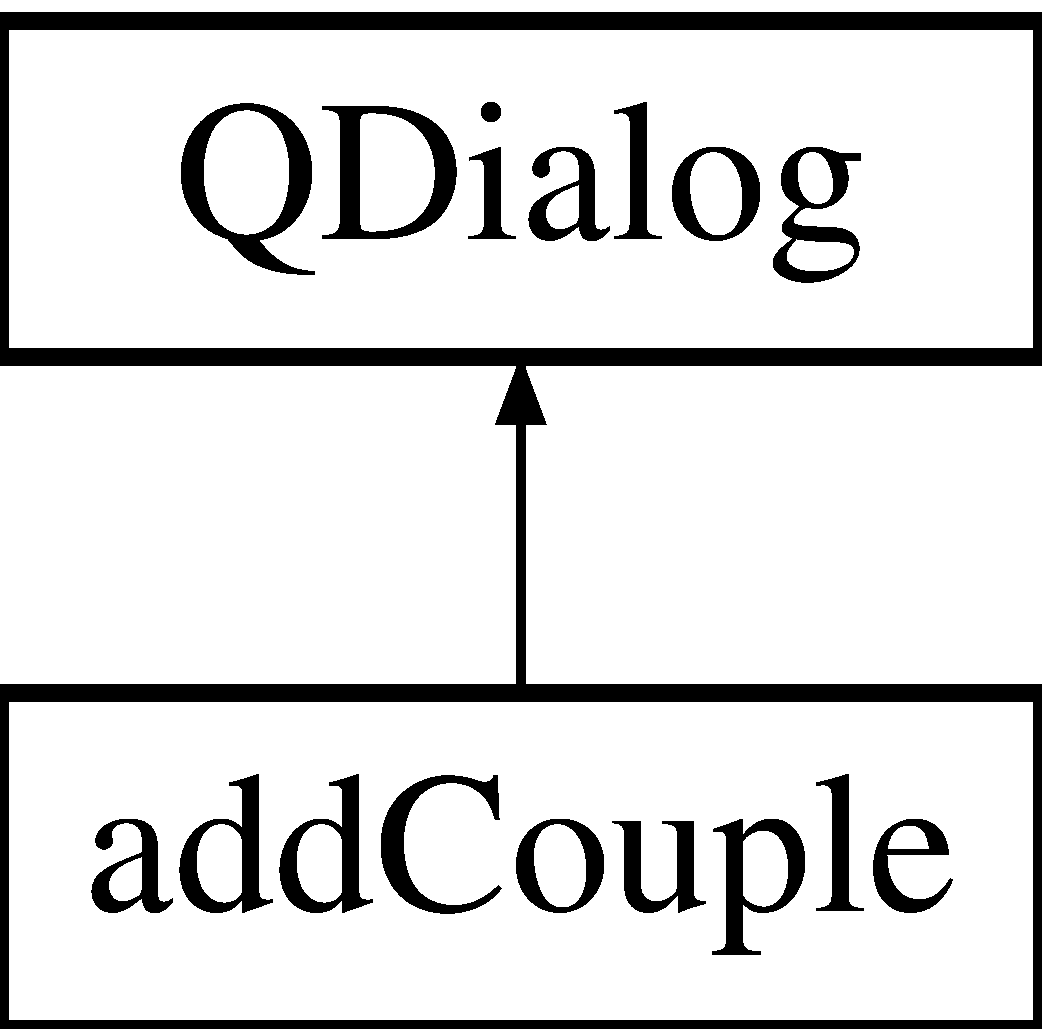
\includegraphics[height=2.000000cm]{classadd_couple}
\end{center}
\end{figure}
\subsection*{Public Slots}
\begin{DoxyCompactItemize}
\item 
\mbox{\Hypertarget{classadd_couple_aa0334cda3e89d32093da234cbd1e8c07}\label{classadd_couple_aa0334cda3e89d32093da234cbd1e8c07}} 
void {\bfseries update\+Model\+\_\+to} (Q\+Model\+Index index)
\item 
\mbox{\Hypertarget{classadd_couple_af8d724cab931e45a5e68a341fd831aca}\label{classadd_couple_af8d724cab931e45a5e68a341fd831aca}} 
void {\bfseries on\+\_\+to\+View\+\_\+clicked} (Q\+Model\+Index i)
\item 
\mbox{\Hypertarget{classadd_couple_ad3a6409a37b17097325d0b65ee1ab15b}\label{classadd_couple_ad3a6409a37b17097325d0b65ee1ab15b}} 
void {\bfseries on\+\_\+save\+\_\+clicked} ()
\end{DoxyCompactItemize}
\subsection*{Signals}
\begin{DoxyCompactItemize}
\item 
\mbox{\Hypertarget{classadd_couple_a2c807c5516dfa2ff6ecd00622914eb4c}\label{classadd_couple_a2c807c5516dfa2ff6ecd00622914eb4c}} 
void {\bfseries add\+New\+Couple} (Q\+String, Q\+String, Q\+String, bool)
\end{DoxyCompactItemize}
\subsection*{Public Member Functions}
\begin{DoxyCompactItemize}
\item 
\mbox{\Hypertarget{classadd_couple_a5c478c6e07cd0b9639c4c84687c89764}\label{classadd_couple_a5c478c6e07cd0b9639c4c84687c89764}} 
{\bfseries add\+Couple} (Q\+Widget $\ast$parent=0)
\end{DoxyCompactItemize}


\subsection{Detailed Description}


Definition at line 10 of file addcouple.\+h.



The documentation for this class was generated from the following files\+:\begin{DoxyCompactItemize}
\item 
addcouple.\+h\item 
addcouple.\+cpp\end{DoxyCompactItemize}

\hypertarget{class_append_text}{}\section{Append\+Text Class Reference}
\label{class_append_text}\index{Append\+Text@{Append\+Text}}
Inheritance diagram for Append\+Text\+:\begin{figure}[H]
\begin{center}
\leavevmode
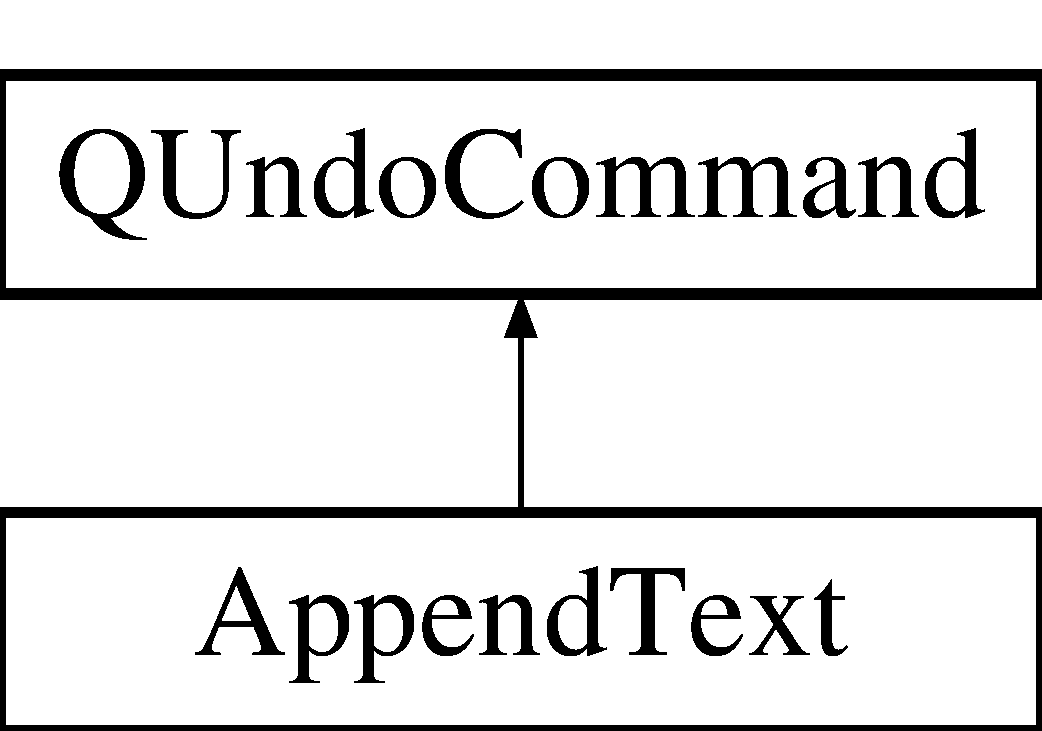
\includegraphics[height=2.000000cm]{class_append_text}
\end{center}
\end{figure}
\subsection*{Public Member Functions}
\begin{DoxyCompactItemize}
\item 
\mbox{\Hypertarget{class_append_text_a1f053473808df00e83d26566b5be19cd}\label{class_append_text_a1f053473808df00e83d26566b5be19cd}} 
{\bfseries Append\+Text} (Q\+String $\ast$doc, const Q\+String \&text)
\item 
\mbox{\Hypertarget{class_append_text_a9289ddb9645f35cc98e05e77d96ca093}\label{class_append_text_a9289ddb9645f35cc98e05e77d96ca093}} 
virtual void {\bfseries undo} ()
\item 
\mbox{\Hypertarget{class_append_text_a552142d5909b416eadbb4f6f728cb9d6}\label{class_append_text_a552142d5909b416eadbb4f6f728cb9d6}} 
virtual void {\bfseries redo} ()
\end{DoxyCompactItemize}


\subsection{Detailed Description}


Definition at line 19 of file undoredo.\+h.



The documentation for this class was generated from the following file\+:\begin{DoxyCompactItemize}
\item 
\hyperlink{undoredo_8h}{undoredo.\+h}\end{DoxyCompactItemize}

\hypertarget{class_article}{}\section{Article Class Reference}
\label{class_article}\index{Article@{Article}}


Inheritance diagram for Article\+:\nopagebreak
\begin{figure}[H]
\begin{center}
\leavevmode
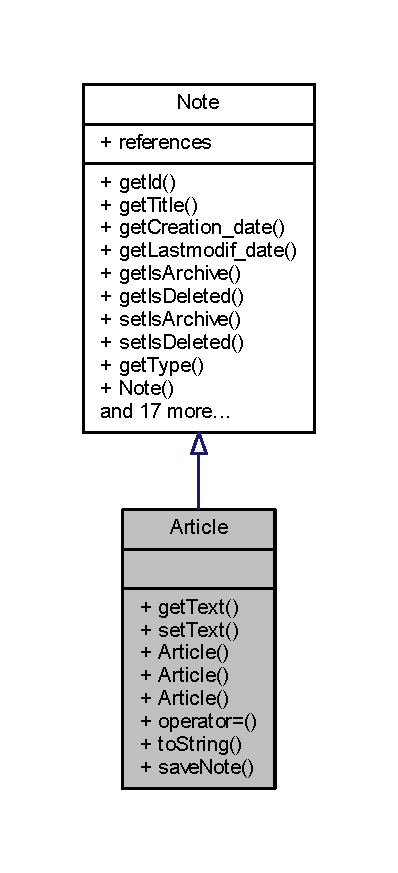
\includegraphics[width=191pt]{class_article__inherit__graph}
\end{center}
\end{figure}


Collaboration diagram for Article\+:\nopagebreak
\begin{figure}[H]
\begin{center}
\leavevmode
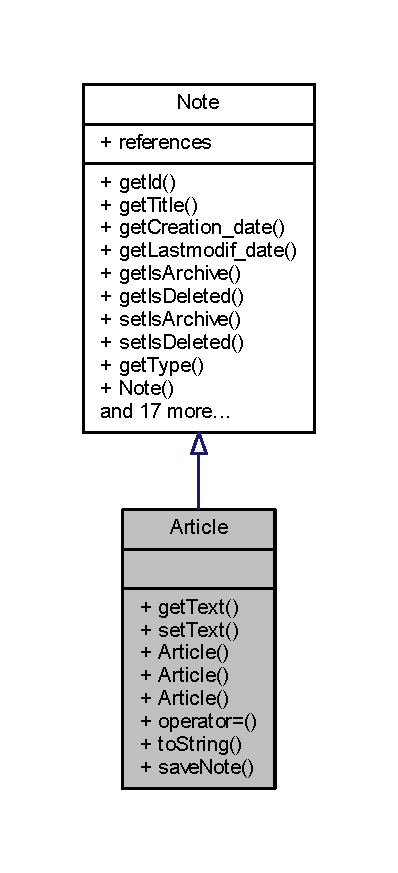
\includegraphics[width=191pt]{class_article__coll__graph}
\end{center}
\end{figure}
\subsection*{Public Member Functions}
\begin{DoxyCompactItemize}
\item 
const Q\+Text\+Document \& \hyperlink{class_article_a178a250fddb6c30288d893f4f3439ca8}{get\+Text} () const
\begin{DoxyCompactList}\small\item\em Accesseur du champ Text. \end{DoxyCompactList}\item 
void \hyperlink{class_article_a7144942027b1761cfcbd21761dd5cee8}{set\+Text} (const Q\+String \&t)
\begin{DoxyCompactList}\small\item\em Affectation du champ Text. \end{DoxyCompactList}\item 
\hyperlink{class_article_af3f6b98ba3cc46aaa5625a17266eb67f}{Article} (const Q\+String \&i, const Q\+String \&ti, const Q\+String \&te)
\begin{DoxyCompactList}\small\item\em Constructeur de la classe \hyperlink{class_article}{Article}. \end{DoxyCompactList}\item 
\mbox{\Hypertarget{class_article_a067e635213e9ff6b93fd8f88e471652f}\label{class_article_a067e635213e9ff6b93fd8f88e471652f}} 
{\bfseries Article} (const Q\+String \&i, const Q\+String \&ti, const Q\+Date\+Time \&cd, const Q\+Date\+Time \&lmd, bool iA, bool iD, const Q\+String \&te)
\item 
\mbox{\Hypertarget{class_article_a77eaa1a87e24eec7788f438a30ff162f}\label{class_article_a77eaa1a87e24eec7788f438a30ff162f}} 
\hyperlink{class_article_a77eaa1a87e24eec7788f438a30ff162f}{Article} (const \hyperlink{class_article}{Article} \&a)
\begin{DoxyCompactList}\small\item\em Surcharge la méthode constructeur dans le cas nouvel article \hyperlink{class_article}{Article} B(\+A) \end{DoxyCompactList}\item 
\hyperlink{class_article}{Article} \& \hyperlink{class_article_ae4059abc035598ff3faf554fd74a1492}{operator=} (const \hyperlink{class_article}{Article} \&a)
\begin{DoxyCompactList}\small\item\em Surcharge de l\textquotesingle{}opérateur = dans le cas nouvel article \hyperlink{class_article}{Article} B=A. \end{DoxyCompactList}\item 
std\+::string \hyperlink{class_article_ae40d268ecffbaaa549968a81ea609ba4}{to\+String} () const
\begin{DoxyCompactList}\small\item\em Transforme un article en un flux ostream a afficher. \end{DoxyCompactList}\item 
void \hyperlink{class_article_a83c6688e4886b871938b9dca34e78041}{save\+Note} (Q\+File $\ast$file)
\begin{DoxyCompactList}\small\item\em Fonction virtuelle permettant une sauvegarde personnalisée suivant le réel type de la note. \end{DoxyCompactList}\end{DoxyCompactItemize}
\subsection*{Additional Inherited Members}


\subsection{Detailed Description}


Definition at line 225 of file notes.\+h.



\subsection{Constructor \& Destructor Documentation}
\mbox{\Hypertarget{class_article_af3f6b98ba3cc46aaa5625a17266eb67f}\label{class_article_af3f6b98ba3cc46aaa5625a17266eb67f}} 
\index{Article@{Article}!Article@{Article}}
\index{Article@{Article}!Article@{Article}}
\subsubsection{\texorpdfstring{Article()}{Article()}}
{\footnotesize\ttfamily Article\+::\+Article (\begin{DoxyParamCaption}\item[{const Q\+String \&}]{i,  }\item[{const Q\+String \&}]{ti,  }\item[{const Q\+String \&}]{te }\end{DoxyParamCaption})}



Constructeur de la classe \hyperlink{class_article}{Article}. 

La classe dérivé \hyperlink{class_article}{Article} utilise en premier lieu le constructeur de \hyperlink{class_note}{Note}. 

Definition at line 135 of file notes.\+cpp.

Here is the call graph for this function\+:\nopagebreak
\begin{figure}[H]
\begin{center}
\leavevmode
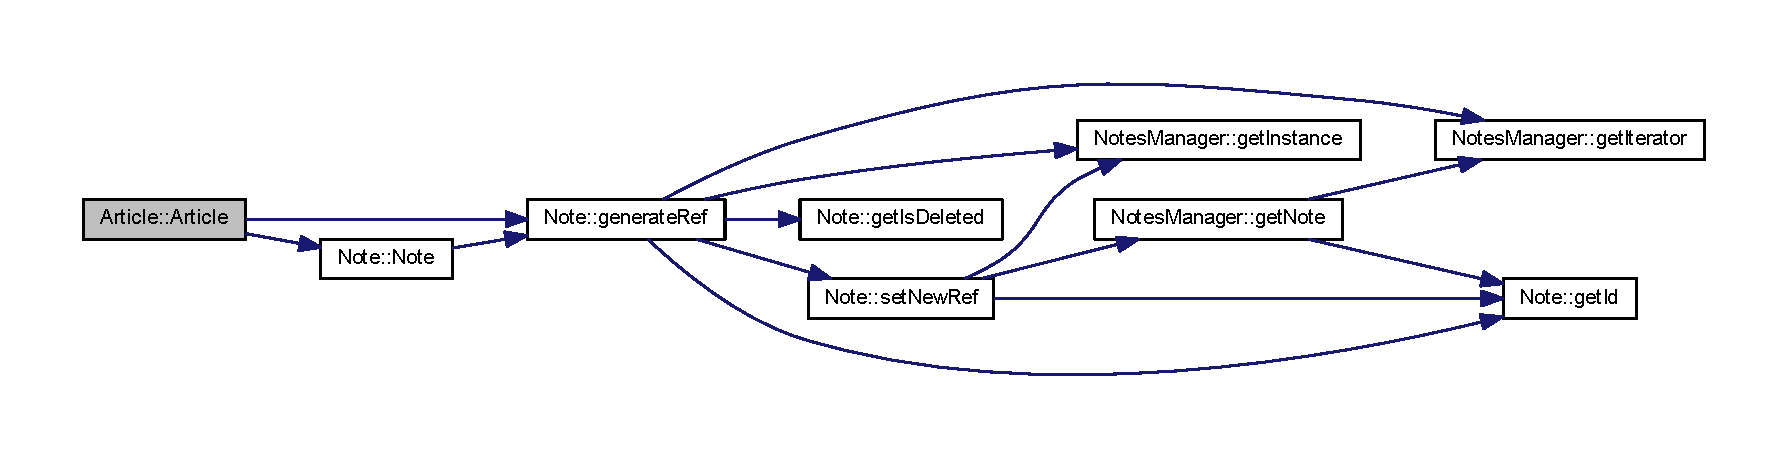
\includegraphics[width=350pt]{class_article_af3f6b98ba3cc46aaa5625a17266eb67f_cgraph}
\end{center}
\end{figure}


\subsection{Member Function Documentation}
\mbox{\Hypertarget{class_article_a178a250fddb6c30288d893f4f3439ca8}\label{class_article_a178a250fddb6c30288d893f4f3439ca8}} 
\index{Article@{Article}!get\+Text@{get\+Text}}
\index{get\+Text@{get\+Text}!Article@{Article}}
\subsubsection{\texorpdfstring{get\+Text()}{getText()}}
{\footnotesize\ttfamily const Q\+Text\+Document \& Article\+::get\+Text (\begin{DoxyParamCaption}{ }\end{DoxyParamCaption}) const\hspace{0.3cm}{\ttfamily [inline]}}



Accesseur du champ Text. 

\begin{DoxyReturn}{Returns}
const Q\+Text\+Document\& 
\end{DoxyReturn}


Definition at line 234 of file notes.\+h.

Here is the caller graph for this function\+:\nopagebreak
\begin{figure}[H]
\begin{center}
\leavevmode
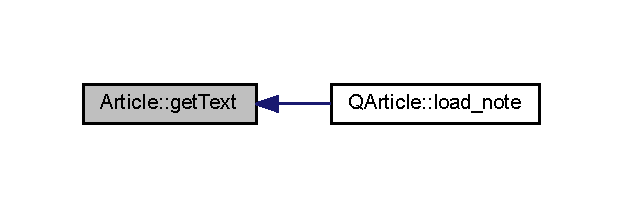
\includegraphics[width=299pt]{class_article_a178a250fddb6c30288d893f4f3439ca8_icgraph}
\end{center}
\end{figure}
\mbox{\Hypertarget{class_article_ae4059abc035598ff3faf554fd74a1492}\label{class_article_ae4059abc035598ff3faf554fd74a1492}} 
\index{Article@{Article}!operator=@{operator=}}
\index{operator=@{operator=}!Article@{Article}}
\subsubsection{\texorpdfstring{operator=()}{operator=()}}
{\footnotesize\ttfamily \hyperlink{class_article}{Article} \& Article\+::operator= (\begin{DoxyParamCaption}\item[{const \hyperlink{class_article}{Article} \&}]{a }\end{DoxyParamCaption})}



Surcharge de l\textquotesingle{}opérateur = dans le cas nouvel article \hyperlink{class_article}{Article} B=A. 

\begin{DoxyReturn}{Returns}
\hyperlink{class_article}{Article}\& 
\end{DoxyReturn}


Definition at line 53 of file notes.\+cpp.

Here is the call graph for this function\+:\nopagebreak
\begin{figure}[H]
\begin{center}
\leavevmode
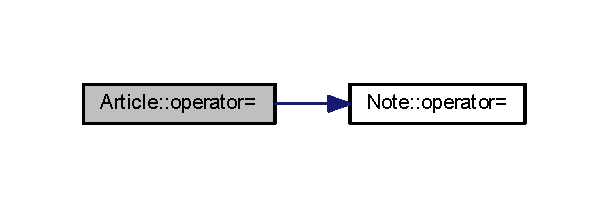
\includegraphics[width=292pt]{class_article_ae4059abc035598ff3faf554fd74a1492_cgraph}
\end{center}
\end{figure}
\mbox{\Hypertarget{class_article_a83c6688e4886b871938b9dca34e78041}\label{class_article_a83c6688e4886b871938b9dca34e78041}} 
\index{Article@{Article}!save\+Note@{save\+Note}}
\index{save\+Note@{save\+Note}!Article@{Article}}
\subsubsection{\texorpdfstring{save\+Note()}{saveNote()}}
{\footnotesize\ttfamily void Article\+::save\+Note (\begin{DoxyParamCaption}\item[{Q\+File $\ast$}]{file }\end{DoxyParamCaption})\hspace{0.3cm}{\ttfamily [virtual]}}



Fonction virtuelle permettant une sauvegarde personnalisée suivant le réel type de la note. 


\begin{DoxyParams}{Parameters}
{\em Q\+File$\ast$} & file \\
\hline
\end{DoxyParams}


Reimplemented from \hyperlink{class_note_a0c2cc72d7f3235c665a30ef915c5c58d}{Note}.



Definition at line 476 of file notes.\+cpp.

Here is the call graph for this function\+:\nopagebreak
\begin{figure}[H]
\begin{center}
\leavevmode
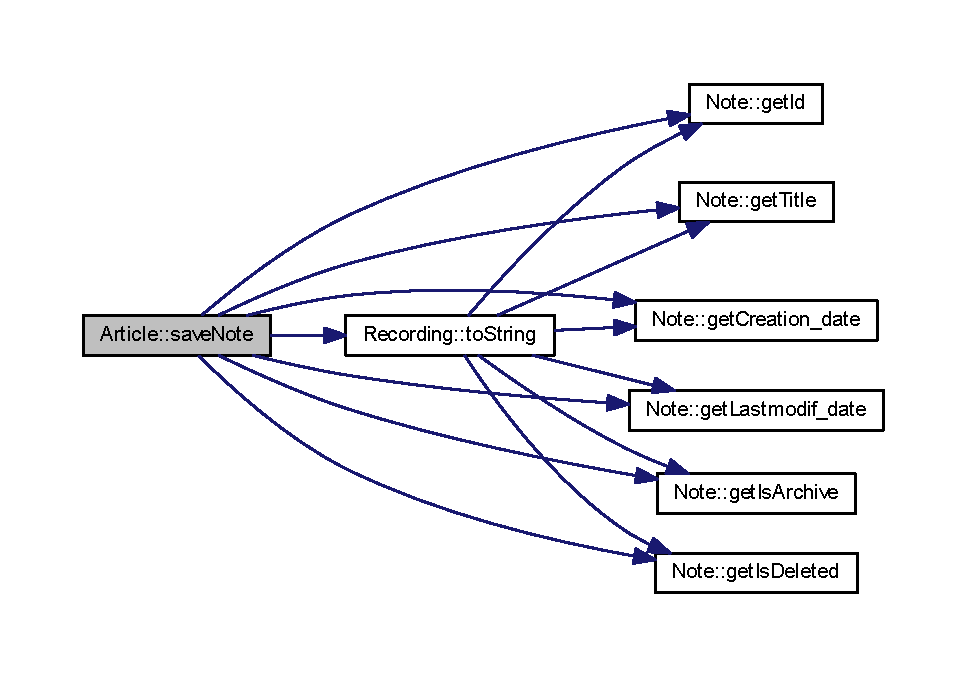
\includegraphics[width=350pt]{class_article_a83c6688e4886b871938b9dca34e78041_cgraph}
\end{center}
\end{figure}
\mbox{\Hypertarget{class_article_a7144942027b1761cfcbd21761dd5cee8}\label{class_article_a7144942027b1761cfcbd21761dd5cee8}} 
\index{Article@{Article}!set\+Text@{set\+Text}}
\index{set\+Text@{set\+Text}!Article@{Article}}
\subsubsection{\texorpdfstring{set\+Text()}{setText()}}
{\footnotesize\ttfamily void Article\+::set\+Text (\begin{DoxyParamCaption}\item[{const Q\+String \&}]{t }\end{DoxyParamCaption})\hspace{0.3cm}{\ttfamily [inline]}}



Affectation du champ Text. 


\begin{DoxyParams}{Parameters}
{\em const} & Q\+String\& \\
\hline
\end{DoxyParams}


Definition at line 240 of file notes.\+h.

Here is the caller graph for this function\+:\nopagebreak
\begin{figure}[H]
\begin{center}
\leavevmode
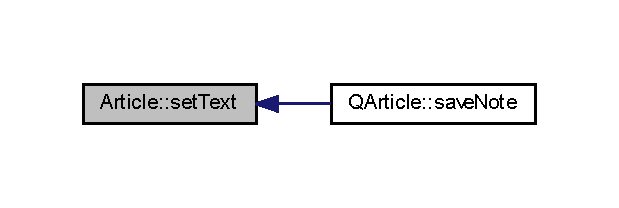
\includegraphics[width=297pt]{class_article_a7144942027b1761cfcbd21761dd5cee8_icgraph}
\end{center}
\end{figure}
\mbox{\Hypertarget{class_article_ae40d268ecffbaaa549968a81ea609ba4}\label{class_article_ae40d268ecffbaaa549968a81ea609ba4}} 
\index{Article@{Article}!to\+String@{to\+String}}
\index{to\+String@{to\+String}!Article@{Article}}
\subsubsection{\texorpdfstring{to\+String()}{toString()}}
{\footnotesize\ttfamily std\+::string Article\+::to\+String (\begin{DoxyParamCaption}{ }\end{DoxyParamCaption}) const\hspace{0.3cm}{\ttfamily [virtual]}}



Transforme un article en un flux ostream a afficher. 

\begin{DoxyReturn}{Returns}
Le flux ostream 
\end{DoxyReturn}


Reimplemented from \hyperlink{class_note_a1bd4acfbde0b71d05fd7d4ca889bca2b}{Note}.



Definition at line 199 of file notes.\+cpp.

Here is the call graph for this function\+:\nopagebreak
\begin{figure}[H]
\begin{center}
\leavevmode
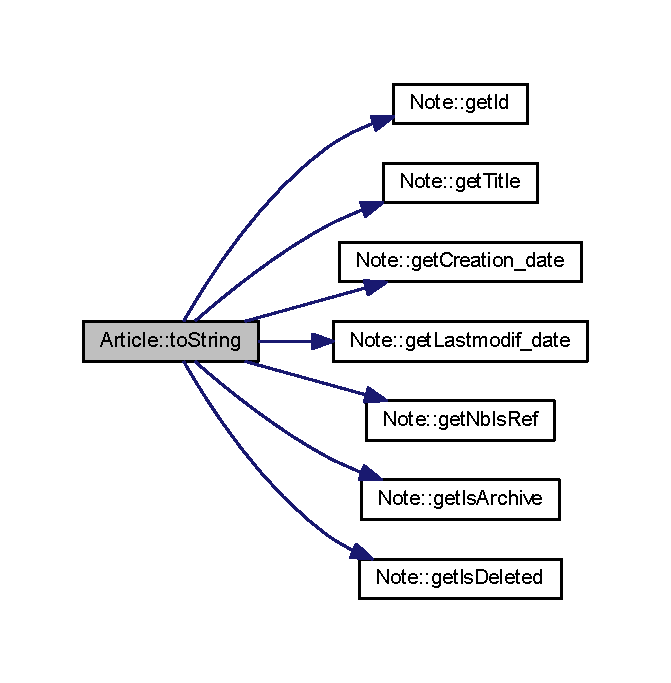
\includegraphics[width=322pt]{class_article_ae40d268ecffbaaa549968a81ea609ba4_cgraph}
\end{center}
\end{figure}


The documentation for this class was generated from the following files\+:\begin{DoxyCompactItemize}
\item 
O\+L13/\hyperlink{notes_8h}{notes.\+h}\item 
O\+L13/\hyperlink{notes_8cpp}{notes.\+cpp}\end{DoxyCompactItemize}

\hypertarget{class_creation___note}{}\section{Creation\+\_\+\+Note Class Reference}
\label{class_creation___note}\index{Creation\+\_\+\+Note@{Creation\+\_\+\+Note}}


Inheritance diagram for Creation\+\_\+\+Note\+:
\nopagebreak
\begin{figure}[H]
\begin{center}
\leavevmode
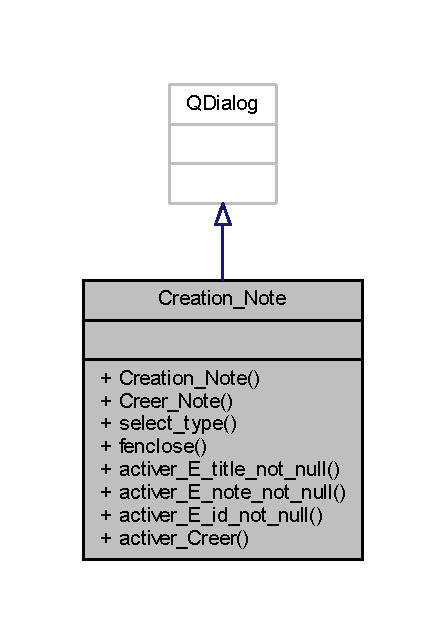
\includegraphics[width=214pt]{class_creation___note__inherit__graph}
\end{center}
\end{figure}


Collaboration diagram for Creation\+\_\+\+Note\+:
\nopagebreak
\begin{figure}[H]
\begin{center}
\leavevmode
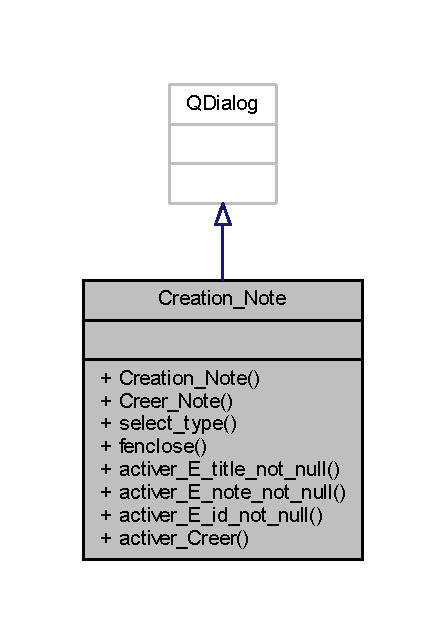
\includegraphics[width=214pt]{class_creation___note__coll__graph}
\end{center}
\end{figure}
\subsection*{Public Slots}
\begin{DoxyCompactItemize}
\item 
\mbox{\Hypertarget{class_creation___note_a533d14d9799dfb6257de99778d38a8ba}\label{class_creation___note_a533d14d9799dfb6257de99778d38a8ba}} 
void {\bfseries Creer\+\_\+\+Note} ()
\item 
\mbox{\Hypertarget{class_creation___note_a4627e5957db87af2b7c43937857e9d6e}\label{class_creation___note_a4627e5957db87af2b7c43937857e9d6e}} 
void {\bfseries select\+\_\+type} (int type)
\item 
\mbox{\Hypertarget{class_creation___note_a280ec768b1c2b99bdf885089c32c0134}\label{class_creation___note_a280ec768b1c2b99bdf885089c32c0134}} 
void {\bfseries fenclose} ()
\item 
\mbox{\Hypertarget{class_creation___note_a2b9c2eabbcff615f1f02f092a4706295}\label{class_creation___note_a2b9c2eabbcff615f1f02f092a4706295}} 
void {\bfseries activer\+\_\+\+E\+\_\+title\+\_\+not\+\_\+null} ()
\item 
\mbox{\Hypertarget{class_creation___note_a55a85cdf537406058368bbdb3d3e8ed1}\label{class_creation___note_a55a85cdf537406058368bbdb3d3e8ed1}} 
void {\bfseries activer\+\_\+\+E\+\_\+note\+\_\+not\+\_\+null} (bool status)
\item 
\mbox{\Hypertarget{class_creation___note_abe23b774f4d9964f6d745d4c1d6e1621}\label{class_creation___note_abe23b774f4d9964f6d745d4c1d6e1621}} 
void {\bfseries activer\+\_\+\+E\+\_\+id\+\_\+not\+\_\+null} ()
\item 
\mbox{\Hypertarget{class_creation___note_a07b8f673a499c2cf3b47ff990b7c80ef}\label{class_creation___note_a07b8f673a499c2cf3b47ff990b7c80ef}} 
void {\bfseries activer\+\_\+\+Creer} ()
\end{DoxyCompactItemize}
\subsection*{Signals}
\begin{DoxyCompactItemize}
\item 
\mbox{\Hypertarget{class_creation___note_ac077793d8161d266c9d500c6545da80e}\label{class_creation___note_ac077793d8161d266c9d500c6545da80e}} 
void {\bfseries change\+\_\+\+Creer} ()
\item 
\mbox{\Hypertarget{class_creation___note_a51d4541fbf18ccb297ce5f15da3a6cab}\label{class_creation___note_a51d4541fbf18ccb297ce5f15da3a6cab}} 
void {\bfseries new\+Note} (\hyperlink{class_note}{Note} \&n)
\end{DoxyCompactItemize}
\subsection*{Public Member Functions}
\begin{DoxyCompactItemize}
\item 
\mbox{\Hypertarget{class_creation___note_a76278cf9f0de87cd61f204aafcebd5d2}\label{class_creation___note_a76278cf9f0de87cd61f204aafcebd5d2}} 
{\bfseries Creation\+\_\+\+Note} (Q\+Widget $\ast$parent)
\end{DoxyCompactItemize}


\subsection{Detailed Description}


Definition at line 19 of file Creation\+\_\+\+Note.\+h.



The documentation for this class was generated from the following files\+:\begin{DoxyCompactItemize}
\item 
O\+L13/\hyperlink{_creation___note_8h}{Creation\+\_\+\+Note.\+h}\item 
O\+L13/\hyperlink{_creation___note_8cpp}{Creation\+\_\+\+Note.\+cpp}\end{DoxyCompactItemize}

\hypertarget{class_deleted_note}{}\section{Deleted\+Note Class Reference}
\label{class_deleted_note}\index{Deleted\+Note@{Deleted\+Note}}


Inheritance diagram for Deleted\+Note\+:\nopagebreak
\begin{figure}[H]
\begin{center}
\leavevmode
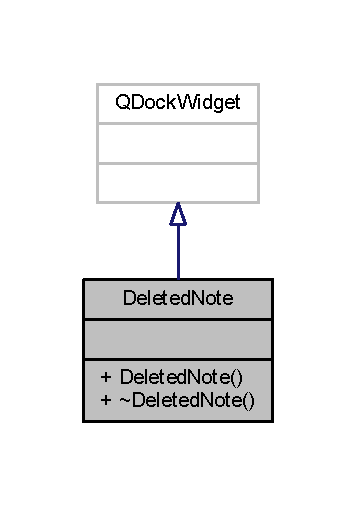
\includegraphics[width=171pt]{class_deleted_note__inherit__graph}
\end{center}
\end{figure}


Collaboration diagram for Deleted\+Note\+:\nopagebreak
\begin{figure}[H]
\begin{center}
\leavevmode
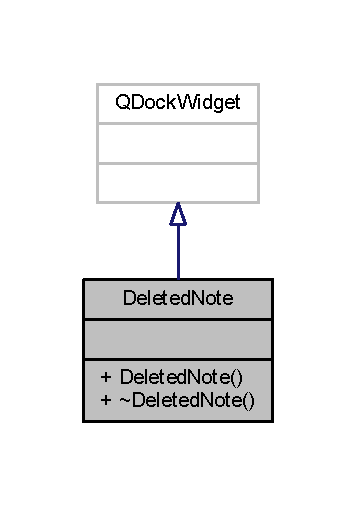
\includegraphics[width=171pt]{class_deleted_note__coll__graph}
\end{center}
\end{figure}
\subsection*{Public Member Functions}
\begin{DoxyCompactItemize}
\item 
\mbox{\Hypertarget{class_deleted_note_a23fe178b1e3f593b9ac1957e44271e7e}\label{class_deleted_note_a23fe178b1e3f593b9ac1957e44271e7e}} 
{\bfseries Deleted\+Note} (Q\+Widget $\ast$parent=0)
\end{DoxyCompactItemize}


\subsection{Detailed Description}


Definition at line 10 of file deletednote.\+h.



The documentation for this class was generated from the following files\+:\begin{DoxyCompactItemize}
\item 
O\+L13/deletednote.\+h\item 
O\+L13/deletednote.\+cpp\end{DoxyCompactItemize}

\hypertarget{class_dock}{}\section{Dock Class Reference}
\label{class_dock}\index{Dock@{Dock}}
Inheritance diagram for Dock\+:\begin{figure}[H]
\begin{center}
\leavevmode
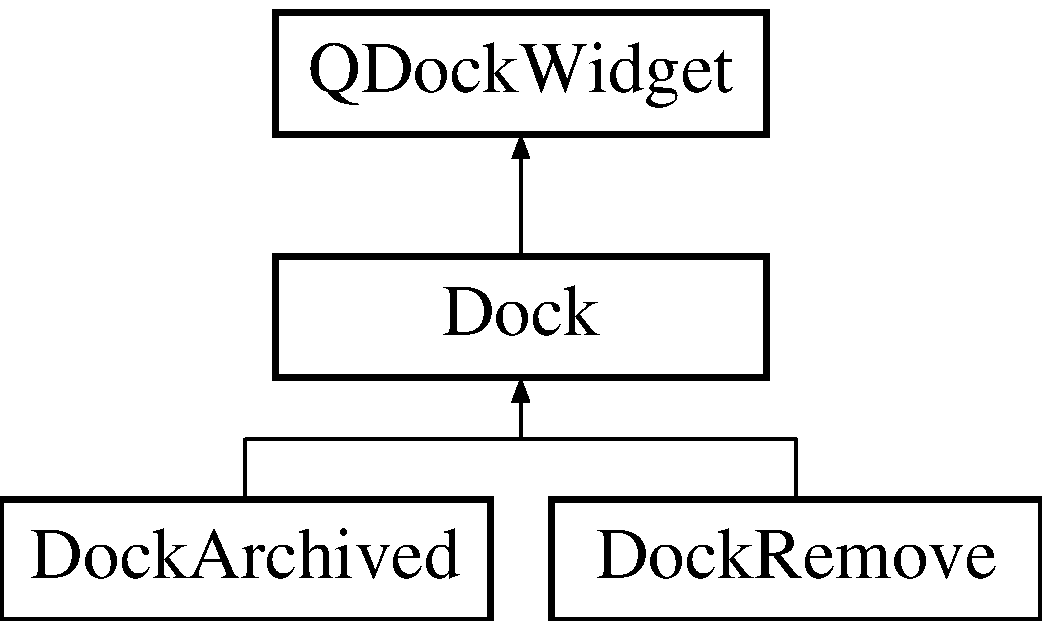
\includegraphics[height=3.000000cm]{class_dock}
\end{center}
\end{figure}
\subsection*{Public Slots}
\begin{DoxyCompactItemize}
\item 
\mbox{\Hypertarget{class_dock_a74bd1a9145a04fe37c1c97bedd7c460d}\label{class_dock_a74bd1a9145a04fe37c1c97bedd7c460d}} 
virtual void {\bfseries on\+\_\+remove\+\_\+clicked} ()=0
\item 
\mbox{\Hypertarget{class_dock_aba7e136be0e7bbff8cf76369e10982c0}\label{class_dock_aba7e136be0e7bbff8cf76369e10982c0}} 
virtual void {\bfseries update\+\_\+arch\+Note\+Model} ()=0
\item 
\mbox{\Hypertarget{class_dock_a162f55159baba3ad2f485c1cbfb67fe2}\label{class_dock_a162f55159baba3ad2f485c1cbfb67fe2}} 
void {\bfseries on\+\_\+aff\+\_\+clicked} ()
\item 
\mbox{\Hypertarget{class_dock_a88d9948db78eddd5551bb47e4cb63277}\label{class_dock_a88d9948db78eddd5551bb47e4cb63277}} 
void {\bfseries on\+\_\+\+Arch\+View\+\_\+clicked} (Q\+Model\+Index i)
\end{DoxyCompactItemize}
\subsection*{Signals}
\begin{DoxyCompactItemize}
\item 
\mbox{\Hypertarget{class_dock_aca603632e4561e582254273c234d97a8}\label{class_dock_aca603632e4561e582254273c234d97a8}} 
void {\bfseries update\+\_\+remove\+Dock} ()
\item 
\mbox{\Hypertarget{class_dock_a8abd37c4496e6c548ecb4ecb685679a1}\label{class_dock_a8abd37c4496e6c548ecb4ecb685679a1}} 
void {\bfseries selection} (Q\+String, int)
\end{DoxyCompactItemize}
\subsection*{Public Member Functions}
\begin{DoxyCompactItemize}
\item 
\mbox{\Hypertarget{class_dock_a1e81e2926e94969514ac45a9d839731c}\label{class_dock_a1e81e2926e94969514ac45a9d839731c}} 
{\bfseries Dock} (Q\+Widget $\ast$parent=0)
\end{DoxyCompactItemize}
\subsection*{Protected Attributes}
\begin{DoxyCompactItemize}
\item 
\mbox{\Hypertarget{class_dock_a525f557d9a2670640105da2f1e605026}\label{class_dock_a525f557d9a2670640105da2f1e605026}} 
Ui\+::\+Dock\+Archived $\ast$ {\bfseries ui}
\item 
\mbox{\Hypertarget{class_dock_a6af86621e3df52266a582e464324e6d2}\label{class_dock_a6af86621e3df52266a582e464324e6d2}} 
Q\+String {\bfseries current\+Note}
\item 
\mbox{\Hypertarget{class_dock_a484517393b214e1c3abe0c7b36596172}\label{class_dock_a484517393b214e1c3abe0c7b36596172}} 
Q\+Standard\+Item\+Model $\ast$ {\bfseries Arch\+Note}
\end{DoxyCompactItemize}


\subsection{Detailed Description}


Definition at line 11 of file dockarchived.\+h.



The documentation for this class was generated from the following files\+:\begin{DoxyCompactItemize}
\item 
O\+L13/dockarchived.\+h\item 
O\+L13/dockarchived.\+cpp\end{DoxyCompactItemize}

\hypertarget{class_dock_archived}{}\section{Dock\+Archived Class Reference}
\label{class_dock_archived}\index{Dock\+Archived@{Dock\+Archived}}
Inheritance diagram for Dock\+Archived\+:\begin{figure}[H]
\begin{center}
\leavevmode
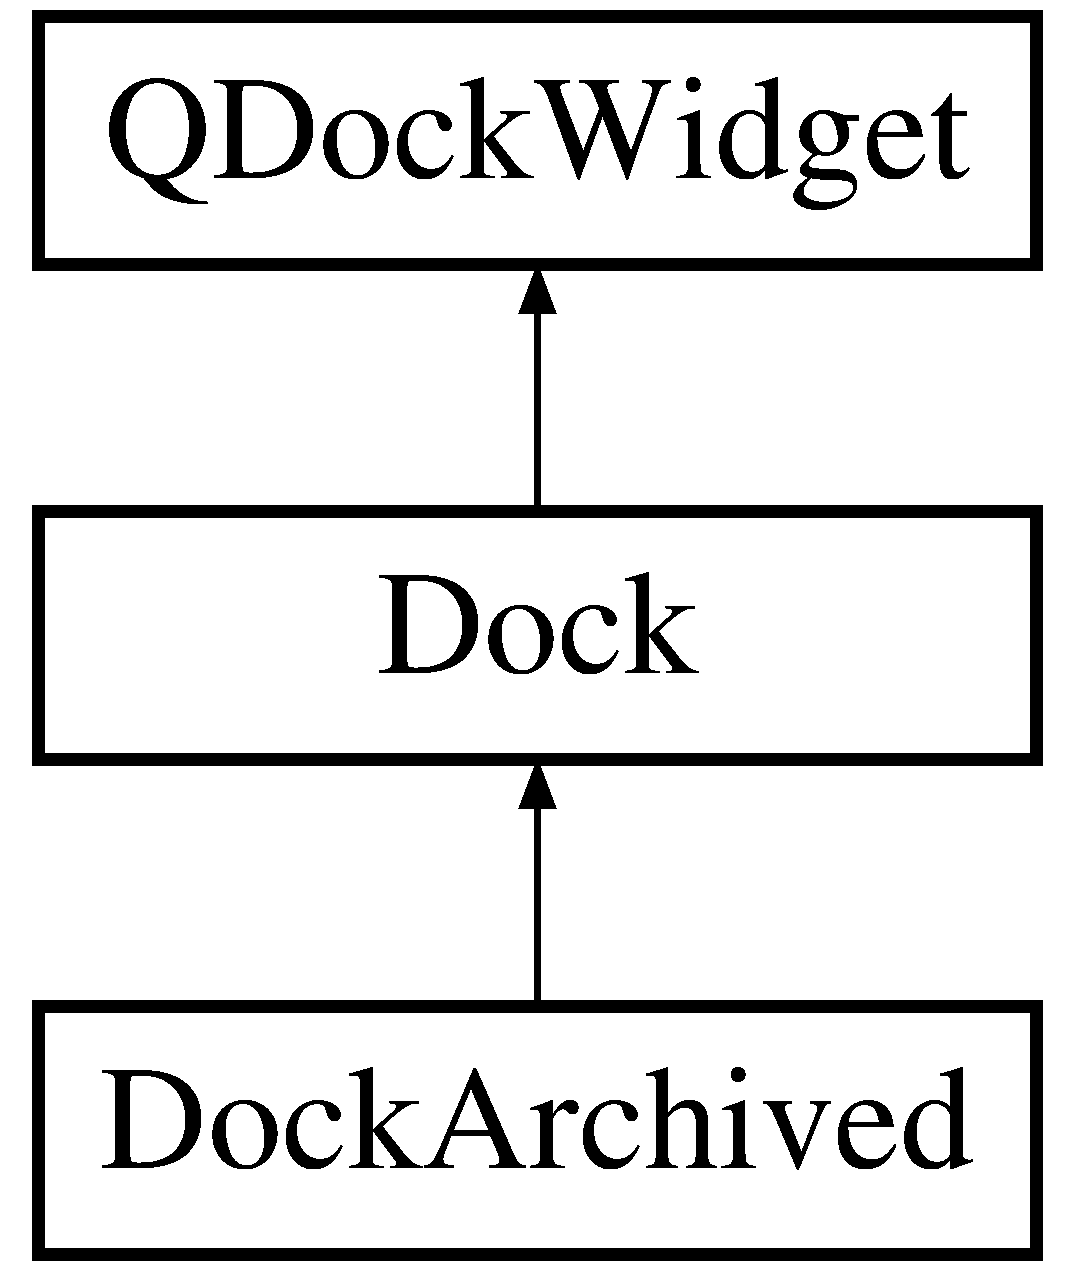
\includegraphics[height=3.000000cm]{class_dock_archived}
\end{center}
\end{figure}
\subsection*{Public Slots}
\begin{DoxyCompactItemize}
\item 
\mbox{\Hypertarget{class_dock_archived_ab2ec83022057fff8169784cf02876a8a}\label{class_dock_archived_ab2ec83022057fff8169784cf02876a8a}} 
void {\bfseries on\+\_\+remove\+\_\+clicked} ()
\end{DoxyCompactItemize}
\subsection*{Public Member Functions}
\begin{DoxyCompactItemize}
\item 
\mbox{\Hypertarget{class_dock_archived_ad3cc1b3cbaa84fed8d37c478927c7463}\label{class_dock_archived_ad3cc1b3cbaa84fed8d37c478927c7463}} 
{\bfseries Dock\+Archived} (Q\+Widget $\ast$parent)
\item 
\mbox{\Hypertarget{class_dock_archived_a557ea9fc3b685f0aefbae0bcd624cbec}\label{class_dock_archived_a557ea9fc3b685f0aefbae0bcd624cbec}} 
void {\bfseries update\+\_\+arch\+Note\+Model} ()
\end{DoxyCompactItemize}
\subsection*{Additional Inherited Members}


\subsection{Detailed Description}


Definition at line 34 of file dockarchived.\+h.



The documentation for this class was generated from the following files\+:\begin{DoxyCompactItemize}
\item 
dockarchived.\+h\item 
dockarchived.\+cpp\end{DoxyCompactItemize}

\hypertarget{class_dock_remove}{}\section{Dock\+Remove Class Reference}
\label{class_dock_remove}\index{Dock\+Remove@{Dock\+Remove}}


Inheritance diagram for Dock\+Remove\+:\nopagebreak
\begin{figure}[H]
\begin{center}
\leavevmode
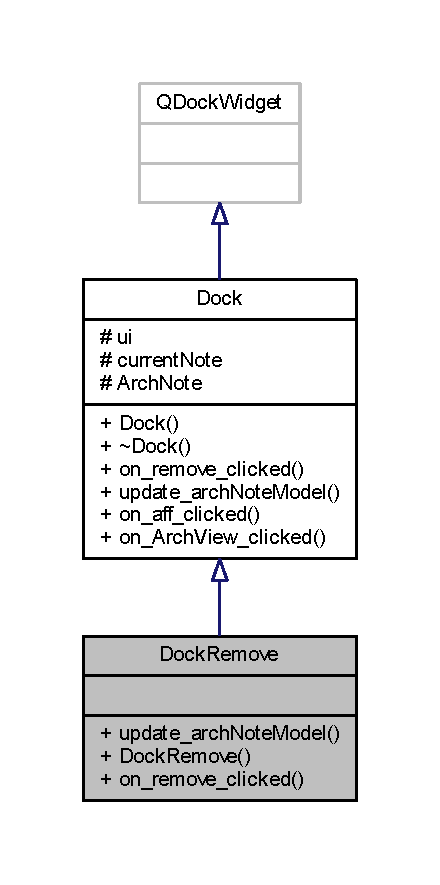
\includegraphics[width=211pt]{class_dock_remove__inherit__graph}
\end{center}
\end{figure}


Collaboration diagram for Dock\+Remove\+:\nopagebreak
\begin{figure}[H]
\begin{center}
\leavevmode
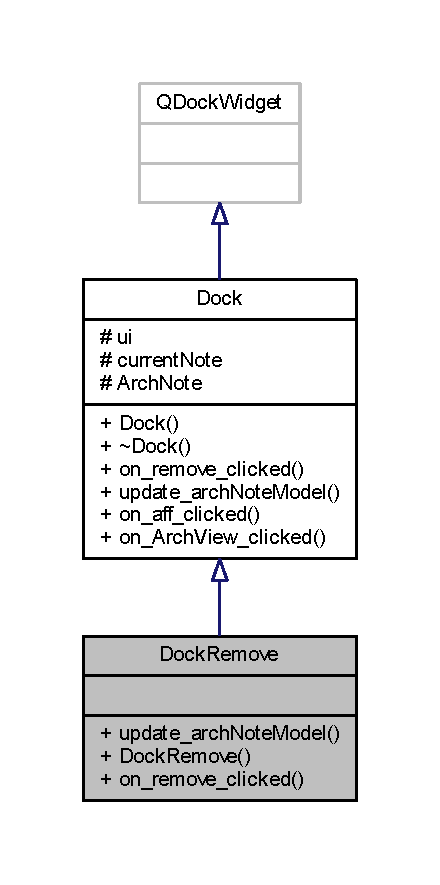
\includegraphics[width=211pt]{class_dock_remove__coll__graph}
\end{center}
\end{figure}
\subsection*{Public Slots}
\begin{DoxyCompactItemize}
\item 
\mbox{\Hypertarget{class_dock_remove_af674d9505592df25cd5b08328c0cdbd6}\label{class_dock_remove_af674d9505592df25cd5b08328c0cdbd6}} 
void {\bfseries on\+\_\+remove\+\_\+clicked} ()
\end{DoxyCompactItemize}
\subsection*{Public Member Functions}
\begin{DoxyCompactItemize}
\item 
\mbox{\Hypertarget{class_dock_remove_a4e653c9a21161b7d76c9cfd330579047}\label{class_dock_remove_a4e653c9a21161b7d76c9cfd330579047}} 
void \hyperlink{class_dock_remove_a4e653c9a21161b7d76c9cfd330579047}{update\+\_\+arch\+Note\+Model} ()
\begin{DoxyCompactList}\small\item\em Mise à jour du \hyperlink{class_dock}{Dock} des éléments supprimés. \end{DoxyCompactList}\item 
\hyperlink{class_dock_remove_aa2665bd1459600d9346029df9f2bba27}{Dock\+Remove} (Q\+Widget $\ast$parent)
\begin{DoxyCompactList}\small\item\em Constructeur du \hyperlink{class_dock}{Dock} des éléments supprimés. \end{DoxyCompactList}\end{DoxyCompactItemize}
\subsection*{Additional Inherited Members}


\subsection{Detailed Description}


Definition at line 84 of file dockarchived.\+h.



\subsection{Constructor \& Destructor Documentation}
\mbox{\Hypertarget{class_dock_remove_aa2665bd1459600d9346029df9f2bba27}\label{class_dock_remove_aa2665bd1459600d9346029df9f2bba27}} 
\index{Dock\+Remove@{Dock\+Remove}!Dock\+Remove@{Dock\+Remove}}
\index{Dock\+Remove@{Dock\+Remove}!Dock\+Remove@{Dock\+Remove}}
\subsubsection{\texorpdfstring{Dock\+Remove()}{DockRemove()}}
{\footnotesize\ttfamily Dock\+Remove\+::\+Dock\+Remove (\begin{DoxyParamCaption}\item[{Q\+Widget $\ast$}]{parent }\end{DoxyParamCaption})}



Constructeur du \hyperlink{class_dock}{Dock} des éléments supprimés. 


\begin{DoxyParams}{Parameters}
{\em parent} & \\
\hline
\end{DoxyParams}


Definition at line 96 of file dockarchived.\+cpp.



The documentation for this class was generated from the following files\+:\begin{DoxyCompactItemize}
\item 
O\+L13/\hyperlink{dockarchived_8h}{dockarchived.\+h}\item 
O\+L13/\hyperlink{dockarchived_8cpp}{dockarchived.\+cpp}\end{DoxyCompactItemize}

\hypertarget{class_edit___notes_couple}{}\section{Edit\+\_\+\+Notes\+Couple Class Reference}
\label{class_edit___notes_couple}\index{Edit\+\_\+\+Notes\+Couple@{Edit\+\_\+\+Notes\+Couple}}


Inheritance diagram for Edit\+\_\+\+Notes\+Couple\+:
\nopagebreak
\begin{figure}[H]
\begin{center}
\leavevmode
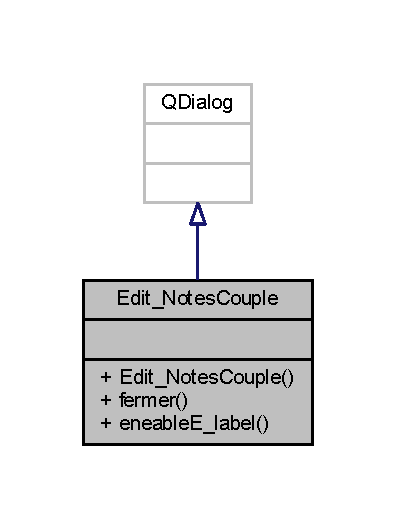
\includegraphics[width=190pt]{class_edit___notes_couple__inherit__graph}
\end{center}
\end{figure}


Collaboration diagram for Edit\+\_\+\+Notes\+Couple\+:
\nopagebreak
\begin{figure}[H]
\begin{center}
\leavevmode
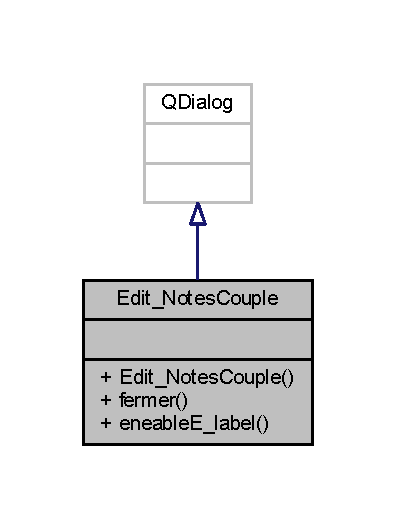
\includegraphics[width=190pt]{class_edit___notes_couple__coll__graph}
\end{center}
\end{figure}
\subsection*{Public Slots}
\begin{DoxyCompactItemize}
\item 
\mbox{\Hypertarget{class_edit___notes_couple_a4eb0c74a8e7428aa585136878ddf1edb}\label{class_edit___notes_couple_a4eb0c74a8e7428aa585136878ddf1edb}} 
void {\bfseries fermer} ()
\item 
\mbox{\Hypertarget{class_edit___notes_couple_ad51b47f9284bea44cddc186674c57bc9}\label{class_edit___notes_couple_ad51b47f9284bea44cddc186674c57bc9}} 
void {\bfseries eneable\+E\+\_\+label} ()
\end{DoxyCompactItemize}
\subsection*{Signals}
\begin{DoxyCompactItemize}
\item 
\mbox{\Hypertarget{class_edit___notes_couple_a4cf6489e93bef94d95fe460b195ba13d}\label{class_edit___notes_couple_a4cf6489e93bef94d95fe460b195ba13d}} 
void {\bfseries new\+Couple} (\hyperlink{class_note}{Note} $\ast$, \hyperlink{class_note}{Note} $\ast$, Q\+String, bool)
\item 
\mbox{\Hypertarget{class_edit___notes_couple_af5c4267cc253eb46628a89e2f14dadf6}\label{class_edit___notes_couple_af5c4267cc253eb46628a89e2f14dadf6}} 
void {\bfseries set\+Couple} (Q\+String)
\end{DoxyCompactItemize}
\subsection*{Public Member Functions}
\begin{DoxyCompactItemize}
\item 
\hyperlink{class_edit___notes_couple_aa0780f3a53175747c5a7136d4f2ffa30}{Edit\+\_\+\+Notes\+Couple} (\hyperlink{class_note}{Note} $\ast$n1, \hyperlink{class_note}{Note} $\ast$n2, Q\+Widget $\ast$parent=nullptr, bool s=false)
\end{DoxyCompactItemize}


\subsection{Detailed Description}


Definition at line 60 of file qrelations.\+h.



\subsection{Constructor \& Destructor Documentation}
\mbox{\Hypertarget{class_edit___notes_couple_aa0780f3a53175747c5a7136d4f2ffa30}\label{class_edit___notes_couple_aa0780f3a53175747c5a7136d4f2ffa30}} 
\index{Edit\+\_\+\+Notes\+Couple@{Edit\+\_\+\+Notes\+Couple}!Edit\+\_\+\+Notes\+Couple@{Edit\+\_\+\+Notes\+Couple}}
\index{Edit\+\_\+\+Notes\+Couple@{Edit\+\_\+\+Notes\+Couple}!Edit\+\_\+\+Notes\+Couple@{Edit\+\_\+\+Notes\+Couple}}
\subsubsection{\texorpdfstring{Edit\+\_\+\+Notes\+Couple()}{Edit\_NotesCouple()}}
{\footnotesize\ttfamily Edit\+\_\+\+Notes\+Couple\+::\+Edit\+\_\+\+Notes\+Couple (\begin{DoxyParamCaption}\item[{\hyperlink{class_note}{Note} $\ast$}]{n1,  }\item[{\hyperlink{class_note}{Note} $\ast$}]{n2,  }\item[{Q\+Widget $\ast$}]{parent = {\ttfamily nullptr},  }\item[{bool}]{s = {\ttfamily false} }\end{DoxyParamCaption})}

Connect\+: 

Definition at line 188 of file qrelations.\+cpp.



The documentation for this class was generated from the following files\+:\begin{DoxyCompactItemize}
\item 
O\+L13/qrelations.\+h\item 
O\+L13/qrelations.\+cpp\end{DoxyCompactItemize}

\hypertarget{class_edit__relation}{}\section{Edit\+\_\+relation Class Reference}
\label{class_edit__relation}\index{Edit\+\_\+relation@{Edit\+\_\+relation}}
Inheritance diagram for Edit\+\_\+relation\+:\begin{figure}[H]
\begin{center}
\leavevmode
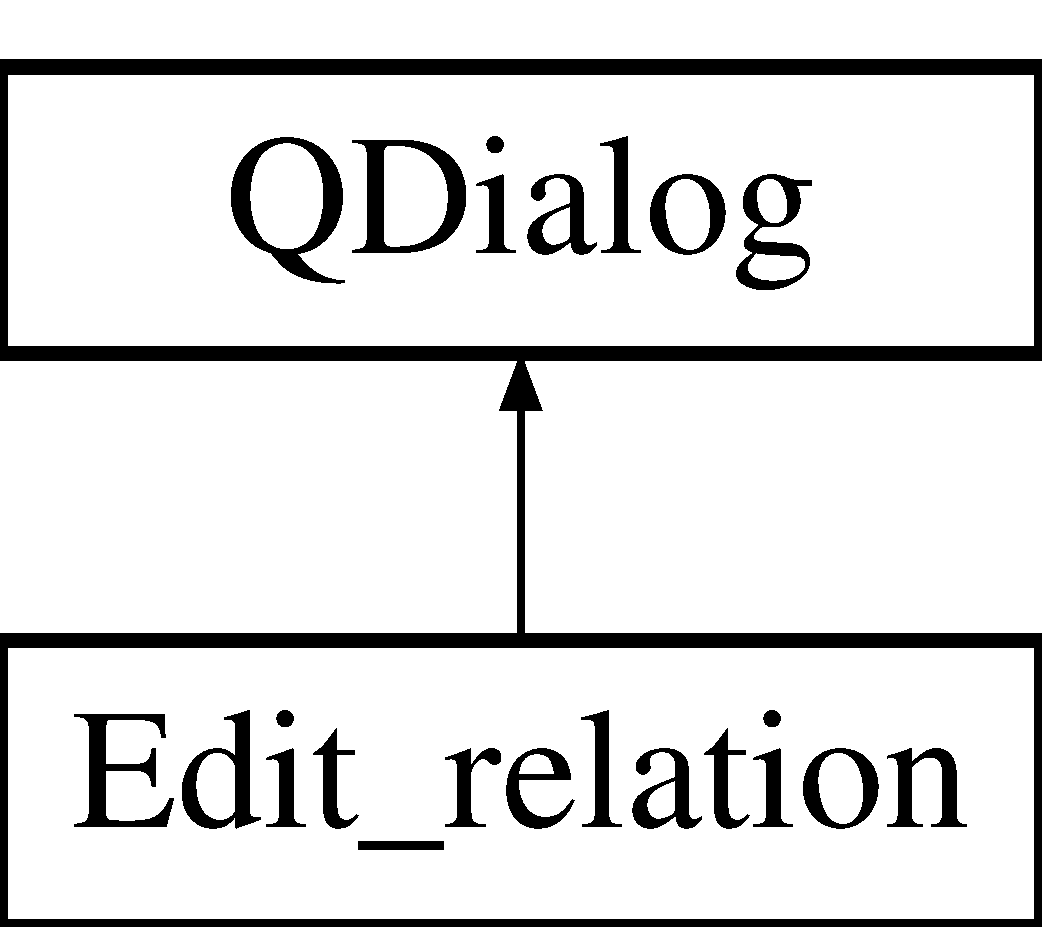
\includegraphics[height=2.000000cm]{class_edit__relation}
\end{center}
\end{figure}
\subsection*{Public Slots}
\begin{DoxyCompactItemize}
\item 
\mbox{\Hypertarget{class_edit__relation_ab8b401c68bf851bea39fc38fbce0f9f5}\label{class_edit__relation_ab8b401c68bf851bea39fc38fbce0f9f5}} 
void {\bfseries clic\+Selection} ()
\item 
\mbox{\Hypertarget{class_edit__relation_a558f8134fbd20281e24ceb350882ddaf}\label{class_edit__relation_a558f8134fbd20281e24ceb350882ddaf}} 
void {\bfseries enabled\+Append} ()
\item 
\mbox{\Hypertarget{class_edit__relation_a06254b8a5265ba82160c6ab62bbf9101}\label{class_edit__relation_a06254b8a5265ba82160c6ab62bbf9101}} 
void {\bfseries add\+Couple} (\hyperlink{class_note}{Note} $\ast$n1, \hyperlink{class_note}{Note} $\ast$n2, Q\+String label, bool s)
\end{DoxyCompactItemize}
\subsection*{Signals}
\begin{DoxyCompactItemize}
\item 
\mbox{\Hypertarget{class_edit__relation_a39ece696a8813495b806fcd5cc8ec51c}\label{class_edit__relation_a39ece696a8813495b806fcd5cc8ec51c}} 
void {\bfseries new\+Relation} ()
\end{DoxyCompactItemize}
\subsection*{Public Member Functions}
\begin{DoxyCompactItemize}
\item 
\mbox{\Hypertarget{class_edit__relation_aea8577d292461d142c4087fd5446a48c}\label{class_edit__relation_aea8577d292461d142c4087fd5446a48c}} 
{\bfseries Edit\+\_\+relation} (Q\+Standard\+Item\+Model $\ast$m, Q\+String id, Q\+Widget $\ast$parent)
\end{DoxyCompactItemize}


\subsection{Detailed Description}


Definition at line 116 of file qrelations.\+h.



The documentation for this class was generated from the following files\+:\begin{DoxyCompactItemize}
\item 
qrelations.\+h\item 
qrelations.\+cpp\end{DoxyCompactItemize}

\hypertarget{classinterface}{}\section{interface Class Reference}
\label{classinterface}\index{interface@{interface}}


Inheritance diagram for interface\+:\nopagebreak
\begin{figure}[H]
\begin{center}
\leavevmode
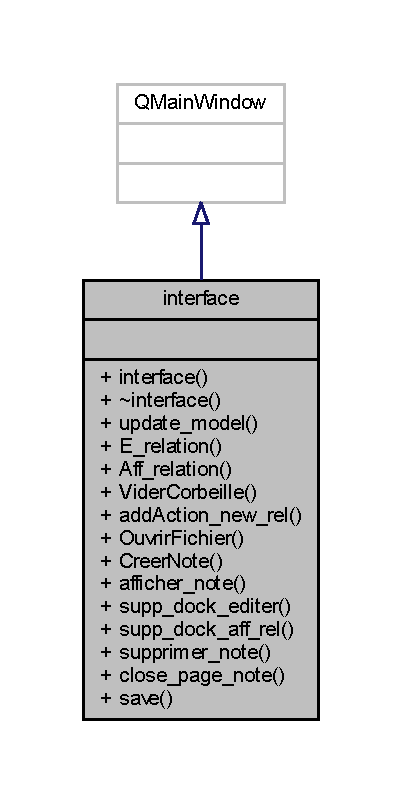
\includegraphics[width=193pt]{classinterface__inherit__graph}
\end{center}
\end{figure}


Collaboration diagram for interface\+:\nopagebreak
\begin{figure}[H]
\begin{center}
\leavevmode
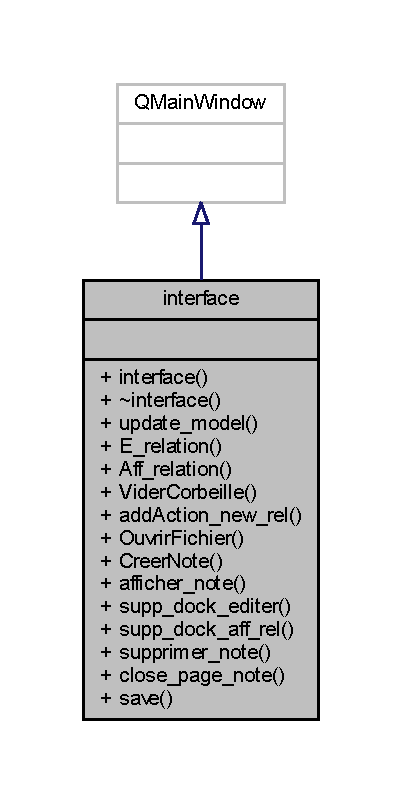
\includegraphics[width=193pt]{classinterface__coll__graph}
\end{center}
\end{figure}
\subsection*{Public Slots}
\begin{DoxyCompactItemize}
\item 
\mbox{\Hypertarget{classinterface_ac23ab5d301d541fecb1c92e214935fd1}\label{classinterface_ac23ab5d301d541fecb1c92e214935fd1}} 
void \hyperlink{classinterface_ac23ab5d301d541fecb1c92e214935fd1}{update\+\_\+model} ()
\begin{DoxyCompactList}\small\item\em envoi un signal de mis à jours à tous les docks. \end{DoxyCompactList}\item 
\mbox{\Hypertarget{classinterface_a65202c3659f8058ab91b3b01cf8f267f}\label{classinterface_a65202c3659f8058ab91b3b01cf8f267f}} 
void {\bfseries E\+\_\+relation} ()
\item 
void \hyperlink{classinterface_a287c8a46ece12a94540a190b96b911c9}{Aff\+\_\+relation} ()
\begin{DoxyCompactList}\small\item\em lance et connecte la fenetre de gestion des relations. \end{DoxyCompactList}\item 
void \hyperlink{classinterface_a430ee153cb2ea74b9103081d48cd61f3}{Vider\+Corbeille} ()
\begin{DoxyCompactList}\small\item\em Vide la corbeille. \end{DoxyCompactList}\item 
\mbox{\Hypertarget{classinterface_afda8f97b198f7d434cb1eb2d845dfefc}\label{classinterface_afda8f97b198f7d434cb1eb2d845dfefc}} 
void \hyperlink{classinterface_afda8f97b198f7d434cb1eb2d845dfefc}{add\+Action\+\_\+new\+\_\+rel} ()
\begin{DoxyCompactList}\small\item\em fonction outils, permettant de connecter, afficher l\textquotesingle{}action d\textquotesingle{}achiver une note a la page courante. \end{DoxyCompactList}\item 
\mbox{\Hypertarget{classinterface_af42d8f6426ad19ce13f1dd2ce9f519c1}\label{classinterface_af42d8f6426ad19ce13f1dd2ce9f519c1}} 
void \hyperlink{classinterface_af42d8f6426ad19ce13f1dd2ce9f519c1}{Ouvrir\+Fichier} ()
\begin{DoxyCompactList}\small\item\em Fenêtre permettant de selectionner/chargé un fichier de sauvegarde Met à jour le manager de note et les docks. \end{DoxyCompactList}\item 
void \hyperlink{classinterface_a23957135caad59d8850fe8e2cbee28a3}{Creer\+Note} ()
\begin{DoxyCompactList}\small\item\em Ouvre une fenetre de dialogue de type \hyperlink{class_creation___note}{Creation\+\_\+\+Note}, pour permettre la création d\textquotesingle{}une note. \end{DoxyCompactList}\item 
void \hyperlink{classinterface_a320051a7a36aa24f53b12df82649f15f}{afficher\+\_\+note} (Q\+String id, int i)
\begin{DoxyCompactList}\small\item\em slot qui permet l\textquotesingle{}ouverture d\textquotesingle{}une note. \end{DoxyCompactList}\item 
\mbox{\Hypertarget{classinterface_a3144306293774f567cbe90fa90cfd796}\label{classinterface_a3144306293774f567cbe90fa90cfd796}} 
void \hyperlink{classinterface_a3144306293774f567cbe90fa90cfd796}{supp\+\_\+dock\+\_\+editer} ()
\begin{DoxyCompactList}\small\item\em ferme le dock editer \end{DoxyCompactList}\item 
\mbox{\Hypertarget{classinterface_a1a6237ea46e9abd0662b8ec19c556f5e}\label{classinterface_a1a6237ea46e9abd0662b8ec19c556f5e}} 
void {\bfseries supp\+\_\+dock\+\_\+aff\+\_\+rel} ()
\item 
void \hyperlink{classinterface_aca23c755ba40ca8198010ff0487b22a8}{supprimer\+\_\+note} ()
\begin{DoxyCompactList}\small\item\em appelle la fenêtre de dialogue de suppression de note \end{DoxyCompactList}\item 
void \hyperlink{classinterface_abe2464522932a5d8ed76d1ba02c9d2c6}{close\+\_\+page\+\_\+note} ()
\begin{DoxyCompactList}\small\item\em Ferme la note en cours, si elle est bien encore ouverte. \end{DoxyCompactList}\item 
void \hyperlink{classinterface_a319f133949e2be97a203f725c3f1e565}{save} ()
\begin{DoxyCompactList}\small\item\em Permet de choisir/créer un fichier de sauvegarde. \end{DoxyCompactList}\end{DoxyCompactItemize}
\subsection*{Signals}
\begin{DoxyCompactItemize}
\item 
\mbox{\Hypertarget{classinterface_a300de30478e2e2616b61abad24bf319a}\label{classinterface_a300de30478e2e2616b61abad24bf319a}} 
void {\bfseries S\+\_\+update\+\_\+model} ()
\item 
\mbox{\Hypertarget{classinterface_a7d829b8bd407c58d27b0849f4891f155}\label{classinterface_a7d829b8bd407c58d27b0849f4891f155}} 
void {\bfseries L\+\_\+update\+\_\+model} ()
\item 
\mbox{\Hypertarget{classinterface_ad09217bb805eb4405dfc8d0b7cc6e547}\label{classinterface_ad09217bb805eb4405dfc8d0b7cc6e547}} 
void {\bfseries A\+\_\+update\+\_\+model} ()
\end{DoxyCompactItemize}
\subsection*{Public Member Functions}
\begin{DoxyCompactItemize}
\item 
\hyperlink{classinterface_a13e0ee4b9df1714d747d62ec46220c55}{interface} ()
\begin{DoxyCompactList}\small\item\em Constructeur de la classe interface Fenêtre principale de l\textquotesingle{}application, gére tous les docks, effectue la liason entre les docks, les widget, et les boites de dialogues. \end{DoxyCompactList}\item 
\hyperlink{classinterface_a8511f28c5bc5d3c24a24e9aaef4db502}{$\sim$interface} ()
\begin{DoxyCompactList}\small\item\em Ferme l\textquotesingle{}interface. \end{DoxyCompactList}\end{DoxyCompactItemize}


\subsection{Detailed Description}


Definition at line 71 of file interface.\+h.



\subsection{Constructor \& Destructor Documentation}
\mbox{\Hypertarget{classinterface_a13e0ee4b9df1714d747d62ec46220c55}\label{classinterface_a13e0ee4b9df1714d747d62ec46220c55}} 
\index{interface@{interface}!interface@{interface}}
\index{interface@{interface}!interface@{interface}}
\subsubsection{\texorpdfstring{interface()}{interface()}}
{\footnotesize\ttfamily interface\+::interface (\begin{DoxyParamCaption}{ }\end{DoxyParamCaption})}



Constructeur de la classe interface Fenêtre principale de l\textquotesingle{}application, gére tous les docks, effectue la liason entre les docks, les widget, et les boites de dialogues. 


\begin{DoxyParams}{Parameters}
{\em } & \\
\hline
\end{DoxyParams}


Definition at line 28 of file interface.\+cpp.

Here is the call graph for this function\+:\nopagebreak
\begin{figure}[H]
\begin{center}
\leavevmode
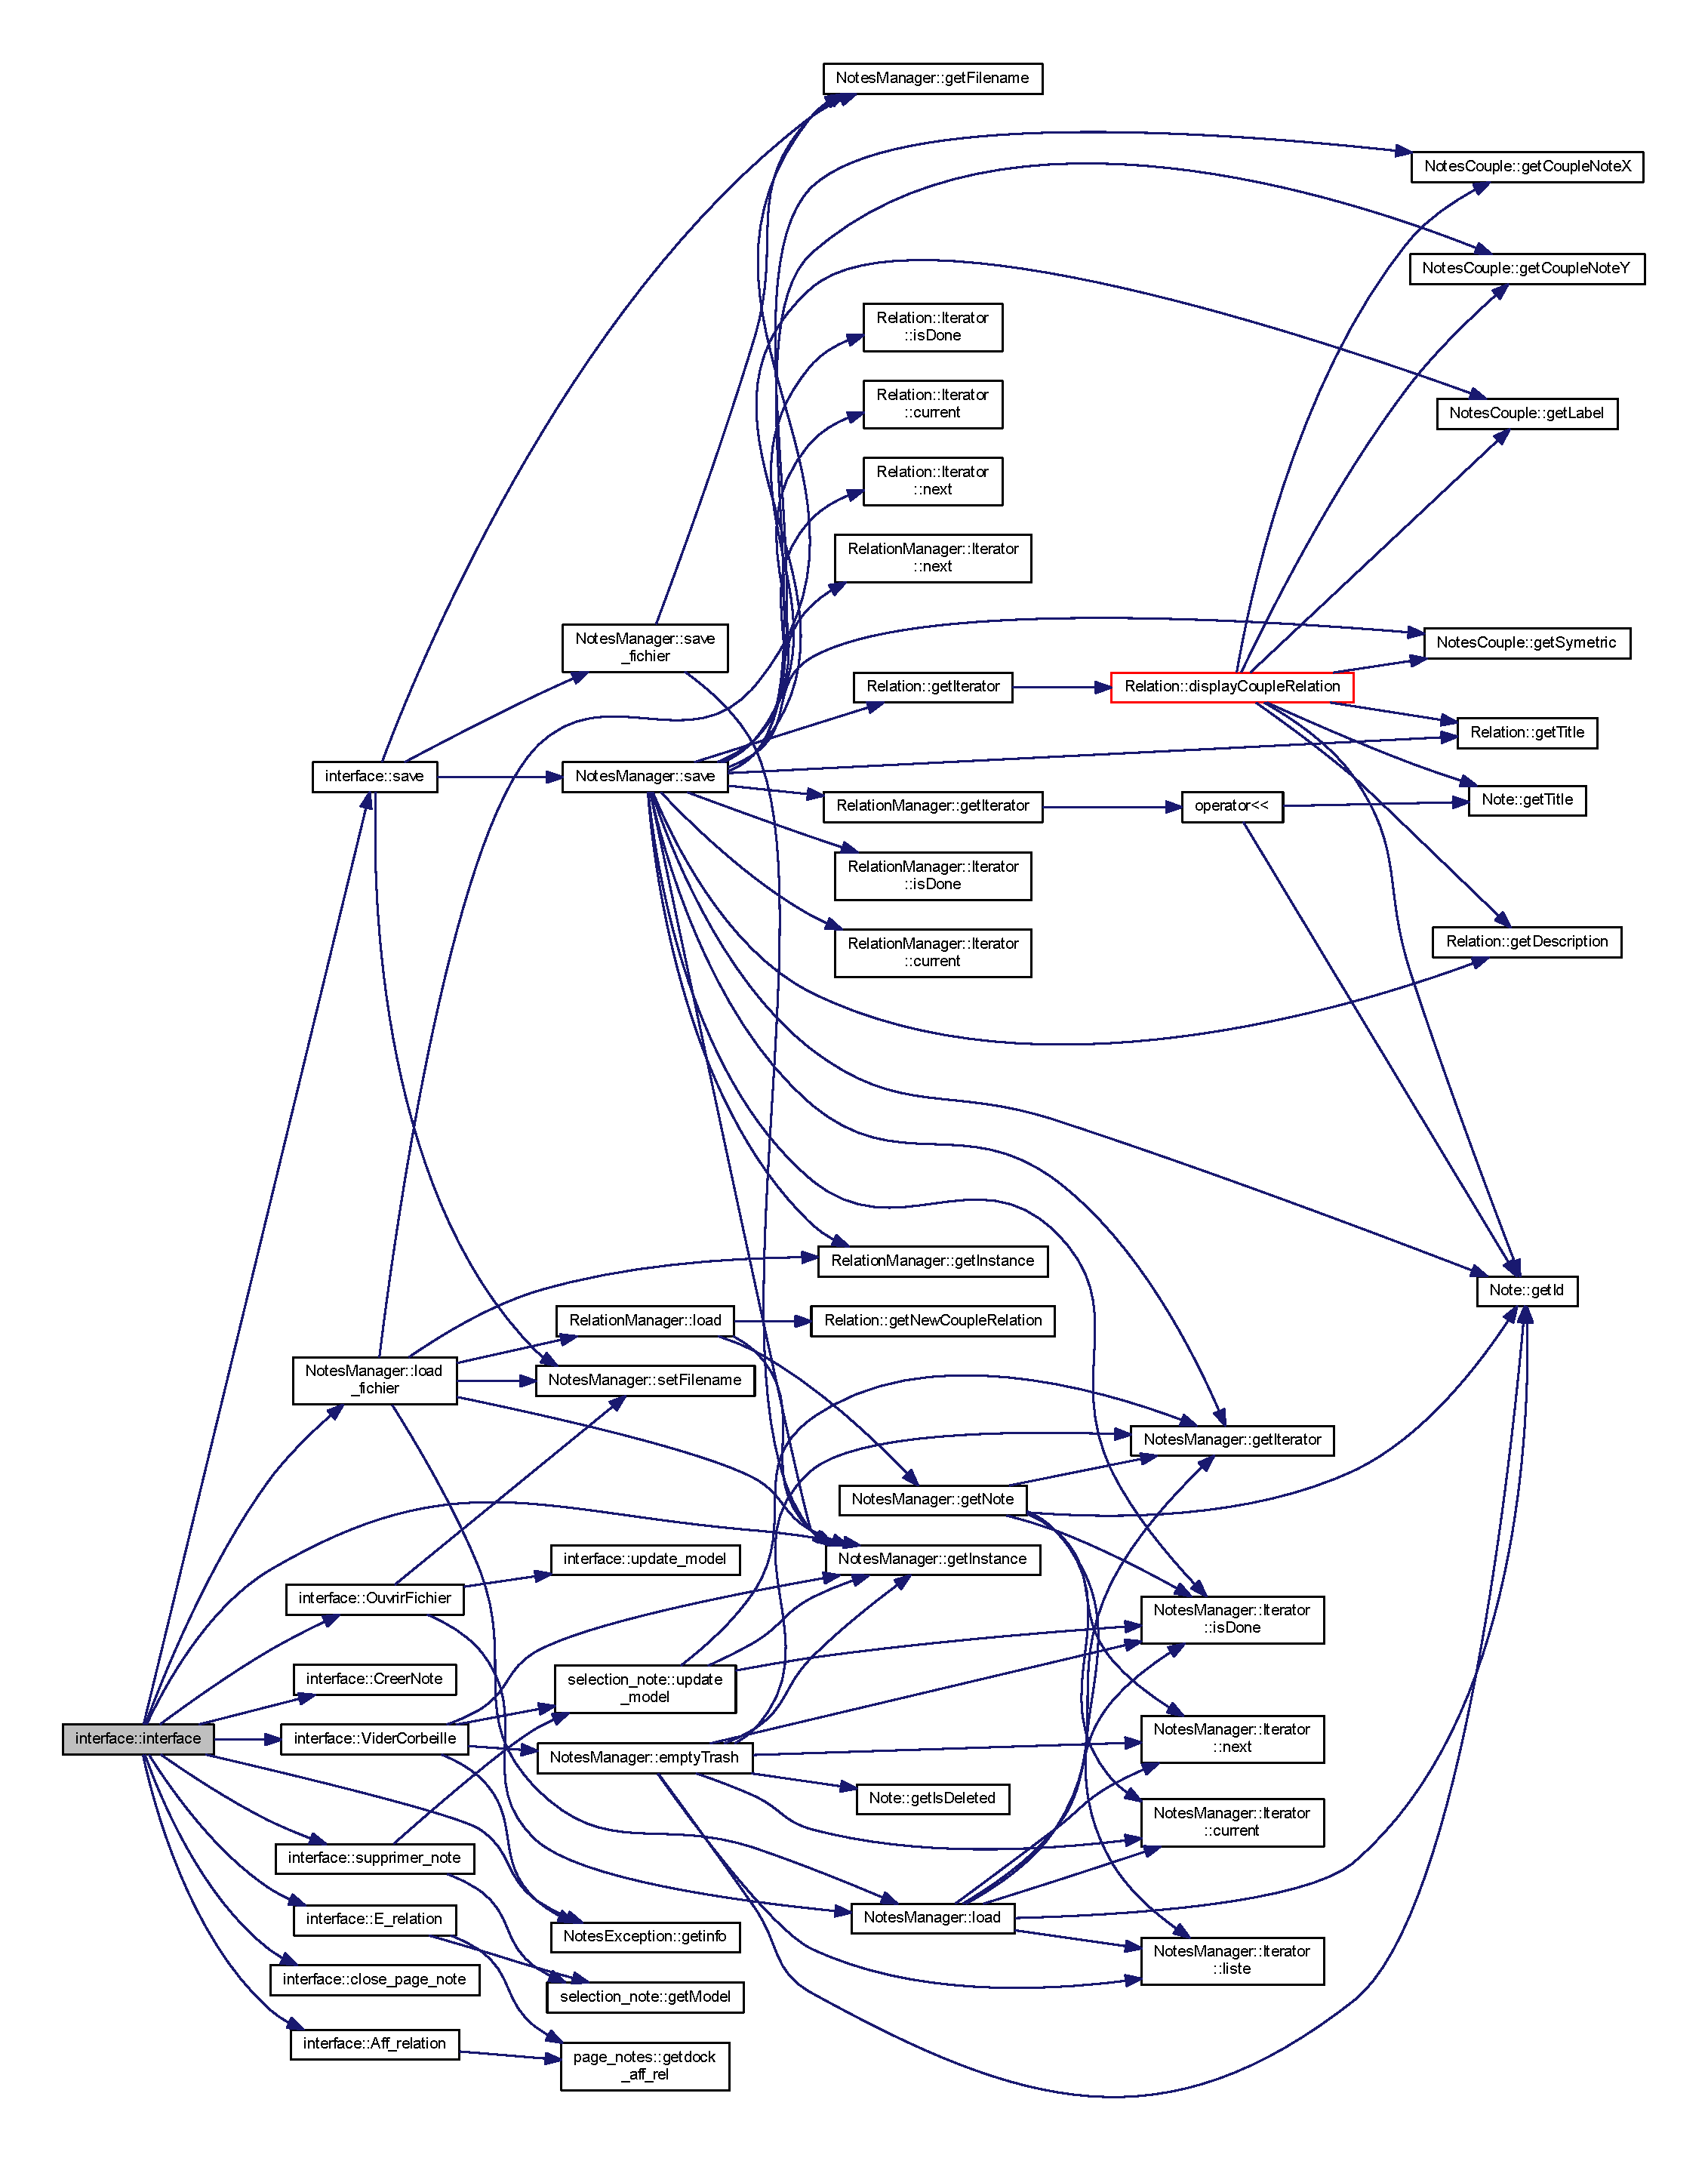
\includegraphics[width=350pt]{classinterface_a13e0ee4b9df1714d747d62ec46220c55_cgraph}
\end{center}
\end{figure}
\mbox{\Hypertarget{classinterface_a8511f28c5bc5d3c24a24e9aaef4db502}\label{classinterface_a8511f28c5bc5d3c24a24e9aaef4db502}} 
\index{interface@{interface}!````~interface@{$\sim$interface}}
\index{````~interface@{$\sim$interface}!interface@{interface}}
\subsubsection{\texorpdfstring{$\sim$interface()}{~interface()}}
{\footnotesize\ttfamily interface\+::$\sim$interface (\begin{DoxyParamCaption}{ }\end{DoxyParamCaption})}



Ferme l\textquotesingle{}interface. 

Vide la corbeille puis effectuer une sauvegarde automatique si il y a un fichier de sauvegarde référencer. 

Definition at line 123 of file interface.\+cpp.

Here is the call graph for this function\+:\nopagebreak
\begin{figure}[H]
\begin{center}
\leavevmode
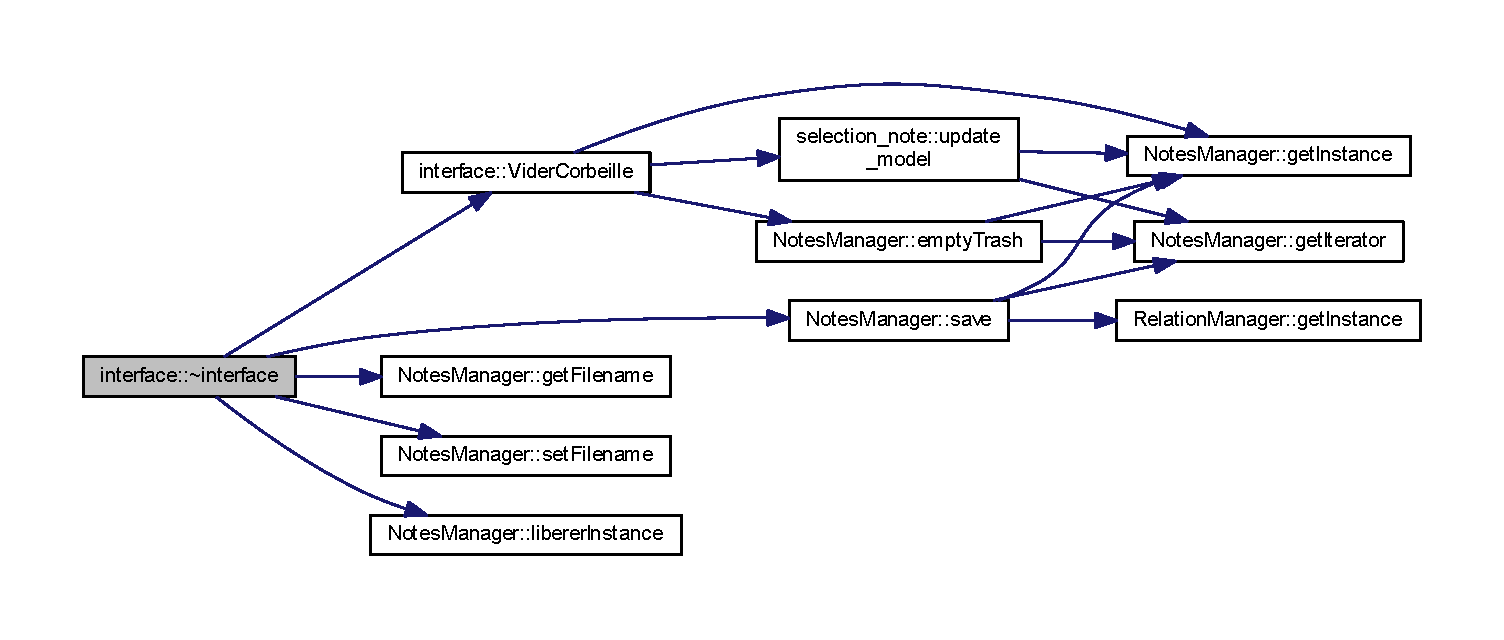
\includegraphics[width=350pt]{classinterface_a8511f28c5bc5d3c24a24e9aaef4db502_cgraph}
\end{center}
\end{figure}


\subsection{Member Function Documentation}
\mbox{\Hypertarget{classinterface_a287c8a46ece12a94540a190b96b911c9}\label{classinterface_a287c8a46ece12a94540a190b96b911c9}} 
\index{interface@{interface}!Aff\+\_\+relation@{Aff\+\_\+relation}}
\index{Aff\+\_\+relation@{Aff\+\_\+relation}!interface@{interface}}
\subsubsection{\texorpdfstring{Aff\+\_\+relation}{Aff\_relation}}
{\footnotesize\ttfamily interface\+::\+Aff\+\_\+relation (\begin{DoxyParamCaption}{ }\end{DoxyParamCaption})\hspace{0.3cm}{\ttfamily [inline]}, {\ttfamily [slot]}}



lance et connecte la fenetre de gestion des relations. 

connecte cette dernière avec le dock relation sur la page principale 

Definition at line 146 of file interface.\+h.

Here is the caller graph for this function\+:\nopagebreak
\begin{figure}[H]
\begin{center}
\leavevmode
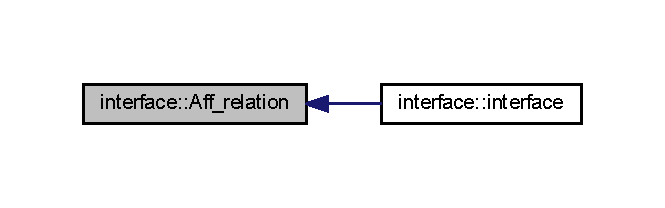
\includegraphics[width=319pt]{classinterface_a287c8a46ece12a94540a190b96b911c9_icgraph}
\end{center}
\end{figure}
\mbox{\Hypertarget{classinterface_a320051a7a36aa24f53b12df82649f15f}\label{classinterface_a320051a7a36aa24f53b12df82649f15f}} 
\index{interface@{interface}!afficher\+\_\+note@{afficher\+\_\+note}}
\index{afficher\+\_\+note@{afficher\+\_\+note}!interface@{interface}}
\subsubsection{\texorpdfstring{afficher\+\_\+note}{afficher\_note}}
{\footnotesize\ttfamily void interface\+::afficher\+\_\+note (\begin{DoxyParamCaption}\item[{Q\+String}]{id,  }\item[{int}]{i }\end{DoxyParamCaption})\hspace{0.3cm}{\ttfamily [slot]}}



slot qui permet l\textquotesingle{}ouverture d\textquotesingle{}une note. 

\hyperlink{classinterface_a320051a7a36aa24f53b12df82649f15f}{interface\+::afficher\+\_\+note} 
\begin{DoxyParams}{Parameters}
{\em id} & \\
\hline
{\em i} & \\
\hline
\end{DoxyParams}
Elle vérifie si une note était déjà ouverte avant \+: la ferme, restaure la note, supprime le pointeur sur la note courante essaye d\textquotesingle{}ouvrir la versions sélectionné \+: connecte cette dernière avec l\textquotesingle{}interface si il est impossible d\textquotesingle{}ouvrir la note, on affiche la page d\textquotesingle{}acceuil. 

Definition at line 402 of file interface.\+cpp.

Here is the call graph for this function\+:\nopagebreak
\begin{figure}[H]
\begin{center}
\leavevmode
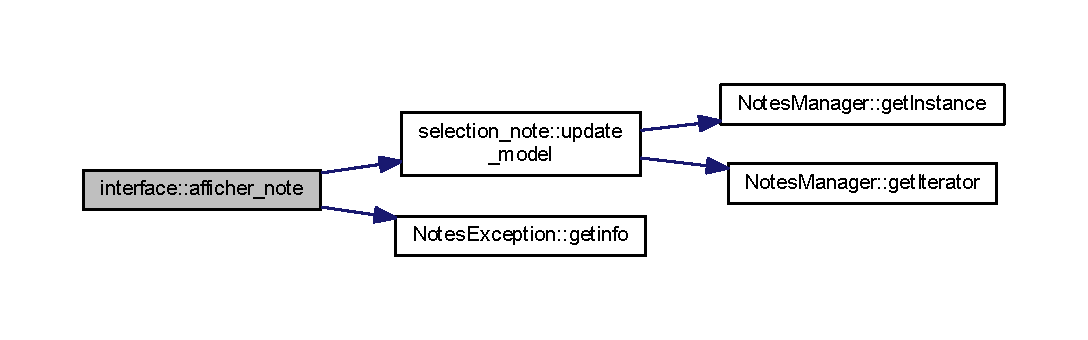
\includegraphics[width=350pt]{classinterface_a320051a7a36aa24f53b12df82649f15f_cgraph}
\end{center}
\end{figure}
Here is the caller graph for this function\+:\nopagebreak
\begin{figure}[H]
\begin{center}
\leavevmode
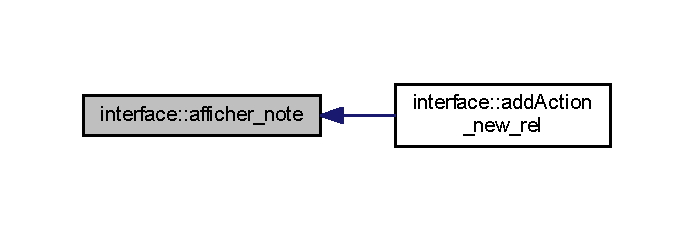
\includegraphics[width=333pt]{classinterface_a320051a7a36aa24f53b12df82649f15f_icgraph}
\end{center}
\end{figure}
\mbox{\Hypertarget{classinterface_abe2464522932a5d8ed76d1ba02c9d2c6}\label{classinterface_abe2464522932a5d8ed76d1ba02c9d2c6}} 
\index{interface@{interface}!close\+\_\+page\+\_\+note@{close\+\_\+page\+\_\+note}}
\index{close\+\_\+page\+\_\+note@{close\+\_\+page\+\_\+note}!interface@{interface}}
\subsubsection{\texorpdfstring{close\+\_\+page\+\_\+note}{close\_page\_note}}
{\footnotesize\ttfamily void interface\+::close\+\_\+page\+\_\+note (\begin{DoxyParamCaption}{ }\end{DoxyParamCaption})\hspace{0.3cm}{\ttfamily [slot]}}



Ferme la note en cours, si elle est bien encore ouverte. 

Action déclenché lorqu\textquotesingle{}on click sur le bouton de fermeture d\textquotesingle{}une note 

Definition at line 440 of file interface.\+cpp.

Here is the caller graph for this function\+:\nopagebreak
\begin{figure}[H]
\begin{center}
\leavevmode
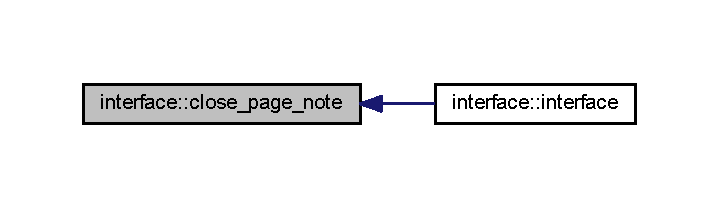
\includegraphics[width=345pt]{classinterface_abe2464522932a5d8ed76d1ba02c9d2c6_icgraph}
\end{center}
\end{figure}
\mbox{\Hypertarget{classinterface_a23957135caad59d8850fe8e2cbee28a3}\label{classinterface_a23957135caad59d8850fe8e2cbee28a3}} 
\index{interface@{interface}!Creer\+Note@{Creer\+Note}}
\index{Creer\+Note@{Creer\+Note}!interface@{interface}}
\subsubsection{\texorpdfstring{Creer\+Note}{CreerNote}}
{\footnotesize\ttfamily void interface\+::\+Creer\+Note (\begin{DoxyParamCaption}{ }\end{DoxyParamCaption})\hspace{0.3cm}{\ttfamily [slot]}}



Ouvre une fenetre de dialogue de type \hyperlink{class_creation___note}{Creation\+\_\+\+Note}, pour permettre la création d\textquotesingle{}une note. 

Une fois la note créer, le dock de note actif est mis à jour sont mis à jours 

Definition at line 299 of file interface.\+cpp.

Here is the caller graph for this function\+:\nopagebreak
\begin{figure}[H]
\begin{center}
\leavevmode
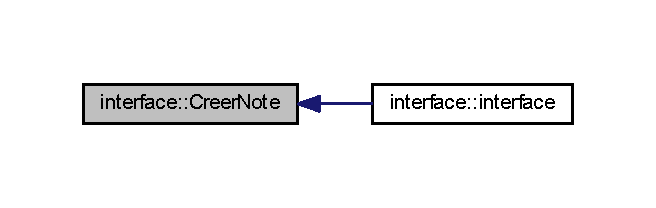
\includegraphics[width=315pt]{classinterface_a23957135caad59d8850fe8e2cbee28a3_icgraph}
\end{center}
\end{figure}
\mbox{\Hypertarget{classinterface_a319f133949e2be97a203f725c3f1e565}\label{classinterface_a319f133949e2be97a203f725c3f1e565}} 
\index{interface@{interface}!save@{save}}
\index{save@{save}!interface@{interface}}
\subsubsection{\texorpdfstring{save}{save}}
{\footnotesize\ttfamily void interface\+::save (\begin{DoxyParamCaption}{ }\end{DoxyParamCaption})\hspace{0.3cm}{\ttfamily [slot]}}



Permet de choisir/créer un fichier de sauvegarde. 

En cas de fichier invalide, la sauvegarde n\textquotesingle{}est pas effectué, et un signal critique est envoyé à l\textquotesingle{}utilisateur 
\begin{DoxyParams}{Parameters}
{\em } & \\
\hline
\end{DoxyParams}


Definition at line 258 of file interface.\+cpp.

Here is the call graph for this function\+:\nopagebreak
\begin{figure}[H]
\begin{center}
\leavevmode
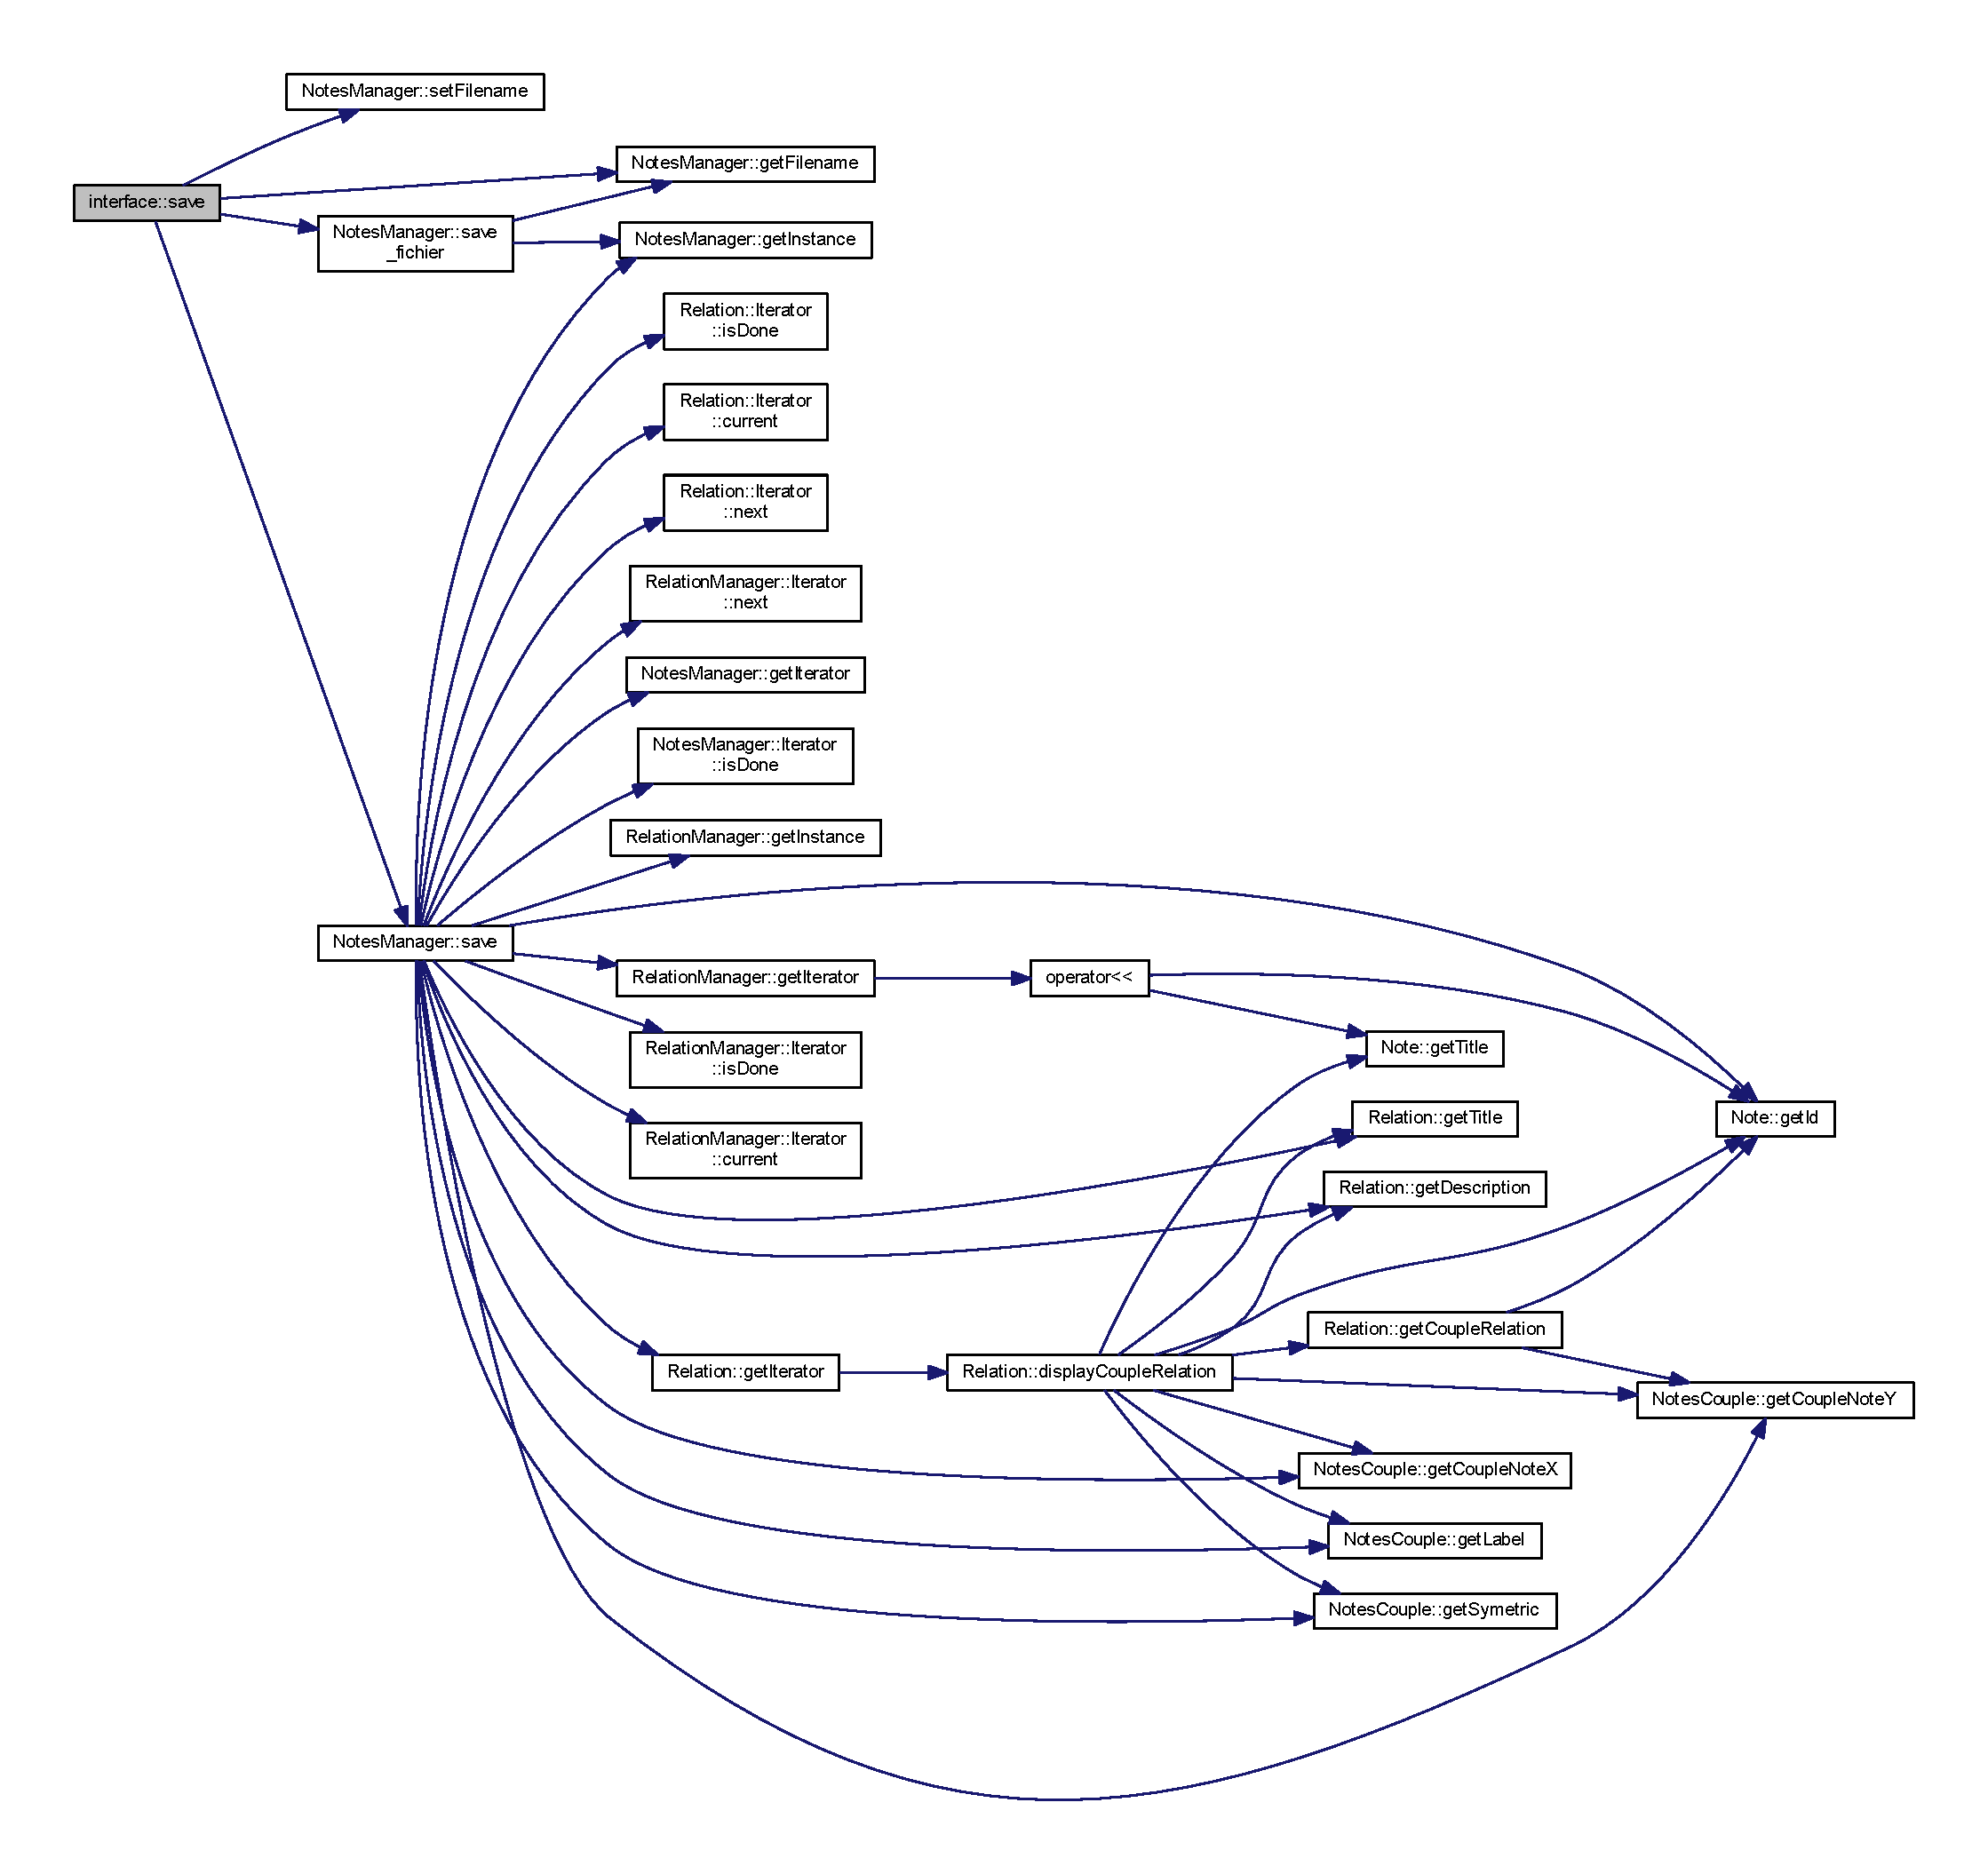
\includegraphics[width=350pt]{classinterface_a319f133949e2be97a203f725c3f1e565_cgraph}
\end{center}
\end{figure}
Here is the caller graph for this function\+:\nopagebreak
\begin{figure}[H]
\begin{center}
\leavevmode
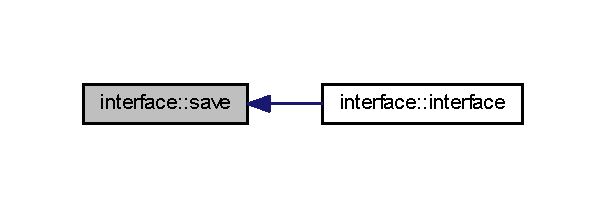
\includegraphics[width=291pt]{classinterface_a319f133949e2be97a203f725c3f1e565_icgraph}
\end{center}
\end{figure}
\mbox{\Hypertarget{classinterface_aca23c755ba40ca8198010ff0487b22a8}\label{classinterface_aca23c755ba40ca8198010ff0487b22a8}} 
\index{interface@{interface}!supprimer\+\_\+note@{supprimer\+\_\+note}}
\index{supprimer\+\_\+note@{supprimer\+\_\+note}!interface@{interface}}
\subsubsection{\texorpdfstring{supprimer\+\_\+note}{supprimer\_note}}
{\footnotesize\ttfamily interface\+::supprimer\+\_\+note (\begin{DoxyParamCaption}{ }\end{DoxyParamCaption})\hspace{0.3cm}{\ttfamily [inline]}, {\ttfamily [slot]}}



appelle la fenêtre de dialogue de suppression de note 

Ferme la page en cours, et mes à jours les docks 

Definition at line 195 of file interface.\+h.

Here is the call graph for this function\+:\nopagebreak
\begin{figure}[H]
\begin{center}
\leavevmode
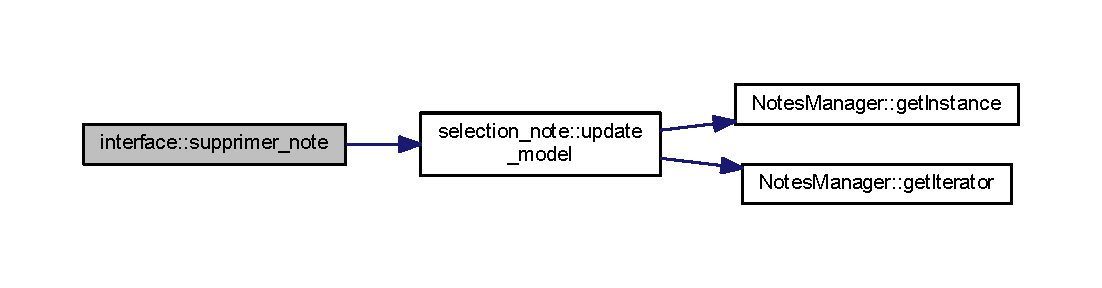
\includegraphics[width=350pt]{classinterface_aca23c755ba40ca8198010ff0487b22a8_cgraph}
\end{center}
\end{figure}
Here is the caller graph for this function\+:\nopagebreak
\begin{figure}[H]
\begin{center}
\leavevmode
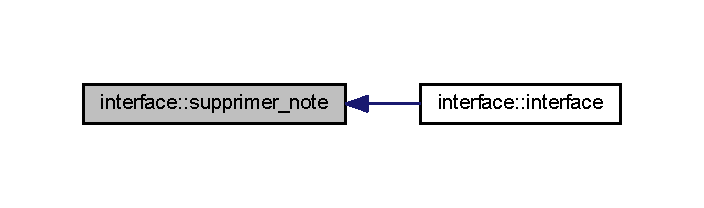
\includegraphics[width=338pt]{classinterface_aca23c755ba40ca8198010ff0487b22a8_icgraph}
\end{center}
\end{figure}
\mbox{\Hypertarget{classinterface_a430ee153cb2ea74b9103081d48cd61f3}\label{classinterface_a430ee153cb2ea74b9103081d48cd61f3}} 
\index{interface@{interface}!Vider\+Corbeille@{Vider\+Corbeille}}
\index{Vider\+Corbeille@{Vider\+Corbeille}!interface@{interface}}
\subsubsection{\texorpdfstring{Vider\+Corbeille}{ViderCorbeille}}
{\footnotesize\ttfamily interface\+::\+Vider\+Corbeille (\begin{DoxyParamCaption}{ }\end{DoxyParamCaption})\hspace{0.3cm}{\ttfamily [inline]}, {\ttfamily [slot]}}



Vide la corbeille. 

ferme la page en cours, et appelle empty\+Trash, une methode du manager mes à jours les docks 

Definition at line 159 of file interface.\+h.

Here is the call graph for this function\+:\nopagebreak
\begin{figure}[H]
\begin{center}
\leavevmode
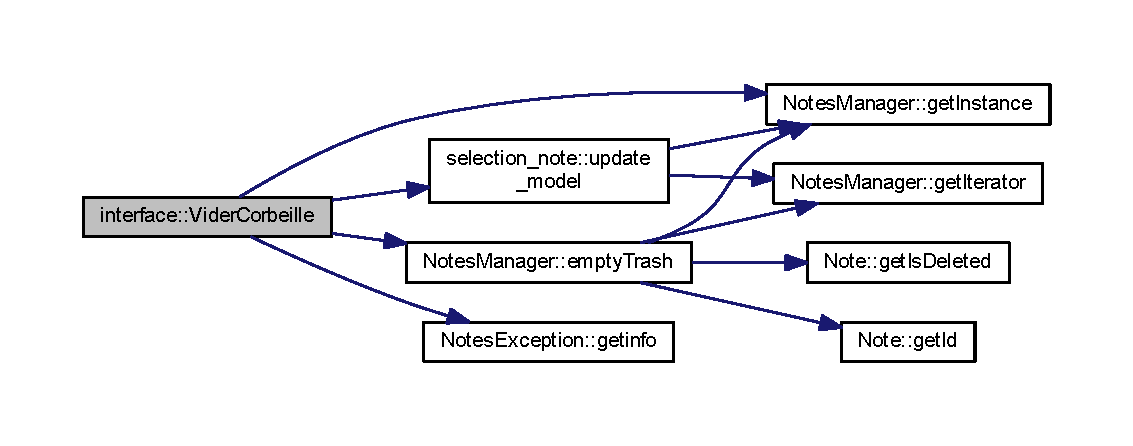
\includegraphics[width=350pt]{classinterface_a430ee153cb2ea74b9103081d48cd61f3_cgraph}
\end{center}
\end{figure}
Here is the caller graph for this function\+:\nopagebreak
\begin{figure}[H]
\begin{center}
\leavevmode
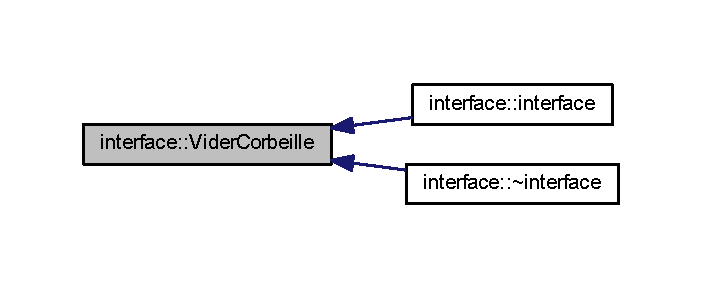
\includegraphics[width=337pt]{classinterface_a430ee153cb2ea74b9103081d48cd61f3_icgraph}
\end{center}
\end{figure}


The documentation for this class was generated from the following files\+:\begin{DoxyCompactItemize}
\item 
O\+L13/\hyperlink{interface_8h}{interface.\+h}\item 
O\+L13/\hyperlink{interface_8cpp}{interface.\+cpp}\end{DoxyCompactItemize}

\hypertarget{class_relation_manager_1_1_iterator}{}\section{Relation\+Manager\+:\+:Iterator Class Reference}
\label{class_relation_manager_1_1_iterator}\index{Relation\+Manager\+::\+Iterator@{Relation\+Manager\+::\+Iterator}}


Collaboration diagram for Relation\+Manager\+:\+:Iterator\+:\nopagebreak
\begin{figure}[H]
\begin{center}
\leavevmode
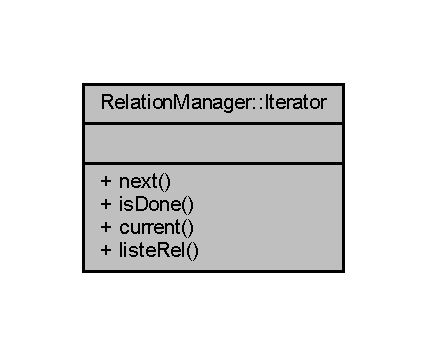
\includegraphics[width=205pt]{class_relation_manager_1_1_iterator__coll__graph}
\end{center}
\end{figure}
\subsection*{Public Member Functions}
\begin{DoxyCompactItemize}
\item 
\mbox{\Hypertarget{class_relation_manager_1_1_iterator_a4deab2fdd2f7b70242ecbfab9d3d1552}\label{class_relation_manager_1_1_iterator_a4deab2fdd2f7b70242ecbfab9d3d1552}} 
void {\bfseries next} ()
\item 
\mbox{\Hypertarget{class_relation_manager_1_1_iterator_a5e9588417d8c6dc8ce1285612dff7840}\label{class_relation_manager_1_1_iterator_a5e9588417d8c6dc8ce1285612dff7840}} 
bool {\bfseries is\+Done} () const
\item 
\mbox{\Hypertarget{class_relation_manager_1_1_iterator_ad3f5e514500480f65dc9b14d1aae358f}\label{class_relation_manager_1_1_iterator_ad3f5e514500480f65dc9b14d1aae358f}} 
\hyperlink{class_relation}{Relation} \& {\bfseries current} () const
\item 
\mbox{\Hypertarget{class_relation_manager_1_1_iterator_a017175bf4f16360c5b2ee5d8fd534d22}\label{class_relation_manager_1_1_iterator_a017175bf4f16360c5b2ee5d8fd534d22}} 
\hyperlink{class_relation}{Relation} $\ast$ {\bfseries liste\+Rel} ()
\end{DoxyCompactItemize}
\subsection*{Friends}
\begin{DoxyCompactItemize}
\item 
\mbox{\Hypertarget{class_relation_manager_1_1_iterator_a55fae9c2e48742dd0a8596e6d8721775}\label{class_relation_manager_1_1_iterator_a55fae9c2e48742dd0a8596e6d8721775}} 
class {\bfseries Relation\+Manager}
\end{DoxyCompactItemize}


\subsection{Detailed Description}


Definition at line 190 of file manager.\+h.



The documentation for this class was generated from the following file\+:\begin{DoxyCompactItemize}
\item 
O\+L13/\hyperlink{manager_8h}{manager.\+h}\end{DoxyCompactItemize}

\hypertarget{class_relation_1_1_iterator}{}\section{Relation\+:\+:Iterator Class Reference}
\label{class_relation_1_1_iterator}\index{Relation\+::\+Iterator@{Relation\+::\+Iterator}}


Collaboration diagram for Relation\+:\+:Iterator\+:\nopagebreak
\begin{figure}[H]
\begin{center}
\leavevmode
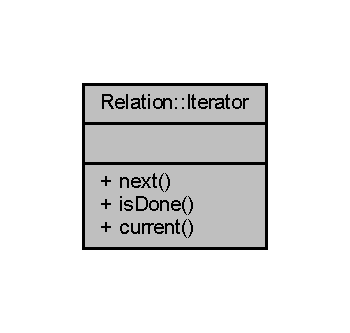
\includegraphics[width=168pt]{class_relation_1_1_iterator__coll__graph}
\end{center}
\end{figure}
\subsection*{Public Member Functions}
\begin{DoxyCompactItemize}
\item 
\mbox{\Hypertarget{class_relation_1_1_iterator_a567ce85dbb1ec314899e495970945116}\label{class_relation_1_1_iterator_a567ce85dbb1ec314899e495970945116}} 
void \hyperlink{class_relation_1_1_iterator_a567ce85dbb1ec314899e495970945116}{next} ()
\begin{DoxyCompactList}\small\item\em Incrémentation de l\textquotesingle{}itérateur. \end{DoxyCompactList}\item 
bool \hyperlink{class_relation_1_1_iterator_ace43327cf3c6e78a3446150a9c65c871}{is\+Done} () const
\begin{DoxyCompactList}\small\item\em Vérifie si on a terminé d\textquotesingle{}itérer. \end{DoxyCompactList}\item 
\hyperlink{class_notes_couple}{Notes\+Couple} \& \hyperlink{class_relation_1_1_iterator_ae790f3731aad304b3930fb23fa5b9c7c}{current} () const
\begin{DoxyCompactList}\small\item\em Renvoi l\textquotesingle{}élément courant. \end{DoxyCompactList}\end{DoxyCompactItemize}
\subsection*{Friends}
\begin{DoxyCompactItemize}
\item 
\mbox{\Hypertarget{class_relation_1_1_iterator_a7ee004262f27f8c916688911a71e3aa1}\label{class_relation_1_1_iterator_a7ee004262f27f8c916688911a71e3aa1}} 
class {\bfseries Relation}
\end{DoxyCompactItemize}


\subsection{Detailed Description}


Definition at line 145 of file relations.\+h.



\subsection{Member Function Documentation}
\mbox{\Hypertarget{class_relation_1_1_iterator_ae790f3731aad304b3930fb23fa5b9c7c}\label{class_relation_1_1_iterator_ae790f3731aad304b3930fb23fa5b9c7c}} 
\index{Relation\+::\+Iterator@{Relation\+::\+Iterator}!current@{current}}
\index{current@{current}!Relation\+::\+Iterator@{Relation\+::\+Iterator}}
\subsubsection{\texorpdfstring{current()}{current()}}
{\footnotesize\ttfamily Relation\+::\+Iterator\+::current (\begin{DoxyParamCaption}{ }\end{DoxyParamCaption}) const\hspace{0.3cm}{\ttfamily [inline]}}



Renvoi l\textquotesingle{}élément courant. 

\begin{DoxyReturn}{Returns}
Notes\+Couples\& 
\end{DoxyReturn}


Definition at line 178 of file relations.\+h.

Here is the caller graph for this function\+:\nopagebreak
\begin{figure}[H]
\begin{center}
\leavevmode
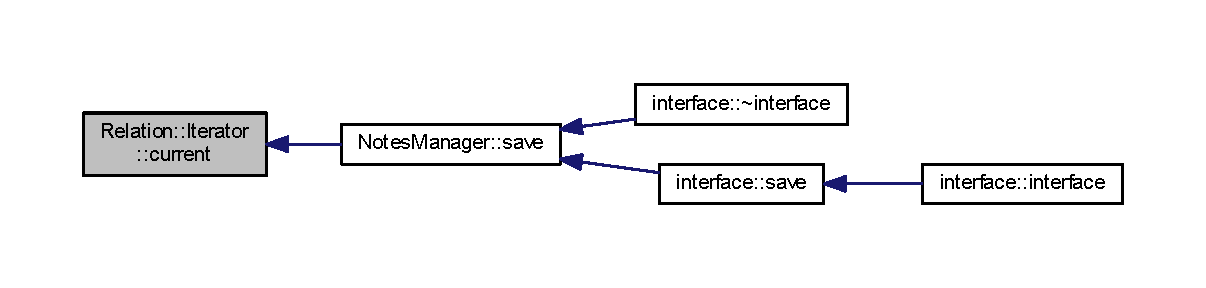
\includegraphics[width=350pt]{class_relation_1_1_iterator_ae790f3731aad304b3930fb23fa5b9c7c_icgraph}
\end{center}
\end{figure}
\mbox{\Hypertarget{class_relation_1_1_iterator_ace43327cf3c6e78a3446150a9c65c871}\label{class_relation_1_1_iterator_ace43327cf3c6e78a3446150a9c65c871}} 
\index{Relation\+::\+Iterator@{Relation\+::\+Iterator}!is\+Done@{is\+Done}}
\index{is\+Done@{is\+Done}!Relation\+::\+Iterator@{Relation\+::\+Iterator}}
\subsubsection{\texorpdfstring{is\+Done()}{isDone()}}
{\footnotesize\ttfamily Relation\+::\+Iterator\+::is\+Done (\begin{DoxyParamCaption}{ }\end{DoxyParamCaption}) const\hspace{0.3cm}{\ttfamily [inline]}}



Vérifie si on a terminé d\textquotesingle{}itérer. 

\begin{DoxyReturn}{Returns}
bool 
\end{DoxyReturn}


Definition at line 172 of file relations.\+h.

Here is the caller graph for this function\+:\nopagebreak
\begin{figure}[H]
\begin{center}
\leavevmode
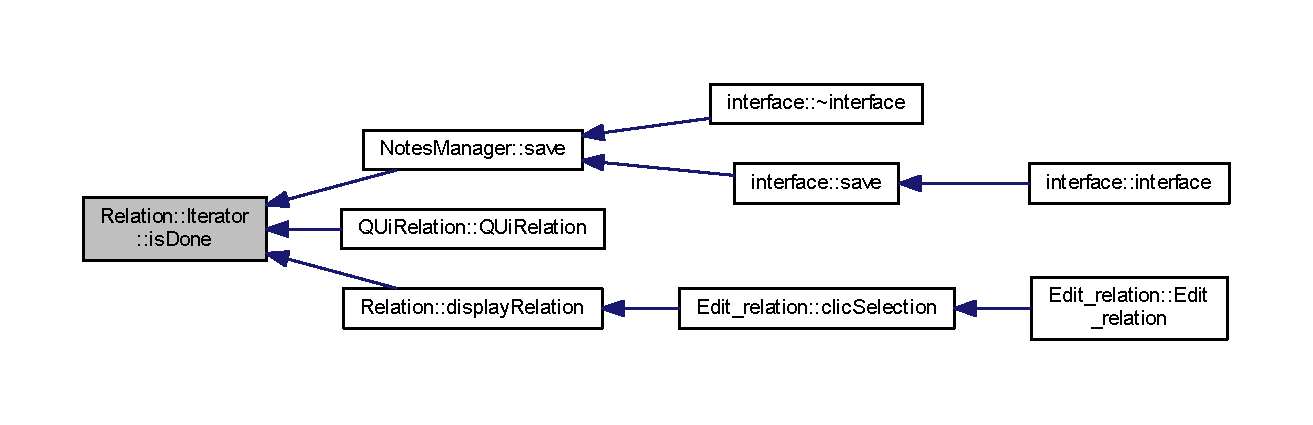
\includegraphics[width=350pt]{class_relation_1_1_iterator_ace43327cf3c6e78a3446150a9c65c871_icgraph}
\end{center}
\end{figure}


The documentation for this class was generated from the following file\+:\begin{DoxyCompactItemize}
\item 
O\+L13/\hyperlink{relations_8h}{relations.\+h}\end{DoxyCompactItemize}

\hypertarget{class_notes_manager_1_1_iterator}{}\section{Notes\+Manager\+:\+:Iterator Class Reference}
\label{class_notes_manager_1_1_iterator}\index{Notes\+Manager\+::\+Iterator@{Notes\+Manager\+::\+Iterator}}


Collaboration diagram for Notes\+Manager\+:\+:Iterator\+:\nopagebreak
\begin{figure}[H]
\begin{center}
\leavevmode
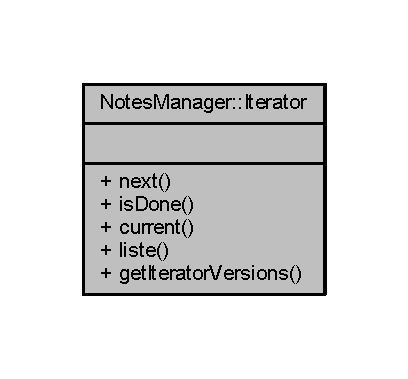
\includegraphics[width=196pt]{class_notes_manager_1_1_iterator__coll__graph}
\end{center}
\end{figure}
\subsection*{Public Member Functions}
\begin{DoxyCompactItemize}
\item 
\mbox{\Hypertarget{class_notes_manager_1_1_iterator_a4a6d6c9d3120acf8052728c0212b5ccd}\label{class_notes_manager_1_1_iterator_a4a6d6c9d3120acf8052728c0212b5ccd}} 
void \hyperlink{class_notes_manager_1_1_iterator_a4a6d6c9d3120acf8052728c0212b5ccd}{next} ()
\begin{DoxyCompactList}\small\item\em Incrémentation de l\textquotesingle{}itérateur. \end{DoxyCompactList}\item 
bool \hyperlink{class_notes_manager_1_1_iterator_a09b30631af5b7627b2b5a655a8ac450d}{is\+Done} () const
\begin{DoxyCompactList}\small\item\em Vérifie si l\textquotesingle{}itérateur est arrivé à la fin de la liste. \end{DoxyCompactList}\item 
\hyperlink{class_note}{Note} \& \hyperlink{class_notes_manager_1_1_iterator_a4fd73444f2edd5f196d7b950527f5a90}{current} () const
\begin{DoxyCompactList}\small\item\em Retourne la dernière version de la note courante. \end{DoxyCompactList}\item 
Q\+List$<$ \hyperlink{class_note}{Note} $\ast$ $>$ $\ast$ \hyperlink{class_notes_manager_1_1_iterator_a99e3eb098c3b5c7b3041731d10a18c88}{liste} ()
\begin{DoxyCompactList}\small\item\em Retourne la liste des toutes les versions de la note courante. \end{DoxyCompactList}\item 
Q\+List$<$ \hyperlink{class_note}{Note} $\ast$ $>$\+::iterator \hyperlink{class_notes_manager_1_1_iterator_a09a650ca2eeca614a4129ed5e1795e96}{get\+Iterator\+Versions} ()
\begin{DoxyCompactList}\small\item\em Renvoie un itérateur sur les versions de la note courante. \end{DoxyCompactList}\end{DoxyCompactItemize}
\subsection*{Friends}
\begin{DoxyCompactItemize}
\item 
\mbox{\Hypertarget{class_notes_manager_1_1_iterator_a017a5144e8cfa6087305055ab968ef41}\label{class_notes_manager_1_1_iterator_a017a5144e8cfa6087305055ab968ef41}} 
class {\bfseries Notes\+Manager}
\end{DoxyCompactItemize}


\subsection{Detailed Description}


Definition at line 139 of file manager.\+h.



\subsection{Member Function Documentation}
\mbox{\Hypertarget{class_notes_manager_1_1_iterator_a4fd73444f2edd5f196d7b950527f5a90}\label{class_notes_manager_1_1_iterator_a4fd73444f2edd5f196d7b950527f5a90}} 
\index{Notes\+Manager\+::\+Iterator@{Notes\+Manager\+::\+Iterator}!current@{current}}
\index{current@{current}!Notes\+Manager\+::\+Iterator@{Notes\+Manager\+::\+Iterator}}
\subsubsection{\texorpdfstring{current()}{current()}}
{\footnotesize\ttfamily Notes\+Manager\+::\+Iterator\+::current (\begin{DoxyParamCaption}{ }\end{DoxyParamCaption}) const\hspace{0.3cm}{\ttfamily [inline]}}



Retourne la dernière version de la note courante. 

\begin{DoxyReturn}{Returns}
\hyperlink{class_note}{Note}\& 
\end{DoxyReturn}


Definition at line 175 of file manager.\+h.

Here is the caller graph for this function\+:
\nopagebreak
\begin{figure}[H]
\begin{center}
\leavevmode
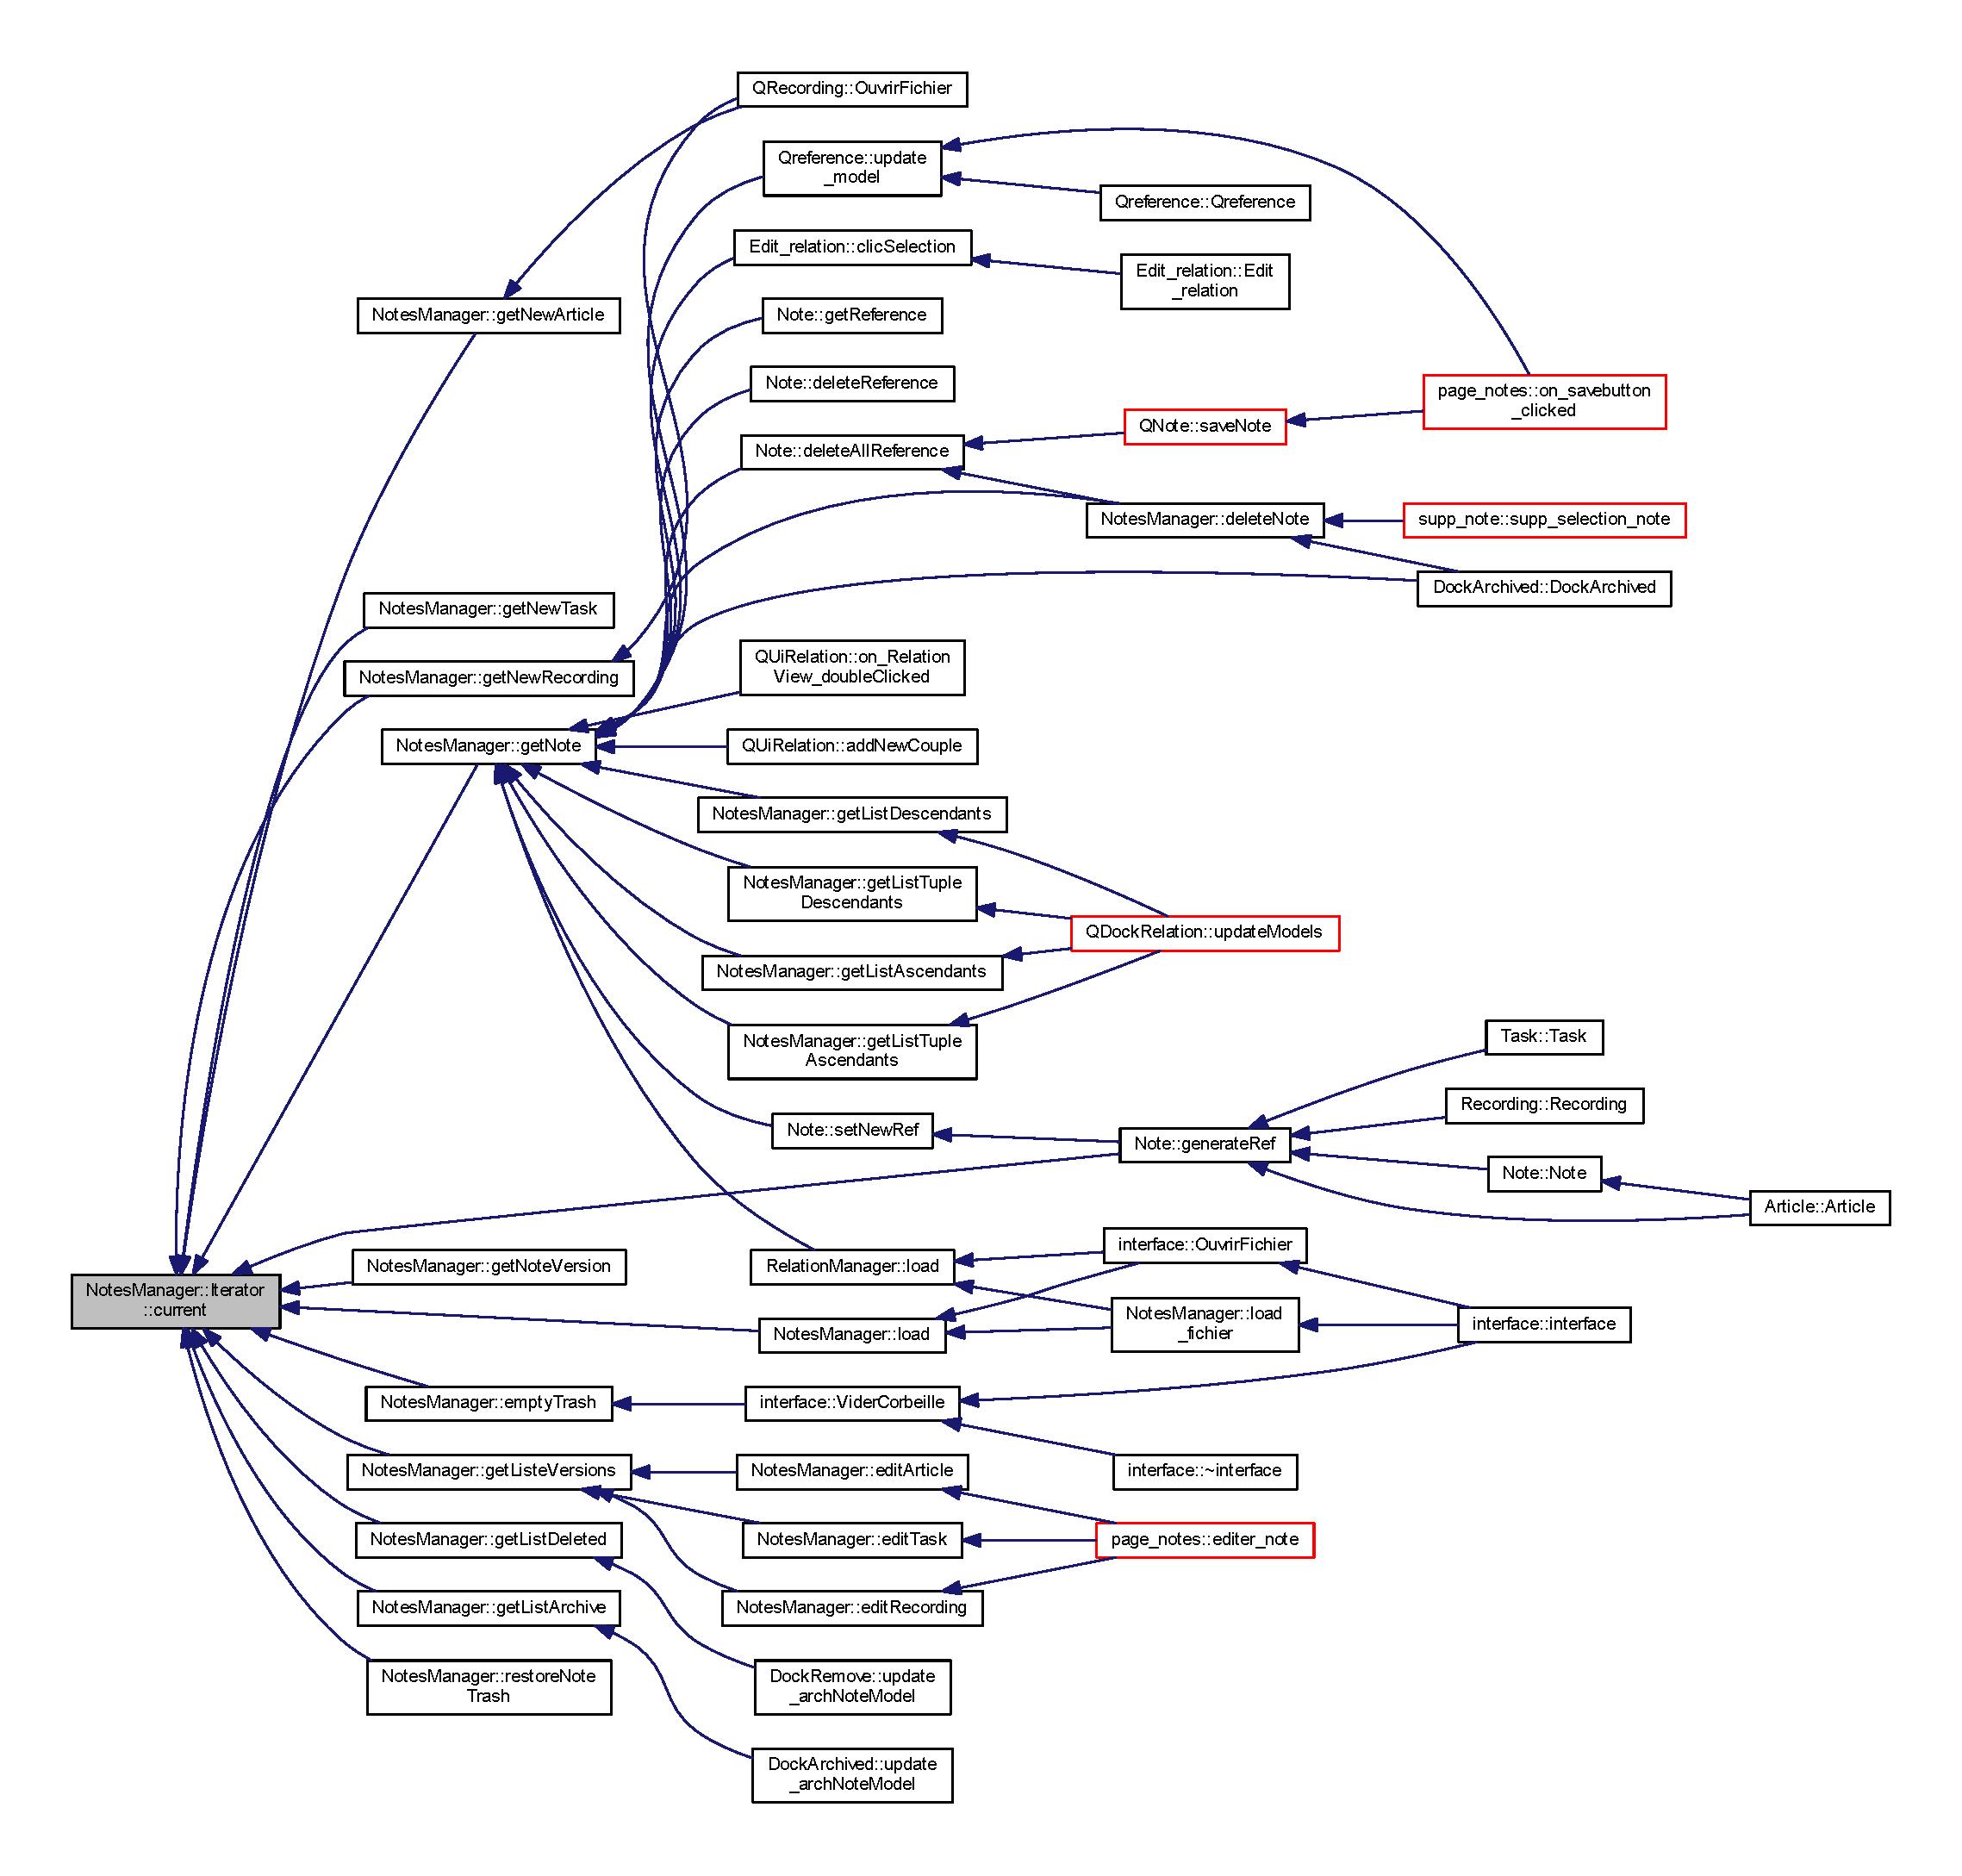
\includegraphics[width=350pt]{class_notes_manager_1_1_iterator_a4fd73444f2edd5f196d7b950527f5a90_icgraph}
\end{center}
\end{figure}
\mbox{\Hypertarget{class_notes_manager_1_1_iterator_a09a650ca2eeca614a4129ed5e1795e96}\label{class_notes_manager_1_1_iterator_a09a650ca2eeca614a4129ed5e1795e96}} 
\index{Notes\+Manager\+::\+Iterator@{Notes\+Manager\+::\+Iterator}!get\+Iterator\+Versions@{get\+Iterator\+Versions}}
\index{get\+Iterator\+Versions@{get\+Iterator\+Versions}!Notes\+Manager\+::\+Iterator@{Notes\+Manager\+::\+Iterator}}
\subsubsection{\texorpdfstring{get\+Iterator\+Versions()}{getIteratorVersions()}}
{\footnotesize\ttfamily Notes\+Manager\+::\+Iterator\+::get\+Iterator\+Versions (\begin{DoxyParamCaption}{ }\end{DoxyParamCaption})\hspace{0.3cm}{\ttfamily [inline]}}



Renvoie un itérateur sur les versions de la note courante. 

\begin{DoxyReturn}{Returns}
Q\+List$<$\+Note$\ast$$>$\+::iterator 
\end{DoxyReturn}


Definition at line 187 of file manager.\+h.

\mbox{\Hypertarget{class_notes_manager_1_1_iterator_a09b30631af5b7627b2b5a655a8ac450d}\label{class_notes_manager_1_1_iterator_a09b30631af5b7627b2b5a655a8ac450d}} 
\index{Notes\+Manager\+::\+Iterator@{Notes\+Manager\+::\+Iterator}!is\+Done@{is\+Done}}
\index{is\+Done@{is\+Done}!Notes\+Manager\+::\+Iterator@{Notes\+Manager\+::\+Iterator}}
\subsubsection{\texorpdfstring{is\+Done()}{isDone()}}
{\footnotesize\ttfamily Notes\+Manager\+::\+Iterator\+::is\+Done (\begin{DoxyParamCaption}{ }\end{DoxyParamCaption}) const\hspace{0.3cm}{\ttfamily [inline]}}



Vérifie si l\textquotesingle{}itérateur est arrivé à la fin de la liste. 

\begin{DoxyReturn}{Returns}
bool 
\end{DoxyReturn}


Definition at line 169 of file manager.\+h.

Here is the caller graph for this function\+:
\nopagebreak
\begin{figure}[H]
\begin{center}
\leavevmode
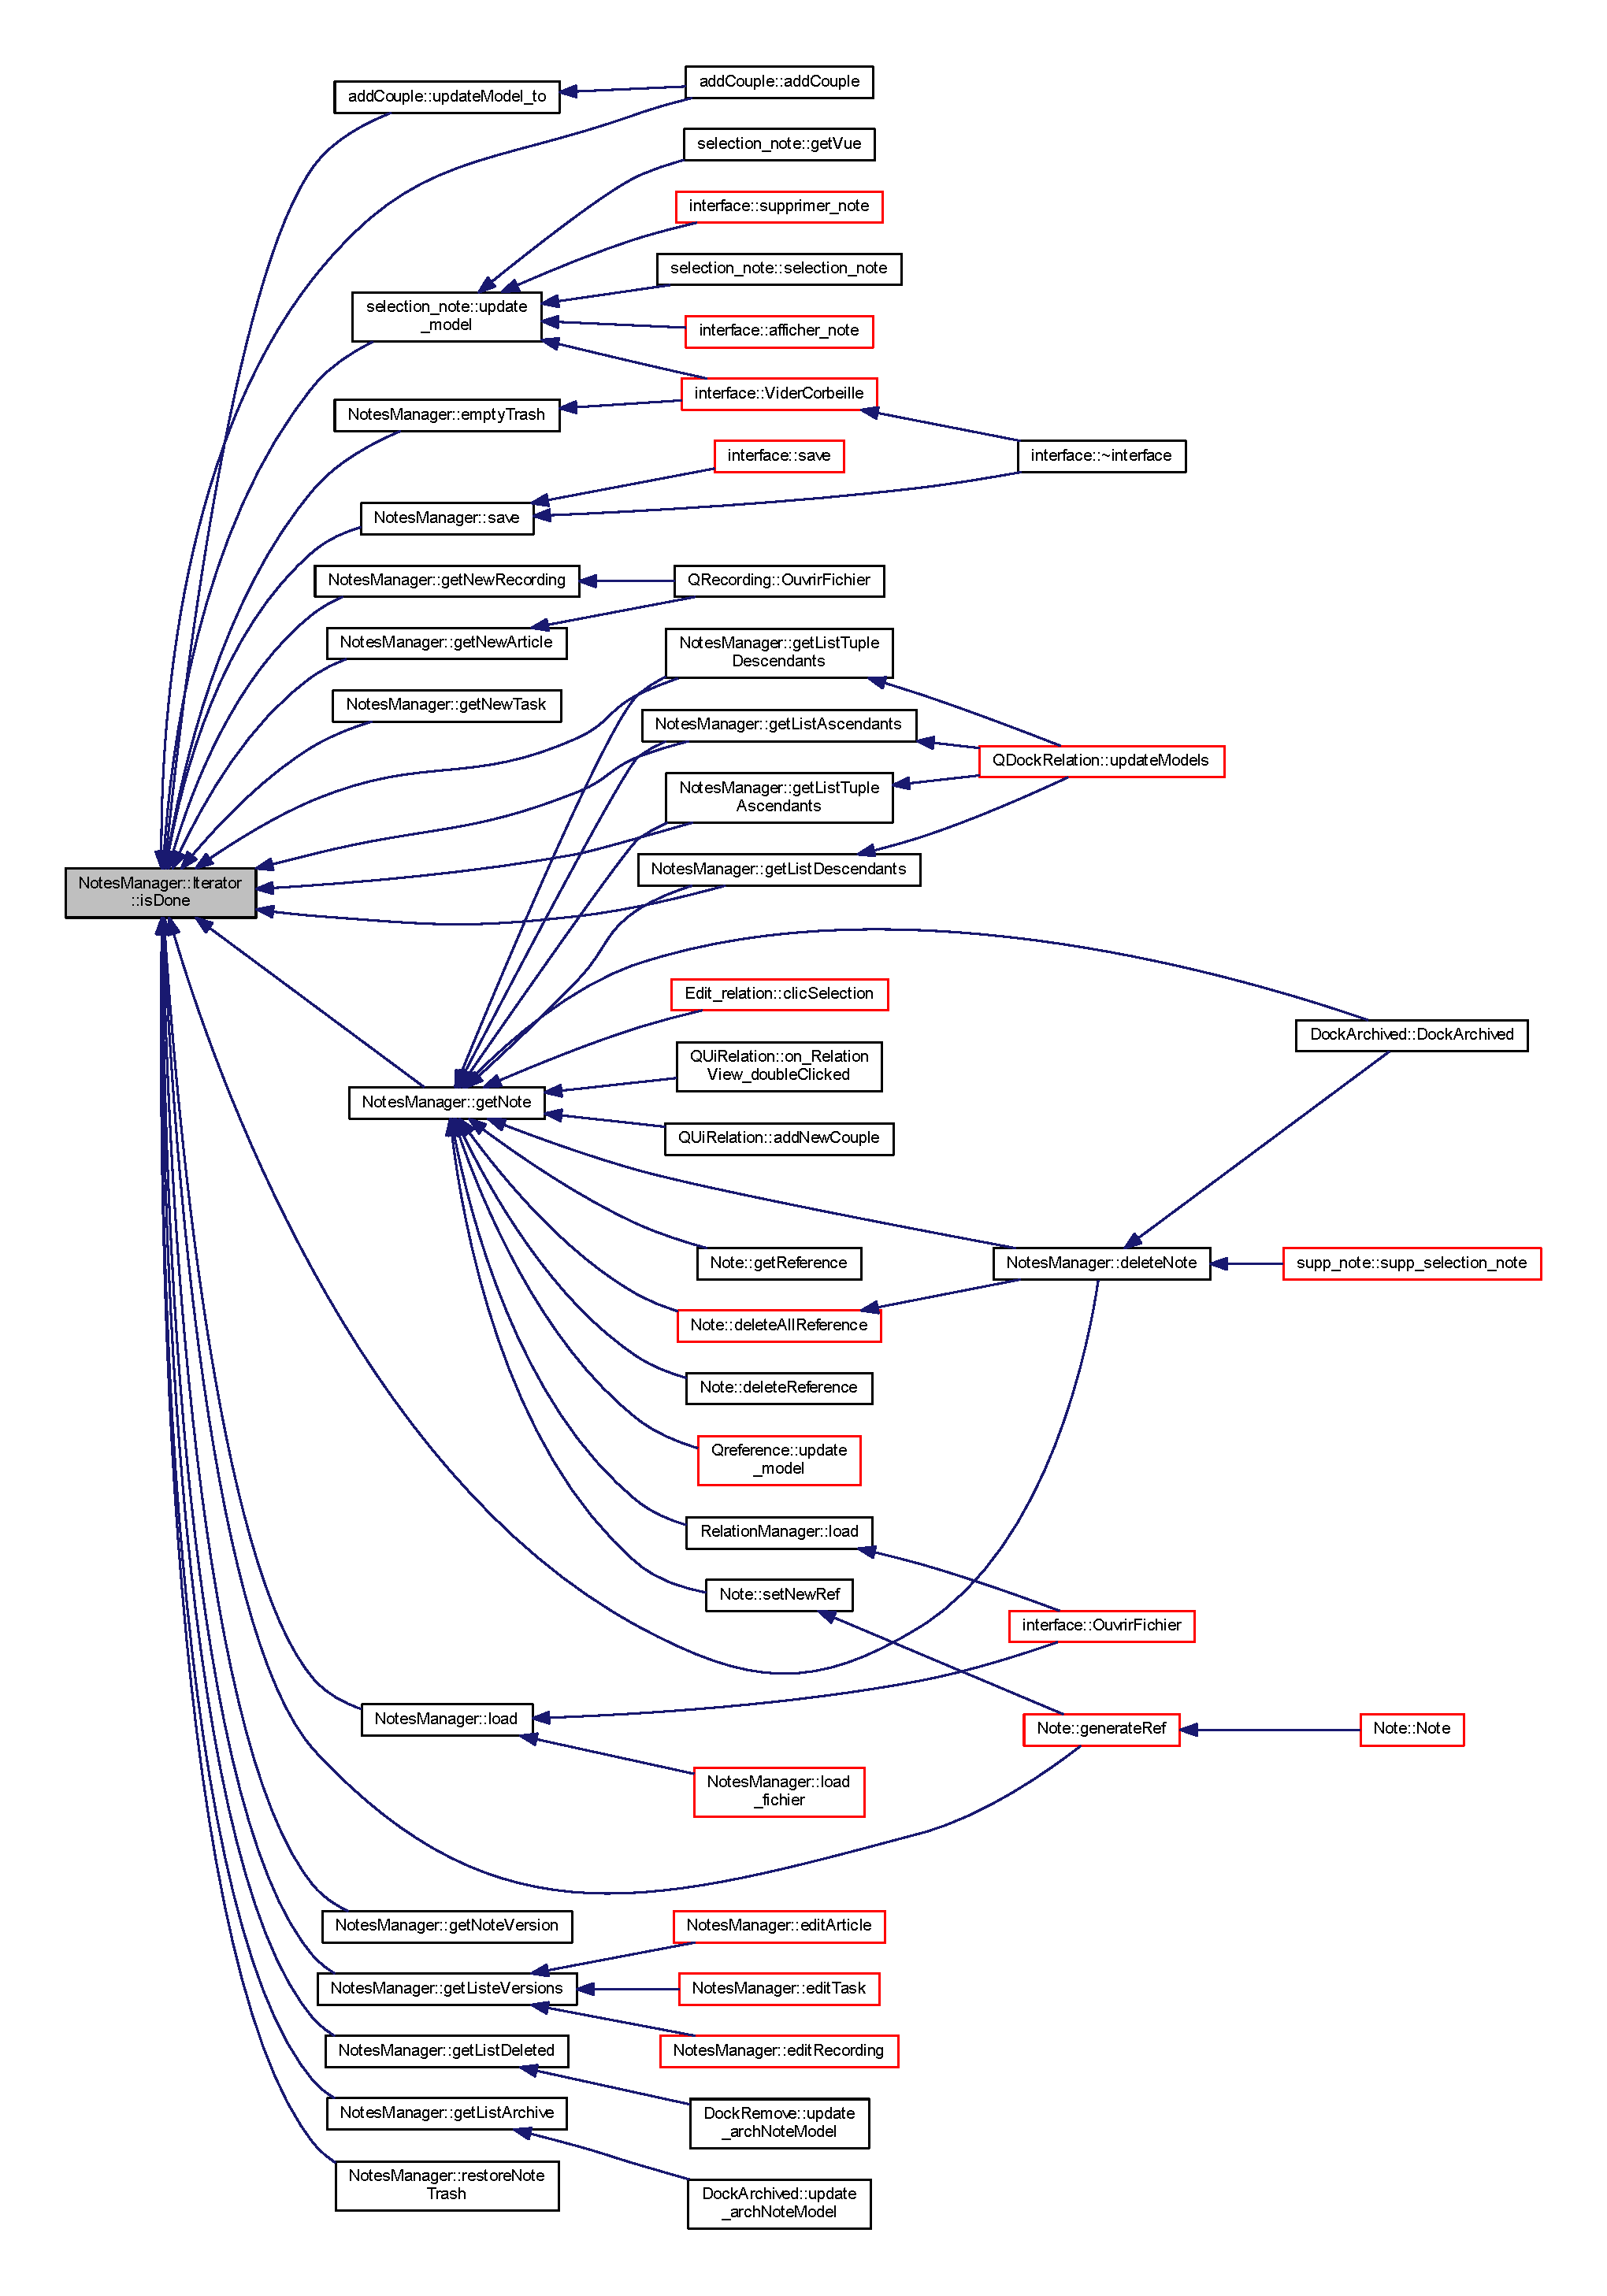
\includegraphics[width=350pt]{class_notes_manager_1_1_iterator_a09b30631af5b7627b2b5a655a8ac450d_icgraph}
\end{center}
\end{figure}
\mbox{\Hypertarget{class_notes_manager_1_1_iterator_a99e3eb098c3b5c7b3041731d10a18c88}\label{class_notes_manager_1_1_iterator_a99e3eb098c3b5c7b3041731d10a18c88}} 
\index{Notes\+Manager\+::\+Iterator@{Notes\+Manager\+::\+Iterator}!liste@{liste}}
\index{liste@{liste}!Notes\+Manager\+::\+Iterator@{Notes\+Manager\+::\+Iterator}}
\subsubsection{\texorpdfstring{liste()}{liste()}}
{\footnotesize\ttfamily Notes\+Manager\+::\+Iterator\+::liste (\begin{DoxyParamCaption}{ }\end{DoxyParamCaption})\hspace{0.3cm}{\ttfamily [inline]}}



Retourne la liste des toutes les versions de la note courante. 

\begin{DoxyReturn}{Returns}
Q\+List$<$\+Note$\ast$$>$$\ast$$\ast$ 
\end{DoxyReturn}


Definition at line 181 of file manager.\+h.

Here is the caller graph for this function\+:
\nopagebreak
\begin{figure}[H]
\begin{center}
\leavevmode
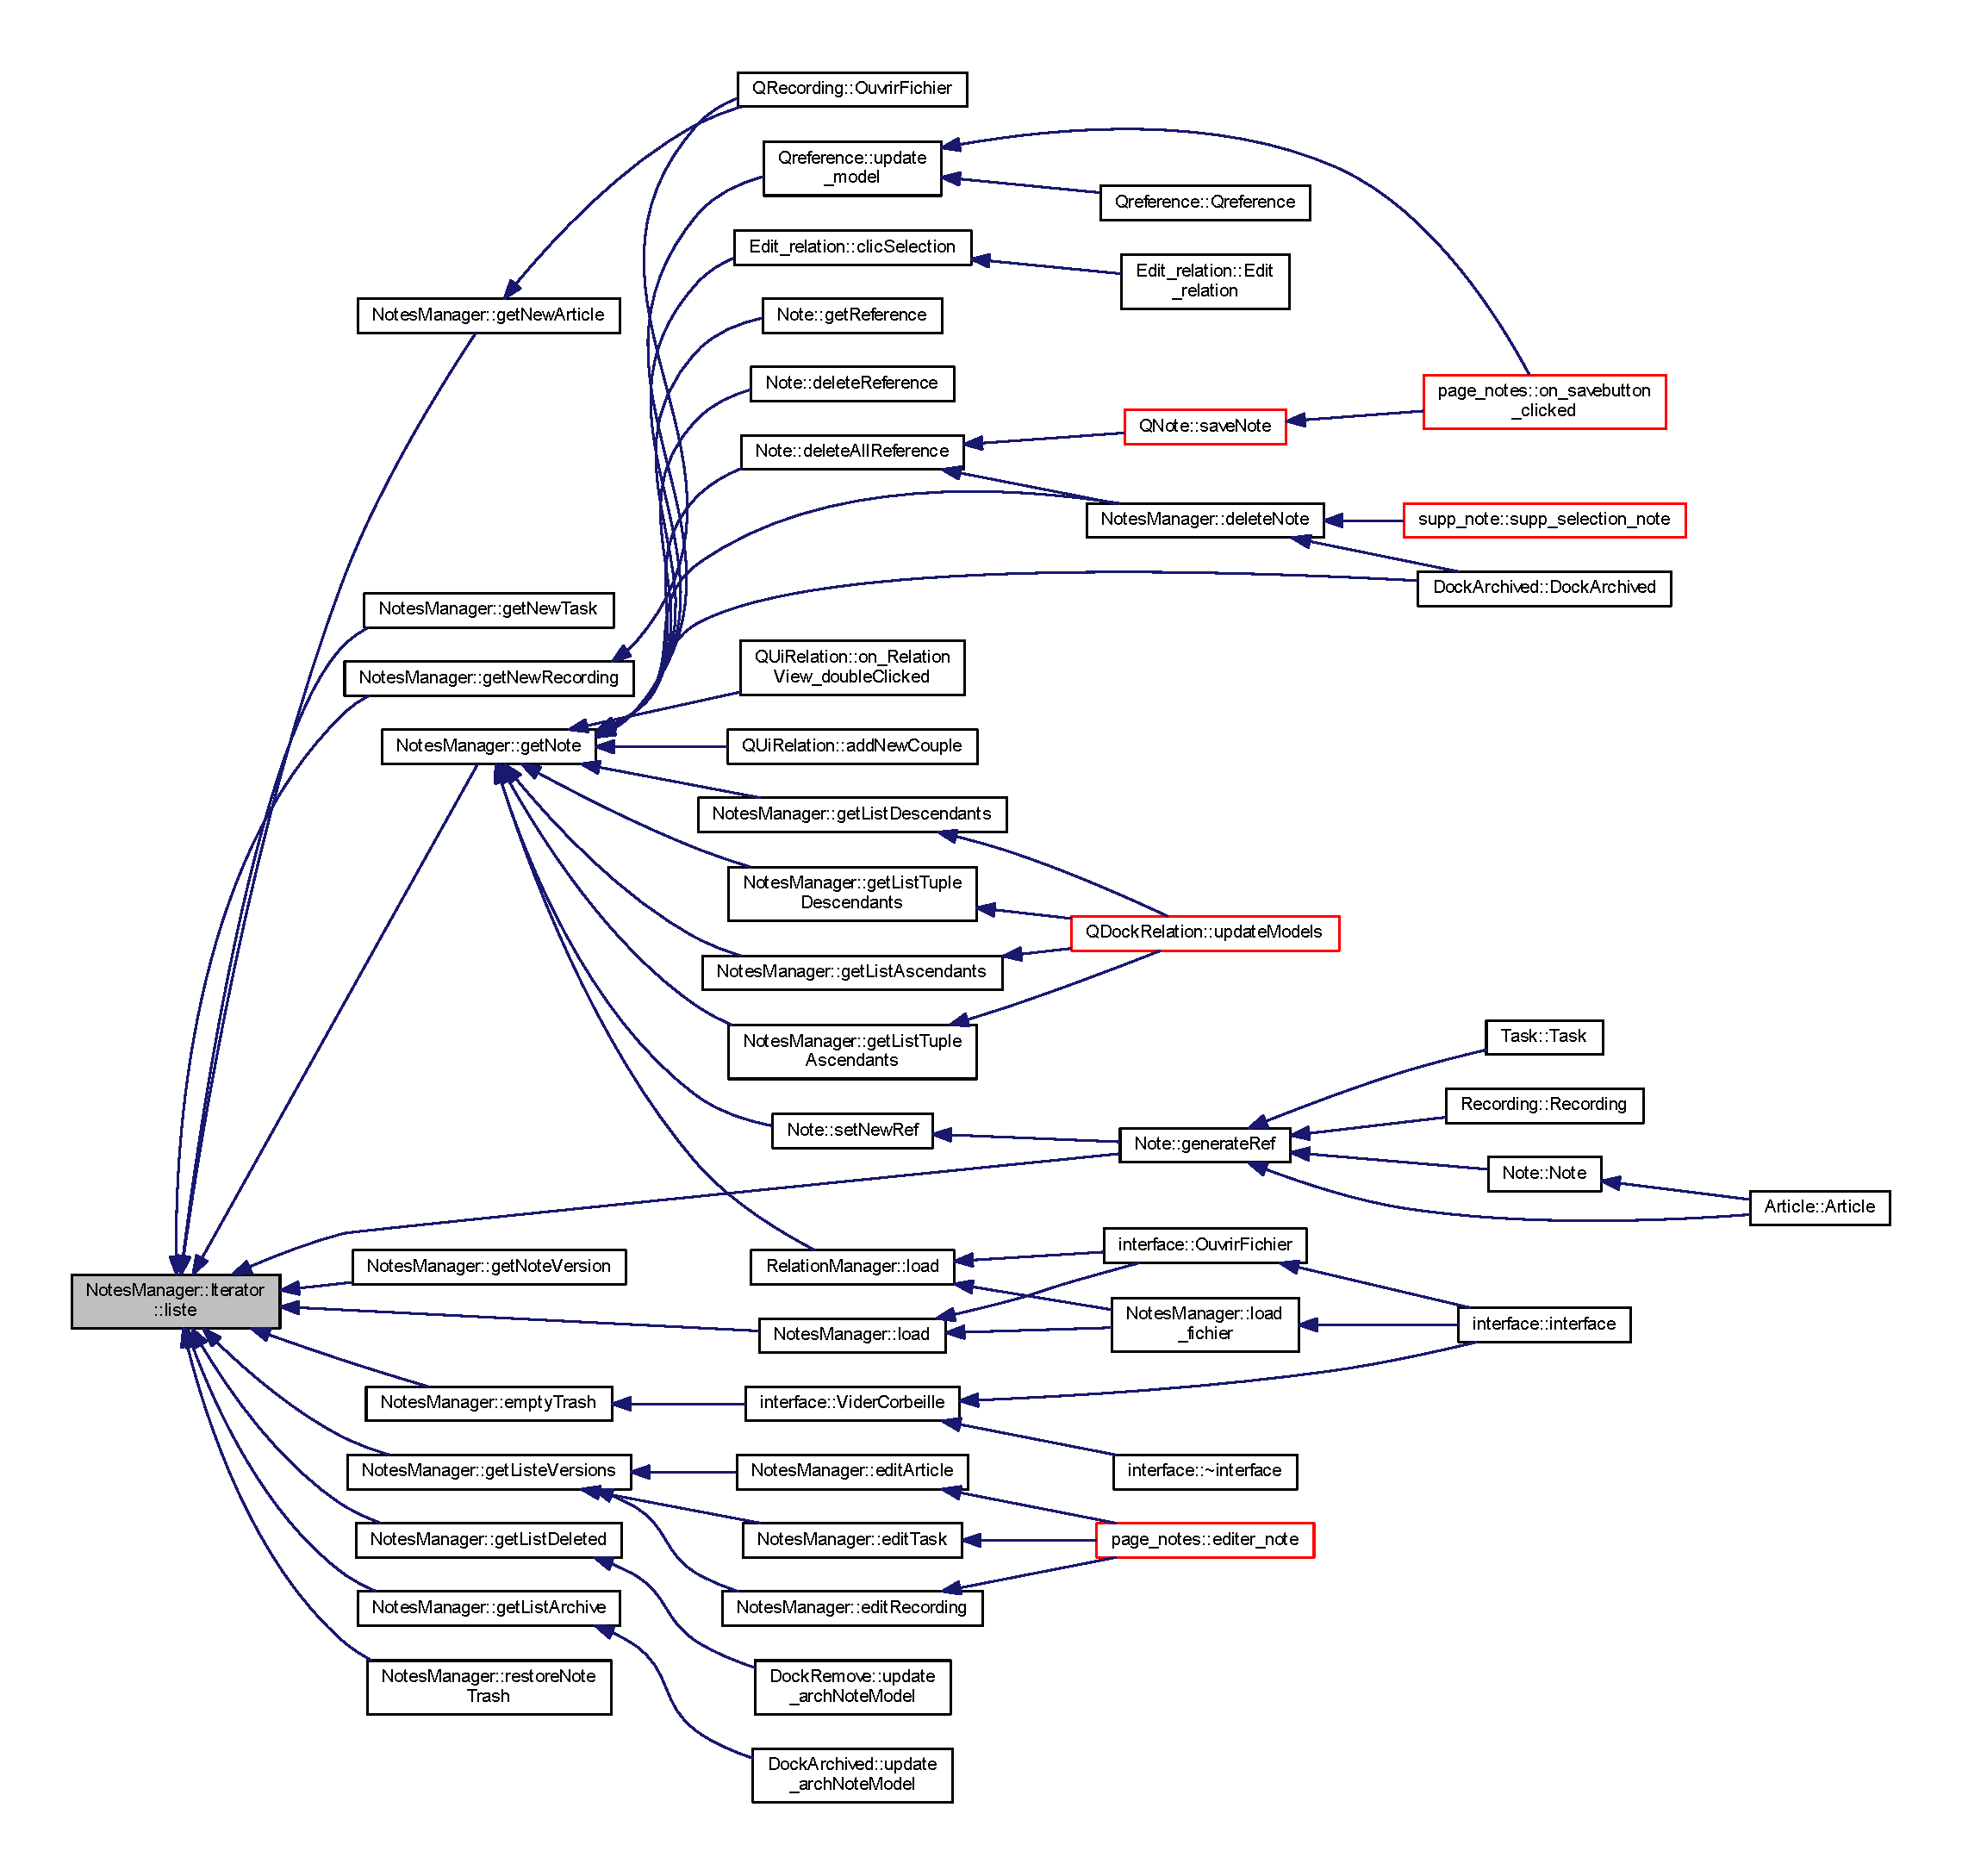
\includegraphics[width=350pt]{class_notes_manager_1_1_iterator_a99e3eb098c3b5c7b3041731d10a18c88_icgraph}
\end{center}
\end{figure}


The documentation for this class was generated from the following file\+:\begin{DoxyCompactItemize}
\item 
O\+L13/\hyperlink{manager_8h}{manager.\+h}\end{DoxyCompactItemize}

\hypertarget{class_note}{}\section{Note Class Reference}
\label{class_note}\index{Note@{Note}}


Inheritance diagram for Note\+:\nopagebreak
\begin{figure}[H]
\begin{center}
\leavevmode
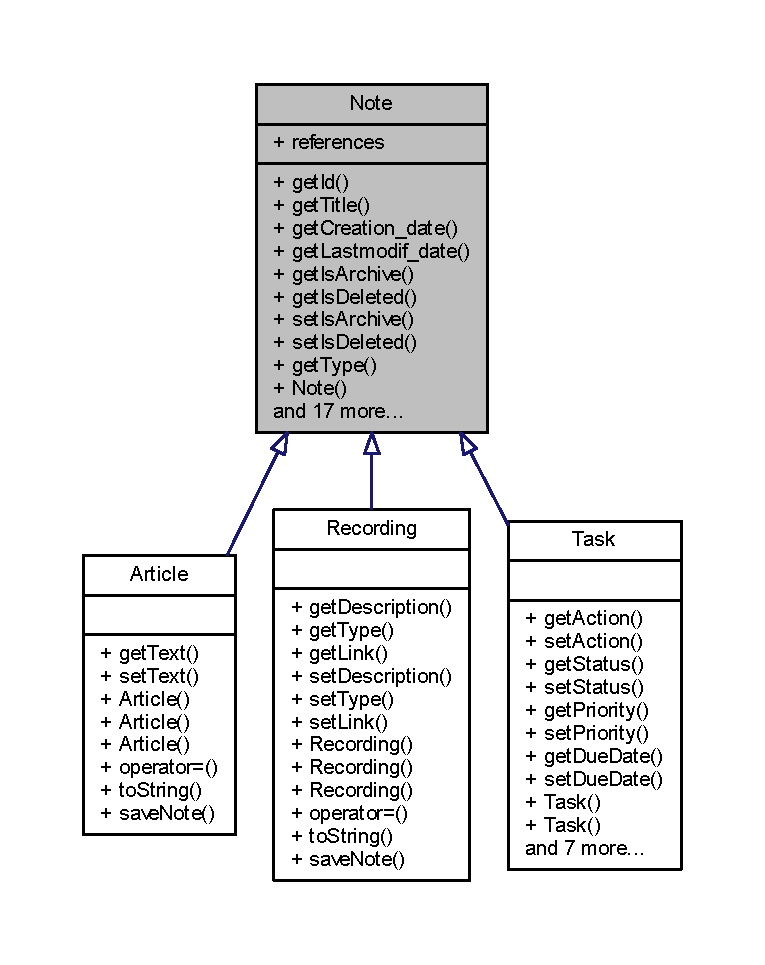
\includegraphics[width=350pt]{class_note__inherit__graph}
\end{center}
\end{figure}


Collaboration diagram for Note\+:\nopagebreak
\begin{figure}[H]
\begin{center}
\leavevmode
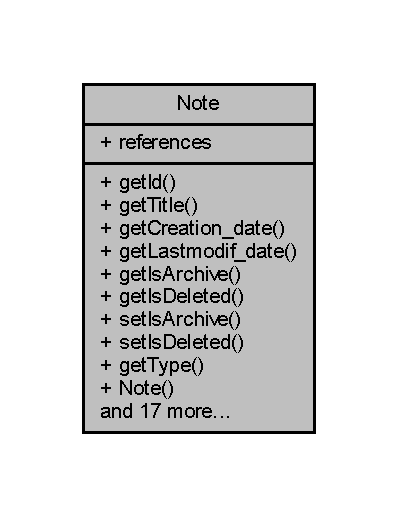
\includegraphics[width=191pt]{class_note__coll__graph}
\end{center}
\end{figure}
\subsection*{Public Member Functions}
\begin{DoxyCompactItemize}
\item 
\mbox{\Hypertarget{class_note_a8a7271e7e9f3fcc04944361f7ea0b846}\label{class_note_a8a7271e7e9f3fcc04944361f7ea0b846}} 
const Q\+String {\bfseries get\+Id} () const
\item 
\mbox{\Hypertarget{class_note_a7cd1137ae025c9495c5c24b1db90cbb3}\label{class_note_a7cd1137ae025c9495c5c24b1db90cbb3}} 
const Q\+String {\bfseries get\+Title} () const
\item 
\mbox{\Hypertarget{class_note_af29efb383791ec5d16f6db3fb5c7205d}\label{class_note_af29efb383791ec5d16f6db3fb5c7205d}} 
const Q\+Date\+Time {\bfseries get\+Creation\+\_\+date} () const
\item 
\mbox{\Hypertarget{class_note_a394327fab9f02f4d4e87b3ee78d99121}\label{class_note_a394327fab9f02f4d4e87b3ee78d99121}} 
const Q\+Date\+Time {\bfseries get\+Lastmodif\+\_\+date} () const
\item 
\mbox{\Hypertarget{class_note_a8fc3517be2c98114e1912080b7f12d57}\label{class_note_a8fc3517be2c98114e1912080b7f12d57}} 
bool {\bfseries get\+Is\+Archive} () const
\item 
\mbox{\Hypertarget{class_note_a76e4262b2c064b8ec4791ab1316d5568}\label{class_note_a76e4262b2c064b8ec4791ab1316d5568}} 
bool {\bfseries get\+Is\+Deleted} () const
\item 
\mbox{\Hypertarget{class_note_a4174e5bcefa138c9e5d55b34239b2e5d}\label{class_note_a4174e5bcefa138c9e5d55b34239b2e5d}} 
void {\bfseries set\+Is\+Archive} (bool a)
\item 
\mbox{\Hypertarget{class_note_ae112c975e37801222608656927568a37}\label{class_note_ae112c975e37801222608656927568a37}} 
void {\bfseries set\+Is\+Deleted} (bool d)
\item 
\mbox{\Hypertarget{class_note_ad6325df1dc1410d7854cac36ff312b8c}\label{class_note_ad6325df1dc1410d7854cac36ff312b8c}} 
Q\+String {\bfseries get\+Type} () const
\item 
\hyperlink{class_note_a0490153115307d5f59974d7000260e48}{Note} (const Q\+String \&i, const Q\+String \&ti)
\begin{DoxyCompactList}\small\item\em Constructeur des classes notes, articles task et recording. \end{DoxyCompactList}\item 
\mbox{\Hypertarget{class_note_a0c1c2ba85358585f266b0fdcbcb45a70}\label{class_note_a0c1c2ba85358585f266b0fdcbcb45a70}} 
{\bfseries Note} (const Q\+String \&i, const Q\+String \&ti, const Q\+Date\+Time \&cd, const Q\+Date\+Time \&lmd, bool iA, bool iD)
\item 
\mbox{\Hypertarget{class_note_a7a9ca310664f058b56ccc33005688e25}\label{class_note_a7a9ca310664f058b56ccc33005688e25}} 
void {\bfseries set\+Title} (const Q\+String \&t)
\item 
\mbox{\Hypertarget{class_note_ab83acc1404775a43af17a31edeaae246}\label{class_note_ab83acc1404775a43af17a31edeaae246}} 
void {\bfseries set\+Creation\+\_\+date} (const Q\+Date\+Time \&d)
\item 
\mbox{\Hypertarget{class_note_a2cb5616e643b49316bd95e9a2b958e44}\label{class_note_a2cb5616e643b49316bd95e9a2b958e44}} 
void {\bfseries set\+Lastmodif\+\_\+date} (const Q\+Date\+Time \&d)
\item 
\hyperlink{class_note_ac06fd282c05bbfe2e1675fe0677b2efb}{Note} (const \hyperlink{class_note}{Note} \&n)
\begin{DoxyCompactList}\small\item\em Constructeur de recopie. \end{DoxyCompactList}\item 
\mbox{\Hypertarget{class_note_ac9b2b6b880bd4c01738ee43bde04b7e5}\label{class_note_ac9b2b6b880bd4c01738ee43bde04b7e5}} 
\hyperlink{class_note}{Note} \& \hyperlink{class_note_ac9b2b6b880bd4c01738ee43bde04b7e5}{operator=} (const \hyperlink{class_note}{Note} \&n)
\begin{DoxyCompactList}\small\item\em Surcharge de l\textquotesingle{}opérateur = dans le cas nouvelle note B=A. \end{DoxyCompactList}\item 
\mbox{\Hypertarget{class_note_ade484273015c82e7fa59a028de0d8818}\label{class_note_ade484273015c82e7fa59a028de0d8818}} 
virtual \hyperlink{class_note_ade484273015c82e7fa59a028de0d8818}{$\sim$\+Note} ()
\begin{DoxyCompactList}\small\item\em Destructeur de la classe \hyperlink{class_note}{Note}. \end{DoxyCompactList}\item 
virtual std\+::string \hyperlink{class_note_a1bd4acfbde0b71d05fd7d4ca889bca2b}{to\+String} () const
\begin{DoxyCompactList}\small\item\em Transforme une note en un flux ostream a afficher. \end{DoxyCompactList}\item 
\mbox{\Hypertarget{class_note_a00684fea94bcdcf16f9d40a9d7a8dd5b}\label{class_note_a00684fea94bcdcf16f9d40a9d7a8dd5b}} 
void {\bfseries display} (std\+::ostream \&f=std\+::cout) const
\item 
\mbox{\Hypertarget{class_note_a0c2cc72d7f3235c665a30ef915c5c58d}\label{class_note_a0c2cc72d7f3235c665a30ef915c5c58d}} 
virtual void {\bfseries save\+Note} (Q\+File $\ast$file)
\item 
\mbox{\Hypertarget{class_note_acf0ffc4f88903851dce3abf75c3d53f2}\label{class_note_acf0ffc4f88903851dce3abf75c3d53f2}} 
void {\bfseries set\+Nb\+Is\+Ref} (unsigned int n)
\item 
\mbox{\Hypertarget{class_note_a1cb41601ca2dc7c020053c4c0b58f12e}\label{class_note_a1cb41601ca2dc7c020053c4c0b58f12e}} 
unsigned int {\bfseries get\+Nb\+Is\+Ref} () const
\item 
void \hyperlink{class_note_a91c86cf6ed18e4badb59a41e737a15fa}{delete\+Reference} (const Q\+String \&id)
\begin{DoxyCompactList}\small\item\em Supprime la référence sur une note spécifiée par son ID. \end{DoxyCompactList}\item 
void \hyperlink{class_note_aacbb89b120107a4b25dd16043908c693}{delete\+All\+Reference} ()
\begin{DoxyCompactList}\small\item\em Supprime l\textquotesingle{}ensemble des références d\textquotesingle{}une note. \end{DoxyCompactList}\item 
void \hyperlink{class_note_a3af2edc369310b9f122bd1fd6dbfa717}{set\+New\+Ref} (const Q\+String \&id)
\begin{DoxyCompactList}\small\item\em Définie une note comme référence d\textquotesingle{}une autre. \end{DoxyCompactList}\item 
\hyperlink{class_note}{Note} \& \hyperlink{class_note_a8e3ba6961f62a38f49b5fd209c083896}{get\+Reference} (const Q\+String \&id) const
\begin{DoxyCompactList}\small\item\em Retourne une note référencée par une autre. \end{DoxyCompactList}\item 
void \hyperlink{class_note_a5a0cb370ddd5a3da10fe8aa8a256d661}{generate\+Ref} (const Q\+String \&champ\+Texte)
\begin{DoxyCompactList}\small\item\em Détecte la présence d\textquotesingle{}une expression régulière dans un champ de text et ajoute une référence en conséquence. \end{DoxyCompactList}\end{DoxyCompactItemize}
\subsection*{Public Attributes}
\begin{DoxyCompactItemize}
\item 
\mbox{\Hypertarget{class_note_ad8918cd74c86c9e00d72cb1a6a5a0f88}\label{class_note_ad8918cd74c86c9e00d72cb1a6a5a0f88}} 
Q\+List$<$ Q\+String $>$ {\bfseries references}
\end{DoxyCompactItemize}


\subsection{Detailed Description}


Definition at line 74 of file notes.\+h.



\subsection{Constructor \& Destructor Documentation}
\mbox{\Hypertarget{class_note_a0490153115307d5f59974d7000260e48}\label{class_note_a0490153115307d5f59974d7000260e48}} 
\index{Note@{Note}!Note@{Note}}
\index{Note@{Note}!Note@{Note}}
\subsubsection{\texorpdfstring{Note()}{Note()}\hspace{0.1cm}{\footnotesize\ttfamily [1/2]}}
{\footnotesize\ttfamily Note\+::\+Note (\begin{DoxyParamCaption}\item[{const Q\+String \&}]{i,  }\item[{const Q\+String \&}]{ti }\end{DoxyParamCaption})}



Constructeur des classes notes, articles task et recording. 

Les classes dérivées \hyperlink{class_article}{Article}, \hyperlink{class_task}{Task}, \hyperlink{class_recording}{Recording} utilise en premier lieu le constructeur de \hyperlink{class_note}{Note}. Dans le constructeur de \hyperlink{class_note}{Note}, la date de création et de dernière modification sont mises à jours avec la date courrante. 

Definition at line 106 of file notes.\+cpp.

Here is the call graph for this function\+:\nopagebreak
\begin{figure}[H]
\begin{center}
\leavevmode
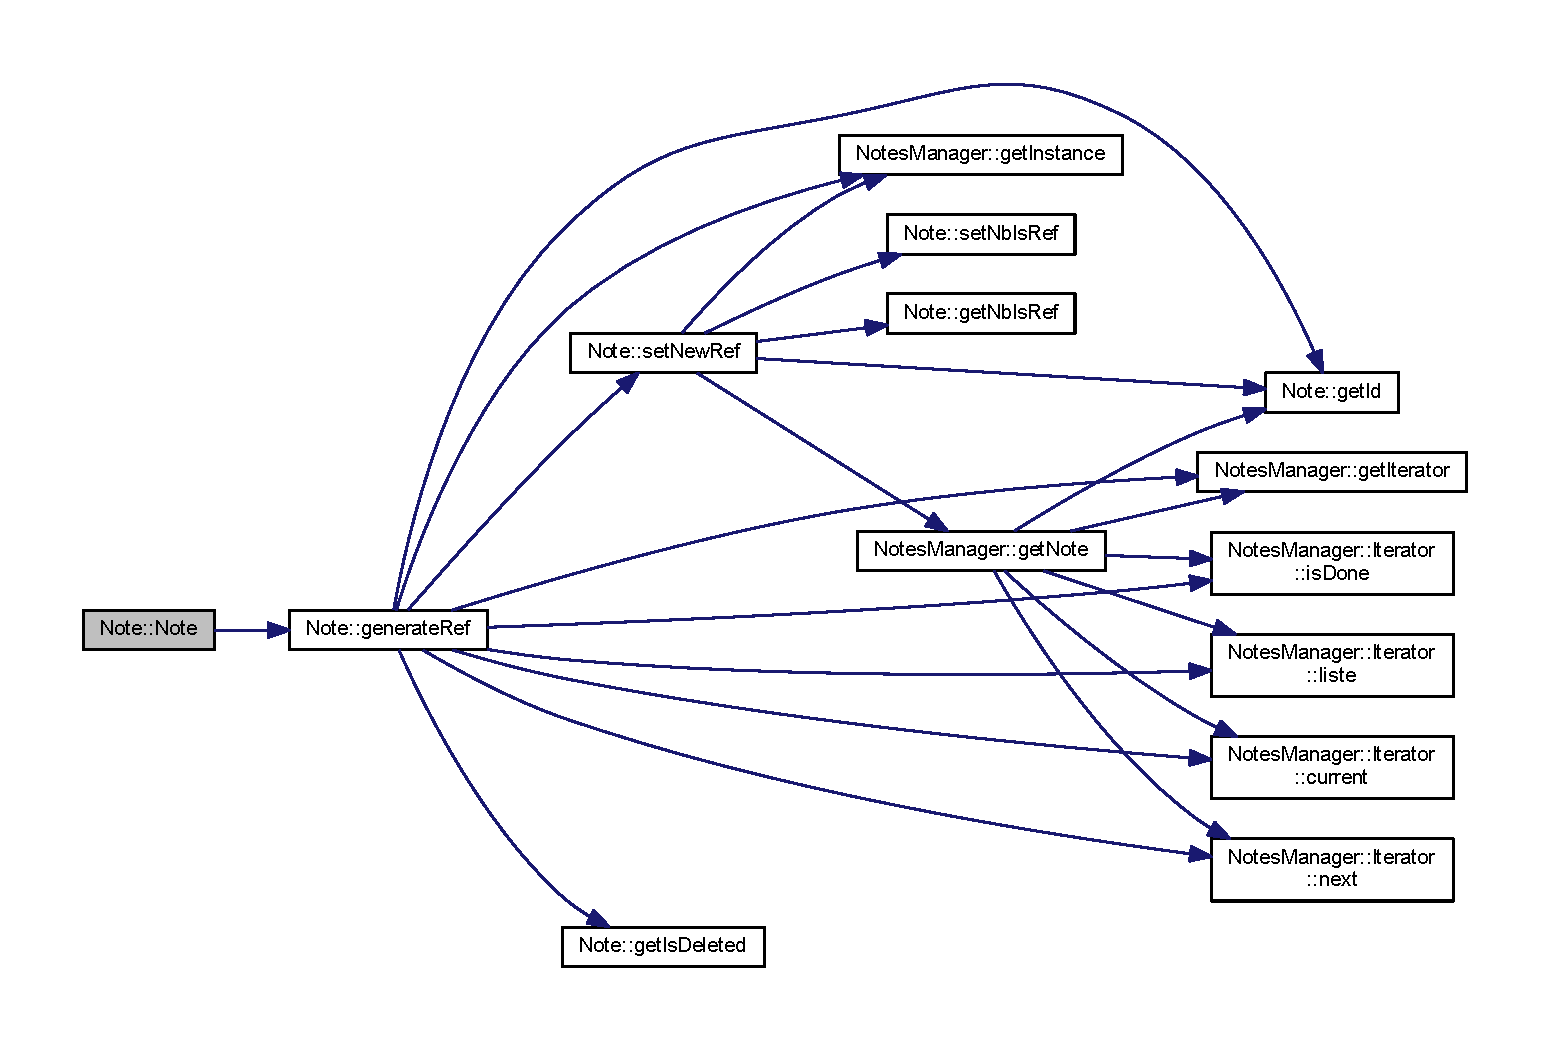
\includegraphics[width=350pt]{class_note_a0490153115307d5f59974d7000260e48_cgraph}
\end{center}
\end{figure}
Here is the caller graph for this function\+:\nopagebreak
\begin{figure}[H]
\begin{center}
\leavevmode
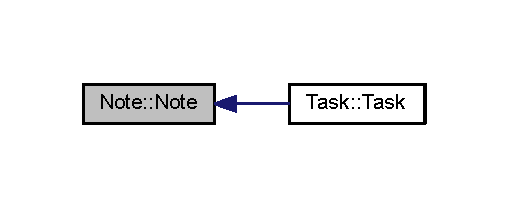
\includegraphics[width=244pt]{class_note_a0490153115307d5f59974d7000260e48_icgraph}
\end{center}
\end{figure}
\mbox{\Hypertarget{class_note_ac06fd282c05bbfe2e1675fe0677b2efb}\label{class_note_ac06fd282c05bbfe2e1675fe0677b2efb}} 
\index{Note@{Note}!Note@{Note}}
\index{Note@{Note}!Note@{Note}}
\subsubsection{\texorpdfstring{Note()}{Note()}\hspace{0.1cm}{\footnotesize\ttfamily [2/2]}}
{\footnotesize\ttfamily Note\+::\+Note (\begin{DoxyParamCaption}\item[{const \hyperlink{class_note}{Note} \&}]{n }\end{DoxyParamCaption})}



Constructeur de recopie. 

Recopie l\textquotesingle{}ensemble des informations d\textquotesingle{}une note Mets à jour la date de dernière modification avec current\+Date\+Time. 
\begin{DoxyParams}{Parameters}
{\em const} & \hyperlink{class_note}{Note}\& n La note a recopier. \\
\hline
\end{DoxyParams}


Definition at line 35 of file notes.\+cpp.



\subsection{Member Function Documentation}
\mbox{\Hypertarget{class_note_aacbb89b120107a4b25dd16043908c693}\label{class_note_aacbb89b120107a4b25dd16043908c693}} 
\index{Note@{Note}!delete\+All\+Reference@{delete\+All\+Reference}}
\index{delete\+All\+Reference@{delete\+All\+Reference}!Note@{Note}}
\subsubsection{\texorpdfstring{delete\+All\+Reference()}{deleteAllReference()}}
{\footnotesize\ttfamily void Note\+::delete\+All\+Reference (\begin{DoxyParamCaption}{ }\end{DoxyParamCaption})}



Supprime l\textquotesingle{}ensemble des références d\textquotesingle{}une note. 

À chaque suppression, les notes anciennement référencées par cette note diminuent le nombre de notes qui les référence. 

Definition at line 399 of file notes.\+cpp.

Here is the call graph for this function\+:\nopagebreak
\begin{figure}[H]
\begin{center}
\leavevmode
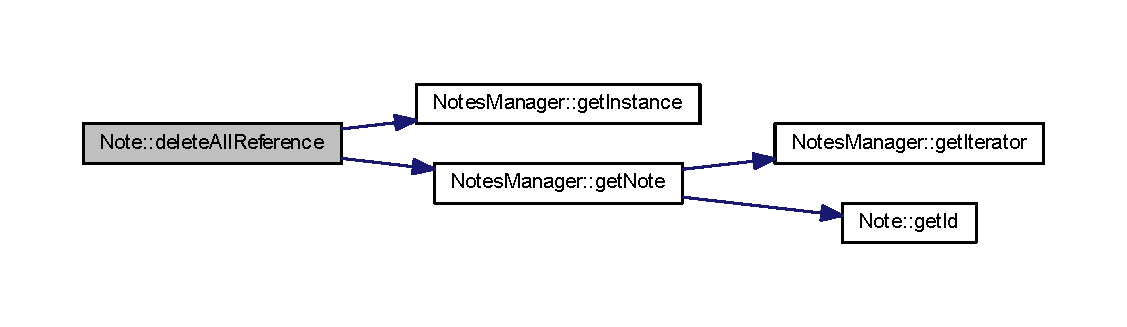
\includegraphics[width=350pt]{class_note_aacbb89b120107a4b25dd16043908c693_cgraph}
\end{center}
\end{figure}
Here is the caller graph for this function\+:\nopagebreak
\begin{figure}[H]
\begin{center}
\leavevmode
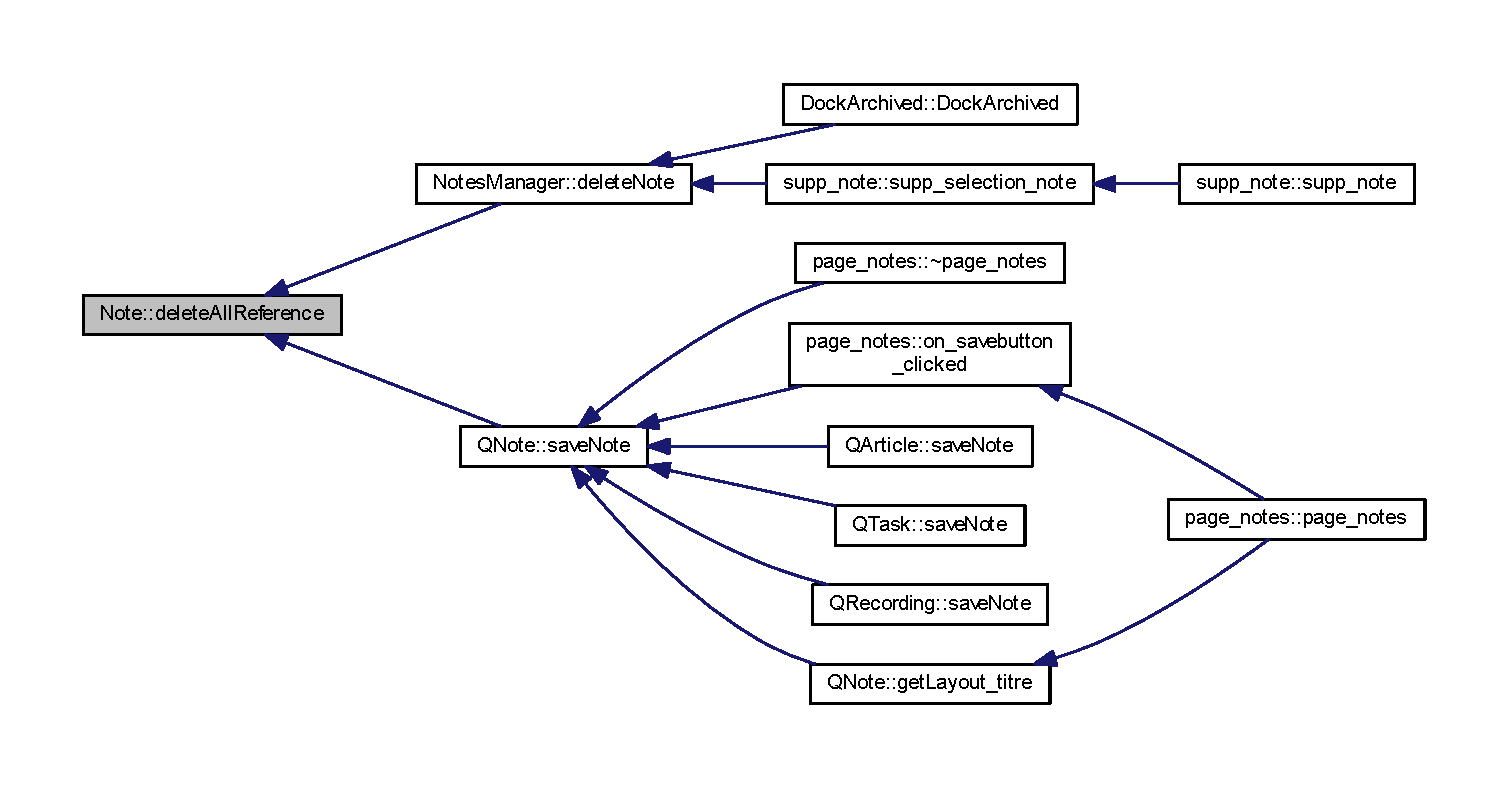
\includegraphics[width=350pt]{class_note_aacbb89b120107a4b25dd16043908c693_icgraph}
\end{center}
\end{figure}
\mbox{\Hypertarget{class_note_a91c86cf6ed18e4badb59a41e737a15fa}\label{class_note_a91c86cf6ed18e4badb59a41e737a15fa}} 
\index{Note@{Note}!delete\+Reference@{delete\+Reference}}
\index{delete\+Reference@{delete\+Reference}!Note@{Note}}
\subsubsection{\texorpdfstring{delete\+Reference()}{deleteReference()}}
{\footnotesize\ttfamily void Note\+::delete\+Reference (\begin{DoxyParamCaption}\item[{const Q\+String \&}]{id }\end{DoxyParamCaption})}



Supprime la référence sur une note spécifiée par son ID. 


\begin{DoxyParams}{Parameters}
{\em const} & Q\+String\& id L\textquotesingle{}ID de la note référencée a supprimer. \\
\hline
\end{DoxyParams}


Definition at line 374 of file notes.\+cpp.

Here is the call graph for this function\+:\nopagebreak
\begin{figure}[H]
\begin{center}
\leavevmode
\includegraphics[width=350pt]{class_note_a91c86cf6ed18e4badb59a41e737a15fa_cgraph}
\end{center}
\end{figure}
\mbox{\Hypertarget{class_note_a5a0cb370ddd5a3da10fe8aa8a256d661}\label{class_note_a5a0cb370ddd5a3da10fe8aa8a256d661}} 
\index{Note@{Note}!generate\+Ref@{generate\+Ref}}
\index{generate\+Ref@{generate\+Ref}!Note@{Note}}
\subsubsection{\texorpdfstring{generate\+Ref()}{generateRef()}}
{\footnotesize\ttfamily void Note\+::generate\+Ref (\begin{DoxyParamCaption}\item[{const Q\+String \&}]{champ\+Texte }\end{DoxyParamCaption})}



Détecte la présence d\textquotesingle{}une expression régulière dans un champ de text et ajoute une référence en conséquence. 

Cette méthode est appelée par le constructeur de notes et par les setters de champ de texte de notes. Si l\textquotesingle{}expression régulière \textbackslash{}\+:ref\{(.+)\} est repérée, et si l\textquotesingle{}ID retourné correspond à celui d\textquotesingle{}une note active, la note correspondant à l\textquotesingle{}ID est ajoutée en référence de la note this. 
\begin{DoxyParams}{Parameters}
{\em const} & Q\+String\& champ\+Texte champ de texte dans laquelle la regex doit être repérée \\
\hline
\end{DoxyParams}


Definition at line 418 of file notes.\+cpp.

Here is the call graph for this function\+:\nopagebreak
\begin{figure}[H]
\begin{center}
\leavevmode
\includegraphics[width=350pt]{class_note_a5a0cb370ddd5a3da10fe8aa8a256d661_cgraph}
\end{center}
\end{figure}
Here is the caller graph for this function\+:\nopagebreak
\begin{figure}[H]
\begin{center}
\leavevmode
\includegraphics[width=350pt]{class_note_a5a0cb370ddd5a3da10fe8aa8a256d661_icgraph}
\end{center}
\end{figure}
\mbox{\Hypertarget{class_note_a8e3ba6961f62a38f49b5fd209c083896}\label{class_note_a8e3ba6961f62a38f49b5fd209c083896}} 
\index{Note@{Note}!get\+Reference@{get\+Reference}}
\index{get\+Reference@{get\+Reference}!Note@{Note}}
\subsubsection{\texorpdfstring{get\+Reference()}{getReference()}}
{\footnotesize\ttfamily \hyperlink{class_note}{Note} \& Note\+::get\+Reference (\begin{DoxyParamCaption}\item[{const Q\+String \&}]{id }\end{DoxyParamCaption}) const}



Retourne une note référencée par une autre. 


\begin{DoxyParams}{Parameters}
{\em const} & Q\+String\& id L\textquotesingle{}ID de la note référencée. \\
\hline
\end{DoxyParams}


Definition at line 358 of file notes.\+cpp.

Here is the call graph for this function\+:\nopagebreak
\begin{figure}[H]
\begin{center}
\leavevmode
\includegraphics[width=350pt]{class_note_a8e3ba6961f62a38f49b5fd209c083896_cgraph}
\end{center}
\end{figure}
\mbox{\Hypertarget{class_note_a3af2edc369310b9f122bd1fd6dbfa717}\label{class_note_a3af2edc369310b9f122bd1fd6dbfa717}} 
\index{Note@{Note}!set\+New\+Ref@{set\+New\+Ref}}
\index{set\+New\+Ref@{set\+New\+Ref}!Note@{Note}}
\subsubsection{\texorpdfstring{set\+New\+Ref()}{setNewRef()}}
{\footnotesize\ttfamily void Note\+::set\+New\+Ref (\begin{DoxyParamCaption}\item[{const Q\+String \&}]{id }\end{DoxyParamCaption})}



Définie une note comme référence d\textquotesingle{}une autre. 

Lorsqu\textquotesingle{}une note prend comme référence une autre, cette autre note augmente son attribut nb\+Is\+Ref lui permettant de connaître le nombre de notes qui la référencent. 
\begin{DoxyParams}{Parameters}
{\em const} & Q\+String\& L\textquotesingle{}ID de la note référencée. \\
\hline
\end{DoxyParams}


Definition at line 344 of file notes.\+cpp.

Here is the call graph for this function\+:\nopagebreak
\begin{figure}[H]
\begin{center}
\leavevmode
\includegraphics[width=350pt]{class_note_a3af2edc369310b9f122bd1fd6dbfa717_cgraph}
\end{center}
\end{figure}
Here is the caller graph for this function\+:\nopagebreak
\begin{figure}[H]
\begin{center}
\leavevmode
\includegraphics[width=350pt]{class_note_a3af2edc369310b9f122bd1fd6dbfa717_icgraph}
\end{center}
\end{figure}
\mbox{\Hypertarget{class_note_a1bd4acfbde0b71d05fd7d4ca889bca2b}\label{class_note_a1bd4acfbde0b71d05fd7d4ca889bca2b}} 
\index{Note@{Note}!to\+String@{to\+String}}
\index{to\+String@{to\+String}!Note@{Note}}
\subsubsection{\texorpdfstring{to\+String()}{toString()}}
{\footnotesize\ttfamily std\+::string Note\+::to\+String (\begin{DoxyParamCaption}{ }\end{DoxyParamCaption}) const\hspace{0.3cm}{\ttfamily [virtual]}}



Transforme une note en un flux ostream a afficher. 

\begin{DoxyReturn}{Returns}
Le flux ostream 
\end{DoxyReturn}


Reimplemented in \hyperlink{class_recording_a9f403a39bec2db40c9171a6c3a20942d}{Recording}, \hyperlink{class_task_a7fe5cb7b57a21693e7abfea2f9618563}{Task}, and \hyperlink{class_article_ae40d268ecffbaaa549968a81ea609ba4}{Article}.



Definition at line 182 of file notes.\+cpp.



The documentation for this class was generated from the following files\+:\begin{DoxyCompactItemize}
\item 
O\+L13/notes.\+h\item 
O\+L13/\hyperlink{notes_8cpp}{notes.\+cpp}\end{DoxyCompactItemize}

\hypertarget{class_notes_couple}{}\section{Notes\+Couple Class Reference}
\label{class_notes_couple}\index{Notes\+Couple@{Notes\+Couple}}
\subsection*{Public Member Functions}
\begin{DoxyCompactItemize}
\item 
\mbox{\Hypertarget{class_notes_couple_ac9bb6dd9ba7376af7030f3b64a24ae88}\label{class_notes_couple_ac9bb6dd9ba7376af7030f3b64a24ae88}} 
{\bfseries Notes\+Couple} (\hyperlink{class_note}{Note} $\ast$nx, \hyperlink{class_note}{Note} $\ast$ny, Q\+String l=0, bool s=false)
\item 
\mbox{\Hypertarget{class_notes_couple_a1769af8ac96f94717f9b59011ee3cab1}\label{class_notes_couple_a1769af8ac96f94717f9b59011ee3cab1}} 
\hyperlink{class_note}{Note} $\ast$ {\bfseries get\+Couple\+NoteX} () const
\item 
\mbox{\Hypertarget{class_notes_couple_ab56dc53d43664f370a8d2af58c9d4b90}\label{class_notes_couple_ab56dc53d43664f370a8d2af58c9d4b90}} 
\hyperlink{class_note}{Note} $\ast$ {\bfseries get\+Couple\+NoteY} () const
\item 
\mbox{\Hypertarget{class_notes_couple_ac163d6cd5d3f17f7b74ec353e8feffb9}\label{class_notes_couple_ac163d6cd5d3f17f7b74ec353e8feffb9}} 
Q\+String {\bfseries get\+Label} () const
\item 
\mbox{\Hypertarget{class_notes_couple_a12fd471a0510e598869592460377258f}\label{class_notes_couple_a12fd471a0510e598869592460377258f}} 
void {\bfseries set\+Label} (Q\+String l)
\item 
\mbox{\Hypertarget{class_notes_couple_addb870bdbfdd5586f214c908122e597d}\label{class_notes_couple_addb870bdbfdd5586f214c908122e597d}} 
bool {\bfseries get\+Symetric} () const
\end{DoxyCompactItemize}


\subsection{Detailed Description}


Definition at line 21 of file relations.\+h.



The documentation for this class was generated from the following file\+:\begin{DoxyCompactItemize}
\item 
O\+L13/relations.\+h\end{DoxyCompactItemize}

\hypertarget{class_notes_exception}{}\section{Notes\+Exception Class Reference}
\label{class_notes_exception}\index{Notes\+Exception@{Notes\+Exception}}


Collaboration diagram for Notes\+Exception\+:\nopagebreak
\begin{figure}[H]
\begin{center}
\leavevmode
\includegraphics[width=181pt]{class_notes_exception__coll__graph}
\end{center}
\end{figure}
\subsection*{Public Member Functions}
\begin{DoxyCompactItemize}
\item 
\mbox{\Hypertarget{class_notes_exception_af10aca61d1cb993b62e868f0fe9bf144}\label{class_notes_exception_af10aca61d1cb993b62e868f0fe9bf144}} 
{\bfseries Notes\+Exception} (const Q\+String \&message)
\item 
\mbox{\Hypertarget{class_notes_exception_aaa70b4b237c0fcadf5426848b54da15e}\label{class_notes_exception_aaa70b4b237c0fcadf5426848b54da15e}} 
Q\+String {\bfseries getinfo} () const
\end{DoxyCompactItemize}


\subsection{Detailed Description}


Definition at line 63 of file notes.\+h.



The documentation for this class was generated from the following file\+:\begin{DoxyCompactItemize}
\item 
O\+L13/notes.\+h\end{DoxyCompactItemize}

\hypertarget{class_notes_manager}{}\section{Notes\+Manager Class Reference}
\label{class_notes_manager}\index{Notes\+Manager@{Notes\+Manager}}
\subsection*{Classes}
\begin{DoxyCompactItemize}
\item 
class \hyperlink{class_notes_manager_1_1_iterator}{Iterator}
\end{DoxyCompactItemize}
\subsection*{Public Member Functions}
\begin{DoxyCompactItemize}
\item 
\hyperlink{class_article}{Article} \& \hyperlink{class_notes_manager_a44bfd4e7fe88b7f300a4be5589f92923}{get\+New\+Article} (const Q\+String \&id, const Q\+String \&ti, const Q\+String \&te)
\begin{DoxyCompactList}\small\item\em Créer une nouvelle note de type article La première version de cette note est ajoutée à la liste des versions d\textquotesingle{}une note. \end{DoxyCompactList}\item 
\mbox{\Hypertarget{class_notes_manager_a33c72b86b61bd62c4816ae1eca30da58}\label{class_notes_manager_a33c72b86b61bd62c4816ae1eca30da58}} 
\hyperlink{class_task}{Task} \& {\bfseries get\+New\+Task} (const Q\+String \&id, const Q\+String \&ti, const Q\+String \&a, E\+N\+U\+M\+::\+Status\+Type s, unsigned int p, const Q\+Date\+Time d)
\item 
\mbox{\Hypertarget{class_notes_manager_ab312c383347a12123deec4769949e6b7}\label{class_notes_manager_ab312c383347a12123deec4769949e6b7}} 
\hyperlink{class_task}{Task} \& {\bfseries get\+New\+Task} (const Q\+String \&id, const Q\+String \&ti, const Q\+String \&a, E\+N\+U\+M\+::\+Status\+Type s, unsigned int p)
\item 
\mbox{\Hypertarget{class_notes_manager_ad6f9ba1dfaf507ca78669997f90fc615}\label{class_notes_manager_ad6f9ba1dfaf507ca78669997f90fc615}} 
\hyperlink{class_task}{Task} \& {\bfseries get\+New\+Task} (const Q\+String \&id, const Q\+String \&ti, const Q\+String \&a, E\+N\+U\+M\+::\+Status\+Type s, const Q\+Date\+Time d)
\item 
\hyperlink{class_task}{Task} \& \hyperlink{class_notes_manager_a39562bf5aef0d7a113317c1421d578fd}{get\+New\+Task} (const Q\+String \&id, const Q\+String \&ti, const Q\+String \&a, E\+N\+U\+M\+::\+Status\+Type s)
\begin{DoxyCompactList}\small\item\em Créer une nouvelle note de type task La première version de cette note est ajoutée à la liste des versions d\textquotesingle{}une note. \end{DoxyCompactList}\item 
\hyperlink{class_recording}{Recording} \& \hyperlink{class_notes_manager_a71d0bc2e2716a4e558705ea76e3ad491}{get\+New\+Recording} (const Q\+String \&id, const Q\+String \&ti, const Q\+String \&d, E\+N\+U\+M\+::\+Recording\+Type r, Q\+String l)
\begin{DoxyCompactList}\small\item\em Créé une nouvelle note de type recording La première version de cette note est ajoutée à la liste des versions d\textquotesingle{}une note. \end{DoxyCompactList}\item 
\hyperlink{class_article}{Article} \& \hyperlink{class_notes_manager_a3259c7aa22b5f2eee6f7bceddc707b1d}{edit\+Article} (\hyperlink{class_article}{Article} \&A)
\begin{DoxyCompactList}\small\item\em Créé une nouvelle instance d\textquotesingle{}un article passé en paramètre. \end{DoxyCompactList}\item 
\hyperlink{class_task}{Task} \& \hyperlink{class_notes_manager_a8f8f2b6aaa8c7d41356f9e4be7da2da5}{edit\+Task} (\hyperlink{class_task}{Task} \&T)
\begin{DoxyCompactList}\small\item\em Créé une nouvelle instance d\textquotesingle{}une task passée en paramètre. \end{DoxyCompactList}\item 
\hyperlink{class_recording}{Recording} \& \hyperlink{class_notes_manager_a1c4cfa021a12b6416c4e800d643b5e0a}{edit\+Recording} (\hyperlink{class_recording}{Recording} \&R)
\begin{DoxyCompactList}\small\item\em Créé une nouvelle instance d\textquotesingle{}un recording passé en paramètre. \end{DoxyCompactList}\item 
\hyperlink{class_note}{Note} \& \hyperlink{class_notes_manager_a9c401bfe7c91ab37a7c8c4db398e92ff}{get\+Note} (const Q\+String \&id)
\begin{DoxyCompactList}\small\item\em Retourne une réfèrence sur l\textquotesingle{}ID d\textquotesingle{}une note spécifiée en paramètre. \end{DoxyCompactList}\item 
\hyperlink{class_note}{Note} \& \hyperlink{class_notes_manager_a0461145357fe17bf07c3b09c665b95db}{get\+Note\+Version} (const Q\+String \&id, int indice)
\begin{DoxyCompactList}\small\item\em Retourne la i-\/ième versions d\textquotesingle{}une note spécifiée en paramètre. \end{DoxyCompactList}\item 
Q\+List$<$ \hyperlink{class_note}{Note} $\ast$ $>$ $\ast$ \hyperlink{class_notes_manager_ae3af78108c46b9816207e66fcde64c5b}{get\+Liste\+Versions} (const Q\+String \&id)
\begin{DoxyCompactList}\small\item\em Retourne la liste des versions d\textquotesingle{}une note spécifiée en paramètre. \end{DoxyCompactList}\item 
void \hyperlink{class_notes_manager_a989429244c36c35ef68204f6ae2a0a5f}{delete\+Note} (const Q\+String \&id)
\begin{DoxyCompactList}\small\item\em Action de suppression d\textquotesingle{}une note spécifiée en paramètre. \end{DoxyCompactList}\item 
\mbox{\Hypertarget{class_notes_manager_a5a47d17ce4add155db4715f027a7ea4f}\label{class_notes_manager_a5a47d17ce4add155db4715f027a7ea4f}} 
void {\bfseries create\+Note} (const Q\+String \&id)
\item 
void \hyperlink{class_notes_manager_a797d858176de3f5e64aa8194797909fb}{set\+Filename} (const Q\+String f)
\begin{DoxyCompactList}\small\item\em Affectation de l\textquotesingle{}attribut filename du manager à f. \end{DoxyCompactList}\item 
Q\+String \hyperlink{class_notes_manager_a566cbb0dd7b606ec34629a2aa8010b73}{get\+Filename} () const
\begin{DoxyCompactList}\small\item\em Accesseur de l\textquotesingle{}attribut filename du manager. \end{DoxyCompactList}\item 
void \hyperlink{class_notes_manager_ad4fb2de50633dd25b71024343341cd64}{load} ()
\begin{DoxyCompactList}\small\item\em Charge les notes d\textquotesingle{}un fichier X\+ML dans l\textquotesingle{}application. \end{DoxyCompactList}\item 
void \hyperlink{class_notes_manager_ad271bd7f8079b01b04a32b886b498bac}{save} () const
\begin{DoxyCompactList}\small\item\em Sauvegarde des notes dans un fichier X\+ML. \end{DoxyCompactList}\item 
\mbox{\Hypertarget{class_notes_manager_a2a8aba4f2f40239fce1b541a10b92a7e}\label{class_notes_manager_a2a8aba4f2f40239fce1b541a10b92a7e}} 
Q\+String {\bfseries update\+Id} (Q\+String Id2) const
\item 
Q\+List$<$ \hyperlink{class_tuple_note___relation}{Tuple\+Note\+\_\+\+Relation} $\ast$ $>$ \hyperlink{class_notes_manager_a9f2c72d67d67c89a61f77a9b1a0ae390}{get\+List\+Tuple\+Ascendants} (const Q\+String \&id)
\begin{DoxyCompactList}\small\item\em Renvoie la liste de tous les couples ascendants de la relation portant l\textquotesingle{}ID id. \end{DoxyCompactList}\item 
Q\+List$<$ \hyperlink{class_tuple_note___relation}{Tuple\+Note\+\_\+\+Relation} $\ast$ $>$ \hyperlink{class_notes_manager_a4b8636fd8bc9d750d778585d3e4372cf}{get\+List\+Tuple\+Descendants} (const Q\+String \&id)
\begin{DoxyCompactList}\small\item\em Renvoie la liste de tous les couples descendants de la relation portant l\textquotesingle{}ID id. \end{DoxyCompactList}\item 
Q\+List$<$ \hyperlink{class_note}{Note} $\ast$ $>$ \hyperlink{class_notes_manager_ac85019776c1e8653665e24abc9d8001d}{get\+List\+Ascendants} (const Q\+String \&id)
\begin{DoxyCompactList}\small\item\em Retourne la liste des notes en relation ascendant avec une note specifiée en paramètre. \end{DoxyCompactList}\item 
Q\+List$<$ \hyperlink{class_note}{Note} $\ast$ $>$ \hyperlink{class_notes_manager_a2ed035544b433b9cddfc83fb4c081a65}{get\+List\+Descendants} (const Q\+String \&id)
\begin{DoxyCompactList}\small\item\em Retourne la liste des notes en relation descendante avec une note specifiée en paramètre. \end{DoxyCompactList}\item 
\mbox{\Hypertarget{class_notes_manager_a81aee1d57c39232f870199acb356fc57}\label{class_notes_manager_a81aee1d57c39232f870199acb356fc57}} 
Q\+List$<$ \hyperlink{class_note}{Note} $\ast$ $>$ \hyperlink{class_notes_manager_a81aee1d57c39232f870199acb356fc57}{get\+List\+Archive} ()
\begin{DoxyCompactList}\small\item\em Retourne la liste des notes archivée. \end{DoxyCompactList}\item 
\mbox{\Hypertarget{class_notes_manager_ae6b144ba1bc14b895be36b194a2e768e}\label{class_notes_manager_ae6b144ba1bc14b895be36b194a2e768e}} 
Q\+List$<$ \hyperlink{class_note}{Note} $\ast$ $>$ \hyperlink{class_notes_manager_ae6b144ba1bc14b895be36b194a2e768e}{get\+List\+Deleted} ()
\begin{DoxyCompactList}\small\item\em Retourne la liste des notes supprimée. \end{DoxyCompactList}\item 
void \hyperlink{class_notes_manager_a84e962ad7fa999cbb687fb43c1b3bab4}{empty\+Trash} ()
\begin{DoxyCompactList}\small\item\em Supprime définitivement l\textquotesingle{}ensemble des notes déclarées comme supprimées. \end{DoxyCompactList}\item 
void \hyperlink{class_notes_manager_abc6587a5d3986ae674e5dd4b9044f348}{restore\+Note\+Trash} (const Q\+String \&id)
\begin{DoxyCompactList}\small\item\em Restaure une note supprimée en passant à false son attribut is\+Deleted. \end{DoxyCompactList}\item 
\mbox{\Hypertarget{class_notes_manager_a9cab39a524fd23c6523f895e81f75028}\label{class_notes_manager_a9cab39a524fd23c6523f895e81f75028}} 
int \hyperlink{class_notes_manager_a9cab39a524fd23c6523f895e81f75028}{getnb\+Note} ()
\begin{DoxyCompactList}\small\item\em Accesseur du nombre de notes. \end{DoxyCompactList}\item 
\mbox{\Hypertarget{class_notes_manager_a4907351a20cc85b1fe0327ac1b15c7da}\label{class_notes_manager_a4907351a20cc85b1fe0327ac1b15c7da}} 
\hyperlink{class_notes_manager_1_1_iterator}{Iterator} \hyperlink{class_notes_manager_a4907351a20cc85b1fe0327ac1b15c7da}{get\+Iterator} ()
\begin{DoxyCompactList}\small\item\em Permet d\textquotesingle{}accéder à l\textquotesingle{}itérateur de notes. \end{DoxyCompactList}\end{DoxyCompactItemize}
\subsection*{Static Public Member Functions}
\begin{DoxyCompactItemize}
\item 
\mbox{\Hypertarget{class_notes_manager_ad1a91e51ba8506c7ae7cd60d06bd075f}\label{class_notes_manager_ad1a91e51ba8506c7ae7cd60d06bd075f}} 
static \hyperlink{class_notes_manager}{Notes\+Manager} $\ast$ \hyperlink{class_notes_manager_ad1a91e51ba8506c7ae7cd60d06bd075f}{get\+Instance} ()
\begin{DoxyCompactList}\small\item\em Permet d\textquotesingle{}obtenir un pointeur sur le manager de notes. \end{DoxyCompactList}\item 
\mbox{\Hypertarget{class_notes_manager_abd12bae3c990a408e9ef55aa0d93b675}\label{class_notes_manager_abd12bae3c990a408e9ef55aa0d93b675}} 
static void \hyperlink{class_notes_manager_abd12bae3c990a408e9ef55aa0d93b675}{liberer\+Instance} ()
\begin{DoxyCompactList}\small\item\em Permet de libérer le manager de note. \end{DoxyCompactList}\end{DoxyCompactItemize}


\subsection{Detailed Description}


Definition at line 50 of file manager.\+h.



\subsection{Member Function Documentation}
\mbox{\Hypertarget{class_notes_manager_a989429244c36c35ef68204f6ae2a0a5f}\label{class_notes_manager_a989429244c36c35ef68204f6ae2a0a5f}} 
\index{Notes\+Manager@{Notes\+Manager}!delete\+Note@{delete\+Note}}
\index{delete\+Note@{delete\+Note}!Notes\+Manager@{Notes\+Manager}}
\subsubsection{\texorpdfstring{delete\+Note()}{deleteNote()}}
{\footnotesize\ttfamily void Notes\+Manager\+::delete\+Note (\begin{DoxyParamCaption}\item[{const Q\+String \&}]{id }\end{DoxyParamCaption})}



Action de suppression d\textquotesingle{}une note spécifiée en paramètre. 

Lorsque la suppression d\textquotesingle{}une note est demandée, celle ci est archivée si elle est référencée par d\textquotesingle{}autres notes (l\textquotesingle{}attribut is\+Archive est mis à true). Sinon, supprime sa présence dans l\textquotesingle{}ensemble des relations, puis supprime l\textquotesingle{}ensemble des références qu\textquotesingle{}à cette note, puis déplace la note dans la corbeille (l\textquotesingle{}attribut si\+Deleted est mis à true). 
\begin{DoxyParams}{Parameters}
{\em const} & Q\+String\& id ID de la note a supprimer \\
\hline
\end{DoxyParams}


Definition at line 879 of file manager.\+cpp.

\mbox{\Hypertarget{class_notes_manager_a3259c7aa22b5f2eee6f7bceddc707b1d}\label{class_notes_manager_a3259c7aa22b5f2eee6f7bceddc707b1d}} 
\index{Notes\+Manager@{Notes\+Manager}!edit\+Article@{edit\+Article}}
\index{edit\+Article@{edit\+Article}!Notes\+Manager@{Notes\+Manager}}
\subsubsection{\texorpdfstring{edit\+Article()}{editArticle()}}
{\footnotesize\ttfamily \hyperlink{class_article}{Article} \& Notes\+Manager\+::edit\+Article (\begin{DoxyParamCaption}\item[{\hyperlink{class_article}{Article} \&}]{A }\end{DoxyParamCaption})}



Créé une nouvelle instance d\textquotesingle{}un article passé en paramètre. 

Recopie une note passée en paramètre en modifiant sa date de dernière mise à jour et l\textquotesingle{}insère en première position dans la liste des versions d\textquotesingle{}une note 
\begin{DoxyParams}{Parameters}
{\em Article\&} & A Référence sur l\textquotesingle{}article a éditer \\
\hline
\end{DoxyParams}


Definition at line 237 of file manager.\+cpp.

\mbox{\Hypertarget{class_notes_manager_a1c4cfa021a12b6416c4e800d643b5e0a}\label{class_notes_manager_a1c4cfa021a12b6416c4e800d643b5e0a}} 
\index{Notes\+Manager@{Notes\+Manager}!edit\+Recording@{edit\+Recording}}
\index{edit\+Recording@{edit\+Recording}!Notes\+Manager@{Notes\+Manager}}
\subsubsection{\texorpdfstring{edit\+Recording()}{editRecording()}}
{\footnotesize\ttfamily \hyperlink{class_recording}{Recording} \& Notes\+Manager\+::edit\+Recording (\begin{DoxyParamCaption}\item[{\hyperlink{class_recording}{Recording} \&}]{R }\end{DoxyParamCaption})}



Créé une nouvelle instance d\textquotesingle{}un recording passé en paramètre. 

Recopie une note passée en paramètre en modifiant sa date de dernière mise à jour et l\textquotesingle{}insère en première position dans la liste des versions d\textquotesingle{}une note 
\begin{DoxyParams}{Parameters}
{\em Recording\&} & R Référence sur le recording a éditer \\
\hline
\end{DoxyParams}


Definition at line 269 of file manager.\+cpp.

\mbox{\Hypertarget{class_notes_manager_a8f8f2b6aaa8c7d41356f9e4be7da2da5}\label{class_notes_manager_a8f8f2b6aaa8c7d41356f9e4be7da2da5}} 
\index{Notes\+Manager@{Notes\+Manager}!edit\+Task@{edit\+Task}}
\index{edit\+Task@{edit\+Task}!Notes\+Manager@{Notes\+Manager}}
\subsubsection{\texorpdfstring{edit\+Task()}{editTask()}}
{\footnotesize\ttfamily \hyperlink{class_task}{Task} \& Notes\+Manager\+::edit\+Task (\begin{DoxyParamCaption}\item[{\hyperlink{class_task}{Task} \&}]{T }\end{DoxyParamCaption})}



Créé une nouvelle instance d\textquotesingle{}une task passée en paramètre. 

Recopie une note passée en paramètre en modifiant sa date de dernière mise à jour et l\textquotesingle{}insère en première position dans la liste des versions d\textquotesingle{}une note 
\begin{DoxyParams}{Parameters}
{\em Task\&} & T Référence sur la tache a éditer \\
\hline
\end{DoxyParams}


Definition at line 253 of file manager.\+cpp.

\mbox{\Hypertarget{class_notes_manager_a84e962ad7fa999cbb687fb43c1b3bab4}\label{class_notes_manager_a84e962ad7fa999cbb687fb43c1b3bab4}} 
\index{Notes\+Manager@{Notes\+Manager}!empty\+Trash@{empty\+Trash}}
\index{empty\+Trash@{empty\+Trash}!Notes\+Manager@{Notes\+Manager}}
\subsubsection{\texorpdfstring{empty\+Trash()}{emptyTrash()}}
{\footnotesize\ttfamily void Notes\+Manager\+::empty\+Trash (\begin{DoxyParamCaption}{ }\end{DoxyParamCaption})}



Supprime définitivement l\textquotesingle{}ensemble des notes déclarées comme supprimées. 

Parcourt l\textquotesingle{}ensemble des notes, lorsqu\textquotesingle{}une note est reconnue comme supprimée chaque version de cette note est supprimée puis la liste des versions elle-\/même est vidée et supprimée 

Definition at line 926 of file manager.\+cpp.

\mbox{\Hypertarget{class_notes_manager_a566cbb0dd7b606ec34629a2aa8010b73}\label{class_notes_manager_a566cbb0dd7b606ec34629a2aa8010b73}} 
\index{Notes\+Manager@{Notes\+Manager}!get\+Filename@{get\+Filename}}
\index{get\+Filename@{get\+Filename}!Notes\+Manager@{Notes\+Manager}}
\subsubsection{\texorpdfstring{get\+Filename()}{getFilename()}}
{\footnotesize\ttfamily Q\+String Notes\+Manager\+::get\+Filename (\begin{DoxyParamCaption}{ }\end{DoxyParamCaption}) const\hspace{0.3cm}{\ttfamily [inline]}}



Accesseur de l\textquotesingle{}attribut filename du manager. 

\begin{DoxyReturn}{Returns}
Qstring 
\end{DoxyReturn}


Definition at line 97 of file manager.\+h.

\mbox{\Hypertarget{class_notes_manager_ac85019776c1e8653665e24abc9d8001d}\label{class_notes_manager_ac85019776c1e8653665e24abc9d8001d}} 
\index{Notes\+Manager@{Notes\+Manager}!get\+List\+Ascendants@{get\+List\+Ascendants}}
\index{get\+List\+Ascendants@{get\+List\+Ascendants}!Notes\+Manager@{Notes\+Manager}}
\subsubsection{\texorpdfstring{get\+List\+Ascendants()}{getListAscendants()}}
{\footnotesize\ttfamily Q\+List$<$ \hyperlink{class_note}{Note} $\ast$ $>$ Notes\+Manager\+::get\+List\+Ascendants (\begin{DoxyParamCaption}\item[{const Q\+String \&}]{id }\end{DoxyParamCaption})}



Retourne la liste des notes en relation ascendant avec une note specifiée en paramètre. 


\begin{DoxyParams}{Parameters}
{\em const} & Q\+String\& id ID de la note dont il faut trouver les notes en relation ascendante. \\
\hline
\end{DoxyParams}


Definition at line 1062 of file manager.\+cpp.

\mbox{\Hypertarget{class_notes_manager_a2ed035544b433b9cddfc83fb4c081a65}\label{class_notes_manager_a2ed035544b433b9cddfc83fb4c081a65}} 
\index{Notes\+Manager@{Notes\+Manager}!get\+List\+Descendants@{get\+List\+Descendants}}
\index{get\+List\+Descendants@{get\+List\+Descendants}!Notes\+Manager@{Notes\+Manager}}
\subsubsection{\texorpdfstring{get\+List\+Descendants()}{getListDescendants()}}
{\footnotesize\ttfamily Q\+List$<$ \hyperlink{class_note}{Note} $\ast$ $>$ Notes\+Manager\+::get\+List\+Descendants (\begin{DoxyParamCaption}\item[{const Q\+String \&}]{id }\end{DoxyParamCaption})}



Retourne la liste des notes en relation descendante avec une note specifiée en paramètre. 


\begin{DoxyParams}{Parameters}
{\em const} & Q\+String\& id ID de la note dont il faut trouver les notes en relation descendante. \\
\hline
\end{DoxyParams}


Definition at line 1101 of file manager.\+cpp.

\mbox{\Hypertarget{class_notes_manager_ae3af78108c46b9816207e66fcde64c5b}\label{class_notes_manager_ae3af78108c46b9816207e66fcde64c5b}} 
\index{Notes\+Manager@{Notes\+Manager}!get\+Liste\+Versions@{get\+Liste\+Versions}}
\index{get\+Liste\+Versions@{get\+Liste\+Versions}!Notes\+Manager@{Notes\+Manager}}
\subsubsection{\texorpdfstring{get\+Liste\+Versions()}{getListeVersions()}}
{\footnotesize\ttfamily Q\+List$<$ \hyperlink{class_note}{Note} $\ast$ $>$ $\ast$ Notes\+Manager\+::get\+Liste\+Versions (\begin{DoxyParamCaption}\item[{const Q\+String \&}]{id }\end{DoxyParamCaption})}



Retourne la liste des versions d\textquotesingle{}une note spécifiée en paramètre. 


\begin{DoxyParams}{Parameters}
{\em const} & Q\+String\& id ID de la note dont les versions doivent être retournée \\
\hline
\end{DoxyParams}


Definition at line 314 of file manager.\+cpp.

\mbox{\Hypertarget{class_notes_manager_a9f2c72d67d67c89a61f77a9b1a0ae390}\label{class_notes_manager_a9f2c72d67d67c89a61f77a9b1a0ae390}} 
\index{Notes\+Manager@{Notes\+Manager}!get\+List\+Tuple\+Ascendants@{get\+List\+Tuple\+Ascendants}}
\index{get\+List\+Tuple\+Ascendants@{get\+List\+Tuple\+Ascendants}!Notes\+Manager@{Notes\+Manager}}
\subsubsection{\texorpdfstring{get\+List\+Tuple\+Ascendants()}{getListTupleAscendants()}}
{\footnotesize\ttfamily Q\+List$<$ \hyperlink{class_tuple_note___relation}{Tuple\+Note\+\_\+\+Relation} $\ast$ $>$ Notes\+Manager\+::get\+List\+Tuple\+Ascendants (\begin{DoxyParamCaption}\item[{const Q\+String \&}]{id }\end{DoxyParamCaption})}



Renvoie la liste de tous les couples ascendants de la relation portant l\textquotesingle{}ID id. 


\begin{DoxyParams}{Parameters}
{\em const} & Q\+String\& id ID de la relation concernée \\
\hline
\end{DoxyParams}


Definition at line 1082 of file manager.\+cpp.

\mbox{\Hypertarget{class_notes_manager_a4b8636fd8bc9d750d778585d3e4372cf}\label{class_notes_manager_a4b8636fd8bc9d750d778585d3e4372cf}} 
\index{Notes\+Manager@{Notes\+Manager}!get\+List\+Tuple\+Descendants@{get\+List\+Tuple\+Descendants}}
\index{get\+List\+Tuple\+Descendants@{get\+List\+Tuple\+Descendants}!Notes\+Manager@{Notes\+Manager}}
\subsubsection{\texorpdfstring{get\+List\+Tuple\+Descendants()}{getListTupleDescendants()}}
{\footnotesize\ttfamily Q\+List$<$ \hyperlink{class_tuple_note___relation}{Tuple\+Note\+\_\+\+Relation} $\ast$ $>$ Notes\+Manager\+::get\+List\+Tuple\+Descendants (\begin{DoxyParamCaption}\item[{const Q\+String \&}]{id }\end{DoxyParamCaption})}



Renvoie la liste de tous les couples descendants de la relation portant l\textquotesingle{}ID id. 


\begin{DoxyParams}{Parameters}
{\em const} & Q\+String\& id ID de la relation concernée \\
\hline
\end{DoxyParams}


Definition at line 1120 of file manager.\+cpp.

\mbox{\Hypertarget{class_notes_manager_a44bfd4e7fe88b7f300a4be5589f92923}\label{class_notes_manager_a44bfd4e7fe88b7f300a4be5589f92923}} 
\index{Notes\+Manager@{Notes\+Manager}!get\+New\+Article@{get\+New\+Article}}
\index{get\+New\+Article@{get\+New\+Article}!Notes\+Manager@{Notes\+Manager}}
\subsubsection{\texorpdfstring{get\+New\+Article()}{getNewArticle()}}
{\footnotesize\ttfamily \hyperlink{class_article}{Article} \& Notes\+Manager\+::get\+New\+Article (\begin{DoxyParamCaption}\item[{const Q\+String \&}]{id,  }\item[{const Q\+String \&}]{ti,  }\item[{const Q\+String \&}]{te }\end{DoxyParamCaption})}



Créer une nouvelle note de type article La première version de cette note est ajoutée à la liste des versions d\textquotesingle{}une note. 


\begin{DoxyParams}{Parameters}
{\em const} & Q\+String\& id ID de la note à créer \\
\hline
{\em const} & Q\+String\& ti Titre de l\textquotesingle{}article à créer \\
\hline
{\em const} & Q\+String\& de Text de l\textquotesingle{}article a créer \\
\hline
\end{DoxyParams}
\begin{DoxyReturn}{Returns}
\hyperlink{class_article}{Article}\& 
\end{DoxyReturn}


Definition at line 32 of file manager.\+cpp.

\mbox{\Hypertarget{class_notes_manager_a71d0bc2e2716a4e558705ea76e3ad491}\label{class_notes_manager_a71d0bc2e2716a4e558705ea76e3ad491}} 
\index{Notes\+Manager@{Notes\+Manager}!get\+New\+Recording@{get\+New\+Recording}}
\index{get\+New\+Recording@{get\+New\+Recording}!Notes\+Manager@{Notes\+Manager}}
\subsubsection{\texorpdfstring{get\+New\+Recording()}{getNewRecording()}}
{\footnotesize\ttfamily \hyperlink{class_recording}{Recording} \& Notes\+Manager\+::get\+New\+Recording (\begin{DoxyParamCaption}\item[{const Q\+String \&}]{id,  }\item[{const Q\+String \&}]{ti,  }\item[{const Q\+String \&}]{d,  }\item[{E\+N\+U\+M\+::\+Recording\+Type}]{r,  }\item[{Q\+String}]{l }\end{DoxyParamCaption})}



Créé une nouvelle note de type recording La première version de cette note est ajoutée à la liste des versions d\textquotesingle{}une note. 


\begin{DoxyParams}{Parameters}
{\em const} & Q\+String\& id ID de la note a créer \\
\hline
{\em const} & Q\+String\& ti Titre du recording a créer \\
\hline
{\em const} & Q\+String\& d Description du recording a créer \\
\hline
{\em E\+N\+U\+M\+::\+Recording\+Type} & r Type du recording a créer \\
\hline
{\em Q\+String} & l Link du recording a créer \\
\hline
\end{DoxyParams}


Definition at line 205 of file manager.\+cpp.

\mbox{\Hypertarget{class_notes_manager_a39562bf5aef0d7a113317c1421d578fd}\label{class_notes_manager_a39562bf5aef0d7a113317c1421d578fd}} 
\index{Notes\+Manager@{Notes\+Manager}!get\+New\+Task@{get\+New\+Task}}
\index{get\+New\+Task@{get\+New\+Task}!Notes\+Manager@{Notes\+Manager}}
\subsubsection{\texorpdfstring{get\+New\+Task()}{getNewTask()}}
{\footnotesize\ttfamily \hyperlink{class_task}{Task} \& Notes\+Manager\+::get\+New\+Task (\begin{DoxyParamCaption}\item[{const Q\+String \&}]{id,  }\item[{const Q\+String \&}]{ti,  }\item[{const Q\+String \&}]{a,  }\item[{E\+N\+U\+M\+::\+Status\+Type}]{s }\end{DoxyParamCaption})}



Créer une nouvelle note de type task La première version de cette note est ajoutée à la liste des versions d\textquotesingle{}une note. 


\begin{DoxyParams}{Parameters}
{\em const} & Q\+String\& id ID de la note à créer. \\
\hline
{\em const} & Q\+String\& ti Titre de la tache à créer. \\
\hline
{\em const} & Q\+String\& a Action de la tache à créer. \\
\hline
{\em E\+N\+U\+M\+::\+Status\+Type} & s Status de la tache à créer. \\
\hline
{\em unsigned} & int p Priority de la tache à créer. \\
\hline
{\em const} & Q\+Date\+Time d Date limite de la tache à créer.\\
\hline
{\em const} & Q\+String\& id ID de la note a créer \\
\hline
{\em const} & Q\+String\& ti Titre de la tache a créer \\
\hline
{\em const} & Q\+String\& a Action de la tache a créer \\
\hline
{\em E\+N\+U\+M\+::\+Status\+Type} & s Status de la tache a créer \\
\hline
{\em unsigned} & int p Priority de la tache à créer\\
\hline
{\em const} & Q\+String\& id ID de la note a créer \\
\hline
{\em const} & Q\+String\& ti Titre de la tache a créer \\
\hline
{\em const} & Q\+String\& a Action de la tache a créer \\
\hline
{\em E\+N\+U\+M\+::\+Status\+Type} & s Status de la tache a créer \\
\hline
{\em const} & Q\+Date\+Time d Date limite de la tache à créer\\
\hline
{\em const} & Q\+String\& id ID de la note a créer \\
\hline
{\em const} & Q\+String\& ti Titre de la tache a créer \\
\hline
{\em const} & Q\+String\& a Action de la tache a créer \\
\hline
{\em E\+N\+U\+M\+::\+Status\+Type} & s Status de la tache a créer \\
\hline
\end{DoxyParams}


Definition at line 170 of file manager.\+cpp.

\mbox{\Hypertarget{class_notes_manager_a9c401bfe7c91ab37a7c8c4db398e92ff}\label{class_notes_manager_a9c401bfe7c91ab37a7c8c4db398e92ff}} 
\index{Notes\+Manager@{Notes\+Manager}!get\+Note@{get\+Note}}
\index{get\+Note@{get\+Note}!Notes\+Manager@{Notes\+Manager}}
\subsubsection{\texorpdfstring{get\+Note()}{getNote()}}
{\footnotesize\ttfamily \hyperlink{class_note}{Note} \& Notes\+Manager\+::get\+Note (\begin{DoxyParamCaption}\item[{const Q\+String \&}]{id }\end{DoxyParamCaption})}



Retourne une réfèrence sur l\textquotesingle{}ID d\textquotesingle{}une note spécifiée en paramètre. 


\begin{DoxyParams}{Parameters}
{\em const} & Q\+String\& id ID de la note a retourner \\
\hline
\end{DoxyParams}


Definition at line 283 of file manager.\+cpp.

\mbox{\Hypertarget{class_notes_manager_a0461145357fe17bf07c3b09c665b95db}\label{class_notes_manager_a0461145357fe17bf07c3b09c665b95db}} 
\index{Notes\+Manager@{Notes\+Manager}!get\+Note\+Version@{get\+Note\+Version}}
\index{get\+Note\+Version@{get\+Note\+Version}!Notes\+Manager@{Notes\+Manager}}
\subsubsection{\texorpdfstring{get\+Note\+Version()}{getNoteVersion()}}
{\footnotesize\ttfamily \hyperlink{class_note}{Note} \& Notes\+Manager\+::get\+Note\+Version (\begin{DoxyParamCaption}\item[{const Q\+String \&}]{id,  }\item[{int}]{indice }\end{DoxyParamCaption})}



Retourne la i-\/ième versions d\textquotesingle{}une note spécifiée en paramètre. 


\begin{DoxyParams}{Parameters}
{\em const} & Q\+String\& id ID de la note concernée int indice Numéro de la version à retourner \\
\hline
\end{DoxyParams}


Definition at line 299 of file manager.\+cpp.

\mbox{\Hypertarget{class_notes_manager_ad4fb2de50633dd25b71024343341cd64}\label{class_notes_manager_ad4fb2de50633dd25b71024343341cd64}} 
\index{Notes\+Manager@{Notes\+Manager}!load@{load}}
\index{load@{load}!Notes\+Manager@{Notes\+Manager}}
\subsubsection{\texorpdfstring{load()}{load()}}
{\footnotesize\ttfamily void Notes\+Manager\+::load (\begin{DoxyParamCaption}{ }\end{DoxyParamCaption})}



Charge les notes d\textquotesingle{}un fichier X\+ML dans l\textquotesingle{}application. 

Cette fonction ne charge que les notes. Le nom du fichier X\+ML est stocké dans le \hyperlink{class_notes_manager}{Notes\+Manager}. 

Definition at line 434 of file manager.\+cpp.

\mbox{\Hypertarget{class_notes_manager_abc6587a5d3986ae674e5dd4b9044f348}\label{class_notes_manager_abc6587a5d3986ae674e5dd4b9044f348}} 
\index{Notes\+Manager@{Notes\+Manager}!restore\+Note\+Trash@{restore\+Note\+Trash}}
\index{restore\+Note\+Trash@{restore\+Note\+Trash}!Notes\+Manager@{Notes\+Manager}}
\subsubsection{\texorpdfstring{restore\+Note\+Trash()}{restoreNoteTrash()}}
{\footnotesize\ttfamily void Notes\+Manager\+::restore\+Note\+Trash (\begin{DoxyParamCaption}\item[{const Q\+String \&}]{id }\end{DoxyParamCaption})}



Restaure une note supprimée en passant à false son attribut is\+Deleted. 


\begin{DoxyParams}{Parameters}
{\em const} & Q\+String\& id ID de la note supprimée à restaurer \\
\hline
\end{DoxyParams}


Definition at line 967 of file manager.\+cpp.

\mbox{\Hypertarget{class_notes_manager_ad271bd7f8079b01b04a32b886b498bac}\label{class_notes_manager_ad271bd7f8079b01b04a32b886b498bac}} 
\index{Notes\+Manager@{Notes\+Manager}!save@{save}}
\index{save@{save}!Notes\+Manager@{Notes\+Manager}}
\subsubsection{\texorpdfstring{save()}{save()}}
{\footnotesize\ttfamily void Notes\+Manager\+::save (\begin{DoxyParamCaption}{ }\end{DoxyParamCaption}) const}



Sauvegarde des notes dans un fichier X\+ML. 

Cette fonction ne sauvegarde que les notes. Le nom du fichier X\+ML est stocké dans le \hyperlink{class_notes_manager}{Notes\+Manager}. 

Definition at line 375 of file manager.\+cpp.

\mbox{\Hypertarget{class_notes_manager_a797d858176de3f5e64aa8194797909fb}\label{class_notes_manager_a797d858176de3f5e64aa8194797909fb}} 
\index{Notes\+Manager@{Notes\+Manager}!set\+Filename@{set\+Filename}}
\index{set\+Filename@{set\+Filename}!Notes\+Manager@{Notes\+Manager}}
\subsubsection{\texorpdfstring{set\+Filename()}{setFilename()}}
{\footnotesize\ttfamily void Notes\+Manager\+::set\+Filename (\begin{DoxyParamCaption}\item[{const Q\+String}]{f }\end{DoxyParamCaption})\hspace{0.3cm}{\ttfamily [inline]}}



Affectation de l\textquotesingle{}attribut filename du manager à f. 


\begin{DoxyParams}{Parameters}
{\em const} & Q\+String f \\
\hline
\end{DoxyParams}


Definition at line 91 of file manager.\+h.



The documentation for this class was generated from the following files\+:\begin{DoxyCompactItemize}
\item 
O\+L13/\hyperlink{manager_8h}{manager.\+h}\item 
O\+L13/\hyperlink{manager_8cpp}{manager.\+cpp}\end{DoxyCompactItemize}

\hypertarget{classpage__notes}{}\section{page\+\_\+notes Class Reference}
\label{classpage__notes}\index{page\+\_\+notes@{page\+\_\+notes}}


Inheritance diagram for page\+\_\+notes\+:
\nopagebreak
\begin{figure}[H]
\begin{center}
\leavevmode
\includegraphics[width=210pt]{classpage__notes__inherit__graph}
\end{center}
\end{figure}


Collaboration diagram for page\+\_\+notes\+:
\nopagebreak
\begin{figure}[H]
\begin{center}
\leavevmode
\includegraphics[width=350pt]{classpage__notes__coll__graph}
\end{center}
\end{figure}
\subsection*{Public Slots}
\begin{DoxyCompactItemize}
\item 
\mbox{\Hypertarget{classpage__notes_a4d2e70a79da90f0d27331ba989140e05}\label{classpage__notes_a4d2e70a79da90f0d27331ba989140e05}} 
void {\bfseries on\+\_\+savebutton\+\_\+clicked} ()
\item 
\mbox{\Hypertarget{classpage__notes_a882eeafe3e68fd54648719624fed2345}\label{classpage__notes_a882eeafe3e68fd54648719624fed2345}} 
void {\bfseries editer\+\_\+note} (bool status)
\item 
\mbox{\Hypertarget{classpage__notes_a143159873c27f4c3eeee183d031274fb}\label{classpage__notes_a143159873c27f4c3eeee183d031274fb}} 
void {\bfseries Archiver\+\_\+page\+\_\+note} ()
\item 
\mbox{\Hypertarget{classpage__notes_af0db24bdc1f7bff2398f78a0c32fc51f}\label{classpage__notes_af0db24bdc1f7bff2398f78a0c32fc51f}} 
void {\bfseries aff\+\_\+\+Relation} (Q\+String titre)
\end{DoxyCompactItemize}
\subsection*{Signals}
\begin{DoxyCompactItemize}
\item 
\mbox{\Hypertarget{classpage__notes_a5b8f0db068908857d83afa630b8e4a86}\label{classpage__notes_a5b8f0db068908857d83afa630b8e4a86}} 
void {\bfseries supp\+\_\+dock\+\_\+editer} ()
\item 
\mbox{\Hypertarget{classpage__notes_ab0e939533b6d2ceea5c94d7c4739e0cb}\label{classpage__notes_ab0e939533b6d2ceea5c94d7c4739e0cb}} 
void {\bfseries update\+\_\+model} ()
\item 
\mbox{\Hypertarget{classpage__notes_ac0ee46fc4c828960556fff31762fcffa}\label{classpage__notes_ac0ee46fc4c828960556fff31762fcffa}} 
void {\bfseries supp\+\_\+dock\+\_\+aff\+\_\+rel} ()
\item 
\mbox{\Hypertarget{classpage__notes_a53cde94ca69c6d560578b53560e72170}\label{classpage__notes_a53cde94ca69c6d560578b53560e72170}} 
void {\bfseries close\+\_\+page} ()
\end{DoxyCompactItemize}
\subsection*{Public Member Functions}
\begin{DoxyCompactItemize}
\item 
\hyperlink{classpage__notes_ad9a1b3dbe6c7901ed37a5784b1094fa6}{page\+\_\+notes} (\hyperlink{class_note}{Note} \&N)
\item 
\mbox{\Hypertarget{classpage__notes_ab2beff1e0ece138a3a7e1419bfa8fbde}\label{classpage__notes_ab2beff1e0ece138a3a7e1419bfa8fbde}} 
Q\+Widget \& {\bfseries getdock\+\_\+editer} ()
\item 
\mbox{\Hypertarget{classpage__notes_a6516f7d84e5a7f9cb06d733aa4a02697}\label{classpage__notes_a6516f7d84e5a7f9cb06d733aa4a02697}} 
\hyperlink{class_q_dock_relation}{Q\+Dock\+Relation} $\ast$ {\bfseries getdock\+\_\+aff\+\_\+rel} ()
\end{DoxyCompactItemize}
\subsection*{Protected Attributes}
\begin{DoxyCompactItemize}
\item 
\mbox{\Hypertarget{classpage__notes_af15159fd1cf5f4ecd8f0f3a0b5ccf6fd}\label{classpage__notes_af15159fd1cf5f4ecd8f0f3a0b5ccf6fd}} 
\hyperlink{class_q_note}{Q\+Note} $\ast$ {\bfseries note}
\item 
\mbox{\Hypertarget{classpage__notes_aa489945106b1906c38225f917ef1ff8a}\label{classpage__notes_aa489945106b1906c38225f917ef1ff8a}} 
\hyperlink{class_note}{Note} \& {\bfseries n}
\item 
\mbox{\Hypertarget{classpage__notes_a57cc956b9cf511e9c2ad7e78820743f5}\label{classpage__notes_a57cc956b9cf511e9c2ad7e78820743f5}} 
\hyperlink{class_note}{Note} $\ast$ {\bfseries new\+Note}
\item 
\mbox{\Hypertarget{classpage__notes_a2445133fcbfcdef639f5cc8817a7ca65}\label{classpage__notes_a2445133fcbfcdef639f5cc8817a7ca65}} 
Q\+Widget $\ast$ {\bfseries dock\+\_\+editer}
\item 
\mbox{\Hypertarget{classpage__notes_a3c98fc011e1d4f6a75d13adc37d87508}\label{classpage__notes_a3c98fc011e1d4f6a75d13adc37d87508}} 
\hyperlink{class_q_dock_relation}{Q\+Dock\+Relation} $\ast$ {\bfseries dock\+\_\+aff\+\_\+\+Rel}
\item 
\mbox{\Hypertarget{classpage__notes_a0bfde4161dbd6e0b84670589f49d3123}\label{classpage__notes_a0bfde4161dbd6e0b84670589f49d3123}} 
Q\+Push\+Button $\ast$ {\bfseries savebutton}
\item 
\mbox{\Hypertarget{classpage__notes_a603c8f9fc46391f58b2df639be3e290b}\label{classpage__notes_a603c8f9fc46391f58b2df639be3e290b}} 
\hyperlink{class_qreference}{Qreference} $\ast$ {\bfseries widget\+\_\+ref}
\item 
\mbox{\Hypertarget{classpage__notes_abf1c0fe35738e7d46f4d9b84a23e8c4c}\label{classpage__notes_abf1c0fe35738e7d46f4d9b84a23e8c4c}} 
Q\+Label $\ast$ {\bfseries info}
\item 
\mbox{\Hypertarget{classpage__notes_abfa0b38d0a1d10b2e1a68b16122ba469}\label{classpage__notes_abfa0b38d0a1d10b2e1a68b16122ba469}} 
Q\+H\+Box\+Layout $\ast$ {\bfseries layout\+\_\+info}
\item 
\mbox{\Hypertarget{classpage__notes_a8276d35406affafde4a3305737c29f37}\label{classpage__notes_a8276d35406affafde4a3305737c29f37}} 
Q\+V\+Box\+Layout $\ast$ {\bfseries layout\+\_\+p}
\item 
\mbox{\Hypertarget{classpage__notes_a1b94b225cd805cd12cce0ac48f7fb890}\label{classpage__notes_a1b94b225cd805cd12cce0ac48f7fb890}} 
Q\+V\+Box\+Layout $\ast$ {\bfseries L\+\_\+titre}
\end{DoxyCompactItemize}


\subsection{Detailed Description}


Definition at line 26 of file aff\+\_\+notes.\+h.



\subsection{Constructor \& Destructor Documentation}
\mbox{\Hypertarget{classpage__notes_ad9a1b3dbe6c7901ed37a5784b1094fa6}\label{classpage__notes_ad9a1b3dbe6c7901ed37a5784b1094fa6}} 
\index{page\+\_\+notes@{page\+\_\+notes}!page\+\_\+notes@{page\+\_\+notes}}
\index{page\+\_\+notes@{page\+\_\+notes}!page\+\_\+notes@{page\+\_\+notes}}
\subsubsection{\texorpdfstring{page\+\_\+notes()}{page\_notes()}}
{\footnotesize\ttfamily page\+\_\+notes\+::page\+\_\+notes (\begin{DoxyParamCaption}\item[{\hyperlink{class_note}{Note} \&}]{N }\end{DoxyParamCaption})}

Window fenetre principale\+:

Création des docks \hyperlink{class_dock}{Dock} editer

Definition at line 15 of file aff\+\_\+notes.\+cpp.



The documentation for this class was generated from the following files\+:\begin{DoxyCompactItemize}
\item 
O\+L13/\hyperlink{aff__notes_8h}{aff\+\_\+notes.\+h}\item 
O\+L13/\hyperlink{aff__notes_8cpp}{aff\+\_\+notes.\+cpp}\end{DoxyCompactItemize}

\hypertarget{classpage__vide}{}\section{page\+\_\+vide Class Reference}
\label{classpage__vide}\index{page\+\_\+vide@{page\+\_\+vide}}
Inheritance diagram for page\+\_\+vide\+:\begin{figure}[H]
\begin{center}
\leavevmode
\includegraphics[height=2.000000cm]{classpage__vide}
\end{center}
\end{figure}


\subsection{Detailed Description}


Definition at line 91 of file aff\+\_\+notes.\+h.



The documentation for this class was generated from the following files\+:\begin{DoxyCompactItemize}
\item 
\hyperlink{aff__notes_8h}{aff\+\_\+notes.\+h}\item 
\hyperlink{aff__notes_8cpp}{aff\+\_\+notes.\+cpp}\end{DoxyCompactItemize}

\hypertarget{class_q_article}{}\section{Q\+Article Class Reference}
\label{class_q_article}\index{Q\+Article@{Q\+Article}}
Inheritance diagram for Q\+Article\+:\begin{figure}[H]
\begin{center}
\leavevmode
\includegraphics[height=3.000000cm]{class_q_article}
\end{center}
\end{figure}
\subsection*{Public Slots}
\begin{DoxyCompactItemize}
\item 
\mbox{\Hypertarget{class_q_article_a1d1a9f629113e6135bce19a9c84b03e9}\label{class_q_article_a1d1a9f629113e6135bce19a9c84b03e9}} 
void {\bfseries check\+\_\+creer} ()
\end{DoxyCompactItemize}
\subsection*{Signals}
\begin{DoxyCompactItemize}
\item 
\mbox{\Hypertarget{class_q_article_a73232df813fe69c96a47ddf43a04c0ad}\label{class_q_article_a73232df813fe69c96a47ddf43a04c0ad}} 
void {\bfseries checked\+\_\+creer} (bool)
\end{DoxyCompactItemize}
\subsection*{Public Member Functions}
\begin{DoxyCompactItemize}
\item 
\mbox{\Hypertarget{class_q_article_aea21c10581abe74709317283739e9552}\label{class_q_article_aea21c10581abe74709317283739e9552}} 
void {\bfseries load\+\_\+note} (\hyperlink{class_note}{Note} \&N)
\item 
\mbox{\Hypertarget{class_q_article_af6c14f4ce3df750a0e1a22207309068e}\label{class_q_article_af6c14f4ce3df750a0e1a22207309068e}} 
void {\bfseries read\+Only} (bool status)
\item 
\mbox{\Hypertarget{class_q_article_ae59d03688947d16b86f9ab10384894ec}\label{class_q_article_ae59d03688947d16b86f9ab10384894ec}} 
void {\bfseries save\+Note} (\hyperlink{class_note}{Note} \&N)
\end{DoxyCompactItemize}
\subsection*{Additional Inherited Members}


\subsection{Detailed Description}


Definition at line 41 of file qnote.\+h.



The documentation for this class was generated from the following files\+:\begin{DoxyCompactItemize}
\item 
O\+L13/\hyperlink{qnote_8h}{qnote.\+h}\item 
O\+L13/\hyperlink{qnote_8cpp}{qnote.\+cpp}\end{DoxyCompactItemize}

\hypertarget{class_q_dock_relation}{}\section{Q\+Dock\+Relation Class Reference}
\label{class_q_dock_relation}\index{Q\+Dock\+Relation@{Q\+Dock\+Relation}}


Inheritance diagram for Q\+Dock\+Relation\+:\nopagebreak
\begin{figure}[H]
\begin{center}
\leavevmode
\includegraphics[width=202pt]{class_q_dock_relation__inherit__graph}
\end{center}
\end{figure}


Collaboration diagram for Q\+Dock\+Relation\+:\nopagebreak
\begin{figure}[H]
\begin{center}
\leavevmode
\includegraphics[width=202pt]{class_q_dock_relation__coll__graph}
\end{center}
\end{figure}
\subsection*{Public Slots}
\begin{DoxyCompactItemize}
\item 
void \hyperlink{class_q_dock_relation_a6072a6081826939baded79153ecbf341}{emit\+\_\+\+From\+\_\+selection} (Q\+Model\+Index i)
\begin{DoxyCompactList}\small\item\em selection d\textquotesingle{}une note ou d\textquotesingle{}une relation à afficher \end{DoxyCompactList}\item 
void \hyperlink{class_q_dock_relation_aeb73f1a25957fb93815d3a47e1eed931}{emit\+\_\+to\+\_\+selection} (Q\+Model\+Index i)
\begin{DoxyCompactList}\small\item\em selection d\textquotesingle{}une note ou d\textquotesingle{}une relation à afficher \end{DoxyCompactList}\item 
\mbox{\Hypertarget{class_q_dock_relation_a3d3bd086c56c255eca9e0991359f0f84}\label{class_q_dock_relation_a3d3bd086c56c255eca9e0991359f0f84}} 
void \hyperlink{class_q_dock_relation_a3d3bd086c56c255eca9e0991359f0f84}{update\+Models} ()
\begin{DoxyCompactList}\small\item\em Mis à jour l\textquotesingle{}affichache de la visualisation des rélations. \end{DoxyCompactList}\end{DoxyCompactItemize}
\subsection*{Signals}
\begin{DoxyCompactItemize}
\item 
\mbox{\Hypertarget{class_q_dock_relation_a8e6f45fa1d280057fba260274385b8b1}\label{class_q_dock_relation_a8e6f45fa1d280057fba260274385b8b1}} 
void {\bfseries selection\+Note} (Q\+String, int)
\item 
\mbox{\Hypertarget{class_q_dock_relation_a00c9f94b747cb5e552db374bf9c1781c}\label{class_q_dock_relation_a00c9f94b747cb5e552db374bf9c1781c}} 
void {\bfseries selection\+Relation} (Q\+String titre)
\end{DoxyCompactItemize}
\subsection*{Public Member Functions}
\begin{DoxyCompactItemize}
\item 
\hyperlink{class_q_dock_relation_a3cef55579cbcd3a665253b62876f69dc}{Q\+Dock\+Relation} (const Q\+String \&id)
\begin{DoxyCompactList}\small\item\em constructeur du dock relation. \end{DoxyCompactList}\end{DoxyCompactItemize}


\subsection{Detailed Description}


Definition at line 26 of file qrelations.\+h.



\subsection{Constructor \& Destructor Documentation}
\mbox{\Hypertarget{class_q_dock_relation_a3cef55579cbcd3a665253b62876f69dc}\label{class_q_dock_relation_a3cef55579cbcd3a665253b62876f69dc}} 
\index{Q\+Dock\+Relation@{Q\+Dock\+Relation}!Q\+Dock\+Relation@{Q\+Dock\+Relation}}
\index{Q\+Dock\+Relation@{Q\+Dock\+Relation}!Q\+Dock\+Relation@{Q\+Dock\+Relation}}
\subsubsection{\texorpdfstring{Q\+Dock\+Relation()}{QDockRelation()}}
{\footnotesize\ttfamily Q\+Dock\+Relation\+::\+Q\+Dock\+Relation (\begin{DoxyParamCaption}\item[{const Q\+String \&}]{id }\end{DoxyParamCaption})}



constructeur du dock relation. 


\begin{DoxyParams}{Parameters}
{\em ID} & \\
\hline
\end{DoxyParams}


Definition at line 22 of file qrelations.\+cpp.

Here is the call graph for this function\+:
\nopagebreak
\begin{figure}[H]
\begin{center}
\leavevmode
\includegraphics[width=350pt]{class_q_dock_relation_a3cef55579cbcd3a665253b62876f69dc_cgraph}
\end{center}
\end{figure}


\subsection{Member Function Documentation}
\mbox{\Hypertarget{class_q_dock_relation_a6072a6081826939baded79153ecbf341}\label{class_q_dock_relation_a6072a6081826939baded79153ecbf341}} 
\index{Q\+Dock\+Relation@{Q\+Dock\+Relation}!emit\+\_\+\+From\+\_\+selection@{emit\+\_\+\+From\+\_\+selection}}
\index{emit\+\_\+\+From\+\_\+selection@{emit\+\_\+\+From\+\_\+selection}!Q\+Dock\+Relation@{Q\+Dock\+Relation}}
\subsubsection{\texorpdfstring{emit\+\_\+\+From\+\_\+selection}{emit\_From\_selection}}
{\footnotesize\ttfamily void Q\+Dock\+Relation\+::emit\+\_\+\+From\+\_\+selection (\begin{DoxyParamCaption}\item[{Q\+Model\+Index}]{i }\end{DoxyParamCaption})\hspace{0.3cm}{\ttfamily [slot]}}



selection d\textquotesingle{}une note ou d\textquotesingle{}une relation à afficher 


\begin{DoxyParams}{Parameters}
{\em i} & \\
\hline
\end{DoxyParams}
depuis les couples vers la note actuelle 

Definition at line 92 of file qrelations.\+cpp.

Here is the caller graph for this function\+:
\nopagebreak
\begin{figure}[H]
\begin{center}
\leavevmode
\includegraphics[width=350pt]{class_q_dock_relation_a6072a6081826939baded79153ecbf341_icgraph}
\end{center}
\end{figure}
\mbox{\Hypertarget{class_q_dock_relation_aeb73f1a25957fb93815d3a47e1eed931}\label{class_q_dock_relation_aeb73f1a25957fb93815d3a47e1eed931}} 
\index{Q\+Dock\+Relation@{Q\+Dock\+Relation}!emit\+\_\+to\+\_\+selection@{emit\+\_\+to\+\_\+selection}}
\index{emit\+\_\+to\+\_\+selection@{emit\+\_\+to\+\_\+selection}!Q\+Dock\+Relation@{Q\+Dock\+Relation}}
\subsubsection{\texorpdfstring{emit\+\_\+to\+\_\+selection}{emit\_to\_selection}}
{\footnotesize\ttfamily void Q\+Dock\+Relation\+::emit\+\_\+to\+\_\+selection (\begin{DoxyParamCaption}\item[{Q\+Model\+Index}]{i }\end{DoxyParamCaption})\hspace{0.3cm}{\ttfamily [slot]}}



selection d\textquotesingle{}une note ou d\textquotesingle{}une relation à afficher 


\begin{DoxyParams}{Parameters}
{\em i} & \\
\hline
\end{DoxyParams}
depuis les couples rélié par la note actuelle 

Definition at line 108 of file qrelations.\+cpp.

Here is the caller graph for this function\+:
\nopagebreak
\begin{figure}[H]
\begin{center}
\leavevmode
\includegraphics[width=350pt]{class_q_dock_relation_aeb73f1a25957fb93815d3a47e1eed931_icgraph}
\end{center}
\end{figure}


The documentation for this class was generated from the following files\+:\begin{DoxyCompactItemize}
\item 
O\+L13/\hyperlink{qrelations_8h}{qrelations.\+h}\item 
O\+L13/\hyperlink{qrelations_8cpp}{qrelations.\+cpp}\end{DoxyCompactItemize}

\hypertarget{class_q_manage_relation}{}\section{Q\+Manage\+Relation Class Reference}
\label{class_q_manage_relation}\index{Q\+Manage\+Relation@{Q\+Manage\+Relation}}
Inheritance diagram for Q\+Manage\+Relation\+:\begin{figure}[H]
\begin{center}
\leavevmode
\includegraphics[height=2.000000cm]{class_q_manage_relation}
\end{center}
\end{figure}
\subsection*{Public Slots}
\begin{DoxyCompactItemize}
\item 
\mbox{\Hypertarget{class_q_manage_relation_aef7e40af43fa29fb5d8b325718897883}\label{class_q_manage_relation_aef7e40af43fa29fb5d8b325718897883}} 
void {\bfseries on\+\_\+show\+\_\+clicked} ()
\item 
\mbox{\Hypertarget{class_q_manage_relation_a45a9416aa18e0d6729ef5d0f9c37e626}\label{class_q_manage_relation_a45a9416aa18e0d6729ef5d0f9c37e626}} 
void {\bfseries on\+\_\+\+Relation\+View\+\_\+double\+Clicked} (Q\+Model\+Index index)
\item 
\mbox{\Hypertarget{class_q_manage_relation_a94a9a99974177cde7677f5c6ede78722}\label{class_q_manage_relation_a94a9a99974177cde7677f5c6ede78722}} 
void {\bfseries on\+\_\+remove\+\_\+clicked} ()
\end{DoxyCompactItemize}
\subsection*{Public Member Functions}
\begin{DoxyCompactItemize}
\item 
\mbox{\Hypertarget{class_q_manage_relation_af470c7a01389927cd834432d4d37f5c9}\label{class_q_manage_relation_af470c7a01389927cd834432d4d37f5c9}} 
{\bfseries Q\+Manage\+Relation} (Q\+Widget $\ast$parent=0)
\item 
\mbox{\Hypertarget{class_q_manage_relation_a28ec1f2567446d681dd20bfcf3c53a41}\label{class_q_manage_relation_a28ec1f2567446d681dd20bfcf3c53a41}} 
\hyperlink{class_q_ui_relation}{Q\+Ui\+Relation} $\ast$ {\bfseries get\+SelectedR} ()
\end{DoxyCompactItemize}


\subsection{Detailed Description}


Definition at line 12 of file qmanagerelation.\+h.



The documentation for this class was generated from the following files\+:\begin{DoxyCompactItemize}
\item 
O\+L13/qmanagerelation.\+h\item 
O\+L13/qmanagerelation.\+cpp\end{DoxyCompactItemize}

\hypertarget{class_q_note}{}\section{Q\+Note Class Reference}
\label{class_q_note}\index{Q\+Note@{Q\+Note}}


Inheritance diagram for Q\+Note\+:\nopagebreak
\begin{figure}[H]
\begin{center}
\leavevmode
\includegraphics[width=350pt]{class_q_note__inherit__graph}
\end{center}
\end{figure}


Collaboration diagram for Q\+Note\+:\nopagebreak
\begin{figure}[H]
\begin{center}
\leavevmode
\includegraphics[width=176pt]{class_q_note__coll__graph}
\end{center}
\end{figure}
\subsection*{Public Slots}
\begin{DoxyCompactItemize}
\item 
\mbox{\Hypertarget{class_q_note_a2c59bd1dee880b825b692204adea842b}\label{class_q_note_a2c59bd1dee880b825b692204adea842b}} 
virtual void {\bfseries check\+\_\+creer} ()=0
\item 
virtual void \hyperlink{class_q_note_a577f684ef199a17dc468d706b1383581}{save\+Note} (\hyperlink{class_note}{Note} \&n)
\begin{DoxyCompactList}\small\item\em sauvegarde les modfications apporté par l\textquotesingle{}utilisateur sur la note. \end{DoxyCompactList}\end{DoxyCompactItemize}
\subsection*{Signals}
\begin{DoxyCompactItemize}
\item 
\mbox{\Hypertarget{class_q_note_ac16104445934f4b13c7f20f268a90304}\label{class_q_note_ac16104445934f4b13c7f20f268a90304}} 
void {\bfseries checked\+\_\+creer} (bool)
\end{DoxyCompactItemize}
\subsection*{Public Member Functions}
\begin{DoxyCompactItemize}
\item 
virtual \hyperlink{class_note}{Note} \& \hyperlink{class_q_note_a899d74d257db09590cd27a02ebad65da}{get\+\_\+note} (Q\+String id, Q\+String title)=0
\begin{DoxyCompactList}\small\item\em Méthode virtuelle qui appelle le constructeur des notes. \end{DoxyCompactList}\item 
virtual void \hyperlink{class_q_note_ae6fb14b839acc1979b145a892d6a0a92}{read\+Only} (bool status)
\begin{DoxyCompactList}\small\item\em mode lecture seul de la note. \end{DoxyCompactList}\item 
\hyperlink{class_q_note_a4f3980466d58be3cb5e15d2e45d74840}{Q\+Note} ()
\begin{DoxyCompactList}\small\item\em Constructueur de la clase \hyperlink{class_q_note}{Q\+Note}. \end{DoxyCompactList}\item 
virtual void \hyperlink{class_q_note_adca0a8f2851fbb1c3843ca4fe7957c11}{load\+\_\+note} (\hyperlink{class_note}{Note} \&n)
\begin{DoxyCompactList}\small\item\em Methode Virtuel charge les données d\textquotesingle{}une note dans l\textquotesingle{}interface graphique. \end{DoxyCompactList}\item 
Q\+V\+Box\+Layout $\ast$ \hyperlink{class_q_note_a7cfd446c3cf5a52caa7b07aa1ccb42f8}{get\+Layout\+\_\+titre} ()
\begin{DoxyCompactList}\small\item\em Accesseur de l\textquotesingle{}attribut layout\+\_\+titre. \end{DoxyCompactList}\end{DoxyCompactItemize}
\subsection*{Protected Attributes}
\begin{DoxyCompactItemize}
\item 
\mbox{\Hypertarget{class_q_note_a126c0984d4769bd7a565e1303eac3184}\label{class_q_note_a126c0984d4769bd7a565e1303eac3184}} 
Q\+Grid\+Layout $\ast$ {\bfseries grid}
\end{DoxyCompactItemize}


\subsection{Detailed Description}


Definition at line 34 of file qnote.\+h.



\subsection{Constructor \& Destructor Documentation}
\mbox{\Hypertarget{class_q_note_a4f3980466d58be3cb5e15d2e45d74840}\label{class_q_note_a4f3980466d58be3cb5e15d2e45d74840}} 
\index{Q\+Note@{Q\+Note}!Q\+Note@{Q\+Note}}
\index{Q\+Note@{Q\+Note}!Q\+Note@{Q\+Note}}
\subsubsection{\texorpdfstring{Q\+Note()}{QNote()}}
{\footnotesize\ttfamily Q\+Note\+::\+Q\+Note (\begin{DoxyParamCaption}{ }\end{DoxyParamCaption})}



Constructueur de la clase \hyperlink{class_q_note}{Q\+Note}. 

Constructueur de la clase \hyperlink{class_q_recording}{Q\+Recording}.

Constructueur de la clase \hyperlink{class_q_task}{Q\+Task}.

Constructueur de la clase \hyperlink{class_q_article}{Q\+Article}. 

Definition at line 22 of file qnote.\+cpp.



\subsection{Member Function Documentation}
\mbox{\Hypertarget{class_q_note_a899d74d257db09590cd27a02ebad65da}\label{class_q_note_a899d74d257db09590cd27a02ebad65da}} 
\index{Q\+Note@{Q\+Note}!get\+\_\+note@{get\+\_\+note}}
\index{get\+\_\+note@{get\+\_\+note}!Q\+Note@{Q\+Note}}
\subsubsection{\texorpdfstring{get\+\_\+note()}{get\_note()}}
{\footnotesize\ttfamily Q\+Note\+::get\+\_\+note (\begin{DoxyParamCaption}\item[{Q\+String}]{id,  }\item[{Q\+String}]{title }\end{DoxyParamCaption})\hspace{0.3cm}{\ttfamily [pure virtual]}}



Méthode virtuelle qui appelle le constructeur des notes. 


\begin{DoxyParams}{Parameters}
{\em Q\+Sting} & id \\
\hline
{\em Q\+String} & title \\
\hline
\end{DoxyParams}
\begin{DoxyReturn}{Returns}
\hyperlink{class_note}{Note}\& 
\end{DoxyReturn}
Here is the caller graph for this function\+:\nopagebreak
\begin{figure}[H]
\begin{center}
\leavevmode
\includegraphics[width=350pt]{class_q_note_a899d74d257db09590cd27a02ebad65da_icgraph}
\end{center}
\end{figure}
\mbox{\Hypertarget{class_q_note_a7cfd446c3cf5a52caa7b07aa1ccb42f8}\label{class_q_note_a7cfd446c3cf5a52caa7b07aa1ccb42f8}} 
\index{Q\+Note@{Q\+Note}!get\+Layout\+\_\+titre@{get\+Layout\+\_\+titre}}
\index{get\+Layout\+\_\+titre@{get\+Layout\+\_\+titre}!Q\+Note@{Q\+Note}}
\subsubsection{\texorpdfstring{get\+Layout\+\_\+titre()}{getLayout\_titre()}}
{\footnotesize\ttfamily Q\+Note\+::get\+Layout\+\_\+titre (\begin{DoxyParamCaption}{ }\end{DoxyParamCaption})\hspace{0.3cm}{\ttfamily [inline]}}



Accesseur de l\textquotesingle{}attribut layout\+\_\+titre. 

\begin{DoxyReturn}{Returns}
Q\+V\+Box\+Layout 
\end{DoxyReturn}


Definition at line 58 of file qnote.\+h.

Here is the call graph for this function\+:\nopagebreak
\begin{figure}[H]
\begin{center}
\leavevmode
\includegraphics[width=350pt]{class_q_note_a7cfd446c3cf5a52caa7b07aa1ccb42f8_cgraph}
\end{center}
\end{figure}
Here is the caller graph for this function\+:\nopagebreak
\begin{figure}[H]
\begin{center}
\leavevmode
\includegraphics[width=350pt]{class_q_note_a7cfd446c3cf5a52caa7b07aa1ccb42f8_icgraph}
\end{center}
\end{figure}
\mbox{\Hypertarget{class_q_note_adca0a8f2851fbb1c3843ca4fe7957c11}\label{class_q_note_adca0a8f2851fbb1c3843ca4fe7957c11}} 
\index{Q\+Note@{Q\+Note}!load\+\_\+note@{load\+\_\+note}}
\index{load\+\_\+note@{load\+\_\+note}!Q\+Note@{Q\+Note}}
\subsubsection{\texorpdfstring{load\+\_\+note()}{load\_note()}}
{\footnotesize\ttfamily void Q\+Note\+::load\+\_\+note (\begin{DoxyParamCaption}\item[{\hyperlink{class_note}{Note} \&}]{n }\end{DoxyParamCaption})\hspace{0.3cm}{\ttfamily [virtual]}}



Methode Virtuel charge les données d\textquotesingle{}une note dans l\textquotesingle{}interface graphique. 


\begin{DoxyParams}{Parameters}
{\em n} & \\
\hline
\end{DoxyParams}


Reimplemented in \hyperlink{class_q_recording_aa6984351b5a0bceaa63be793b160c73b}{Q\+Recording}, \hyperlink{class_q_task_a548fc51beaa1dcea345c362782aa11c0}{Q\+Task}, and \hyperlink{class_q_article_aea21c10581abe74709317283739e9552}{Q\+Article}.



Definition at line 280 of file qnote.\+cpp.

Here is the call graph for this function\+:\nopagebreak
\begin{figure}[H]
\begin{center}
\leavevmode
\includegraphics[width=282pt]{class_q_note_adca0a8f2851fbb1c3843ca4fe7957c11_cgraph}
\end{center}
\end{figure}
Here is the caller graph for this function\+:\nopagebreak
\begin{figure}[H]
\begin{center}
\leavevmode
\includegraphics[width=331pt]{class_q_note_adca0a8f2851fbb1c3843ca4fe7957c11_icgraph}
\end{center}
\end{figure}
\mbox{\Hypertarget{class_q_note_ae6fb14b839acc1979b145a892d6a0a92}\label{class_q_note_ae6fb14b839acc1979b145a892d6a0a92}} 
\index{Q\+Note@{Q\+Note}!read\+Only@{read\+Only}}
\index{read\+Only@{read\+Only}!Q\+Note@{Q\+Note}}
\subsubsection{\texorpdfstring{read\+Only()}{readOnly()}}
{\footnotesize\ttfamily void Q\+Note\+::read\+Only (\begin{DoxyParamCaption}\item[{bool}]{status }\end{DoxyParamCaption})\hspace{0.3cm}{\ttfamily [virtual]}}



mode lecture seul de la note. 


\begin{DoxyParams}{Parameters}
{\em status} & \\
\hline
\end{DoxyParams}


Reimplemented in \hyperlink{class_q_recording_a98fa21d8814450c0d912c8ce102ca832}{Q\+Recording}, \hyperlink{class_q_task_a1bf9080c14e7a94094bde3fa315d66d9}{Q\+Task}, and \hyperlink{class_q_article_af6c14f4ce3df750a0e1a22207309068e}{Q\+Article}.



Definition at line 338 of file qnote.\+cpp.

Here is the caller graph for this function\+:\nopagebreak
\begin{figure}[H]
\begin{center}
\leavevmode
\includegraphics[width=350pt]{class_q_note_ae6fb14b839acc1979b145a892d6a0a92_icgraph}
\end{center}
\end{figure}
\mbox{\Hypertarget{class_q_note_a577f684ef199a17dc468d706b1383581}\label{class_q_note_a577f684ef199a17dc468d706b1383581}} 
\index{Q\+Note@{Q\+Note}!save\+Note@{save\+Note}}
\index{save\+Note@{save\+Note}!Q\+Note@{Q\+Note}}
\subsubsection{\texorpdfstring{save\+Note}{saveNote}}
{\footnotesize\ttfamily void Q\+Note\+::save\+Note (\begin{DoxyParamCaption}\item[{\hyperlink{class_note}{Note} \&}]{n }\end{DoxyParamCaption})\hspace{0.3cm}{\ttfamily [virtual]}, {\ttfamily [slot]}}



sauvegarde les modfications apporté par l\textquotesingle{}utilisateur sur la note. 


\begin{DoxyParams}{Parameters}
{\em n} & \\
\hline
\end{DoxyParams}
On supprime tous les réfèrences avant de ré-\/éditer tous les références. 

Reimplemented in \hyperlink{class_q_task_ae304b097cdfd1169d2b190bbad3922eb}{Q\+Task}, and \hyperlink{class_q_article_ae59d03688947d16b86f9ab10384894ec}{Q\+Article}.



Definition at line 369 of file qnote.\+cpp.

Here is the call graph for this function\+:\nopagebreak
\begin{figure}[H]
\begin{center}
\leavevmode
\includegraphics[width=350pt]{class_q_note_a577f684ef199a17dc468d706b1383581_cgraph}
\end{center}
\end{figure}
Here is the caller graph for this function\+:\nopagebreak
\begin{figure}[H]
\begin{center}
\leavevmode
\includegraphics[width=350pt]{class_q_note_a577f684ef199a17dc468d706b1383581_icgraph}
\end{center}
\end{figure}


The documentation for this class was generated from the following files\+:\begin{DoxyCompactItemize}
\item 
O\+L13/\hyperlink{qnote_8h}{qnote.\+h}\item 
O\+L13/\hyperlink{qnote_8cpp}{qnote.\+cpp}\end{DoxyCompactItemize}

\hypertarget{class_q_recording}{}\section{Q\+Recording Class Reference}
\label{class_q_recording}\index{Q\+Recording@{Q\+Recording}}


Inheritance diagram for Q\+Recording\+:\nopagebreak
\begin{figure}[H]
\begin{center}
\leavevmode
\includegraphics[width=176pt]{class_q_recording__inherit__graph}
\end{center}
\end{figure}


Collaboration diagram for Q\+Recording\+:\nopagebreak
\begin{figure}[H]
\begin{center}
\leavevmode
\includegraphics[width=176pt]{class_q_recording__coll__graph}
\end{center}
\end{figure}
\subsection*{Public Slots}
\begin{DoxyCompactItemize}
\item 
Q\+String \hyperlink{class_q_recording_a9eaf976da6c3c768d15a5e53f3982753}{Ouvrir\+Fichier} ()
\begin{DoxyCompactList}\small\item\em Permet à l\textquotesingle{}utilisateur de choisir un enregistrement. \end{DoxyCompactList}\item 
\mbox{\Hypertarget{class_q_recording_ad889ab95e55e1ce9ebff8726aa916fe2}\label{class_q_recording_ad889ab95e55e1ce9ebff8726aa916fe2}} 
void \hyperlink{class_q_recording_ad889ab95e55e1ce9ebff8726aa916fe2}{check\+\_\+creer} ()
\begin{DoxyCompactList}\small\item\em Vérifier que les champs nécessaire à l\textquotesingle{}appelle des constructeurs on été saisi par l\textquotesingle{}utilisateur. \end{DoxyCompactList}\item 
void \hyperlink{class_q_recording_a5c5c221fed1648c1813da1f195e26663}{read\+\_\+record} ()
\begin{DoxyCompactList}\small\item\em lance la lecture de l\textquotesingle{}enregestriment importé \end{DoxyCompactList}\item 
\mbox{\Hypertarget{class_q_recording_a35476e910a18814b7beb0e73819279d8}\label{class_q_recording_a35476e910a18814b7beb0e73819279d8}} 
void {\bfseries stop\+\_\+record} ()
\item 
void \hyperlink{class_q_recording_a37492f3dbda2dad2a8cd62012fe91b78}{save\+Note} (\hyperlink{class_note}{Note} \&n)
\begin{DoxyCompactList}\small\item\em \hyperlink{class_q_recording_a37492f3dbda2dad2a8cd62012fe91b78}{Q\+Recording\+::save\+Note}. \end{DoxyCompactList}\end{DoxyCompactItemize}
\subsection*{Signals}
\begin{DoxyCompactItemize}
\item 
\mbox{\Hypertarget{class_q_recording_aee0cf464a60e91f566bcff3d3caa3534}\label{class_q_recording_aee0cf464a60e91f566bcff3d3caa3534}} 
void {\bfseries recording\+\_\+ready} ()
\end{DoxyCompactItemize}
\subsection*{Public Member Functions}
\begin{DoxyCompactItemize}
\item 
virtual void \hyperlink{class_q_recording_aa6984351b5a0bceaa63be793b160c73b}{load\+\_\+note} (\hyperlink{class_note}{Note} \&N)
\begin{DoxyCompactList}\small\item\em charge les données d\textquotesingle{}un \hyperlink{class_recording}{Recording} dans l\textquotesingle{}interface graphique \end{DoxyCompactList}\item 
void \hyperlink{class_q_recording_a98fa21d8814450c0d912c8ce102ca832}{read\+Only} (bool status)
\begin{DoxyCompactList}\small\item\em mode lecture seul de la note. \end{DoxyCompactList}\end{DoxyCompactItemize}
\subsection*{Additional Inherited Members}


\subsection{Detailed Description}


Definition at line 94 of file qnote.\+h.



\subsection{Member Function Documentation}
\mbox{\Hypertarget{class_q_recording_aa6984351b5a0bceaa63be793b160c73b}\label{class_q_recording_aa6984351b5a0bceaa63be793b160c73b}} 
\index{Q\+Recording@{Q\+Recording}!load\+\_\+note@{load\+\_\+note}}
\index{load\+\_\+note@{load\+\_\+note}!Q\+Recording@{Q\+Recording}}
\subsubsection{\texorpdfstring{load\+\_\+note()}{load\_note()}}
{\footnotesize\ttfamily void Q\+Recording\+::load\+\_\+note (\begin{DoxyParamCaption}\item[{\hyperlink{class_note}{Note} \&}]{N }\end{DoxyParamCaption})\hspace{0.3cm}{\ttfamily [virtual]}}



charge les données d\textquotesingle{}un \hyperlink{class_recording}{Recording} dans l\textquotesingle{}interface graphique 


\begin{DoxyParams}{Parameters}
{\em n} & \\
\hline
\end{DoxyParams}


Reimplemented from \hyperlink{class_q_note_adca0a8f2851fbb1c3843ca4fe7957c11}{Q\+Note}.



Definition at line 299 of file qnote.\+cpp.

Here is the call graph for this function\+:\nopagebreak
\begin{figure}[H]
\begin{center}
\leavevmode
\includegraphics[width=324pt]{class_q_recording_aa6984351b5a0bceaa63be793b160c73b_cgraph}
\end{center}
\end{figure}
\mbox{\Hypertarget{class_q_recording_a9eaf976da6c3c768d15a5e53f3982753}\label{class_q_recording_a9eaf976da6c3c768d15a5e53f3982753}} 
\index{Q\+Recording@{Q\+Recording}!Ouvrir\+Fichier@{Ouvrir\+Fichier}}
\index{Ouvrir\+Fichier@{Ouvrir\+Fichier}!Q\+Recording@{Q\+Recording}}
\subsubsection{\texorpdfstring{Ouvrir\+Fichier}{OuvrirFichier}}
{\footnotesize\ttfamily Q\+String Q\+Recording\+::\+Ouvrir\+Fichier (\begin{DoxyParamCaption}{ }\end{DoxyParamCaption})\hspace{0.3cm}{\ttfamily [slot]}}



Permet à l\textquotesingle{}utilisateur de choisir un enregistrement. 

\begin{DoxyReturn}{Returns}
Qstring fichier 
\end{DoxyReturn}


Definition at line 176 of file qnote.\+cpp.

Here is the call graph for this function\+:\nopagebreak
\begin{figure}[H]
\begin{center}
\leavevmode
\includegraphics[width=350pt]{class_q_recording_a9eaf976da6c3c768d15a5e53f3982753_cgraph}
\end{center}
\end{figure}
\mbox{\Hypertarget{class_q_recording_a5c5c221fed1648c1813da1f195e26663}\label{class_q_recording_a5c5c221fed1648c1813da1f195e26663}} 
\index{Q\+Recording@{Q\+Recording}!read\+\_\+record@{read\+\_\+record}}
\index{read\+\_\+record@{read\+\_\+record}!Q\+Recording@{Q\+Recording}}
\subsubsection{\texorpdfstring{read\+\_\+record}{read\_record}}
{\footnotesize\ttfamily void Q\+Recording\+::read\+\_\+record (\begin{DoxyParamCaption}{ }\end{DoxyParamCaption})\hspace{0.3cm}{\ttfamily [slot]}}



lance la lecture de l\textquotesingle{}enregestriment importé 

la lecture dépends du type d\textquotesingle{}enregistrement La classe Q\+Media\+Player demmande de faire des liasions avec les fichiers librairie de l\textquotesingle{}ordinateur. Fonctionnel sous linux. 

Definition at line 134 of file qnote.\+cpp.

\mbox{\Hypertarget{class_q_recording_a98fa21d8814450c0d912c8ce102ca832}\label{class_q_recording_a98fa21d8814450c0d912c8ce102ca832}} 
\index{Q\+Recording@{Q\+Recording}!read\+Only@{read\+Only}}
\index{read\+Only@{read\+Only}!Q\+Recording@{Q\+Recording}}
\subsubsection{\texorpdfstring{read\+Only()}{readOnly()}}
{\footnotesize\ttfamily void Q\+Recording\+::read\+Only (\begin{DoxyParamCaption}\item[{bool}]{status }\end{DoxyParamCaption})\hspace{0.3cm}{\ttfamily [virtual]}}



mode lecture seul de la note. 


\begin{DoxyParams}{Parameters}
{\em status} & \\
\hline
\end{DoxyParams}


Reimplemented from \hyperlink{class_q_note_ae6fb14b839acc1979b145a892d6a0a92}{Q\+Note}.



Definition at line 347 of file qnote.\+cpp.

Here is the call graph for this function\+:\nopagebreak
\begin{figure}[H]
\begin{center}
\leavevmode
\includegraphics[width=318pt]{class_q_recording_a98fa21d8814450c0d912c8ce102ca832_cgraph}
\end{center}
\end{figure}
\mbox{\Hypertarget{class_q_recording_a37492f3dbda2dad2a8cd62012fe91b78}\label{class_q_recording_a37492f3dbda2dad2a8cd62012fe91b78}} 
\index{Q\+Recording@{Q\+Recording}!save\+Note@{save\+Note}}
\index{save\+Note@{save\+Note}!Q\+Recording@{Q\+Recording}}
\subsubsection{\texorpdfstring{save\+Note}{saveNote}}
{\footnotesize\ttfamily void Q\+Recording\+::save\+Note (\begin{DoxyParamCaption}\item[{\hyperlink{class_note}{Note} \&}]{N }\end{DoxyParamCaption})\hspace{0.3cm}{\ttfamily [slot]}}



\hyperlink{class_q_recording_a37492f3dbda2dad2a8cd62012fe91b78}{Q\+Recording\+::save\+Note}. 


\begin{DoxyParams}{Parameters}
{\em N} & \\
\hline
\end{DoxyParams}


Definition at line 401 of file qnote.\+cpp.

Here is the call graph for this function\+:\nopagebreak
\begin{figure}[H]
\begin{center}
\leavevmode
\includegraphics[width=350pt]{class_q_recording_a37492f3dbda2dad2a8cd62012fe91b78_cgraph}
\end{center}
\end{figure}


The documentation for this class was generated from the following files\+:\begin{DoxyCompactItemize}
\item 
O\+L13/\hyperlink{qnote_8h}{qnote.\+h}\item 
O\+L13/qnote.\+cpp\end{DoxyCompactItemize}

\hypertarget{class_qreference}{}\section{Qreference Class Reference}
\label{class_qreference}\index{Qreference@{Qreference}}


Inheritance diagram for Qreference\+:\nopagebreak
\begin{figure}[H]
\begin{center}
\leavevmode
\includegraphics[width=172pt]{class_qreference__inherit__graph}
\end{center}
\end{figure}


Collaboration diagram for Qreference\+:\nopagebreak
\begin{figure}[H]
\begin{center}
\leavevmode
\includegraphics[width=172pt]{class_qreference__coll__graph}
\end{center}
\end{figure}
\subsection*{Public Slots}
\begin{DoxyCompactItemize}
\item 
\mbox{\Hypertarget{class_qreference_af2792e095c6033fa60f5f0fe273fa6a3}\label{class_qreference_af2792e095c6033fa60f5f0fe273fa6a3}} 
void \hyperlink{class_qreference_af2792e095c6033fa60f5f0fe273fa6a3}{update\+\_\+model} ()
\begin{DoxyCompactList}\small\item\em Met à jour le tableau de note référée. \end{DoxyCompactList}\end{DoxyCompactItemize}
\subsection*{Public Member Functions}
\begin{DoxyCompactItemize}
\item 
\hyperlink{class_qreference_ab95224276a2abcdd26376291da58da47}{Qreference} (\hyperlink{class_note}{Note} \&n, Q\+Widget $\ast$parent=0)
\end{DoxyCompactItemize}
\subsection*{Public Attributes}
\begin{DoxyCompactItemize}
\item 
\mbox{\Hypertarget{class_qreference_aba2c9456cb52bed2104c88d0bc727ac1}\label{class_qreference_aba2c9456cb52bed2104c88d0bc727ac1}} 
Q\+Standard\+Item\+Model $\ast$ {\bfseries model\+\_\+ref}
\end{DoxyCompactItemize}


\subsection{Detailed Description}


Definition at line 21 of file qreference.\+h.



\subsection{Constructor \& Destructor Documentation}
\mbox{\Hypertarget{class_qreference_ab95224276a2abcdd26376291da58da47}\label{class_qreference_ab95224276a2abcdd26376291da58da47}} 
\index{Qreference@{Qreference}!Qreference@{Qreference}}
\index{Qreference@{Qreference}!Qreference@{Qreference}}
\subsubsection{\texorpdfstring{Qreference()}{Qreference()}}
{\footnotesize\ttfamily Qreference\+::\+Qreference (\begin{DoxyParamCaption}\item[{\hyperlink{class_note}{Note} \&}]{n,  }\item[{Q\+Widget $\ast$}]{parent = {\ttfamily 0} }\end{DoxyParamCaption})\hspace{0.3cm}{\ttfamily [explicit]}}


\begin{DoxyParams}{Parameters}
{\em n} & \\
\hline
{\em parent} & \\
\hline
\end{DoxyParams}


Definition at line 16 of file qreference.\+cpp.

Here is the call graph for this function\+:\nopagebreak
\begin{figure}[H]
\begin{center}
\leavevmode
\includegraphics[width=350pt]{class_qreference_ab95224276a2abcdd26376291da58da47_cgraph}
\end{center}
\end{figure}


The documentation for this class was generated from the following files\+:\begin{DoxyCompactItemize}
\item 
O\+L13/\hyperlink{qreference_8h}{qreference.\+h}\item 
O\+L13/\hyperlink{qreference_8cpp}{qreference.\+cpp}\end{DoxyCompactItemize}

\hypertarget{class_q_task}{}\section{Q\+Task Class Reference}
\label{class_q_task}\index{Q\+Task@{Q\+Task}}


Inheritance diagram for Q\+Task\+:
\nopagebreak
\begin{figure}[H]
\begin{center}
\leavevmode
\includegraphics[width=176pt]{class_q_task__inherit__graph}
\end{center}
\end{figure}


Collaboration diagram for Q\+Task\+:
\nopagebreak
\begin{figure}[H]
\begin{center}
\leavevmode
\includegraphics[width=176pt]{class_q_task__coll__graph}
\end{center}
\end{figure}
\subsection*{Public Slots}
\begin{DoxyCompactItemize}
\item 
\mbox{\Hypertarget{class_q_task_a9ee271061467da09180f8106734bb327}\label{class_q_task_a9ee271061467da09180f8106734bb327}} 
void {\bfseries check\+\_\+creer} ()
\end{DoxyCompactItemize}
\subsection*{Signals}
\begin{DoxyCompactItemize}
\item 
\mbox{\Hypertarget{class_q_task_a21a78164df191b35a712ccb43c6bc7e2}\label{class_q_task_a21a78164df191b35a712ccb43c6bc7e2}} 
void {\bfseries checked\+\_\+creer} (bool)
\end{DoxyCompactItemize}
\subsection*{Public Member Functions}
\begin{DoxyCompactItemize}
\item 
\mbox{\Hypertarget{class_q_task_a548fc51beaa1dcea345c362782aa11c0}\label{class_q_task_a548fc51beaa1dcea345c362782aa11c0}} 
void {\bfseries load\+\_\+note} (\hyperlink{class_note}{Note} \&N)
\item 
\mbox{\Hypertarget{class_q_task_a1bf9080c14e7a94094bde3fa315d66d9}\label{class_q_task_a1bf9080c14e7a94094bde3fa315d66d9}} 
void {\bfseries read\+Only} (bool status)
\item 
\mbox{\Hypertarget{class_q_task_ae304b097cdfd1169d2b190bbad3922eb}\label{class_q_task_ae304b097cdfd1169d2b190bbad3922eb}} 
void {\bfseries save\+Note} (\hyperlink{class_note}{Note} \&N)
\end{DoxyCompactItemize}
\subsection*{Additional Inherited Members}


\subsection{Detailed Description}


Definition at line 58 of file qnote.\+h.



The documentation for this class was generated from the following files\+:\begin{DoxyCompactItemize}
\item 
O\+L13/\hyperlink{qnote_8h}{qnote.\+h}\item 
O\+L13/\hyperlink{qnote_8cpp}{qnote.\+cpp}\end{DoxyCompactItemize}

\hypertarget{class_q_ui_relation}{}\section{Q\+Ui\+Relation Class Reference}
\label{class_q_ui_relation}\index{Q\+Ui\+Relation@{Q\+Ui\+Relation}}


Inheritance diagram for Q\+Ui\+Relation\+:
\nopagebreak
\begin{figure}[H]
\begin{center}
\leavevmode
\includegraphics[width=250pt]{class_q_ui_relation__inherit__graph}
\end{center}
\end{figure}


Collaboration diagram for Q\+Ui\+Relation\+:
\nopagebreak
\begin{figure}[H]
\begin{center}
\leavevmode
\includegraphics[width=250pt]{class_q_ui_relation__coll__graph}
\end{center}
\end{figure}
\subsection*{Public Slots}
\begin{DoxyCompactItemize}
\item 
\mbox{\Hypertarget{class_q_ui_relation_af3d9485700aafc469bd69adb2023d8d4}\label{class_q_ui_relation_af3d9485700aafc469bd69adb2023d8d4}} 
void {\bfseries set\+Couple} (Q\+String l)
\item 
\mbox{\Hypertarget{class_q_ui_relation_a66b413fb02bae1c7ce504395655cd47f}\label{class_q_ui_relation_a66b413fb02bae1c7ce504395655cd47f}} 
void {\bfseries on\+\_\+show\+\_\+clicked} ()
\item 
\mbox{\Hypertarget{class_q_ui_relation_aa21c9863da04b78e380733a49542c98b}\label{class_q_ui_relation_aa21c9863da04b78e380733a49542c98b}} 
void {\bfseries on\+\_\+\+E\+Titre\+\_\+text\+Changed} (Q\+String t)
\item 
\mbox{\Hypertarget{class_q_ui_relation_a092e6a03e3ca7b4f6bb061d6b618edb0}\label{class_q_ui_relation_a092e6a03e3ca7b4f6bb061d6b618edb0}} 
void {\bfseries on\+\_\+\+E\+Desciption\+\_\+text\+Changed} ()
\item 
\mbox{\Hypertarget{class_q_ui_relation_a28751a4ca2c2efb17c12bb45811a4b27}\label{class_q_ui_relation_a28751a4ca2c2efb17c12bb45811a4b27}} 
void {\bfseries on\+\_\+\+Relation\+View\+\_\+double\+Clicked} (Q\+Model\+Index index)
\item 
\mbox{\Hypertarget{class_q_ui_relation_a14fddadaa70fa8c82a0e49a547e2f6b5}\label{class_q_ui_relation_a14fddadaa70fa8c82a0e49a547e2f6b5}} 
void {\bfseries on\+\_\+remove\+\_\+clicked} ()
\item 
\mbox{\Hypertarget{class_q_ui_relation_a728ef8313c868dd268473db03c358412}\label{class_q_ui_relation_a728ef8313c868dd268473db03c358412}} 
void {\bfseries on\+\_\+add\+Couple\+\_\+clicked} ()
\item 
\mbox{\Hypertarget{class_q_ui_relation_a85b1d8b5dd11254d36eb1a7a1fb0f12d}\label{class_q_ui_relation_a85b1d8b5dd11254d36eb1a7a1fb0f12d}} 
void {\bfseries add\+New\+Couple} (Q\+String id1, Q\+String id2, Q\+String l, bool s)
\end{DoxyCompactItemize}
\subsection*{Signals}
\begin{DoxyCompactItemize}
\item 
\mbox{\Hypertarget{class_q_ui_relation_a631d95a38337e49c7d83a201d6fbe5a7}\label{class_q_ui_relation_a631d95a38337e49c7d83a201d6fbe5a7}} 
void {\bfseries new\+Couple} ()
\end{DoxyCompactItemize}
\subsection*{Public Member Functions}
\begin{DoxyCompactItemize}
\item 
\mbox{\Hypertarget{class_q_ui_relation_a4d31962371f2008d814958cdf3810e14}\label{class_q_ui_relation_a4d31962371f2008d814958cdf3810e14}} 
{\bfseries Q\+Ui\+Relation} (\hyperlink{class_relation}{Relation} \&r, Q\+Widget $\ast$parent=0)
\end{DoxyCompactItemize}


\subsection{Detailed Description}


Definition at line 14 of file quirelation.\+h.



The documentation for this class was generated from the following files\+:\begin{DoxyCompactItemize}
\item 
O\+L13/quirelation.\+h\item 
O\+L13/quirelation.\+cpp\end{DoxyCompactItemize}

\hypertarget{class_recording}{}\section{Recording Class Reference}
\label{class_recording}\index{Recording@{Recording}}


Inheritance diagram for Recording\+:\nopagebreak
\begin{figure}[H]
\begin{center}
\leavevmode
\includegraphics[width=191pt]{class_recording__inherit__graph}
\end{center}
\end{figure}


Collaboration diagram for Recording\+:\nopagebreak
\begin{figure}[H]
\begin{center}
\leavevmode
\includegraphics[width=191pt]{class_recording__coll__graph}
\end{center}
\end{figure}
\subsection*{Public Member Functions}
\begin{DoxyCompactItemize}
\item 
\mbox{\Hypertarget{class_recording_a4e0e357b15bf6409148f44ddb8ecd19b}\label{class_recording_a4e0e357b15bf6409148f44ddb8ecd19b}} 
const Q\+Text\+Document \& {\bfseries get\+Description} () const
\item 
\mbox{\Hypertarget{class_recording_a60a269e2cb74dd0b1e3781580d22bdcc}\label{class_recording_a60a269e2cb74dd0b1e3781580d22bdcc}} 
E\+N\+U\+M\+::\+Recording\+Type {\bfseries get\+Type} () const
\item 
\mbox{\Hypertarget{class_recording_afccf7d9ec99810c4b4a7f348069e5760}\label{class_recording_afccf7d9ec99810c4b4a7f348069e5760}} 
const Q\+String {\bfseries get\+Link} () const
\item 
\mbox{\Hypertarget{class_recording_ac00ad5d97ab59f489bcb20ea68316fa4}\label{class_recording_ac00ad5d97ab59f489bcb20ea68316fa4}} 
void {\bfseries set\+Description} (const Q\+String \&d)
\item 
\mbox{\Hypertarget{class_recording_a4c2d04de136f59e122bc05c8c581a550}\label{class_recording_a4c2d04de136f59e122bc05c8c581a550}} 
void {\bfseries set\+Type} (const E\+N\+U\+M\+::\+Recording\+Type \&r)
\item 
\mbox{\Hypertarget{class_recording_aa8c715e910a52614d836a4ea8572bd20}\label{class_recording_aa8c715e910a52614d836a4ea8572bd20}} 
void {\bfseries set\+Link} (const Q\+String \&l)
\item 
\hyperlink{class_recording_a2e3359660cd7573807fb46c15daf4e78}{Recording} (const Q\+String i, const Q\+String \&ti, const Q\+String d, E\+N\+U\+M\+::\+Recording\+Type r, Q\+String l)
\begin{DoxyCompactList}\small\item\em Constructeur de la classe \hyperlink{class_recording}{Recording}. \end{DoxyCompactList}\item 
\mbox{\Hypertarget{class_recording_a93af6ebb8ec5ae00ac85679756c82049}\label{class_recording_a93af6ebb8ec5ae00ac85679756c82049}} 
{\bfseries Recording} (const Q\+String \&i, const Q\+String \&ti, const Q\+Date\+Time \&cd, const Q\+Date\+Time \&lmd, bool iA, bool iD, const Q\+String \&d, E\+N\+U\+M\+::\+Recording\+Type ty, const Q\+String \&li)
\item 
\mbox{\Hypertarget{class_recording_ab354d60b8ecb06699378a849f6143ac6}\label{class_recording_ab354d60b8ecb06699378a849f6143ac6}} 
\hyperlink{class_recording_ab354d60b8ecb06699378a849f6143ac6}{Recording} (const \hyperlink{class_recording}{Recording} \&r)
\begin{DoxyCompactList}\small\item\em Constructeur de recopie. \end{DoxyCompactList}\item 
\hyperlink{class_recording}{Recording} \& \hyperlink{class_recording_ac5c7522d695c8a657f5e801df97a9e06}{operator=} (const \hyperlink{class_recording}{Recording} \&r)
\begin{DoxyCompactList}\small\item\em Surcharge de l\textquotesingle{}opérateur = dans le cas nouveau recording B=A. \end{DoxyCompactList}\item 
std\+::string \hyperlink{class_recording_a9f403a39bec2db40c9171a6c3a20942d}{to\+String} () const
\begin{DoxyCompactList}\small\item\em Transforme un recording en un flux ostream a afficher. \end{DoxyCompactList}\item 
void \hyperlink{class_recording_a99e10c8a8c13bce5f70195b6c30a1cc9}{save\+Note} (Q\+File $\ast$file)
\begin{DoxyCompactList}\small\item\em Fonction virtuelle permettant une sauvegarde personnalisée suivant le réel type de la note. \end{DoxyCompactList}\end{DoxyCompactItemize}
\subsection*{Additional Inherited Members}


\subsection{Detailed Description}


Definition at line 290 of file notes.\+h.



\subsection{Constructor \& Destructor Documentation}
\mbox{\Hypertarget{class_recording_a2e3359660cd7573807fb46c15daf4e78}\label{class_recording_a2e3359660cd7573807fb46c15daf4e78}} 
\index{Recording@{Recording}!Recording@{Recording}}
\index{Recording@{Recording}!Recording@{Recording}}
\subsubsection{\texorpdfstring{Recording()}{Recording()}}
{\footnotesize\ttfamily Recording\+::\+Recording (\begin{DoxyParamCaption}\item[{const Q\+String}]{i,  }\item[{const Q\+String \&}]{ti,  }\item[{const Q\+String}]{d,  }\item[{E\+N\+U\+M\+::\+Recording\+Type}]{r,  }\item[{Q\+String}]{l }\end{DoxyParamCaption})}



Constructeur de la classe \hyperlink{class_recording}{Recording}. 

La classe dérivé \hyperlink{class_recording}{Recording} utilise en premier lieu le constructeur de \hyperlink{class_note}{Note}. 

Definition at line 163 of file notes.\+cpp.

Here is the call graph for this function\+:\nopagebreak
\begin{figure}[H]
\begin{center}
\leavevmode
\includegraphics[width=350pt]{class_recording_a2e3359660cd7573807fb46c15daf4e78_cgraph}
\end{center}
\end{figure}


\subsection{Member Function Documentation}
\mbox{\Hypertarget{class_recording_ac5c7522d695c8a657f5e801df97a9e06}\label{class_recording_ac5c7522d695c8a657f5e801df97a9e06}} 
\index{Recording@{Recording}!operator=@{operator=}}
\index{operator=@{operator=}!Recording@{Recording}}
\subsubsection{\texorpdfstring{operator=()}{operator=()}}
{\footnotesize\ttfamily \hyperlink{class_recording}{Recording} \& Recording\+::operator= (\begin{DoxyParamCaption}\item[{const \hyperlink{class_recording}{Recording} \&}]{r }\end{DoxyParamCaption})}



Surcharge de l\textquotesingle{}opérateur = dans le cas nouveau recording B=A. 


\begin{DoxyParams}{Parameters}
{\em const} & \hyperlink{class_recording}{Recording}\& r \\
\hline
\end{DoxyParams}
\begin{DoxyReturn}{Returns}
\hyperlink{class_recording}{Recording}\& 
\end{DoxyReturn}


Definition at line 96 of file notes.\+cpp.

\mbox{\Hypertarget{class_recording_a99e10c8a8c13bce5f70195b6c30a1cc9}\label{class_recording_a99e10c8a8c13bce5f70195b6c30a1cc9}} 
\index{Recording@{Recording}!save\+Note@{save\+Note}}
\index{save\+Note@{save\+Note}!Recording@{Recording}}
\subsubsection{\texorpdfstring{save\+Note()}{saveNote()}}
{\footnotesize\ttfamily void Recording\+::save\+Note (\begin{DoxyParamCaption}\item[{Q\+File $\ast$}]{file }\end{DoxyParamCaption})\hspace{0.3cm}{\ttfamily [virtual]}}



Fonction virtuelle permettant une sauvegarde personnalisée suivant le réel type de la note. 


\begin{DoxyParams}{Parameters}
{\em Q\+File$\ast$} & file \\
\hline
\end{DoxyParams}


Reimplemented from \hyperlink{class_note_a0c2cc72d7f3235c665a30ef915c5c58d}{Note}.



Definition at line 527 of file notes.\+cpp.

Here is the call graph for this function\+:\nopagebreak
\begin{figure}[H]
\begin{center}
\leavevmode
\includegraphics[width=350pt]{class_recording_a99e10c8a8c13bce5f70195b6c30a1cc9_cgraph}
\end{center}
\end{figure}
\mbox{\Hypertarget{class_recording_a9f403a39bec2db40c9171a6c3a20942d}\label{class_recording_a9f403a39bec2db40c9171a6c3a20942d}} 
\index{Recording@{Recording}!to\+String@{to\+String}}
\index{to\+String@{to\+String}!Recording@{Recording}}
\subsubsection{\texorpdfstring{to\+String()}{toString()}}
{\footnotesize\ttfamily std\+::string Recording\+::to\+String (\begin{DoxyParamCaption}{ }\end{DoxyParamCaption}) const\hspace{0.3cm}{\ttfamily [virtual]}}



Transforme un recording en un flux ostream a afficher. 

\begin{DoxyReturn}{Returns}
Le flux ostream 
\end{DoxyReturn}


Reimplemented from \hyperlink{class_note_a1bd4acfbde0b71d05fd7d4ca889bca2b}{Note}.



Definition at line 269 of file notes.\+cpp.

Here is the call graph for this function\+:\nopagebreak
\begin{figure}[H]
\begin{center}
\leavevmode
\includegraphics[width=338pt]{class_recording_a9f403a39bec2db40c9171a6c3a20942d_cgraph}
\end{center}
\end{figure}
Here is the caller graph for this function\+:\nopagebreak
\begin{figure}[H]
\begin{center}
\leavevmode
\includegraphics[width=322pt]{class_recording_a9f403a39bec2db40c9171a6c3a20942d_icgraph}
\end{center}
\end{figure}


The documentation for this class was generated from the following files\+:\begin{DoxyCompactItemize}
\item 
O\+L13/\hyperlink{notes_8h}{notes.\+h}\item 
O\+L13/\hyperlink{notes_8cpp}{notes.\+cpp}\end{DoxyCompactItemize}

\hypertarget{class_relation}{}\section{Relation Class Reference}
\label{class_relation}\index{Relation@{Relation}}


Collaboration diagram for Relation\+:\nopagebreak
\begin{figure}[H]
\begin{center}
\leavevmode
\includegraphics[width=209pt]{class_relation__coll__graph}
\end{center}
\end{figure}
\subsection*{Classes}
\begin{DoxyCompactItemize}
\item 
class \hyperlink{class_relation_1_1_iterator}{Iterator}
\end{DoxyCompactItemize}
\subsection*{Public Member Functions}
\begin{DoxyCompactItemize}
\item 
\mbox{\Hypertarget{class_relation_ac665710061b98c5e13acaf3d9c5f68f6}\label{class_relation_ac665710061b98c5e13acaf3d9c5f68f6}} 
{\bfseries Relation} (Q\+String t, Q\+String d)
\item 
\mbox{\Hypertarget{class_relation_a9fa4906bc1024cce50cab4755c5bdecf}\label{class_relation_a9fa4906bc1024cce50cab4755c5bdecf}} 
const Q\+String {\bfseries get\+Title} () const
\item 
\mbox{\Hypertarget{class_relation_a10e75a04dcb8f1a4661d1a316bc49f05}\label{class_relation_a10e75a04dcb8f1a4661d1a316bc49f05}} 
void {\bfseries set\+Title} (Q\+String t)
\item 
\mbox{\Hypertarget{class_relation_a5fd3dc676bd0e4994b5fa1897c3a3a93}\label{class_relation_a5fd3dc676bd0e4994b5fa1897c3a3a93}} 
void {\bfseries set\+Description} (Q\+String d)
\item 
\hyperlink{class_notes_couple}{Notes\+Couple} \& \hyperlink{class_relation_a69211cc18aed20c1df97c4b73317a2e1}{get\+New\+Couple\+Relation} (\hyperlink{class_note}{Note} $\ast$n1, \hyperlink{class_note}{Note} $\ast$n2, Q\+String label=0, bool s=false)
\begin{DoxyCompactList}\small\item\em Créer un couple de note dans une relation. \end{DoxyCompactList}\item 
\mbox{\Hypertarget{class_relation_a8bae20c027348b4e374c525f6ab1d840}\label{class_relation_a8bae20c027348b4e374c525f6ab1d840}} 
const Q\+String {\bfseries get\+Description} () const
\item 
\hyperlink{class_notes_couple}{Notes\+Couple} $\ast$ \hyperlink{class_relation_a086c39ecf396e3cfcb465fd9eea5a904}{get\+Couple\+Relation} (\hyperlink{class_note}{Note} $\ast$n1, \hyperlink{class_note}{Note} $\ast$n2) const
\begin{DoxyCompactList}\small\item\em Retourne un pointeur sur un couple d\textquotesingle{}une référence dont les deux notes sont passées en paramètre. \end{DoxyCompactList}\item 
void \hyperlink{class_relation_ab81e16d688dcb4703e8ab299fef80c10}{remove\+Couple\+Relation} (\hyperlink{class_note}{Note} $\ast$n1, \hyperlink{class_note}{Note} $\ast$n2)
\begin{DoxyCompactList}\small\item\em Supprime un couple de note d\textquotesingle{}une relation. \end{DoxyCompactList}\item 
void \hyperlink{class_relation_a8f25fe0ab5bf722eb08d2dd31e99c7f4}{remove\+Note\+Relation} (\hyperlink{class_note}{Note} $\ast$n1)
\begin{DoxyCompactList}\small\item\em Supprime une note d\textquotesingle{}une relation. \end{DoxyCompactList}\item 
\mbox{\Hypertarget{class_relation_a0b8a359787fe32c991710039fd081f97}\label{class_relation_a0b8a359787fe32c991710039fd081f97}} 
std\+::string \hyperlink{class_relation_a0b8a359787fe32c991710039fd081f97}{display\+Relation} ()
\begin{DoxyCompactList}\small\item\em Affiche une relation et l\textquotesingle{}ensemble des couples de notes qui en font parti. \end{DoxyCompactList}\item 
\mbox{\Hypertarget{class_relation_ae30f6b7351f9ff6b3ed74422738a6ea2}\label{class_relation_ae30f6b7351f9ff6b3ed74422738a6ea2}} 
\hyperlink{class_relation_1_1_iterator}{Iterator} {\bfseries get\+Iterator} ()
\item 
void \hyperlink{class_relation_aa6974a453611dee90f2ca2da9fe30de6}{display\+Couple\+Relation} (\hyperlink{class_note}{Note} $\ast$n1, \hyperlink{class_note}{Note} $\ast$n2) const
\begin{DoxyCompactList}\small\item\em Affiche un couple dans une relation. \end{DoxyCompactList}\end{DoxyCompactItemize}


\subsection{Detailed Description}


Definition at line 63 of file relations.\+h.



\subsection{Member Function Documentation}
\mbox{\Hypertarget{class_relation_aa6974a453611dee90f2ca2da9fe30de6}\label{class_relation_aa6974a453611dee90f2ca2da9fe30de6}} 
\index{Relation@{Relation}!display\+Couple\+Relation@{display\+Couple\+Relation}}
\index{display\+Couple\+Relation@{display\+Couple\+Relation}!Relation@{Relation}}
\subsubsection{\texorpdfstring{display\+Couple\+Relation()}{displayCoupleRelation()}}
{\footnotesize\ttfamily void Relation\+::display\+Couple\+Relation (\begin{DoxyParamCaption}\item[{\hyperlink{class_note}{Note} $\ast$}]{n1,  }\item[{\hyperlink{class_note}{Note} $\ast$}]{n2 }\end{DoxyParamCaption}) const}



Affiche un couple dans une relation. 


\begin{DoxyParams}{Parameters}
{\em Note$\ast$} & n1 \hyperlink{class_note}{Note} X du couple de la relation a afficher \\
\hline
{\em Note$\ast$} & n2 \hyperlink{class_note}{Note} Y du couple de la relation a afficher \\
\hline
\end{DoxyParams}


Definition at line 127 of file relations.\+cpp.

Here is the call graph for this function\+:\nopagebreak
\begin{figure}[H]
\begin{center}
\leavevmode
\includegraphics[width=350pt]{class_relation_aa6974a453611dee90f2ca2da9fe30de6_cgraph}
\end{center}
\end{figure}
\mbox{\Hypertarget{class_relation_a086c39ecf396e3cfcb465fd9eea5a904}\label{class_relation_a086c39ecf396e3cfcb465fd9eea5a904}} 
\index{Relation@{Relation}!get\+Couple\+Relation@{get\+Couple\+Relation}}
\index{get\+Couple\+Relation@{get\+Couple\+Relation}!Relation@{Relation}}
\subsubsection{\texorpdfstring{get\+Couple\+Relation()}{getCoupleRelation()}}
{\footnotesize\ttfamily \hyperlink{class_notes_couple}{Notes\+Couple} $\ast$ Relation\+::get\+Couple\+Relation (\begin{DoxyParamCaption}\item[{\hyperlink{class_note}{Note} $\ast$}]{n1,  }\item[{\hyperlink{class_note}{Note} $\ast$}]{n2 }\end{DoxyParamCaption}) const}



Retourne un pointeur sur un couple d\textquotesingle{}une référence dont les deux notes sont passées en paramètre. 


\begin{DoxyParams}{Parameters}
{\em Note$\ast$} & n1 \hyperlink{class_note}{Note} X du couple de la relation a retourner \\
\hline
{\em Note$\ast$} & n2 \hyperlink{class_note}{Note} Y du couple de la relation a retourner \\
\hline
\end{DoxyParams}


Definition at line 110 of file relations.\+cpp.

Here is the caller graph for this function\+:\nopagebreak
\begin{figure}[H]
\begin{center}
\leavevmode
\includegraphics[width=350pt]{class_relation_a086c39ecf396e3cfcb465fd9eea5a904_icgraph}
\end{center}
\end{figure}
\mbox{\Hypertarget{class_relation_a69211cc18aed20c1df97c4b73317a2e1}\label{class_relation_a69211cc18aed20c1df97c4b73317a2e1}} 
\index{Relation@{Relation}!get\+New\+Couple\+Relation@{get\+New\+Couple\+Relation}}
\index{get\+New\+Couple\+Relation@{get\+New\+Couple\+Relation}!Relation@{Relation}}
\subsubsection{\texorpdfstring{get\+New\+Couple\+Relation()}{getNewCoupleRelation()}}
{\footnotesize\ttfamily \hyperlink{class_notes_couple}{Notes\+Couple} \& Relation\+::get\+New\+Couple\+Relation (\begin{DoxyParamCaption}\item[{\hyperlink{class_note}{Note} $\ast$}]{n1,  }\item[{\hyperlink{class_note}{Note} $\ast$}]{n2,  }\item[{Q\+String}]{label = {\ttfamily 0},  }\item[{bool}]{s = {\ttfamily false} }\end{DoxyParamCaption})}



Créer un couple de note dans une relation. 


\begin{DoxyParams}{Parameters}
{\em Note$\ast$} & n1 \hyperlink{class_note}{Note} X du couple dans la relation Note$\ast$ n2 \hyperlink{class_note}{Note} Y du couple dans la relation Q\+String label Label du couple dans la relation bool s Symétrie du couple dans la relation \\
\hline
\end{DoxyParams}


Definition at line 66 of file relations.\+cpp.

Here is the caller graph for this function\+:\nopagebreak
\begin{figure}[H]
\begin{center}
\leavevmode
\includegraphics[width=350pt]{class_relation_a69211cc18aed20c1df97c4b73317a2e1_icgraph}
\end{center}
\end{figure}
\mbox{\Hypertarget{class_relation_ab81e16d688dcb4703e8ab299fef80c10}\label{class_relation_ab81e16d688dcb4703e8ab299fef80c10}} 
\index{Relation@{Relation}!remove\+Couple\+Relation@{remove\+Couple\+Relation}}
\index{remove\+Couple\+Relation@{remove\+Couple\+Relation}!Relation@{Relation}}
\subsubsection{\texorpdfstring{remove\+Couple\+Relation()}{removeCoupleRelation()}}
{\footnotesize\ttfamily void Relation\+::remove\+Couple\+Relation (\begin{DoxyParamCaption}\item[{\hyperlink{class_note}{Note} $\ast$}]{n1,  }\item[{\hyperlink{class_note}{Note} $\ast$}]{n2 }\end{DoxyParamCaption})}



Supprime un couple de note d\textquotesingle{}une relation. 

Si le couple demandé est symétrique, le deux couples créés par ces notes sont supprimés. 
\begin{DoxyParams}{Parameters}
{\em Note$\ast$} & n1 \hyperlink{class_note}{Note} X du couple a supprimer de la relation \\
\hline
{\em Note$\ast$} & n2 \hyperlink{class_note}{Note} Y du couple a supprimer de la relation \\
\hline
\end{DoxyParams}


Definition at line 154 of file relations.\+cpp.

Here is the caller graph for this function\+:\nopagebreak
\begin{figure}[H]
\begin{center}
\leavevmode
\includegraphics[width=350pt]{class_relation_ab81e16d688dcb4703e8ab299fef80c10_icgraph}
\end{center}
\end{figure}
\mbox{\Hypertarget{class_relation_a8f25fe0ab5bf722eb08d2dd31e99c7f4}\label{class_relation_a8f25fe0ab5bf722eb08d2dd31e99c7f4}} 
\index{Relation@{Relation}!remove\+Note\+Relation@{remove\+Note\+Relation}}
\index{remove\+Note\+Relation@{remove\+Note\+Relation}!Relation@{Relation}}
\subsubsection{\texorpdfstring{remove\+Note\+Relation()}{removeNoteRelation()}}
{\footnotesize\ttfamily void Relation\+::remove\+Note\+Relation (\begin{DoxyParamCaption}\item[{\hyperlink{class_note}{Note} $\ast$}]{n1 }\end{DoxyParamCaption})}



Supprime une note d\textquotesingle{}une relation. 

Si une note passée en paramètre appartient à un couple présent au sein de la relation this, le couple est supprimée de la relation. 
\begin{DoxyParams}{Parameters}
{\em Note$\ast$} & n1 \hyperlink{class_note}{Note} a supprimer de la relation \\
\hline
\end{DoxyParams}


Definition at line 182 of file relations.\+cpp.



The documentation for this class was generated from the following files\+:\begin{DoxyCompactItemize}
\item 
O\+L13/relations.\+h\item 
O\+L13/\hyperlink{relations_8cpp}{relations.\+cpp}\end{DoxyCompactItemize}

\hypertarget{class_relation_manager}{}\section{Relation\+Manager Class Reference}
\label{class_relation_manager}\index{Relation\+Manager@{Relation\+Manager}}
\subsection*{Classes}
\begin{DoxyCompactItemize}
\item 
class \hyperlink{class_relation_manager_1_1_iterator}{Iterator}
\end{DoxyCompactItemize}
\subsection*{Public Member Functions}
\begin{DoxyCompactItemize}
\item 
\hyperlink{class_relation}{Relation} \& \hyperlink{class_relation_manager_a1f9d556e0505105205e1fdb4905c4a80}{get\+New\+Relation} (const Q\+String \&title, const Q\+String \&desc)
\begin{DoxyCompactList}\small\item\em Créé une nouvelle relation à partir d\textquotesingle{}un titre et d\textquotesingle{}une description si une autre relation du même titre n\textquotesingle{}existe pas déjà \end{DoxyCompactList}\item 
\hyperlink{class_relation}{Relation} \& \hyperlink{class_relation_manager_ad9ffbaba761149560d915f081d379ecc}{get\+Relation} (const Q\+String \&title)
\begin{DoxyCompactList}\small\item\em Retourne une référence sur une relation dont le titre est donné en paramètre. \end{DoxyCompactList}\item 
void \hyperlink{class_relation_manager_a074413b3ed72a1342821e911c1fa3587}{delete\+Relation} (const Q\+String \&title)
\begin{DoxyCompactList}\small\item\em Supprime une relation dont le titre est passé en paramètre. \end{DoxyCompactList}\item 
\mbox{\Hypertarget{class_relation_manager_abbd0627b6e986fcc5af94e3c71e0b148}\label{class_relation_manager_abbd0627b6e986fcc5af94e3c71e0b148}} 
unsigned int \hyperlink{class_relation_manager_abbd0627b6e986fcc5af94e3c71e0b148}{get\+Nb\+Relations} () const
\begin{DoxyCompactList}\small\item\em Accesseur du nombre de relations. \end{DoxyCompactList}\item 
\mbox{\Hypertarget{class_relation_manager_aefe037f480e43c5c7e786cb13b3f1084}\label{class_relation_manager_aefe037f480e43c5c7e786cb13b3f1084}} 
\hyperlink{class_relation_manager_1_1_iterator}{Iterator} {\bfseries get\+Iterator} ()
\end{DoxyCompactItemize}
\subsection*{Static Public Member Functions}
\begin{DoxyCompactItemize}
\item 
\mbox{\Hypertarget{class_relation_manager_a35c3622f29ccfbda84be848503041396}\label{class_relation_manager_a35c3622f29ccfbda84be848503041396}} 
static \hyperlink{class_relation_manager}{Relation\+Manager} \& \hyperlink{class_relation_manager_a35c3622f29ccfbda84be848503041396}{get\+Instance} ()
\begin{DoxyCompactList}\small\item\em Permet d\textquotesingle{}obtenir un pointeur sur le manager de relations. \end{DoxyCompactList}\item 
\mbox{\Hypertarget{class_relation_manager_a64126ecfdd2046d9c9797e80427bcba3}\label{class_relation_manager_a64126ecfdd2046d9c9797e80427bcba3}} 
static void \hyperlink{class_relation_manager_a64126ecfdd2046d9c9797e80427bcba3}{liberer\+Instance} ()
\begin{DoxyCompactList}\small\item\em Permet de libérer le manager de relation. \end{DoxyCompactList}\end{DoxyCompactItemize}


\subsection{Detailed Description}


Definition at line 158 of file manager.\+h.



\subsection{Member Function Documentation}
\mbox{\Hypertarget{class_relation_manager_a074413b3ed72a1342821e911c1fa3587}\label{class_relation_manager_a074413b3ed72a1342821e911c1fa3587}} 
\index{Relation\+Manager@{Relation\+Manager}!delete\+Relation@{delete\+Relation}}
\index{delete\+Relation@{delete\+Relation}!Relation\+Manager@{Relation\+Manager}}
\subsubsection{\texorpdfstring{delete\+Relation()}{deleteRelation()}}
{\footnotesize\ttfamily void Relation\+Manager\+::delete\+Relation (\begin{DoxyParamCaption}\item[{const Q\+String \&}]{title }\end{DoxyParamCaption})}



Supprime une relation dont le titre est passé en paramètre. 


\begin{DoxyParams}{Parameters}
{\em const} & Q\+String\& title Titre de la relation a supprimer \\
\hline
\end{DoxyParams}


Definition at line 1046 of file manager.\+cpp.

\mbox{\Hypertarget{class_relation_manager_a1f9d556e0505105205e1fdb4905c4a80}\label{class_relation_manager_a1f9d556e0505105205e1fdb4905c4a80}} 
\index{Relation\+Manager@{Relation\+Manager}!get\+New\+Relation@{get\+New\+Relation}}
\index{get\+New\+Relation@{get\+New\+Relation}!Relation\+Manager@{Relation\+Manager}}
\subsubsection{\texorpdfstring{get\+New\+Relation()}{getNewRelation()}}
{\footnotesize\ttfamily \hyperlink{class_relation}{Relation} \& Relation\+Manager\+::get\+New\+Relation (\begin{DoxyParamCaption}\item[{const Q\+String \&}]{title,  }\item[{const Q\+String \&}]{desc }\end{DoxyParamCaption})}



Créé une nouvelle relation à partir d\textquotesingle{}un titre et d\textquotesingle{}une description si une autre relation du même titre n\textquotesingle{}existe pas déjà 


\begin{DoxyParams}{Parameters}
{\em const} & Q\+String\& title Titre de la nouvelle relation à créer const Q\+String\& desc Description de la nouvelle relation à créer \\
\hline
\end{DoxyParams}


Definition at line 1011 of file manager.\+cpp.

\mbox{\Hypertarget{class_relation_manager_ad9ffbaba761149560d915f081d379ecc}\label{class_relation_manager_ad9ffbaba761149560d915f081d379ecc}} 
\index{Relation\+Manager@{Relation\+Manager}!get\+Relation@{get\+Relation}}
\index{get\+Relation@{get\+Relation}!Relation\+Manager@{Relation\+Manager}}
\subsubsection{\texorpdfstring{get\+Relation()}{getRelation()}}
{\footnotesize\ttfamily \hyperlink{class_relation}{Relation} \& Relation\+Manager\+::get\+Relation (\begin{DoxyParamCaption}\item[{const Q\+String \&}]{title }\end{DoxyParamCaption})}



Retourne une référence sur une relation dont le titre est donné en paramètre. 


\begin{DoxyParams}{Parameters}
{\em const} & Q\+String\& title Titre de la relation a retourner \\
\hline
\end{DoxyParams}


Definition at line 1034 of file manager.\+cpp.



The documentation for this class was generated from the following files\+:\begin{DoxyCompactItemize}
\item 
O\+L13/\hyperlink{manager_8h}{manager.\+h}\item 
O\+L13/\hyperlink{manager_8cpp}{manager.\+cpp}\end{DoxyCompactItemize}

\hypertarget{classselection__note}{}\section{selection\+\_\+note Class Reference}
\label{classselection__note}\index{selection\+\_\+note@{selection\+\_\+note}}


Inheritance diagram for selection\+\_\+note\+:
\nopagebreak
\begin{figure}[H]
\begin{center}
\leavevmode
\includegraphics[width=175pt]{classselection__note__inherit__graph}
\end{center}
\end{figure}


Collaboration diagram for selection\+\_\+note\+:
\nopagebreak
\begin{figure}[H]
\begin{center}
\leavevmode
\includegraphics[width=175pt]{classselection__note__coll__graph}
\end{center}
\end{figure}
\subsection*{Public Slots}
\begin{DoxyCompactItemize}
\item 
void \hyperlink{classselection__note_a70f407c89a87e5d8ce992f18ef64773d}{emit\+\_\+selection} (Q\+Model\+Index i)
\begin{DoxyCompactList}\small\item\em Identifie la note/versions que l\textquotesingle{}utilisateur souhaité affiché \end{DoxyCompactList}\item 
\mbox{\Hypertarget{classselection__note_aab004424eba4264628d2e01108f2e63b}\label{classselection__note_aab004424eba4264628d2e01108f2e63b}} 
void \hyperlink{classselection__note_aab004424eba4264628d2e01108f2e63b}{update\+\_\+model} ()
\begin{DoxyCompactList}\small\item\em Etablie/\+Met à jours le model contennant tous les Notes actifs, en appellant Le \hyperlink{class_note}{Note} Manager. \end{DoxyCompactList}\end{DoxyCompactItemize}
\subsection*{Signals}
\begin{DoxyCompactItemize}
\item 
\mbox{\Hypertarget{classselection__note_ae1cc0e50817dcb45975fa33c9231ef0b}\label{classselection__note_ae1cc0e50817dcb45975fa33c9231ef0b}} 
void {\bfseries selection} (Q\+String, int)
\end{DoxyCompactItemize}
\subsection*{Public Member Functions}
\begin{DoxyCompactItemize}
\item 
\mbox{\Hypertarget{classselection__note_a69a11fa0461c0c103f099e894bf0b399}\label{classselection__note_a69a11fa0461c0c103f099e894bf0b399}} 
\hyperlink{classselection__note_a69a11fa0461c0c103f099e894bf0b399}{selection\+\_\+note} ()
\begin{DoxyCompactList}\small\item\em création de la widget de selection de note \end{DoxyCompactList}\item 
\mbox{\Hypertarget{classselection__note_a87ea63b64611ba8668ab50affd116aea}\label{classselection__note_a87ea63b64611ba8668ab50affd116aea}} 
Q\+Standard\+Item\+Model $\ast$ {\bfseries get\+Model} () const
\item 
\mbox{\Hypertarget{classselection__note_aa4468145cd30e1fab18f3f7c2b5437aa}\label{classselection__note_aa4468145cd30e1fab18f3f7c2b5437aa}} 
Q\+Tree\+View $\ast$ {\bfseries get\+Vue} ()
\end{DoxyCompactItemize}


\subsection{Detailed Description}


Definition at line 34 of file interface.\+h.



\subsection{Member Function Documentation}
\mbox{\Hypertarget{classselection__note_a70f407c89a87e5d8ce992f18ef64773d}\label{classselection__note_a70f407c89a87e5d8ce992f18ef64773d}} 
\index{selection\+\_\+note@{selection\+\_\+note}!emit\+\_\+selection@{emit\+\_\+selection}}
\index{emit\+\_\+selection@{emit\+\_\+selection}!selection\+\_\+note@{selection\+\_\+note}}
\subsubsection{\texorpdfstring{emit\+\_\+selection}{emit\_selection}}
{\footnotesize\ttfamily void selection\+\_\+note\+::emit\+\_\+selection (\begin{DoxyParamCaption}\item[{Q\+Model\+Index}]{i }\end{DoxyParamCaption})\hspace{0.3cm}{\ttfamily [slot]}}



Identifie la note/versions que l\textquotesingle{}utilisateur souhaité affiché 


\begin{DoxyParams}{Parameters}
{\em i} & \\
\hline
\end{DoxyParams}


Definition at line 325 of file interface.\+cpp.

Here is the caller graph for this function\+:\nopagebreak
\begin{figure}[H]
\begin{center}
\leavevmode
\includegraphics[width=350pt]{classselection__note_a70f407c89a87e5d8ce992f18ef64773d_icgraph}
\end{center}
\end{figure}


The documentation for this class was generated from the following files\+:\begin{DoxyCompactItemize}
\item 
O\+L13/\hyperlink{interface_8h}{interface.\+h}\item 
O\+L13/\hyperlink{interface_8cpp}{interface.\+cpp}\end{DoxyCompactItemize}

\hypertarget{classsupp__note}{}\section{supp\+\_\+note Class Reference}
\label{classsupp__note}\index{supp\+\_\+note@{supp\+\_\+note}}


Inheritance diagram for supp\+\_\+note\+:\nopagebreak
\begin{figure}[H]
\begin{center}
\leavevmode
\includegraphics[width=201pt]{classsupp__note__inherit__graph}
\end{center}
\end{figure}


Collaboration diagram for supp\+\_\+note\+:\nopagebreak
\begin{figure}[H]
\begin{center}
\leavevmode
\includegraphics[width=201pt]{classsupp__note__coll__graph}
\end{center}
\end{figure}
\subsection*{Public Slots}
\begin{DoxyCompactItemize}
\item 
void \hyperlink{classsupp__note_a5dbf6d3af5c94d71f42eeb2cf626c9d3}{supp\+\_\+selection\+\_\+note} ()
\begin{DoxyCompactList}\small\item\em supprimer les notes selectionné \end{DoxyCompactList}\end{DoxyCompactItemize}
\subsection*{Signals}
\begin{DoxyCompactItemize}
\item 
\mbox{\Hypertarget{classsupp__note_a0a45d0adbe61d17cb5d088103955da7c}\label{classsupp__note_a0a45d0adbe61d17cb5d088103955da7c}} 
void {\bfseries close\+\_\+note} ()
\end{DoxyCompactItemize}
\subsection*{Public Member Functions}
\begin{DoxyCompactItemize}
\item 
\hyperlink{classsupp__note_a0a8f0c351866f8026cabfd981b919889}{supp\+\_\+note} (Q\+Standard\+Item\+Model $\ast$m, Q\+Widget $\ast$parent)
\begin{DoxyCompactList}\small\item\em constructeur \end{DoxyCompactList}\end{DoxyCompactItemize}


\subsection{Detailed Description}


Definition at line 18 of file supp\+\_\+note.\+h.



\subsection{Constructor \& Destructor Documentation}
\mbox{\Hypertarget{classsupp__note_a0a8f0c351866f8026cabfd981b919889}\label{classsupp__note_a0a8f0c351866f8026cabfd981b919889}} 
\index{supp\+\_\+note@{supp\+\_\+note}!supp\+\_\+note@{supp\+\_\+note}}
\index{supp\+\_\+note@{supp\+\_\+note}!supp\+\_\+note@{supp\+\_\+note}}
\subsubsection{\texorpdfstring{supp\+\_\+note()}{supp\_note()}}
{\footnotesize\ttfamily supp\+\_\+note\+::supp\+\_\+note (\begin{DoxyParamCaption}\item[{Q\+Standard\+Item\+Model $\ast$}]{m,  }\item[{Q\+Widget $\ast$}]{parent }\end{DoxyParamCaption})}



constructeur 


\begin{DoxyParams}{Parameters}
{\em m} & \\
\hline
{\em parent} & \\
\hline
\end{DoxyParams}


Definition at line 20 of file supp\+\_\+note.\+cpp.

Here is the call graph for this function\+:\nopagebreak
\begin{figure}[H]
\begin{center}
\leavevmode
\includegraphics[width=350pt]{classsupp__note_a0a8f0c351866f8026cabfd981b919889_cgraph}
\end{center}
\end{figure}


\subsection{Member Function Documentation}
\mbox{\Hypertarget{classsupp__note_a5dbf6d3af5c94d71f42eeb2cf626c9d3}\label{classsupp__note_a5dbf6d3af5c94d71f42eeb2cf626c9d3}} 
\index{supp\+\_\+note@{supp\+\_\+note}!supp\+\_\+selection\+\_\+note@{supp\+\_\+selection\+\_\+note}}
\index{supp\+\_\+selection\+\_\+note@{supp\+\_\+selection\+\_\+note}!supp\+\_\+note@{supp\+\_\+note}}
\subsubsection{\texorpdfstring{supp\+\_\+selection\+\_\+note}{supp\_selection\_note}}
{\footnotesize\ttfamily void supp\+\_\+note\+::supp\+\_\+selection\+\_\+note (\begin{DoxyParamCaption}{ }\end{DoxyParamCaption})\hspace{0.3cm}{\ttfamily [slot]}}



supprimer les notes selectionné 

Pour les details de la suppréssion se répertorié à la classe manager. 

Definition at line 42 of file supp\+\_\+note.\+cpp.

Here is the call graph for this function\+:\nopagebreak
\begin{figure}[H]
\begin{center}
\leavevmode
\includegraphics[width=350pt]{classsupp__note_a5dbf6d3af5c94d71f42eeb2cf626c9d3_cgraph}
\end{center}
\end{figure}
Here is the caller graph for this function\+:\nopagebreak
\begin{figure}[H]
\begin{center}
\leavevmode
\includegraphics[width=350pt]{classsupp__note_a5dbf6d3af5c94d71f42eeb2cf626c9d3_icgraph}
\end{center}
\end{figure}


The documentation for this class was generated from the following files\+:\begin{DoxyCompactItemize}
\item 
O\+L13/\hyperlink{supp__note_8h}{supp\+\_\+note.\+h}\item 
O\+L13/\hyperlink{supp__note_8cpp}{supp\+\_\+note.\+cpp}\end{DoxyCompactItemize}

\hypertarget{class_task}{}\section{Task Class Reference}
\label{class_task}\index{Task@{Task}}


Inheritance diagram for Task\+:\nopagebreak
\begin{figure}[H]
\begin{center}
\leavevmode
\includegraphics[width=191pt]{class_task__inherit__graph}
\end{center}
\end{figure}


Collaboration diagram for Task\+:\nopagebreak
\begin{figure}[H]
\begin{center}
\leavevmode
\includegraphics[width=191pt]{class_task__coll__graph}
\end{center}
\end{figure}
\subsection*{Public Member Functions}
\begin{DoxyCompactItemize}
\item 
\mbox{\Hypertarget{class_task_a96c7968f19216f99d2be8258379276f8}\label{class_task_a96c7968f19216f99d2be8258379276f8}} 
const Q\+String {\bfseries get\+Action} () const
\item 
\mbox{\Hypertarget{class_task_ab46558546f384adf2fb713a65d38c075}\label{class_task_ab46558546f384adf2fb713a65d38c075}} 
void {\bfseries set\+Action} (const Q\+String \&a)
\item 
\mbox{\Hypertarget{class_task_aad7d467ac985d8244ac86d1359652056}\label{class_task_aad7d467ac985d8244ac86d1359652056}} 
E\+N\+U\+M\+::\+Status\+Type {\bfseries get\+Status} () const
\item 
\mbox{\Hypertarget{class_task_a16849e80ace9effc32551461b4cc9633}\label{class_task_a16849e80ace9effc32551461b4cc9633}} 
void {\bfseries set\+Status} (const E\+N\+U\+M\+::\+Status\+Type \&s)
\item 
\mbox{\Hypertarget{class_task_adf87b0c5cebcf623ecf56cea17c6fede}\label{class_task_adf87b0c5cebcf623ecf56cea17c6fede}} 
int {\bfseries get\+Priority} () const
\item 
\mbox{\Hypertarget{class_task_ada0cc34c125efd9fc373d3ca25be6013}\label{class_task_ada0cc34c125efd9fc373d3ca25be6013}} 
void {\bfseries set\+Priority} (unsigned int p)
\item 
\mbox{\Hypertarget{class_task_aebc4bcb056771f66180b3cffe91d17c3}\label{class_task_aebc4bcb056771f66180b3cffe91d17c3}} 
const Q\+Date\+Time \& {\bfseries get\+Due\+Date} () const
\item 
\mbox{\Hypertarget{class_task_a8867a97698ad38810e3d53a924b4c1b3}\label{class_task_a8867a97698ad38810e3d53a924b4c1b3}} 
void {\bfseries set\+Due\+Date} (const Q\+Date\+Time d)
\item 
\mbox{\Hypertarget{class_task_a78d0578c5477a26b89dc2db1dd4752e2}\label{class_task_a78d0578c5477a26b89dc2db1dd4752e2}} 
{\bfseries Task} (const Q\+String \&i, const Q\+String \&ti, const Q\+String \&a, E\+N\+U\+M\+::\+Status\+Type s)
\item 
\mbox{\Hypertarget{class_task_ac2c486f798fcdc263a77420448f9e276}\label{class_task_ac2c486f798fcdc263a77420448f9e276}} 
{\bfseries Task} (const Q\+String \&i, const Q\+String \&ti, const Q\+String \&a, E\+N\+U\+M\+::\+Status\+Type s, unsigned int p)
\item 
\mbox{\Hypertarget{class_task_a95bb17f3748a1195967d92e73bba8c7c}\label{class_task_a95bb17f3748a1195967d92e73bba8c7c}} 
{\bfseries Task} (const Q\+String \&i, const Q\+String \&ti, const Q\+String \&a, E\+N\+U\+M\+::\+Status\+Type s, const Q\+Date\+Time d)
\item 
\hyperlink{class_task_a08a0f57803d8ef35f687f23f759e9f0c}{Task} (const Q\+String \&i, const Q\+String \&ti, const Q\+String \&a, E\+N\+U\+M\+::\+Status\+Type s, unsigned int p, const Q\+Date\+Time d)
\begin{DoxyCompactList}\small\item\em Constructeur de la classe task. \end{DoxyCompactList}\item 
\mbox{\Hypertarget{class_task_a5e397a4f57e750bd8624debc2dba5f4a}\label{class_task_a5e397a4f57e750bd8624debc2dba5f4a}} 
{\bfseries Task} (const Q\+String \&i, const Q\+String \&ti, const Q\+Date\+Time \&cd, const Q\+Date\+Time \&lmd, bool iA, bool iD, const Q\+String a, E\+N\+U\+M\+::\+Status\+Type s, unsigned int p, const Q\+Date\+Time dD)
\item 
\mbox{\Hypertarget{class_task_a0aec5018915f11c96398b75f969a3220}\label{class_task_a0aec5018915f11c96398b75f969a3220}} 
\hyperlink{class_task_a0aec5018915f11c96398b75f969a3220}{Task} (const \hyperlink{class_task}{Task} \&t)
\begin{DoxyCompactList}\small\item\em Surcharge la méthode constructeur dans le cas nouvelle task B(\+A) \end{DoxyCompactList}\item 
\hyperlink{class_task}{Task} \& \hyperlink{class_task_a2430b942d050bf32c771821daa31493f}{operator=} (const \hyperlink{class_task}{Task} \&a)
\begin{DoxyCompactList}\small\item\em Surcharge de l\textquotesingle{}opérateur = dans le cas nouvelle task B=A. \end{DoxyCompactList}\item 
std\+::string \hyperlink{class_task_a7fe5cb7b57a21693e7abfea2f9618563}{to\+String} () const
\begin{DoxyCompactList}\small\item\em Transforme une task en un flux ostream a afficher. \end{DoxyCompactList}\item 
void \hyperlink{class_task_a313eb342d047e8e5cab91bf51609a2f3}{save\+Note} (Q\+File $\ast$file)
\begin{DoxyCompactList}\small\item\em Fonction virtuelle permettant une sauvegarde personnalisée suivant le réel type de la note. \end{DoxyCompactList}\end{DoxyCompactItemize}
\subsection*{Additional Inherited Members}


\subsection{Detailed Description}


Definition at line 255 of file notes.\+h.



\subsection{Constructor \& Destructor Documentation}
\mbox{\Hypertarget{class_task_a08a0f57803d8ef35f687f23f759e9f0c}\label{class_task_a08a0f57803d8ef35f687f23f759e9f0c}} 
\index{Task@{Task}!Task@{Task}}
\index{Task@{Task}!Task@{Task}}
\subsubsection{\texorpdfstring{Task()}{Task()}}
{\footnotesize\ttfamily Task\+::\+Task (\begin{DoxyParamCaption}\item[{const Q\+String \&}]{i,  }\item[{const Q\+String \&}]{ti,  }\item[{const Q\+String \&}]{a,  }\item[{E\+N\+U\+M\+::\+Status\+Type}]{s,  }\item[{unsigned int}]{p,  }\item[{const Q\+Date\+Time}]{d }\end{DoxyParamCaption})}



Constructeur de la classe task. 

La classe dérivé \hyperlink{class_task}{Task} utilise en premier lieu le constructeur de \hyperlink{class_note}{Note}. \hyperlink{class_task}{Task} possède 4 constructeurs différents car deux de ses attributs sont optionnels. 

Definition at line 154 of file notes.\+cpp.

Here is the call graph for this function\+:\nopagebreak
\begin{figure}[H]
\begin{center}
\leavevmode
\includegraphics[width=350pt]{class_task_a08a0f57803d8ef35f687f23f759e9f0c_cgraph}
\end{center}
\end{figure}


\subsection{Member Function Documentation}
\mbox{\Hypertarget{class_task_a2430b942d050bf32c771821daa31493f}\label{class_task_a2430b942d050bf32c771821daa31493f}} 
\index{Task@{Task}!operator=@{operator=}}
\index{operator=@{operator=}!Task@{Task}}
\subsubsection{\texorpdfstring{operator=()}{operator=()}}
{\footnotesize\ttfamily \hyperlink{class_task}{Task} \& Task\+::operator= (\begin{DoxyParamCaption}\item[{const \hyperlink{class_task}{Task} \&}]{t }\end{DoxyParamCaption})}



Surcharge de l\textquotesingle{}opérateur = dans le cas nouvelle task B=A. 


\begin{DoxyParams}{Parameters}
{\em const} & \hyperlink{class_task}{Task}\& t \\
\hline
\end{DoxyParams}
\begin{DoxyReturn}{Returns}
\hyperlink{class_task}{Task}\& 
\end{DoxyReturn}


Definition at line 73 of file notes.\+cpp.

Here is the call graph for this function\+:\nopagebreak
\begin{figure}[H]
\begin{center}
\leavevmode
\includegraphics[width=285pt]{class_task_a2430b942d050bf32c771821daa31493f_cgraph}
\end{center}
\end{figure}
\mbox{\Hypertarget{class_task_a313eb342d047e8e5cab91bf51609a2f3}\label{class_task_a313eb342d047e8e5cab91bf51609a2f3}} 
\index{Task@{Task}!save\+Note@{save\+Note}}
\index{save\+Note@{save\+Note}!Task@{Task}}
\subsubsection{\texorpdfstring{save\+Note()}{saveNote()}}
{\footnotesize\ttfamily void Task\+::save\+Note (\begin{DoxyParamCaption}\item[{Q\+File $\ast$}]{file }\end{DoxyParamCaption})\hspace{0.3cm}{\ttfamily [virtual]}}



Fonction virtuelle permettant une sauvegarde personnalisée suivant le réel type de la note. 


\begin{DoxyParams}{Parameters}
{\em Q\+File$\ast$} & file \\
\hline
\end{DoxyParams}


Reimplemented from \hyperlink{class_note_a0c2cc72d7f3235c665a30ef915c5c58d}{Note}.



Definition at line 496 of file notes.\+cpp.

Here is the call graph for this function\+:\nopagebreak
\begin{figure}[H]
\begin{center}
\leavevmode
\includegraphics[width=350pt]{class_task_a313eb342d047e8e5cab91bf51609a2f3_cgraph}
\end{center}
\end{figure}
\mbox{\Hypertarget{class_task_a7fe5cb7b57a21693e7abfea2f9618563}\label{class_task_a7fe5cb7b57a21693e7abfea2f9618563}} 
\index{Task@{Task}!to\+String@{to\+String}}
\index{to\+String@{to\+String}!Task@{Task}}
\subsubsection{\texorpdfstring{to\+String()}{toString()}}
{\footnotesize\ttfamily std\+::string Task\+::to\+String (\begin{DoxyParamCaption}{ }\end{DoxyParamCaption}) const\hspace{0.3cm}{\ttfamily [virtual]}}



Transforme une task en un flux ostream a afficher. 

\begin{DoxyReturn}{Returns}
Le flux ostream 
\end{DoxyReturn}


Reimplemented from \hyperlink{class_note_a1bd4acfbde0b71d05fd7d4ca889bca2b}{Note}.



Definition at line 223 of file notes.\+cpp.

Here is the call graph for this function\+:\nopagebreak
\begin{figure}[H]
\begin{center}
\leavevmode
\includegraphics[width=315pt]{class_task_a7fe5cb7b57a21693e7abfea2f9618563_cgraph}
\end{center}
\end{figure}


The documentation for this class was generated from the following files\+:\begin{DoxyCompactItemize}
\item 
O\+L13/\hyperlink{notes_8h}{notes.\+h}\item 
O\+L13/\hyperlink{notes_8cpp}{notes.\+cpp}\end{DoxyCompactItemize}

\hypertarget{class_tuple_note___relation}{}\section{Tuple\+Note\+\_\+\+Relation Class Reference}
\label{class_tuple_note___relation}\index{Tuple\+Note\+\_\+\+Relation@{Tuple\+Note\+\_\+\+Relation}}


Collaboration diagram for Tuple\+Note\+\_\+\+Relation\+:\nopagebreak
\begin{figure}[H]
\begin{center}
\leavevmode
\includegraphics[width=196pt]{class_tuple_note___relation__coll__graph}
\end{center}
\end{figure}
\subsection*{Public Member Functions}
\begin{DoxyCompactItemize}
\item 
\hyperlink{class_note}{Note} \& \hyperlink{class_tuple_note___relation_a8a3f889d3198a14629e1cabd74985c6d}{get\+Note} ()
\begin{DoxyCompactList}\small\item\em Accesseur de l\textquotesingle{}attribut n. \end{DoxyCompactList}\item 
\hyperlink{class_relation}{Relation} \& \hyperlink{class_tuple_note___relation_ad326a5fee3d7bec52bda9e0234377d8e}{get\+Relation} ()
\begin{DoxyCompactList}\small\item\em Accesseur de l\textquotesingle{}attribut r. \end{DoxyCompactList}\item 
\hyperlink{class_tuple_note___relation_adc3d9a6e637361eedd2e561ae957e1fb}{Tuple\+Note\+\_\+\+Relation} (\hyperlink{class_note}{Note} \&N, \hyperlink{class_relation}{Relation} \&R)
\begin{DoxyCompactList}\small\item\em Constructeur de la classe \hyperlink{class_tuple_note___relation}{Tuple\+Note\+\_\+\+Relation}. \end{DoxyCompactList}\end{DoxyCompactItemize}


\subsection{Detailed Description}


Definition at line 39 of file manager.\+h.



\subsection{Constructor \& Destructor Documentation}
\mbox{\Hypertarget{class_tuple_note___relation_adc3d9a6e637361eedd2e561ae957e1fb}\label{class_tuple_note___relation_adc3d9a6e637361eedd2e561ae957e1fb}} 
\index{Tuple\+Note\+\_\+\+Relation@{Tuple\+Note\+\_\+\+Relation}!Tuple\+Note\+\_\+\+Relation@{Tuple\+Note\+\_\+\+Relation}}
\index{Tuple\+Note\+\_\+\+Relation@{Tuple\+Note\+\_\+\+Relation}!Tuple\+Note\+\_\+\+Relation@{Tuple\+Note\+\_\+\+Relation}}
\subsubsection{\texorpdfstring{Tuple\+Note\+\_\+\+Relation()}{TupleNote\_Relation()}}
{\footnotesize\ttfamily Tuple\+Note\+\_\+\+Relation\+::\+Tuple\+Note\+\_\+\+Relation (\begin{DoxyParamCaption}\item[{\hyperlink{class_note}{Note} \&}]{N,  }\item[{\hyperlink{class_relation}{Relation} \&}]{R }\end{DoxyParamCaption})\hspace{0.3cm}{\ttfamily [inline]}}



Constructeur de la classe \hyperlink{class_tuple_note___relation}{Tuple\+Note\+\_\+\+Relation}. 


\begin{DoxyParams}{Parameters}
{\em Note\&} & N \\
\hline
{\em Relation\&} & R \\
\hline
\end{DoxyParams}


Definition at line 61 of file manager.\+h.



\subsection{Member Function Documentation}
\mbox{\Hypertarget{class_tuple_note___relation_a8a3f889d3198a14629e1cabd74985c6d}\label{class_tuple_note___relation_a8a3f889d3198a14629e1cabd74985c6d}} 
\index{Tuple\+Note\+\_\+\+Relation@{Tuple\+Note\+\_\+\+Relation}!get\+Note@{get\+Note}}
\index{get\+Note@{get\+Note}!Tuple\+Note\+\_\+\+Relation@{Tuple\+Note\+\_\+\+Relation}}
\subsubsection{\texorpdfstring{get\+Note()}{getNote()}}
{\footnotesize\ttfamily Tuple\+Note\+\_\+\+Relation\+::get\+Note (\begin{DoxyParamCaption}{ }\end{DoxyParamCaption})\hspace{0.3cm}{\ttfamily [inline]}}



Accesseur de l\textquotesingle{}attribut n. 

\begin{DoxyReturn}{Returns}
\hyperlink{class_note}{Note}\& 
\end{DoxyReturn}


Definition at line 48 of file manager.\+h.

Here is the caller graph for this function\+:\nopagebreak
\begin{figure}[H]
\begin{center}
\leavevmode
\includegraphics[width=350pt]{class_tuple_note___relation_a8a3f889d3198a14629e1cabd74985c6d_icgraph}
\end{center}
\end{figure}
\mbox{\Hypertarget{class_tuple_note___relation_ad326a5fee3d7bec52bda9e0234377d8e}\label{class_tuple_note___relation_ad326a5fee3d7bec52bda9e0234377d8e}} 
\index{Tuple\+Note\+\_\+\+Relation@{Tuple\+Note\+\_\+\+Relation}!get\+Relation@{get\+Relation}}
\index{get\+Relation@{get\+Relation}!Tuple\+Note\+\_\+\+Relation@{Tuple\+Note\+\_\+\+Relation}}
\subsubsection{\texorpdfstring{get\+Relation()}{getRelation()}}
{\footnotesize\ttfamily Tuple\+Note\+\_\+\+Relation\+::get\+Relation (\begin{DoxyParamCaption}{ }\end{DoxyParamCaption})\hspace{0.3cm}{\ttfamily [inline]}}



Accesseur de l\textquotesingle{}attribut r. 

\begin{DoxyReturn}{Returns}
\hyperlink{class_relation}{Relation}\& 
\end{DoxyReturn}


Definition at line 54 of file manager.\+h.

Here is the caller graph for this function\+:\nopagebreak
\begin{figure}[H]
\begin{center}
\leavevmode
\includegraphics[width=350pt]{class_tuple_note___relation_ad326a5fee3d7bec52bda9e0234377d8e_icgraph}
\end{center}
\end{figure}


The documentation for this class was generated from the following file\+:\begin{DoxyCompactItemize}
\item 
O\+L13/\hyperlink{manager_8h}{manager.\+h}\end{DoxyCompactItemize}

\chapter{File Documentation}
\hypertarget{aff__notes_8cpp}{}\section{O\+L13/aff\+\_\+notes.cpp File Reference}
\label{aff__notes_8cpp}\index{O\+L13/aff\+\_\+notes.\+cpp@{O\+L13/aff\+\_\+notes.\+cpp}}


Page Principale de l\textquotesingle{}application.  


{\ttfamily \#include \char`\"{}aff\+\_\+notes.\+h\char`\"{}}\newline
Include dependency graph for aff\+\_\+notes.\+cpp\+:\nopagebreak
\begin{figure}[H]
\begin{center}
\leavevmode
\includegraphics[width=350pt]{aff__notes_8cpp__incl}
\end{center}
\end{figure}


\subsection{Detailed Description}
Page Principale de l\textquotesingle{}application. 

\begin{DoxyAuthor}{Author}
Garnier Maxime, Naudin Louise, Pépin Hugues 
\end{DoxyAuthor}
\begin{DoxyVersion}{Version}
1.\+0 
\end{DoxyVersion}
\begin{DoxyDate}{Date}
14 Juin 2017 
\end{DoxyDate}

\hypertarget{aff__notes_8h}{}\section{aff\+\_\+notes.\+h File Reference}
\label{aff__notes_8h}\index{aff\+\_\+notes.\+h@{aff\+\_\+notes.\+h}}


//\+Expliquer brievement à quoi sert ce fichier. //\+EX \+: Définit les modèles de voiture et leur particularités.  


{\ttfamily \#include \char`\"{}Q\+Include.\+h\char`\"{}}\newline
{\ttfamily \#include \char`\"{}notes.\+h\char`\"{}}\newline
{\ttfamily \#include \char`\"{}qnote.\+h\char`\"{}}\newline
{\ttfamily \#include \char`\"{}manager.\+h\char`\"{}}\newline
{\ttfamily \#include \char`\"{}qrelations.\+h\char`\"{}}\newline
{\ttfamily \#include \char`\"{}quirelation.\+h\char`\"{}}\newline
\subsection*{Classes}
\begin{DoxyCompactItemize}
\item 
class \hyperlink{classpage__notes}{page\+\_\+notes}
\item 
class \hyperlink{classpage__vide}{page\+\_\+vide}
\end{DoxyCompactItemize}


\subsection{Detailed Description}
//\+Expliquer brievement à quoi sert ce fichier. //\+EX \+: Définit les modèles de voiture et leur particularités. 

\begin{DoxyAuthor}{Author}
Garnier Maxime, Naudin Louise, Pépin Hugues 
\end{DoxyAuthor}
\begin{DoxyVersion}{Version}
1.\+0 
\end{DoxyVersion}
\begin{DoxyDate}{Date}
14 Juin 2017
\end{DoxyDate}
//\+Expliquer en détail. //\+EX \+:Cette classe surcharge les accesseurs standards du module\+\_\+voiture pour convenir aux spécificités des différents modèles possibles. 
\hypertarget{_creation___note_8cpp}{}\section{O\+L13/\+Creation\+\_\+\+Note.cpp File Reference}
\label{_creation___note_8cpp}\index{O\+L13/\+Creation\+\_\+\+Note.\+cpp@{O\+L13/\+Creation\+\_\+\+Note.\+cpp}}


//\+Bref  


{\ttfamily \#include \char`\"{}Creation\+\_\+\+Note.\+h\char`\"{}}\newline
Include dependency graph for Creation\+\_\+\+Note.\+cpp\+:\nopagebreak
\begin{figure}[H]
\begin{center}
\leavevmode
\includegraphics[width=350pt]{_creation___note_8cpp__incl}
\end{center}
\end{figure}


\subsection{Detailed Description}
//\+Bref 

\begin{DoxyAuthor}{Author}
Garnier Maxime, Naudin Louise, Pépin Hugues 
\end{DoxyAuthor}
\begin{DoxyVersion}{Version}
1.\+0 
\end{DoxyVersion}
\begin{DoxyDate}{Date}
14 Juin 2017
\end{DoxyDate}
//\+Détail 
\hypertarget{_creation___note_8h}{}\section{Creation\+\_\+\+Note.\+h File Reference}
\label{_creation___note_8h}\index{Creation\+\_\+\+Note.\+h@{Creation\+\_\+\+Note.\+h}}


//\+Expliquer brievement à quoi sert ce fichier. //\+EX \+: Définit les modèles de voiture et leur particularités.  


{\ttfamily \#include \char`\"{}qnote.\+h\char`\"{}}\newline
\subsection*{Classes}
\begin{DoxyCompactItemize}
\item 
class \hyperlink{class_creation___note}{Creation\+\_\+\+Note}
\end{DoxyCompactItemize}


\subsection{Detailed Description}
//\+Expliquer brievement à quoi sert ce fichier. //\+EX \+: Définit les modèles de voiture et leur particularités. 

\begin{DoxyAuthor}{Author}
Garnier Maxime, Naudin Louise, Pépin Hugues 
\end{DoxyAuthor}
\begin{DoxyVersion}{Version}
1.\+0 
\end{DoxyVersion}
\begin{DoxyDate}{Date}
14 Juin 2017
\end{DoxyDate}
//\+Expliquer en détail. //\+EX \+:Cette classe surcharge les accesseurs standards du module\+\_\+voiture pour convenir aux spécificités des différents modèles possibles. 
\hypertarget{dockarchived_8h}{}\section{O\+L13/dockarchived.h File Reference}
\label{dockarchived_8h}\index{O\+L13/dockarchived.\+h@{O\+L13/dockarchived.\+h}}


Fenetre dialoque permettant l\textquotesingle{}edition d\textquotesingle{}une nouvelle note.  


{\ttfamily \#include \char`\"{}Q\+Include.\+h\char`\"{}}\newline
{\ttfamily \#include \char`\"{}manager.\+h\char`\"{}}\newline
{\ttfamily \#include $<$Q\+Dock\+Widget$>$}\newline
Include dependency graph for dockarchived.\+h\+:\nopagebreak
\begin{figure}[H]
\begin{center}
\leavevmode
\includegraphics[width=350pt]{dockarchived_8h__incl}
\end{center}
\end{figure}
This graph shows which files directly or indirectly include this file\+:\nopagebreak
\begin{figure}[H]
\begin{center}
\leavevmode
\includegraphics[width=350pt]{dockarchived_8h__dep__incl}
\end{center}
\end{figure}
\subsection*{Classes}
\begin{DoxyCompactItemize}
\item 
class \hyperlink{class_dock}{Dock}
\item 
class \hyperlink{class_dock_archived}{Dock\+Archived}
\item 
class \hyperlink{class_dock_remove}{Dock\+Remove}
\end{DoxyCompactItemize}


\subsection{Detailed Description}
Fenetre dialoque permettant l\textquotesingle{}edition d\textquotesingle{}une nouvelle note. 

\begin{DoxyAuthor}{Author}
Garnier Maxime, Naudin Louise, Pépin Hugues 
\end{DoxyAuthor}
\begin{DoxyVersion}{Version}
1.\+0 
\end{DoxyVersion}
\begin{DoxyDate}{Date}
14 Juin 2017
\end{DoxyDate}
class \+:
\begin{DoxyItemize}
\item \hyperlink{class_dock}{Dock}\+:classe abstraite
\item \hyperlink{class_dock_remove}{Dock\+Remove}
\item \hyperlink{class_dock_archived}{Dock\+Archived} \begin{DoxyVerb}  Attribut:
          QNote note
  Signaux :
          change_creer() signal interne à la fenetre.
          NewNote() envoie la note créer à l'interface //Plus utile.\end{DoxyVerb}

\end{DoxyItemize}
\hypertarget{include_8h}{}\section{O\+L13/include.h File Reference}
\label{include_8h}\index{O\+L13/include.\+h@{O\+L13/include.\+h}}


Regroupe l\textquotesingle{}ensemble des includes nécessaires au projet.  


{\ttfamily \#include $<$iostream$>$}\newline
{\ttfamily \#include $<$iomanip$>$}\newline
{\ttfamily \#include $<$stdio.\+h$>$}\newline
{\ttfamily \#include $<$string$>$}\newline
{\ttfamily \#include $<$string.\+h$>$}\newline
{\ttfamily \#include $<$ctime$>$}\newline
{\ttfamily \#include $<$ratio$>$}\newline
{\ttfamily \#include $<$chrono$>$}\newline
{\ttfamily \#include $<$Q\+Date\+Time$>$}\newline
{\ttfamily \#include $<$sstream$>$}\newline
{\ttfamily \#include \char`\"{}notes.\+h\char`\"{}}\newline
{\ttfamily \#include \char`\"{}Creation\+\_\+\+Note.\+h\char`\"{}}\newline
{\ttfamily \#include \char`\"{}interface.\+h\char`\"{}}\newline


\subsection{Detailed Description}
Regroupe l\textquotesingle{}ensemble des includes nécessaires au projet. 

\begin{DoxyAuthor}{Author}
Garnier Maxime, Naudin Louise, Pépin Hugues 
\end{DoxyAuthor}
\begin{DoxyVersion}{Version}
1.\+0 
\end{DoxyVersion}
\begin{DoxyDate}{Date}
14 Juin 2017 
\end{DoxyDate}

\hypertarget{interface_8cpp}{}\section{interface.\+cpp File Reference}
\label{interface_8cpp}\index{interface.\+cpp@{interface.\+cpp}}


//\+Expliquer brievement à quoi sert ce fichier. //\+EX \+: Définit les modèles de voiture et leur particularités.  


{\ttfamily \#include \char`\"{}interface.\+h\char`\"{}}\newline


\subsection{Detailed Description}
//\+Expliquer brievement à quoi sert ce fichier. //\+EX \+: Définit les modèles de voiture et leur particularités. 

\begin{DoxyAuthor}{Author}
Garnier Maxime, Naudin Louise, Pépin Hugues 
\end{DoxyAuthor}
\begin{DoxyVersion}{Version}
1.\+0 
\end{DoxyVersion}
\begin{DoxyDate}{Date}
14 Juin 2017
\end{DoxyDate}
//\+Expliquer en détail. //\+EX \+:Cette classe surcharge les accesseurs standards du module\+\_\+voiture pour convenir aux spécificités des différents modèles possibles. 
\hypertarget{interface_8h}{}\section{O\+L13/interface.h File Reference}
\label{interface_8h}\index{O\+L13/interface.\+h@{O\+L13/interface.\+h}}


//\+Expliquer brievement à quoi sert ce fichier. //\+EX \+: Définit les modèles de voiture et leur particularités.  


{\ttfamily \#include \char`\"{}Creation\+\_\+\+Note.\+h\char`\"{}}\newline
{\ttfamily \#include $<$Q\+Dock\+Widget$>$}\newline
{\ttfamily \#include \char`\"{}manager.\+h\char`\"{}}\newline
{\ttfamily \#include \char`\"{}aff\+\_\+notes.\+h\char`\"{}}\newline
{\ttfamily \#include \char`\"{}qrelations.\+h\char`\"{}}\newline
{\ttfamily \#include \char`\"{}sstream\char`\"{}}\newline
{\ttfamily \#include $<$Q\+List$>$}\newline
{\ttfamily \#include $<$Q\+Date$>$}\newline
{\ttfamily \#include $<$Q\+Standard\+Item\+Model$>$}\newline
{\ttfamily \#include $<$typeinfo$>$}\newline
{\ttfamily \#include \char`\"{}supp\+\_\+note.\+h\char`\"{}}\newline
{\ttfamily \#include \char`\"{}quirelation.\+h\char`\"{}}\newline
{\ttfamily \#include \char`\"{}qmanagerelation.\+h\char`\"{}}\newline
{\ttfamily \#include \char`\"{}dockarchived.\+h\char`\"{}}\newline
\subsection*{Classes}
\begin{DoxyCompactItemize}
\item 
class \hyperlink{classselection__note}{selection\+\_\+note}
\item 
class \hyperlink{classinterface}{interface}
\end{DoxyCompactItemize}


\subsection{Detailed Description}
//\+Expliquer brievement à quoi sert ce fichier. //\+EX \+: Définit les modèles de voiture et leur particularités. 

\begin{DoxyAuthor}{Author}
Garnier Maxime, Naudin Louise, Pépin Hugues 
\end{DoxyAuthor}
\begin{DoxyVersion}{Version}
1.\+0 
\end{DoxyVersion}
\begin{DoxyDate}{Date}
14 Juin 2017
\end{DoxyDate}
//\+Expliquer en détail. //\+EX \+:Cette classe surcharge les accesseurs standards du module\+\_\+voiture pour convenir aux spécificités des différents modèles possibles. 
\hypertarget{main_8cpp}{}\section{O\+L13/main.cpp File Reference}
\label{main_8cpp}\index{O\+L13/main.\+cpp@{O\+L13/main.\+cpp}}


Fichier principal de l\textquotesingle{}application.  


{\ttfamily \#include \char`\"{}Q\+Include.\+h\char`\"{}}\newline
{\ttfamily \#include \char`\"{}notes.\+h\char`\"{}}\newline
{\ttfamily \#include \char`\"{}relations.\+h\char`\"{}}\newline
{\ttfamily \#include \char`\"{}interface.\+h\char`\"{}}\newline
{\ttfamily \#include $<$list$>$}\newline
Include dependency graph for main.\+cpp\+:\nopagebreak
\begin{figure}[H]
\begin{center}
\leavevmode
\includegraphics[width=350pt]{main_8cpp__incl}
\end{center}
\end{figure}
\subsection*{Functions}
\begin{DoxyCompactItemize}
\item 
\mbox{\Hypertarget{main_8cpp_a5778e48363123a6cfff3e0ee32f7b289}\label{main_8cpp_a5778e48363123a6cfff3e0ee32f7b289}} 
void {\bfseries display\+All\+Note} ()
\item 
\mbox{\Hypertarget{main_8cpp_affcee50bf114d7ffe1be6b404b43fde5}\label{main_8cpp_affcee50bf114d7ffe1be6b404b43fde5}} 
void {\bfseries display\+All\+Version} ()
\item 
\mbox{\Hypertarget{main_8cpp_a159625a20a9e2df3d0f5a9de8edbdc68}\label{main_8cpp_a159625a20a9e2df3d0f5a9de8edbdc68}} 
void {\bfseries display\+All\+Relation} ()
\item 
\mbox{\Hypertarget{main_8cpp_a50dcd208cd25edd2a8816ec05f663cbc}\label{main_8cpp_a50dcd208cd25edd2a8816ec05f663cbc}} 
int {\bfseries P\+R\+O\+G\+R\+A\+M\+ME} (int argc, char $\ast$argv\mbox{[}$\,$\mbox{]})
\item 
\mbox{\Hypertarget{main_8cpp_a0ddf1224851353fc92bfbff6f499fa97}\label{main_8cpp_a0ddf1224851353fc92bfbff6f499fa97}} 
int {\bfseries main} (int argc, char $\ast$argv\mbox{[}$\,$\mbox{]})
\end{DoxyCompactItemize}


\subsection{Detailed Description}
Fichier principal de l\textquotesingle{}application. 

\begin{DoxyAuthor}{Author}
Garnier Maxime, Naudin Louise, Pépin Hugues 
\end{DoxyAuthor}
\begin{DoxyVersion}{Version}
1.\+0 
\end{DoxyVersion}
\begin{DoxyDate}{Date}
14 Juin 2017 
\end{DoxyDate}

\hypertarget{manager_8cpp}{}\section{manager.\+cpp File Reference}
\label{manager_8cpp}\index{manager.\+cpp@{manager.\+cpp}}


Définitions des fonctions déclarées dans le \hyperlink{manager_8h}{manager.\+h}.  


{\ttfamily \#include \char`\"{}manager.\+h\char`\"{}}\newline
{\ttfamily \#include $<$fstream$>$}\newline
{\ttfamily \#include $<$Q\+Message\+Box$>$}\newline
{\ttfamily \#include \char`\"{}Q\+Include.\+h\char`\"{}}\newline
\subsection*{Functions}
\begin{DoxyCompactItemize}
\item 
\mbox{\Hypertarget{manager_8cpp_ad5abd58f54640f4efcdd2d16f5264932}\label{manager_8cpp_ad5abd58f54640f4efcdd2d16f5264932}} 
ostream \& \hyperlink{manager_8cpp_ad5abd58f54640f4efcdd2d16f5264932}{operator$<$$<$} (ostream \&f, const \hyperlink{class_note}{Note} \&n)
\begin{DoxyCompactList}\small\item\em Surcharge de l\textquotesingle{}opérateur $<$$<$ d\textquotesingle{}affichage d\textquotesingle{}une note. \end{DoxyCompactList}\end{DoxyCompactItemize}


\subsection{Detailed Description}
Définitions des fonctions déclarées dans le \hyperlink{manager_8h}{manager.\+h}. 

\begin{DoxyAuthor}{Author}
Garnier Maxime, Naudin Louise, Pépin Hugues 
\end{DoxyAuthor}
\begin{DoxyVersion}{Version}
1.\+0 
\end{DoxyVersion}
\begin{DoxyDate}{Date}
14 Juin 2017
\end{DoxyDate}
Domaines des méthodes comprises dans ce fichier \+:
\begin{DoxyItemize}
\item Méthodes relatives au \hyperlink{class_notes_manager}{Notes\+Manager}
\item Méthodes relatives au \hyperlink{class_relation_manager}{Relation\+Manager} Le détail est donné dans la suite du fichier. 
\end{DoxyItemize}
\hypertarget{manager_8h}{}\section{O\+L13/manager.h File Reference}
\label{manager_8h}\index{O\+L13/manager.\+h@{O\+L13/manager.\+h}}


Regroupe les manager nécessaires pour la gestion des notes et des relations.  


{\ttfamily \#include $<$string$>$}\newline
{\ttfamily \#include $<$iostream$>$}\newline
{\ttfamily \#include \char`\"{}notes.\+h\char`\"{}}\newline
{\ttfamily \#include \char`\"{}relations.\+h\char`\"{}}\newline
{\ttfamily \#include \char`\"{}Q\+Include.\+h\char`\"{}}\newline
\subsection*{Classes}
\begin{DoxyCompactItemize}
\item 
class \hyperlink{class_tuple_note___relation}{Tuple\+Note\+\_\+\+Relation}
\item 
class \hyperlink{class_notes_manager}{Notes\+Manager}
\item 
class \hyperlink{class_notes_manager_1_1_iterator}{Notes\+Manager\+::\+Iterator}
\item 
class \hyperlink{class_relation_manager}{Relation\+Manager}
\item 
class \hyperlink{class_relation_manager_1_1_iterator}{Relation\+Manager\+::\+Iterator}
\end{DoxyCompactItemize}
\subsection*{Functions}
\begin{DoxyCompactItemize}
\item 
\mbox{\Hypertarget{manager_8h_aa775e7d18b47ab8005e0ac3039d7f92d}\label{manager_8h_aa775e7d18b47ab8005e0ac3039d7f92d}} 
ostream \& \hyperlink{manager_8h_aa775e7d18b47ab8005e0ac3039d7f92d}{operator$<$$<$} (ostream \&f, const \hyperlink{class_note}{Note} \&n)
\begin{DoxyCompactList}\small\item\em Surcharge de l\textquotesingle{}opérateur $<$$<$ d\textquotesingle{}affichage d\textquotesingle{}une note. \end{DoxyCompactList}\end{DoxyCompactItemize}


\subsection{Detailed Description}
Regroupe les manager nécessaires pour la gestion des notes et des relations. 

\begin{DoxyAuthor}{Author}
Garnier Maxime, Naudin Louise, Pépin Hugues 
\end{DoxyAuthor}
\begin{DoxyVersion}{Version}
1.\+0 
\end{DoxyVersion}
\begin{DoxyDate}{Date}
14 Juin 2017
\end{DoxyDate}
Classes présentes \+:
\begin{DoxyItemize}
\item \hyperlink{class_notes_manager}{Notes\+Manager} Un manager sur l\textquotesingle{}ensemble des notes, qu\textquotesingle{}elles soient articles, taches, enregistrement. Qu\textquotesingle{}elles soient archivées ou supprimées. Manager multi-\/fonction qui permet de traiter l\textquotesingle{}ensemble des notes depuis d\textquotesingle{}un seul élément.

Possède un attribut Q\+List$<$\+Note$\ast$$>$$\ast$$\ast$ notes qui regroupe l\textquotesingle{}ensemble des notes et de leurs versions.
\item \hyperlink{class_relation_manager}{Relation\+Manager} Un manager sur l\textquotesingle{}ensemble des relations. Possède un Handler pour assurer l\textquotesingle{}unité de l\textquotesingle{}accès aux données. Possède un Iterator pour faciliter la manipulation des relations.

Possède un attribut Relation$\ast$$\ast$ tabrelations permettant d\textquotesingle{}accéder à chaque relation et à l\textquotesingle{}ensemble de ses couples de notes associé.
\end{DoxyItemize}

L\textquotesingle{}ensemble des méthodes définies dans ce fichier sont explicitées dans le fichier .cpp associé. 
\hypertarget{notes_8cpp}{}\section{notes.\+cpp File Reference}
\label{notes_8cpp}\index{notes.\+cpp@{notes.\+cpp}}


Définitions des fonctions déclarées dans le \hyperlink{notes_8h_source}{notes.\+h}.  


{\ttfamily \#include \char`\"{}notes.\+h\char`\"{}}\newline
{\ttfamily \#include \char`\"{}sstream\char`\"{}}\newline
{\ttfamily \#include \char`\"{}manager.\+h\char`\"{}}\newline
{\ttfamily \#include \char`\"{}Q\+Include.\+h\char`\"{}}\newline
{\ttfamily \#include \char`\"{}Q\+String\char`\"{}}\newline
\subsection*{Functions}
\begin{DoxyCompactItemize}
\item 
std\+::ostream \& \hyperlink{notes_8cpp_af4393c1ef6628fa330eb9468177d22f6}{operator$<$$<$} (std\+::ostream \&f, const \hyperlink{class_article}{Article} \&a)
\begin{DoxyCompactList}\small\item\em Surcharge opérateur $<$$<$. \end{DoxyCompactList}\item 
\mbox{\Hypertarget{notes_8cpp_a92387c2f3832da4b2d85106ac2763f6f}\label{notes_8cpp_a92387c2f3832da4b2d85106ac2763f6f}} 
std\+::ostream \& {\bfseries operator$<$$<$} (std\+::ostream \&f, const \hyperlink{class_task}{Task} \&t)
\item 
\mbox{\Hypertarget{notes_8cpp_a3ed22d588b93c08dbe0dffdf0e396463}\label{notes_8cpp_a3ed22d588b93c08dbe0dffdf0e396463}} 
std\+::ostream \& {\bfseries operator$<$$<$} (std\+::ostream \&f, const \hyperlink{class_recording}{Recording} \&r)
\item 
Q\+String \hyperlink{notes_8cpp_a2d3681150acecf4a009747b830644ce4}{get\+Statusto\+Str} (E\+N\+U\+M\+::\+Status\+Type status)
\begin{DoxyCompactList}\small\item\em Retourner directement le statut de int à string. \end{DoxyCompactList}\item 
\mbox{\Hypertarget{notes_8cpp_aa6165ba06daabc993e9ad2631272e29a}\label{notes_8cpp_aa6165ba06daabc993e9ad2631272e29a}} 
Q\+String \hyperlink{notes_8cpp_aa6165ba06daabc993e9ad2631272e29a}{get\+Recordingto\+Str} (E\+N\+U\+M\+::\+Status\+Type recording)
\begin{DoxyCompactList}\small\item\em Retourner directement le recording de int à string. \end{DoxyCompactList}\end{DoxyCompactItemize}


\subsection{Detailed Description}
Définitions des fonctions déclarées dans le \hyperlink{notes_8h_source}{notes.\+h}. 

\begin{DoxyAuthor}{Author}
Garnier Maxime, Naudin Louise, Pépin Hugues 
\end{DoxyAuthor}
\begin{DoxyVersion}{Version}
1.\+0 
\end{DoxyVersion}
\begin{DoxyDate}{Date}
14 Juin 2017
\end{DoxyDate}
Domaines des méthodes comprises dans ce fichier \+:
\begin{DoxyItemize}
\item Opérateur d\textquotesingle{}affectation et constructeur de recopie
\item Constructeur
\item Destructeur
\item Affichage
\item Référencement de notes Le détail est donné dans la suite du fichier. 
\end{DoxyItemize}

\subsection{Function Documentation}
\mbox{\Hypertarget{notes_8cpp_a2d3681150acecf4a009747b830644ce4}\label{notes_8cpp_a2d3681150acecf4a009747b830644ce4}} 
\index{notes.\+cpp@{notes.\+cpp}!get\+Statusto\+Str@{get\+Statusto\+Str}}
\index{get\+Statusto\+Str@{get\+Statusto\+Str}!notes.\+cpp@{notes.\+cpp}}
\subsubsection{\texorpdfstring{get\+Statusto\+Str()}{getStatustoStr()}}
{\footnotesize\ttfamily Q\+String get\+Statusto\+Str (\begin{DoxyParamCaption}\item[{E\+N\+U\+M\+::\+Status\+Type}]{status }\end{DoxyParamCaption})}



Retourner directement le statut de int à string. 

Retourne directement le statut de int à stringQ. 

Definition at line 352 of file notes.\+cpp.

\mbox{\Hypertarget{notes_8cpp_af4393c1ef6628fa330eb9468177d22f6}\label{notes_8cpp_af4393c1ef6628fa330eb9468177d22f6}} 
\index{notes.\+cpp@{notes.\+cpp}!operator$<$$<$@{operator$<$$<$}}
\index{operator$<$$<$@{operator$<$$<$}!notes.\+cpp@{notes.\+cpp}}
\subsubsection{\texorpdfstring{operator$<$$<$()}{operator<<()}}
{\footnotesize\ttfamily std\+::ostream \& operator$<$$<$ (\begin{DoxyParamCaption}\item[{std\+::ostream \&}]{f,  }\item[{const \hyperlink{class_article}{Article} \&}]{a }\end{DoxyParamCaption})}



Surcharge opérateur $<$$<$. 

Surcharge affichage avec polymorphisme.

Version personnalisée pour le type article, task et recording. 

Definition at line 333 of file notes.\+cpp.


\hypertarget{_q_include_8h}{}\section{Q\+Include.\+h File Reference}
\label{_q_include_8h}\index{Q\+Include.\+h@{Q\+Include.\+h}}


//\+Bref  


{\ttfamily \#include $<$Q\+Application$>$}\newline
{\ttfamily \#include $<$Q\+Text\+Codec$>$}\newline
{\ttfamily \#include $<$Q\+H\+Box\+Layout$>$}\newline
{\ttfamily \#include $<$Q\+V\+Box\+Layout$>$}\newline
{\ttfamily \#include $<$Q\+Group\+Box$>$}\newline
{\ttfamily \#include $<$Q\+Push\+Button$>$}\newline
{\ttfamily \#include $<$Q\+Label$>$}\newline
{\ttfamily \#include $<$Q\+Line\+Edit$>$}\newline
{\ttfamily \#include $<$Q\+Text\+Edit$>$}\newline
{\ttfamily \#include $<$Q\+Check\+Box$>$}\newline
{\ttfamily \#include $<$Q\+Widget$>$}\newline
{\ttfamily \#include $<$Q\+Grid\+Layout$>$}\newline
{\ttfamily \#include $<$Q\+Message\+Box$>$}\newline
{\ttfamily \#include $<$Q\+Combo\+Box$>$}\newline
{\ttfamily \#include $<$Q\+File\+Dialog$>$}\newline
{\ttfamily \#include $<$Q\+Spin\+Box$>$}\newline
{\ttfamily \#include $<$Q\+Date\+Edit$>$}\newline
{\ttfamily \#include $<$Q\+Main\+Window$>$}\newline
{\ttfamily \#include $<$Q\+Action$>$}\newline
{\ttfamily \#include $<$Q\+Menu\+Bar$>$}\newline
{\ttfamily \#include $<$Q\+Tool\+Bar$>$}\newline
{\ttfamily \#include $<$Q\+Dir\+Model$>$}\newline
{\ttfamily \#include $<$Q\+Tree\+View$>$}\newline
{\ttfamily \#include $<$Q\+String$>$}\newline
{\ttfamily \#include $<$Q\+Form\+Layout$>$}\newline
{\ttfamily \#include \char`\"{}Q\+Text\+Document\char`\"{}}\newline
{\ttfamily \#include $<$Qt\+Xml$>$}\newline
{\ttfamily \#include $<$Q\+File$>$}\newline
{\ttfamily \#include $<$typeinfo$>$}\newline
{\ttfamily \#include $<$Q\+List$>$}\newline
{\ttfamily \#include $<$Q\+Radio\+Button$>$}\newline
{\ttfamily \#include $<$Q\+Standard\+Item\+Model$>$}\newline
{\ttfamily \#include $<$Q\+Header\+View$>$}\newline
{\ttfamily \#include $<$Q\+Table\+View$>$}\newline
{\ttfamily \#include $<$Q\+List\+View$>$}\newline
{\ttfamily \#include $<$Q\+Column\+View$>$}\newline


\subsection{Detailed Description}
//\+Bref 

\begin{DoxyAuthor}{Author}
Garnier Maxime, Naudin Louise, Pépin Hugues 
\end{DoxyAuthor}
\begin{DoxyVersion}{Version}
1.\+0 
\end{DoxyVersion}
\begin{DoxyDate}{Date}
14 Juin 2017
\end{DoxyDate}
//\+Détail 
\hypertarget{qmanagerelation_8h}{}\section{O\+L13/qmanagerelation.h File Reference}
\label{qmanagerelation_8h}\index{O\+L13/qmanagerelation.\+h@{O\+L13/qmanagerelation.\+h}}


// Fenetre de dialoque permettant de gérer les relations.  


{\ttfamily \#include $<$Q\+Dialog$>$}\newline
{\ttfamily \#include $<$Q\+Include.\+h$>$}\newline
{\ttfamily \#include $<$manager.\+h$>$}\newline
{\ttfamily \#include \char`\"{}quirelation.\+h\char`\"{}}\newline
Include dependency graph for qmanagerelation.\+h\+:\nopagebreak
\begin{figure}[H]
\begin{center}
\leavevmode
\includegraphics[width=350pt]{qmanagerelation_8h__incl}
\end{center}
\end{figure}
This graph shows which files directly or indirectly include this file\+:\nopagebreak
\begin{figure}[H]
\begin{center}
\leavevmode
\includegraphics[width=350pt]{qmanagerelation_8h__dep__incl}
\end{center}
\end{figure}
\subsection*{Classes}
\begin{DoxyCompactItemize}
\item 
class \hyperlink{class_q_manage_relation}{Q\+Manage\+Relation}
\end{DoxyCompactItemize}


\subsection{Detailed Description}
// Fenetre de dialoque permettant de gérer les relations. 

\begin{DoxyAuthor}{Author}
Garnier Maxime, Naudin Louise, Pépin Hugues 
\end{DoxyAuthor}
\begin{DoxyVersion}{Version}
1.\+0 
\end{DoxyVersion}
\begin{DoxyDate}{Date}
14 Juin 2017
\end{DoxyDate}
attributs \+: Q\+String currentR // titre de la relations selectionné Signaux\+: void update\+\_\+relation() 
\hypertarget{qnote_8h}{}\section{O\+L13/qnote.h File Reference}
\label{qnote_8h}\index{O\+L13/qnote.\+h@{O\+L13/qnote.\+h}}


//\+Bref  


{\ttfamily \#include \char`\"{}Q\+Include.\+h\char`\"{}}\newline
{\ttfamily \#include \char`\"{}notes.\+h\char`\"{}}\newline
{\ttfamily \#include \char`\"{}manager.\+h\char`\"{}}\newline
{\ttfamily \#include \char`\"{}relations.\+h\char`\"{}}\newline
{\ttfamily \#include $<$Q\+Media\+Player$>$}\newline
{\ttfamily \#include $<$Q\+Media\+Playlist$>$}\newline
{\ttfamily \#include $<$Q\+Video\+Widget$>$}\newline
Include dependency graph for qnote.\+h\+:\nopagebreak
\begin{figure}[H]
\begin{center}
\leavevmode
\includegraphics[width=350pt]{qnote_8h__incl}
\end{center}
\end{figure}
This graph shows which files directly or indirectly include this file\+:\nopagebreak
\begin{figure}[H]
\begin{center}
\leavevmode
\includegraphics[width=350pt]{qnote_8h__dep__incl}
\end{center}
\end{figure}
\subsection*{Classes}
\begin{DoxyCompactItemize}
\item 
class \hyperlink{class_q_note}{Q\+Note}
\item 
class \hyperlink{class_q_article}{Q\+Article}
\item 
class \hyperlink{class_q_task}{Q\+Task}
\item 
class \hyperlink{class_q_recording}{Q\+Recording}
\end{DoxyCompactItemize}


\subsection{Detailed Description}
//\+Bref 

\begin{DoxyAuthor}{Author}
Garnier Maxime, Naudin Louise, Pépin Hugues 
\end{DoxyAuthor}
\begin{DoxyVersion}{Version}
1.\+0 
\end{DoxyVersion}
\begin{DoxyDate}{Date}
14 Juin 2017
\end{DoxyDate}
//\+Détail 
\hypertarget{qreference_8h}{}\section{O\+L13/qreference.h File Reference}
\label{qreference_8h}\index{O\+L13/qreference.\+h@{O\+L13/qreference.\+h}}


Fenetre permettant la visualisation des relations existantes.  


{\ttfamily \#include \char`\"{}manager.\+h\char`\"{}}\newline
{\ttfamily \#include $<$Q\+Widget$>$}\newline
{\ttfamily \#include \char`\"{}Q\+Include.\+h\char`\"{}}\newline
Include dependency graph for qreference.\+h\+:\nopagebreak
\begin{figure}[H]
\begin{center}
\leavevmode
\includegraphics[width=350pt]{qreference_8h__incl}
\end{center}
\end{figure}
This graph shows which files directly or indirectly include this file\+:\nopagebreak
\begin{figure}[H]
\begin{center}
\leavevmode
\includegraphics[width=350pt]{qreference_8h__dep__incl}
\end{center}
\end{figure}
\subsection*{Classes}
\begin{DoxyCompactItemize}
\item 
class \hyperlink{class_qreference}{Qreference}
\end{DoxyCompactItemize}


\subsection{Detailed Description}
Fenetre permettant la visualisation des relations existantes. 

\begin{DoxyAuthor}{Author}
Garnier Maxime, Naudin Louise, Pépin Hugues 
\end{DoxyAuthor}
\begin{DoxyVersion}{Version}
1.\+0 
\end{DoxyVersion}
\begin{DoxyDate}{Date}
14 Juin 2017
\end{DoxyDate}
attributs \+: \hyperlink{class_note}{Note}\& note; 
\hypertarget{quirelation_8h}{}\section{O\+L13/quirelation.h File Reference}
\label{quirelation_8h}\index{O\+L13/quirelation.\+h@{O\+L13/quirelation.\+h}}


Gérer les couples d\textquotesingle{}une relations par l\textquotesingle{}interface.  


{\ttfamily \#include $<$Q\+Dialog$>$}\newline
{\ttfamily \#include \char`\"{}relations.\+h\char`\"{}}\newline
{\ttfamily \#include \char`\"{}Q\+Include.\+h\char`\"{}}\newline
{\ttfamily \#include \char`\"{}manager.\+h\char`\"{}}\newline
{\ttfamily \#include \char`\"{}addcouple.\+h\char`\"{}}\newline
{\ttfamily \#include \char`\"{}qrelations.\+h\char`\"{}}\newline
Include dependency graph for quirelation.\+h\+:\nopagebreak
\begin{figure}[H]
\begin{center}
\leavevmode
\includegraphics[width=350pt]{quirelation_8h__incl}
\end{center}
\end{figure}
This graph shows which files directly or indirectly include this file\+:\nopagebreak
\begin{figure}[H]
\begin{center}
\leavevmode
\includegraphics[width=350pt]{quirelation_8h__dep__incl}
\end{center}
\end{figure}
\subsection*{Classes}
\begin{DoxyCompactItemize}
\item 
class \hyperlink{class_q_ui_relation}{Q\+Ui\+Relation}
\end{DoxyCompactItemize}


\subsection{Detailed Description}
Gérer les couples d\textquotesingle{}une relations par l\textquotesingle{}interface. 

\begin{DoxyAuthor}{Author}
Garnier Maxime, Naudin Louise, Pépin Hugues 
\end{DoxyAuthor}
\begin{DoxyVersion}{Version}
1.\+0 
\end{DoxyVersion}
\begin{DoxyDate}{Date}
14 Juin 2017
\end{DoxyDate}
class \+: Q\+U\+I\+Relation \+: Attibuts\+: -\/\+Relation\& R -\/\+Notes\+Couple$\ast$ c //le couple qu\textquotesingle{}on a selectionné 
\hypertarget{relations_8cpp}{}\section{O\+L13/relations.cpp File Reference}
\label{relations_8cpp}\index{O\+L13/relations.\+cpp@{O\+L13/relations.\+cpp}}


Définitions des fonctions déclarées dans le \hyperlink{relations_8h_source}{relations.\+h}.  


{\ttfamily \#include \char`\"{}relations.\+h\char`\"{}}\newline
{\ttfamily \#include \char`\"{}sstream\char`\"{}}\newline
Include dependency graph for relations.\+cpp\+:\nopagebreak
\begin{figure}[H]
\begin{center}
\leavevmode
\includegraphics[width=350pt]{relations_8cpp__incl}
\end{center}
\end{figure}


\subsection{Detailed Description}
Définitions des fonctions déclarées dans le \hyperlink{relations_8h_source}{relations.\+h}. 

\begin{DoxyAuthor}{Author}
Garnier Maxime, Naudin Louise, Pépin Hugues 
\end{DoxyAuthor}
\begin{DoxyVersion}{Version}
1.\+0 
\end{DoxyVersion}
\begin{DoxyDate}{Date}
14 Juin 2017
\end{DoxyDate}
Classes présentes \+:
\begin{DoxyItemize}
\item \hyperlink{class_notes_couple}{Notes\+Couple} La classe \hyperlink{class_notes_couple}{Notes\+Couple} est en agrégation avec la classe \hyperlink{class_relation}{Relation} \+: une relation contient un ensemble de couple de notes. Dans le cas où l\textquotesingle{}ensemble des couples d\textquotesingle{}une relation est supprimé, la relation existe toujours mais est vide. Elle pourra être repeuplée par de nouveaux couples.

La classe \hyperlink{class_notes_couple}{Notes\+Couple} possède deux attributs noteX et noteY pointant chacun sur une note du couple, un attribut pour le label du couple et un attribut booléen spécifiant si le couple est symétrique. C\textquotesingle{}est à dire que la relation va de noteX vers noteY et réciproquement.

La classe \hyperlink{class_notes_couple}{Notes\+Couple} est composée par la classe Notes \+: si les notes sont supprimées, les couplent n\textquotesingle{}existent plus non plus.
\item \hyperlink{class_relation}{Relation} La classe \hyperlink{class_relation}{Relation} possède un titre, une description et un ensemble de couple de notes. Dans l\textquotesingle{}implémentation de cette classe, un Design Pattern Iterator est utilisé pour faciliter la manipulation des données.

Une classe manager dans \hyperlink{manager_8h}{manager.\+h}/.cpp est utilisée pour gérer l\textquotesingle{}ensemble des relations.
\end{DoxyItemize}

L\textquotesingle{}ensemble des méthodes de ces classes sont explicitées dans la suite du fichier. 
\hypertarget{supp__note_8cpp}{}\section{O\+L13/supp\+\_\+note.cpp File Reference}
\label{supp__note_8cpp}\index{O\+L13/supp\+\_\+note.\+cpp@{O\+L13/supp\+\_\+note.\+cpp}}


Fenetre de dialogue permettant de supprimer des notes.  


{\ttfamily \#include \char`\"{}supp\+\_\+note.\+h\char`\"{}}\newline
Include dependency graph for supp\+\_\+note.\+cpp\+:\nopagebreak
\begin{figure}[H]
\begin{center}
\leavevmode
\includegraphics[width=350pt]{supp__note_8cpp__incl}
\end{center}
\end{figure}


\subsection{Detailed Description}
Fenetre de dialogue permettant de supprimer des notes. 

\begin{DoxyAuthor}{Author}
Garnier Maxime, Naudin Louise, Pépin Hugues 
\end{DoxyAuthor}
\begin{DoxyVersion}{Version}
1.\+0 
\end{DoxyVersion}
\begin{DoxyDate}{Date}
14 Juin 2017 
\end{DoxyDate}

\hypertarget{supp__note_8h}{}\section{O\+L13/supp\+\_\+note.h File Reference}
\label{supp__note_8h}\index{O\+L13/supp\+\_\+note.\+h@{O\+L13/supp\+\_\+note.\+h}}


//\+Bref  


{\ttfamily \#include \char`\"{}Q\+Include.\+h\char`\"{}}\newline
{\ttfamily \#include \char`\"{}manager.\+h\char`\"{}}\newline
\subsection*{Classes}
\begin{DoxyCompactItemize}
\item 
class \hyperlink{classsupp__note}{supp\+\_\+note}
\end{DoxyCompactItemize}


\subsection{Detailed Description}
//\+Bref 

\begin{DoxyAuthor}{Author}
Garnier Maxime, Naudin Louise, Pépin Hugues 
\end{DoxyAuthor}
\begin{DoxyVersion}{Version}
1.\+0 
\end{DoxyVersion}
\begin{DoxyDate}{Date}
14 Juin 2017
\end{DoxyDate}
//\+Détail 
\hypertarget{undoredo_8cpp}{}\section{O\+L13/undoredo.cpp File Reference}
\label{undoredo_8cpp}\index{O\+L13/undoredo.\+cpp@{O\+L13/undoredo.\+cpp}}


//\+Bref  


{\ttfamily \#include \char`\"{}undoredo.\+h\char`\"{}}\newline


\subsection{Detailed Description}
//\+Bref 

\begin{DoxyAuthor}{Author}
Garnier Maxime, Naudin Louise, Pépin Hugues 
\end{DoxyAuthor}
\begin{DoxyVersion}{Version}
1.\+0 
\end{DoxyVersion}
\begin{DoxyDate}{Date}
14 Juin 2017
\end{DoxyDate}
//\+Détail 
\hypertarget{undoredo_8h}{}\section{O\+L13/undoredo.h File Reference}
\label{undoredo_8h}\index{O\+L13/undoredo.\+h@{O\+L13/undoredo.\+h}}


//\+Bref  


{\ttfamily \#include $<$Q\+Undo\+Command$>$}\newline
\subsection*{Classes}
\begin{DoxyCompactItemize}
\item 
class \hyperlink{class_append_text}{Append\+Text}
\end{DoxyCompactItemize}


\subsection{Detailed Description}
//\+Bref 

\begin{DoxyAuthor}{Author}
Garnier Maxime, Naudin Louise, Pépin Hugues 
\end{DoxyAuthor}
\begin{DoxyVersion}{Version}
1.\+0 
\end{DoxyVersion}
\begin{DoxyDate}{Date}
14 Juin 2017
\end{DoxyDate}
//\+Détail 
%--- End generated contents ---

% Index
\backmatter
\newpage
\phantomsection
\clearemptydoublepage
\addcontentsline{toc}{chapter}{Index}
\printindex

\end{document}
